\documentclass[a4paper]{report}
% \title{Capstone Project}
% \author{Minh Huy}


%%%%%%%% FONT %%%%%%%%
\usepackage[utf8]{inputenc}
\usepackage[T1,T2A,T5]{fontenc}
\usepackage{bookmark}
\usepackage{parskip}
%%%%%%%% MATH %%%%%%%%
\usepackage{amsmath}
\usepackage{amsthm}
\usepackage{a4wide,amssymb,epsfig,latexsym,array,hhline,fancyhdr}
\usepackage[normalem]{ulem}
\usepackage[export]{adjustbox}
\usepackage{amssymb}
\usepackage{mathtools}
\usepackage{float}
%%%%%%%% CODE %%%%%%%%
\usepackage{listings}
%%%%%%%% COLOR %%%%%%%%
\usepackage{color}
\usepackage{xcolor, colortbl, rotating, multirow, booktabs, bigstrut}
\usepackage[makeroom]{cancel}
\usepackage{booktabs}
\usepackage{alltt}
\usepackage[framemethod=tikz]{mdframed}
\usepackage{caption,subcaption}
\usepackage{placeins}
\usepackage[lined,boxed,commentsnumbered]{algorithm2e}
\usepackage{enumerate}
%%%%%%%% GRAPHIC %%%%%%%%
\usepackage{graphicx}
\usepackage{graphics}
\usepackage{geometry}
\usepackage{tikz}
\usetikzlibrary{automata, positioning}
%%%%%%% TABLE %%%%%%%%
\usepackage{multicol,longtable,amscd}
\usepackage{tabularx, caption}
\usepackage{multirow}
\usepackage{multicol}
\usepackage[export]{adjustbox}
%%%%%%%% FORMAT %%%%%%%%
\usetikzlibrary{calc}
\usepackage{lastpage}
\usepackage{array}
\usepackage{rotating}
\usepackage{setspace}
\usepackage{epsfig}
\usepackage{blindtext}
\usepackage{enumitem}
%%%%%%%% HYPERREF %%%%%%%%
\usepackage{tabularray}
\usepackage{bm}
\usepackage{imakeidx}
\usepackage[flushleft]{threeparttable}
\usepackage{biblatex}
\usepackage[normalem]{ulem}
\usepackage{lipsum}

\usepackage{color,soul}
\definecolor{azure}{rgb}{0.0, 0.5, 1.0}
\newcommand{\markgray}[1]{\ignorespaces{\color{gray} #1}}
\newcommand{\markgreen}[1]{{\color{green!50!black} #1}}
\newcommand{\markred}[1]{{\color{red!80!black} #1}}
\newcommand{\markblue}[1]{{\color{azure!80!black} #1}}

\colorlet{llgray}{lightgray!40}

\newcommand\numberthis{\addtocounter{equation}{1}\tag{\theequation}}
\newcommand{\eg}{{\ignorespaces\emph{e.g.,}}{ }}
\newcommand{\ie}{{\ignorespaces\emph{i.e.,}}{ }}
\newcommand{\citesth}{\markgray{(cite something)}}

\newcommand{\refsth}{\markgray{(X)}}

\usepackage{aligned-overset}
\allowdisplaybreaks
\usepackage{cancel}

\usepackage{enumitem}
\usepackage{multirow}

\newcommand{\specialcell}[2][c]{%
  \begin{tabular}[#1]{@{}c@{}}#2\end{tabular}}

\usepackage{wrapfig}

\usepackage{chngcntr}


\hypersetup{
  colorlinks,
  linkcolor={black},
  citecolor={blue!50!black},
  urlcolor={blue!50!black}
}
\usepackage[utf8]{inputenc}
\usepackage{styles}
\usepackage{commands}
\usepackage{times}
\usepackage[final]{pdfpages}

\hypersetup{colorlinks=true,urlcolor=blue,linkbordercolor=red,citecolor=green}
% \captionsetup[table]{name=Table}
\makeindex[columns=3, title=Index, intoc]

\def\thesislayout{
	\geometry{
		a4paper,
		total={160mm,240mm}, 
		left=30mm,
		top=30mm,
	}
}
\thesislayout

\setlength{\headheight}{40pt}
\pagestyle{fancy}

\fancyhead[L]{}
\fancyhead[R]{\nouppercase{\textbf{\Roman{chapter}.\rightmark}}}

\renewcommand{\headrulewidth}{0.3pt}

\setcounter{secnumdepth}{4}
\setcounter{tocdepth}{3}
\makeatletter
% \newcounter {subsubsubsection}[subsubsection]
% \renewcommand\thesubsubsubsection{\thesubsubsection .\@alph\c@subsubsubsection}
% \newcommand\subsubsubsection{\@startsection{subsubsubsection}{4}{\z@}%
%                                      {-3.25ex\@plus -1ex \@minus -.2ex}%
%                                      {1.5ex \@plus .2ex}%
%                                      {\normalfont\normalsize\bfseries}}
% \newcommand*\l@subsubsubsection{\@dottedtocline{3}{10.0em}{4.1em}}
% \newcommand*{\subsubsubsectionmark}[1]{}
% \makeatother

\everymath{\color{blue}}%make in-line maths symbols blue to read/check easily

\sloppy
\captionsetup[figure]{labelfont={small,bf},textfont={small},belowskip=-1pt,aboveskip=9pt}
%space remove between caption, figure, and text
\captionsetup[table]{labelfont={small,bf},textfont={small},belowskip=-1pt,aboveskip=7pt}

\setlength{\floatsep}{5pt plus 2pt minus 2pt}
\setlength{\textfloatsep}{5pt plus 2pt minus 2pt}
\setlength{\intextsep}{10pt plus 2pt minus 2pt}
\thesislayout


%%%%%%%% LSTLISTING SETUP %%%%%%%%
\lstset{frame=tb,
  aboveskip=3mm,
  belowskip=3mm,
  showstringspaces=false,
  columns=flexible,
  basicstyle={\small\ttfamily},
  numbers=left,
  numberstyle=\tiny\color{gray},
  keywordstyle=\color{blue},
  commentstyle=\color[HTML]{228B22},
  stringstyle=\color[HTML]{228B22},
  breaklines=true,
  breakatwhitespace=true,
  tabsize=3,
  backgroundcolor=\color[HTML]{F5F5F5}
}

\everymath{\color{black}}
\newcommand{\marking}[2]{$\color{blue}M_{#1} = [#2]$}
%%%%%%%% DATE %%%%%%%%
% \cttime{4/2022}
%%%%%%%% THESIS %%%%%%%%
\thesislayout
\addbibresource{refs.bib}


\newcommand*{\QEDA}{\hfill\ensuremath{\blacksquare}}


\begin{document}

\begin{titlepage}
  
\begin{tikzpicture}[remember picture, overlay]
    \draw[line width = 4pt] ($(current page.north west) + (2.5cm,-2cm)$) rectangle ($(current page.south east) + (-1.5cm,2cm)$);
  \end{tikzpicture}
  \begin{center}
    VIETNAM NATIONAL UNIVERSITY, HO CHI MINH CITY\\
    UNIVERSITY OF TECHNOLOGY\\
    FACULTY OF COMPUTER SCIENCE AND ENGINEERING
  \end{center}

  \vspace{1cm}

  \begin{figure}[ht]
    \centering
    
\includegraphics[width=3cm]{hcmut.png}
  \end{figure}

  \vspace{1cm}

  \begin{center}
    \begin{tabular}{c}
      \multicolumn{1}{c}{\textbf{{\Large  CAPSTONE PROJECT}}}                    \\ \\
      ~~                                                                         \\
      \hline
      \\

      \textcolor{black}{\textbf{{\Large RESEARCH AND DEVELOP}}}                  \\\\
      \textcolor{black}{\textbf{{\Large DIFFUSION-BASED ATTACKS ON WATERMARKS}}} \\
      ~~                                                                         \\
      \hline
      \\
      \textbf{{\fontsize{12pt}{1.5pt} \selectfont Major: Computer Science}}      \\[2mm]
      \\
    \end{tabular}
  \end{center}

  \vspace{2cm}

  \begin{table}[h]
    \begin{tabular}{rrll}

      \hspace{5 cm}
       & Committee:   & Computer Science                                   \\
      \\
       &              &                                                    \\
       & Supervisors: & Dr. Nguyen An Khuong                               \\
       &              & Assoc. Prof. Le Xuan Truong              & UEH     \\
       &              & Mr. Le Thanh Son                         & KTH     \\
       &              & Mr. Tran Dinh Vinh Thuy                  & EC Lyon \\
       &              &                                                    \\
       & Reviewer:    & ........................................ &         \\
       &              & \multicolumn{2}{@{}l}{---o0o---}                   \\[.5mm]
       & Students:    & Chau Dang Minh - 2013748                           \\
       &              & Le Xuan Huy - 2011266
    \end{tabular}
  \end{table}
  \vspace{2cm}
  \begin{center}
    {\footnotesize Ho Chi Minh City, May 2024}
  \end{center}
\end{titlepage}
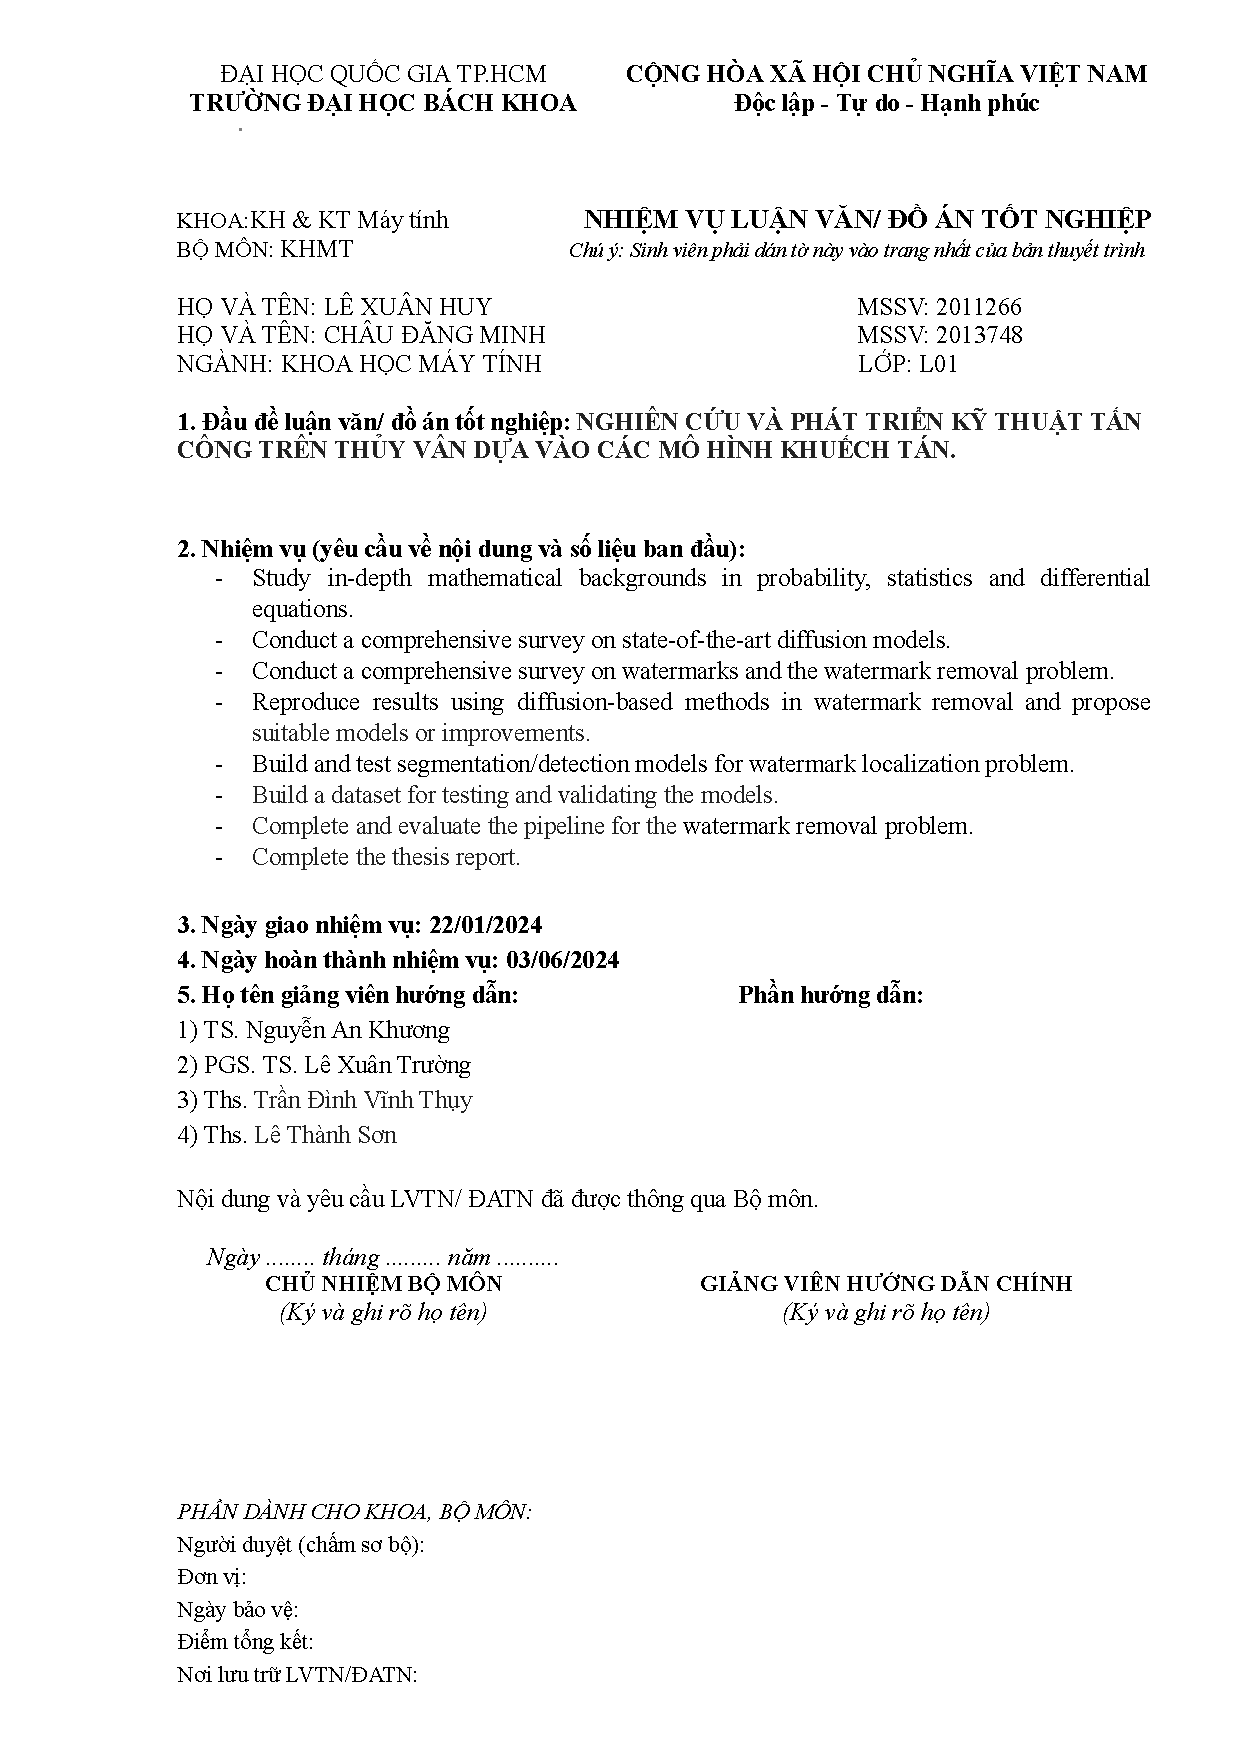
\includepdf{img/PhieunhiemvuLVTN-DATN.docx.pdf}

\chapter*{Declaration}
We certify that this capstone project ``Research and Develop Diffusion-based Attacks on Watermark'' is our research under the supervision of Dr. Nguyen An Khuong, Assoc. Prof. Le Xuan Truong, Mr. Le Thanh Son and Mr. Tran Dinh Vinh Thuy and derived from practical needs and our desire to study. We also declare that everything written in this report, except for which from the references in Bibliography section, is the result of our research and has never been published before.

\null\hfill Authors
\chapter*{Acknowledgements}

This capstone project, an essential milestone for our graduation, would not have been possible without the support of many individuals. We extend our heartfelt gratitude to our dedicated supervisors Dr. Nguyen An Khuong for, Assoc. Prof. Le Xuan Truong, Mr. Le Thanh Son, and Mr. Tran Dinh Vinh Thuy, our dedicated supervisors, for their unwavering guidance and support throughout this journey. Their expertise and feedback every hour in the meetings have been invaluable.

We also wish to express our sincere thanks to the lecturers at Ho Chi Minh City University of Technology, particularly those from the Faculty of Computer Science and Engineering, for imparting their knowledge and wisdom over the past four years. Lastly, we are profoundly grateful to our families and friends for their unwavering support and encouragement throughout our academic endeavors.

\chapter*{Abstract}
In our capstone project, we utilize semantic segmentation models and a diffusion-based model named Image-to-Image Schrödinger Bridge (I$^2$SB) with an aim to remove visible watermarks out of original images. The work is attainable by the ability of diffusion models to transform a sample from one distribution to another. We proposed a comprehensive pipeline that processes a watermarked image and outputs an unwatermarked version while preserving the original structure of the image. Theoretical underpinnings of these models, namely stochastic differential equations and the widely-recognized Transformer architecture are also delved diligently into. 

\textbf{Keywords:} segmentation, diffusion-based models, watermark removal.
\chapter*{List of Frequently Used Notations and Symbols}
\addcontentsline{toc}{chapter}{List of Frequently Used Notations and Symbols}

\renewcommand{\arraystretch}{1.2}
\begin{tabular}{ll}
 $\NN$              & The set of positive integers                                                        \\
 $\NN_0$            & The set of non-negative integers                                                    \\
 $\QQ$              & The set of rational numbers                                                         \\
 $\RR$              & the set of real numbers                                                             \\
 $\RR_+$            & the set of non-negative real numbers                                                \\
  $\P $              & a property                                                                          \\
  $\{X_i\}_{i\in I}$ & A family of objects $X_i$ where $i$ is in the index set $I$                         \\
 $(X_i)_{i\in I}$   & A sequence of objects $X_i$ where $i$ is in the index set $I$                       \\
   $\F,\G$       & $\sigma$-algebras                    \\
  $\sigma(\C)$       & the $\sigma$-algebra generated by a collection $\C$ of subsets                      \\
 $\sigma(X)$        & the $\sigma$-algebra generated by a random variable $X$                             \\
  $\mu$              & a measure                                                                           \\
 $\lambda$          & the Lebesgue measure                                                                \\
 $\PP$              & a probability measure                                                               \\
 $\Y^\X$            & \text{the set of functions from $\X$ to $\Y$}                                    \\
  $C^2_0(U)$         & the set of twice differentiable functions with compact support on $U$               \\
  $L^2(\mu)$         & the $L^2$ space of measurable functions with respect to the measure $\mu$           \\
 $\L^2(\PP)$        & the $\L^2$ space stochastic processes with respect to the probability measure $\PP$ \\
 $\EE[\cdot]$       & the expectation                                                                     \\
 $|x|$              & The absolute value of a real number $x$                                             \\
 $\|\mathbf{x}\|_p$ & the $p$-norm of a vector $x\in\RR^d$                                                \\
 $\|X\|_{L^p}$ & the $L^p$-norm of a $L^p$ random variable $X$                                              \\
 $\|X\|_{\L^p}$ & the $\L^p$-norm of a $L^p$ stochastic process $X$                                              \\
 $\mathbf{1}_A$     & the indicator function over a set $A$                                               \\
 $\delta_A$         & the Dirac delta distribution with respect to a set $A$                              \\

\end{tabular}
\renewcommand{\arraystretch}{1}
\pagestyle{empty}
\tableofcontents
\newpage
% \addcontentsline{toc}{chapter}{List of Figures}

\listoffigures
\listoftables
\pagestyle{fancy}
\chapter{Introduction}
\label{chapter:intro}
A watermark is an additional message embedded in the original work. Initially, watermark embedding techniques were developed to mark the manufacturing process. Over time, watermarks have been widely adopted to protect the integrity and authenticity of content, ensuring that products are not stolen by others. Digital watermarking techniques have been proposed and developed for various types of media, including images, audio, video, and text \cite{cox2007digital}. These techniques often employ advanced methods such as deep neural networks \cite{luo2023dvmark}, wavelet transforms, singular value decomposition \cite{ernawan2020block}, and edge detection \cite{kadian2021robust} to ensure high imperceptibility, robustness, capacity, and security. Additionally, some techniques consider human perception and application scenarios to optimize performance. However, authorized users often wish to remove watermarks from their images as these marks can be distracting or obscure essential details. Using image-editing software such as Photoshop for this task typically requires significant time and expertise. An automated solution for watermark removal, especially in videos, would be a valuable asset. Conversely, the problem of watermark removal has become a promising research topic as it counteracts watermark embedding. As solutions for removal become more efficient, both embedding and removal problems have evolved into subbranches of security and steganography, each advancing the other. 

Recently, several methods have been proposed to tackle this problem using various approaches, many of which utilize deep neural networks (DNNs). AdvancedUnet \cite{wei2023visual} employs the strong image translation performance of the U-structure network (U-net) to simultaneously extract and remove watermarks. Generative Adversarial Networks (GANs) such as cGAN \cite{liu2021wdnet, sun2021detect} are also used to detect and reverse watermarks within the DNNs. Other approaches leverage attention mechanisms to identify and remove watermark regions, such as the Attention-based DNN \cite{zhang2021blind}. Diffusion models have demonstrated remarkable results in generating high-quality images, surpassing GANs in some cases \cite{dhariwal2021diffusion} and thus have found their applications in watermark removal \cite{li2023diffwa}.


% Another approach involves image-to-image translation to learn the mapping between watermarked and clean images, such as with cGAN \cite{liu2021wdnet}. Some methods leverage attention mechanisms to identify and remove watermark regions, such as the Attention-based DNN \cite{zhang2021blind}.

% The advancements of computational performance and ongoing theoretical research have led to significant progress in the functionality of Machine Learning on large datasets. Beyond making decisions and deriving insights, recent models can generate new samples that resemble their training datasets. These models are known as Generative Models. For images and sounds, the generated samples are not only perceptible but often highly aesthetic. \textcolor{red}{Notable examples include Generative Adversarial Networks (GANs) \cite{goodfellow2014generative}, Variational Auto-Encoders (VAEs) \cite{hinton2006reducing}, and Diffusion Models \cite{sohl2015deep}}. 


% Additionally, the breakthrough Transformer architecture \cite{vaswani2017attention} has inspired the application of Natural Language Processing solutions to Computer Vision, resulting in state-of-the-art performance that outstrips traditional Convolutional Neural Network (CNN) methods.


These developments paved the way for our capstone project. We utilize a diffusion-based inpainting model, the Image-to-Image Schrödinger Bridge (I$^2$SB) \cite{liu2023i2sb}, along with a zero-shot segmentation model, Segment Anything Model (SAM) \cite{kirillov2023segment}, to address the intriguing problem of removing watermarks from media data.


\section{Introduction to the Problem}
In this project, we apply the Image-to-Image Schrödinger Bridge (I$^2$SB) and Segment Anything Model (SAM) to remove watermarks from images. In machine learning terms, this involves transforming a sample from the distribution of watermarked images to a sample from the distribution of clean images, while preserving the overall content and information of the images. The proposed approach can serve as a benchmark for further research in the field of watermark generation and removal. The state-of-the-art performance of these models, combined with our desire to understand their mechanisms, motivates us to undertake this project. Therefore, we also delved into the relevant mathematical and neural network concepts to gain a thorough understanding of the mechanisms underlying these models. Despite the theoretical and technical challenges, our work is structured around the following objectives:

\begin{enumerate}
    \item Study in-depth the principles of mathematical analysis, including measure theory and probability theory, which contribute to the theory of stochastic processes and stochastic differential equations. Our goal is to achieve a clear understanding of the main theoretical result, the principal theorem of reverse-time diffusion models.
    \item Study the theory of Artificial Neural Networks, with a focus on understanding the Transformer architecture.
    \item Using the acquired knowledge, examine predominant diffusion models such as Denoising Score Matching (DSM), Denoising Diffusion Probabilistic Models (DDPM) and Score-based Generative Models (SGM) through stochastic differential equations. We will also study the closely related result for our problem, the Image-to-Image Schrödinger Bridge (I$^2$SB). Additionally, we delve into the architecture of transformer-based models for image segmentation, including Vision Transformer, SegFormer, and the Segment Anything Model.
    \item Test SAM and Image-to-Image Schrödinger Bridge on a lightweight image dataset embedded with a watermark dataset. 
\end{enumerate}

\section{Scope of the Project}
We have selected a lightweight version of the ImageNet dataset for our project due to its widespread use and its comprehensive coverage of common objects and scenarios. To incorporate watermarks, we have chosen images from the Pokémon dataset, reflecting our interest in cartoons.

\section{Report Structure}
The main structure of our project is as follows:

\textbf{Chapter I. Introduction.} This chapter provides an overview of generative models and segmentation models, as well as watermark embedding and removal techniques. It outlines our research problem and the objectives we aim to achieve in the project.

\textbf{Chapter II. Mathematical Preliminaries.} We discuss the essential building blocks for diffusion models, including measure theory, probability theory, stochastic processes, and stochastic differential equations.

\textbf{Chapter III. Machine Learning Foundation.} This chapter delves into several key diffusion models, encompassing the unconditional diffusion model and the Denoising Diffusion Probabilistic Models (DDPM) \cite{ho2020denoising}. Along the way, we highlight the use of Stochastic Differential Equations (SDEs) to simply train the score function. We also explore the Schrödinger Bridge problem \cite{schrodinger1932theorie} as an example of conditional models.  Additionally, we examine the widely adopted Transformer architecture \cite{vaswani2017attention}, with an application to Computer Vision \cite{liu2018image}.

\textbf{Chapter IV. Related Works.} Here, we review previous research on watermark embedding and removal models, as well as other models related to our removal pipeline, including SegFormer, SAM, and I$^2$SB.

\textbf{Chapter V. Proposed Method and Experiments.} In this chapter, we propose our detailed two-stage pipeline for solving the watermark removal problem, applying related works SAM and I$^2$SB. We then present the results of SAM and I$^2$SB in watermark removal against several other models on a lightweight version of the ImageNet dataset, with watermarks sourced from the Pokémon dataset.

\textbf{Chapter VI. Conclusion.} This chapter summarizes the work done in the project, identifies limitations, and discusses plans for future improvements.

\textbf{Appendix.} This section contains relevant extended inferences and supplementary information.









\chapter{Mathematical Preliminaries}
\thispagestyle{empty}
In this chapter, we build step-by-step preliminaries in mathematical analysis that establish diffusion models. Discrete-time diffusion models are based on Markov chains, which is a stochastic process, and continuous-time are based on stochastic differential equations, both are derived from probability theory. Therefore, we begin by discussing the basics of mathematical analysis needed to develop formal probability theory. From probability theory, we study stochastic processes, stochastic integrals and stochastic differential equations.


\section{Mathematical Spaces}
\subsection{Motivations}

When working with the set of real numbers $\RR$, we are familiar with the absolute value defined $x\in\RR$
\begin{equation}
 \label{equation:number-absolute-value}
 |x| = \begin{cases}
  x, \text{ if } x\ge0 \\
  -x, \text{ if } x < 0.
 \end{cases}
\end{equation}
The distance between two real numbers $x$ and $y$ is $|x-y|$. We also concern about sequences of real numbers with properties such as boundedness and convergence. A sequence $(x_n)_{n\in\NN}\subset\RR$ is bounded if
$$\exists M\in\RR, \forall n\in \NN, |x_n|\le M.$$
The sequence $(x_n)_{n\in\NN}\subset\RR$ converges to a limit $x$ if
$$\forall \epsilon > 0, \exists N\in\NN, \forall n>N, |x_n-x|<\epsilon.$$

These concepts have been generalized to $\RR^d$. For each vector $\xbf=(x_1,\ldots,x_d)\in\RR^d$, the absolute value becomes the norm
\begin{equation}
 \label{equation:vector-norm}
 \|\xbf\| = \sqrt{x_1^2+\ldots+x_2^d}.
\end{equation}
The distance between two vectors $\xbf$ and $y$ is $|\xbf-\ybf|$. The norm is a real number, and it lets us define properties of sequence as in $\RR$. This is actually the evolution of mathematics: mathematicians first work with real-life objects, such as arithmetic numbers or Euclidean geometry shapes, then discover the same pattern with another objects, such as the vectors. Then, they developed an abstract structure covering these objects, ignoring the very details, such as the vector space. The abstraction progress really fulfills the picture of mathematics, and extends mathematics applications. In forthcoming sections, we will see the benefits of following introductory concepts. For example, we can regard a specific class of random variables (see Definition \ref{definition:random-variable}) and stochastic processes (see Definition \ref{definition:stochastic-process}) akin to the real numbers. Such abstractions graciously facilitate to further developments relating to the studied objects.

Motivated enough, we are going to generalize these concepts of norm, distance and convergence in following discussions by three spaces, namely metric space, normed space and Banach space.

\subsection{Metric Space}

\begin{definition}
 Given a set $\Omega$. A function $d:\Omega\times\Omega\to\RR$ is called a \textbf{metric} if it satisfies
 \begin{enumerate}
  \item Non-negativity: $d(x,y)\ge 0,\forall x,y\in\Omega$. The equality holds if and only if $x=y$.
  \item Symmetry: $d(x,y)=d(y,x)$.
  \item Triangle inequality: $d(x,y)+d(y,z)\ge d(x,z)$.
 \end{enumerate}
 The tuple $(\Omega,d)$ is called a \textbf{metric space}\index{metric space}.
\end{definition}

\begin{example}
 \begin{enumerate}
  \item []
  \item Given a set $\Omega$ and a function $d:\Omega\times\Omega\to\RR$ defined by
        $$d(x,y)=\begin{cases}
          1, & \text{ if } x=y     \\
          0, & \text{ if } x\ne y.
         \end{cases}$$
        Then $d$ is a metric
  \item Let $(\Omega, \|\cdot\|)$ be a normed space. Define $$d(x,y) = \|x-y\|, \forall x,y\in\Omega.$$
        Then $d$ is a metric.
 \end{enumerate}
\end{example}

\begin{definition}
 Let $(\Omega, d)$ be a metric space. A subset $A$ of $\Omega$ is said to be \textbf{open}\index{open} if for any $x\in A$, there exists $\epsilon > 0$ such that if a point $y$ having $d(x, y)<\epsilon$, then $y\in A$.
\end{definition}

\begin{definition}
 Let $(\Omega, d)$ be a metric space. A sequence $(x_n)_{n=1}^\infty\subset\Omega$ is said to \textbf{converge}\index{convergence} to $x\in\Omega$ if
 $$\forall \epsilon>0, \exists N>0,\forall n> N, x_n\in B_\epsilon(x).$$
\end{definition}

\begin{definition}
 A metric space $\Omega$ is said to be \textbf{complete} if every convergent sequence in $\Omega$ has the limit in $\Omega$.
\end{definition}

\subsection{Normed Space}

\begin{definition}
 Let $K$ be a filed and $V$ be a vector space over $\mathbb{K}$. A function $\|\cdot\|: V\to \RR$ is called a \textbf{norm}\index{norm} if it satisfies
 \begin{enumerate}
  \item Non-negativity: $\|x\|\ge0,\forall x\in V$. The equality holds if and only if $x=0$.
  \item Absolute homogeneity: $\|\lambda x\| = |k|\cdot\|x\|,\forall x\in V, \lambda\in\mathbb{K}$.
  \item Triangle inequality: $\|x\|+\|y\|\ge \|x+y\|,\forall x,y\in V$.
 \end{enumerate}
 The tuple $(V,\|\cdot\|)$ is called a \textbf{normed space}\index{normed space}.
\end{definition}

\begin{example}
 \begin{enumerate}
  \item []
  \item Regard $\RR^d$ as a real vector space. For each $p\in[1,\infty]$, defined the function $\|\cdot\|_p:\RR^d\to\RR$ for each $\|\xbf\|_p = (x_1,\ldots, x_n)$ by
        \begin{equation}
         \|\xbf\|_p = \begin{cases}
          \left(\sum\limits_{i=1}^d |x_i|^p\right)^{1/p}, & \text{ if } p <\infty \\
          \sup\{x_i, \,\,1\le i \le d\}.,                 & \text{ if } p =\infty
         \end{cases}
        \end{equation}
        Then $\|\cdot\|_p$ is a norm, called the $p$-norm of $\RR^d$.
  \item Regard $\RR^{d\times r}$ as a real vector space. Let function $\|\cdot\|_F: \RR^{d\times r}\to\RR$ be defined for each $\Abf = (a_{ij})\in\RR^{m\times n} $ as
        $$\|A\|_F = \sqrt{\sum\limits_{i=1}^m\sum\limits_{j=1}^na_{ij}^2}.$$
        Then $\|\cdot\|_F$ is a norm, called the Frobenius norm.
 \end{enumerate}
\end{example}

% \begin{theorem}[Cauchy-Schwartz inequality]
%   \label{cauchy-schwartz-inequality}
% \end{theorem}

\subsection{Banach Space}
\begin{definition}
 A \textbf{Banach space}\index{Banach space} is a normed space that is complete with respect to the metric induced by the norm.
\end{definition}

\section{Measure Theory and Integration}
\subsection{Measure Space}
In the normal sense of the word ``measure'', the measure of any interval $I=[a,b]$, in $\RR$ coincides with the length $\ell(I)=|b-a|$. Similarly, the area of a square $S = [a_1,b_1]\times [a_2,b_2] = I_1\times I_2$ in $\RR^2$ is $\ell(I_1)\cdot\ell(I_2)$. More generally, given intervals $I_k = [a_k,b_k], k = 1,\ldots, n$, the volume of the box $B= I_1\times \ldots \times I_n$ in  $\RR^n$ is $\prod\limits_{k=1}^n \ell(I_k)$. Measure theory generalizes the length, area and volume to other measures on other abstract sets $\Omega$ rather than $\RR^n$. Moreover, this branch of real analysis establishes the class of measurable subsets of $\Omega$. To see the reason for this diligent work of mathematicians on measure theory, let us take an example on the measure of length. As in ordinary contexts, the length $\ell(E)$ of any subset $E$ of $\RR$, if exists, is required to satisfy

\begin{enumerate}
 \item Non-negativity: $\ell(E) \ge 0$.
 \item If $E\subset F\subset \RR$, then $\ell(E)\le \ell(F)$.
 \item If $E=[a,b]$, then $\ell(E) = |b-a|$.
 \item Translation invariance: for any $x\in\RR$, $\ell(E+x) = \ell(E)$.
 \item If $E$ can be divided to a collection of disjoint intervals $\{I_k\}_{k\in N}$, assuming that $\ell(\varnothing) = 0$, then $\ell(E) = \sum\limits_{k=1}^\infty \ell(I_k).$
\end{enumerate}

We will prove that our intuitive length measure cannot be applied for all subsets of $\RR$ \cite{vitali1905sul}.

\begin{proposition}
 If there exists $\ell : 2^\RR \to [0,\infty]$ satisfying
 \begin{enumerate}[label=(\arabic*)]
  \item If $E=[a,b]$, then $\ell(E) = |b-a|$. Also assume that $\ell(\varnothing) = 0$.
  \item If $E\subset F\subset \RR$, then $\ell(E)\le \ell(F)$.
  \item Translation invariance: for any $x\in\RR$, $\ell(E+x) = \ell(E)$.
  \item If $E$ can be divided to a collection of disjoint intervals $\{I_k\}_{k\in N}$, then $\ell(E) = \sum\limits_{k=1}^\infty \ell(I_k).$
        % \item (Derived from (2) and (4)) for any collection  measurable sets $\{A_k\}_{k=1}^{\infty}$,
        %       $$\ell\left(\bigcup\limits_{k=1}^{\infty} A_k\right) \le \sum_{k=1}^{\infty} A_k.$$
 \end{enumerate}
 Then $\ell(E) = 0, \forall E\in 2^\RR$.
\end{proposition}

\begin{proof}
 By (2), we have $\ell((0,1])\le \ell([0,1]) = 1$. Let us define an equivalence relation \index{equivalence relation} on $(0,1]$ as
 $$x\sim y \Leftrightarrow x-y\in\QQ.$$
 Clearly, for any $x\in (0,1]$, we have the equivalence class
 $$[x] = \{y\in(0,1] : x-y\in \QQ\} = \{x+q: q\in \QQ, x+q\in (0,1]\}.$$
 Denote by $N\in\NN\cup\{\infty\}$ the number of equivalence classes. Choose an element $x_n$ from the $n$-th equivalence class, where $1\le n\le N$\footnote{We have made use of the Axiom of Choice}. Clearly all the $x_n, n\in1,\ldots, N$ are distinct.

 Let $A=\{x_k\}_{k=1}^N\subset(0,1]$ and $(q_n)_{n=1}^\infty$ be a numeration of $\QQ\cap(-1,1]$\footnote{The set of rational number $\QQ$ is countable}. Also, let $A_n = A + q_n$ for any $n\in\NN$. We claim that if $n\neq m$, then $A_n\cap A_m = \varnothing$. We will prove the contrapositive statement. Suppose that there exists $x\in A_n\cap A_m$, then $x=a_n + q_n = a_m + q_m$, where $a_n\in A_n$ and $a_m\in A_m$. Therefore,
 $$a_n-a_m = q_m-q_n\in \QQ,$$
 which implies that $a_n\sim a_m$. Hence, $a_n$ and $a_m$ are presentations of a single equivalent class, or $n=m$.

 On the other hand, $(0,1] \subset \bigcup\limits_{n=1}^\infty A_n \subset (-1,2]$.

 By (3) and (4),
 $$\ell((-1,2]) = \ell((-1,0]) + \ell((0,1]), \ell((1,2]) = 3\ell((0,1]).$$

 By (3), we have

 $$\ell(A_n) = \ell (A), \forall n\in\NN.$$

 By (4) and the previous implications,
 $$\ell((0,1]) \le \ell\left(\bigcup\limits_{n=1}^\infty A_n\right) = \sum\limits_{k=1}^{\infty} \ell(A_k) = \sum_{k=1}^{\infty} \ell(A) \le 3\ell((0,1]).$$

 This implies $\ell(A)=0$, and also $\ell((0,1])=0$. Therefore,

 $$\ell(\RR) = \ell\left(\bigcup\limits_{m\in\ZZ}(m,m+1] \right) = \sum\limits_{m\in\ZZ} \ell((m,m+1])= \sum\limits_{m\in\ZZ} \ell((0,1]) = 0.$$

 Thus, $\ell$ coincides with the zero function. However, this measure of length is unavailing.
\end{proof}


A measure space is the initial model to measure theory. Consider the following real-life example.

\begin{example}
 A farmer has a rectangular land whose width and length are both $100\,m$. The coordinated representation of the land is $\Omega=[0,100]\times[0,100]$. The farmer allocates a region to build a warehouse, whose shape is not restricted to be a rectangle. To approximate the area of this region, the farmer divides it into disjoint rectangular subregions and sums of the areas.
\end{example}

A region is a set of $\Omega$. We know that maybe some subsets of $\Omega$ cannot be measured. Let $\F\subset2^\Omega$ be the family of all measurable subsets of $\Omega$. The area of whole land is known by the farmer i.e. $\Omega\in\F$. On the other hand, if we can measure the area of the warehouse, the rest region's area can also be measured. Motivated by the context, the set of measurable regions as above is defined formally as a $\sigma$-algebra, as below.

\begin{definition}
 \label{definition:sigma-algebra}
 Given a set $\Omega$. A collection of subsets $\F$ of $\Omega$ is called a \textbf{$\sigma$-algebra}\index{$\sigma$-algebra} if
 \begin{enumerate}
  \item $\varnothing, \Omega\in\F$;
  \item If $A\in\F$, then $A^c\in\F$;
  \item If $A_1,A_2,\ldots\in\F$, then $A_1\cup A_2\cup\ldots\in\F$.
 \end{enumerate}
 The pair $(\Omega, \F)$ is called a \textbf{measurable space}\index{measurable space}.
\end{definition}

Definition \ref{definition:sigma-algebra} models measurable objects to be a collection $\F$ of subsets of a given set $\Omega$. Before the definition of a measure, we consider some examples and analytically derived theorems.

\begin{example}
 \label{example:1}
 Given a set $\Omega$, then $\{\varnothing, \Omega\}$ and the power set $2^\Omega$ are two trivial $\sigma$-algebras. Let $\Omega=\{1,2,3\}$, the collection $\F=\{\varnothing,\Omega, \{1\}, \{2,3\}\}$ is a $\sigma$-algebra on $\Omega$.
\end{example}

\begin{proposition}
 Let $\{\F_\alpha\}_{\alpha\in I}$ be an arbitrary family of $\sigma$-algebras on $\Omega$. Then the intersection $\F=\bigcap\limits_{\alpha\in I}\F_\alpha$ is a $\sigma$-algebra.
\end{proposition}

\begin{proof}
 We will check that $\F$ three conditions for a $\sigma$-algebra.

 Since $\varnothing,\Omega\in\F_\alpha,\forall\alpha\in I$, we have $\varnothing,\Omega\in\bigcap\limits_{\alpha\in I}\F_\alpha$.

 If $A\in\bigcap\limits_{\alpha\in I}\F_\alpha$, then $A\in \F_\alpha,\forall\alpha\in I$, leading to $A^c\in \F_\alpha,\forall\alpha\in I$. Hence, $A^c\in\bigcap\limits_{\alpha\in I}\F_\alpha.$

 Finally, if $A_i\in\F_\alpha,\forall i\in\ZZ^+,\forall \alpha\in I$, then $\bigcup\limits_{i\in\ZZ^+}A_i\in\F_\alpha,\forall\alpha\in I$. Therefore,
 $\bigcup\limits_{i\in\ZZ^+}A_i\in\bigcap\limits_{\alpha\in I}\F_\alpha.$
\end{proof}

\begin{remark}
 The union of $\sigma$-algebras on $\Omega$ is not necessarily a $\sigma$-algebra. For example,
 $$\F_1=\{\varnothing,\Omega, \{1\}, \{2,3\}\} \text{ and } \F_2=\{\varnothing,\Omega, \{2\}, \{1,3\}\}$$
 are two $\sigma$-algebras on $\Omega=\{1,2,3\}$, but
 $$\F=\F_1\cup\F_2=\{\varnothing,\Omega,\{1\},\{2\},\{2,3\},\{1,3\}\}$$ is not, since $\{3\}=\{2,3\}\cap\{1,3\}\notin \F$.
\end{remark}

Having mentioned in Example \ref{example:1}, any collection $\C$ of subsets of $\Omega$, has a trivial $\sigma$-algebra $2^\Omega$ that contains $\C$ i.e. $\C\subset2^\Omega$. Therefore, there exists the smallest $\sigma$-algebra containing $\C$.

\begin{theorem}
 \label{theorem:generated-sigma-algebra}
 Given a set $\Omega$ and a collection of its subsets $\C$, there exists the smallest $\sigma$-algebra containing $\C$, denoted by $\sigma(\C)$, given by
 $$\sigma(\C)=\bigcap\limits_{\alpha\in I}\F_\alpha,$$
 where $\{\F_\alpha\}_{\alpha\in I}$ is the set of $\sigma$-algebras containing $\C$. We also called $\sigma(\C)$ to be the $\sigma$-algebra generated by $\C$.
\end{theorem}

\begin{proof}
 Since $\sigma(\C)$ itself is a $\sigma$-algebra containing $\C$ so $\sigma(\C)\in\{\F_\alpha\}$, leading to

 $$\bigcap\limits_{\alpha\in I}\F_\alpha\subset \sigma(\C).$$

 Moreover, $\bigcap\F_i$ is also a $\sigma$-algebra containing $\C$ and $\sigma(\C)$ is the smallest one, hence

 $$\sigma(\C)\subset\bigcap\limits_{\alpha\in I}\F_i.$$

 Thus, $\sigma(\C)=\bigcap\limits_{\alpha\in I}\F_i$.
\end{proof}

\begin{remark}
 Theorem \ref{theorem:generated-sigma-algebra} tells us that a collection of measurable subsets can be extended to a $\sigma$-algebra. For example, a collection $\C=\{\{1\}\}$ of subsets of $\Omega=\{1,2,3\}$ generates the $\sigma$-algebra
 $$\F=\{\varnothing,\Omega,\{1\},\{2,3\}\}.$$
\end{remark}

\begin{figure}[ht]
 \centering
 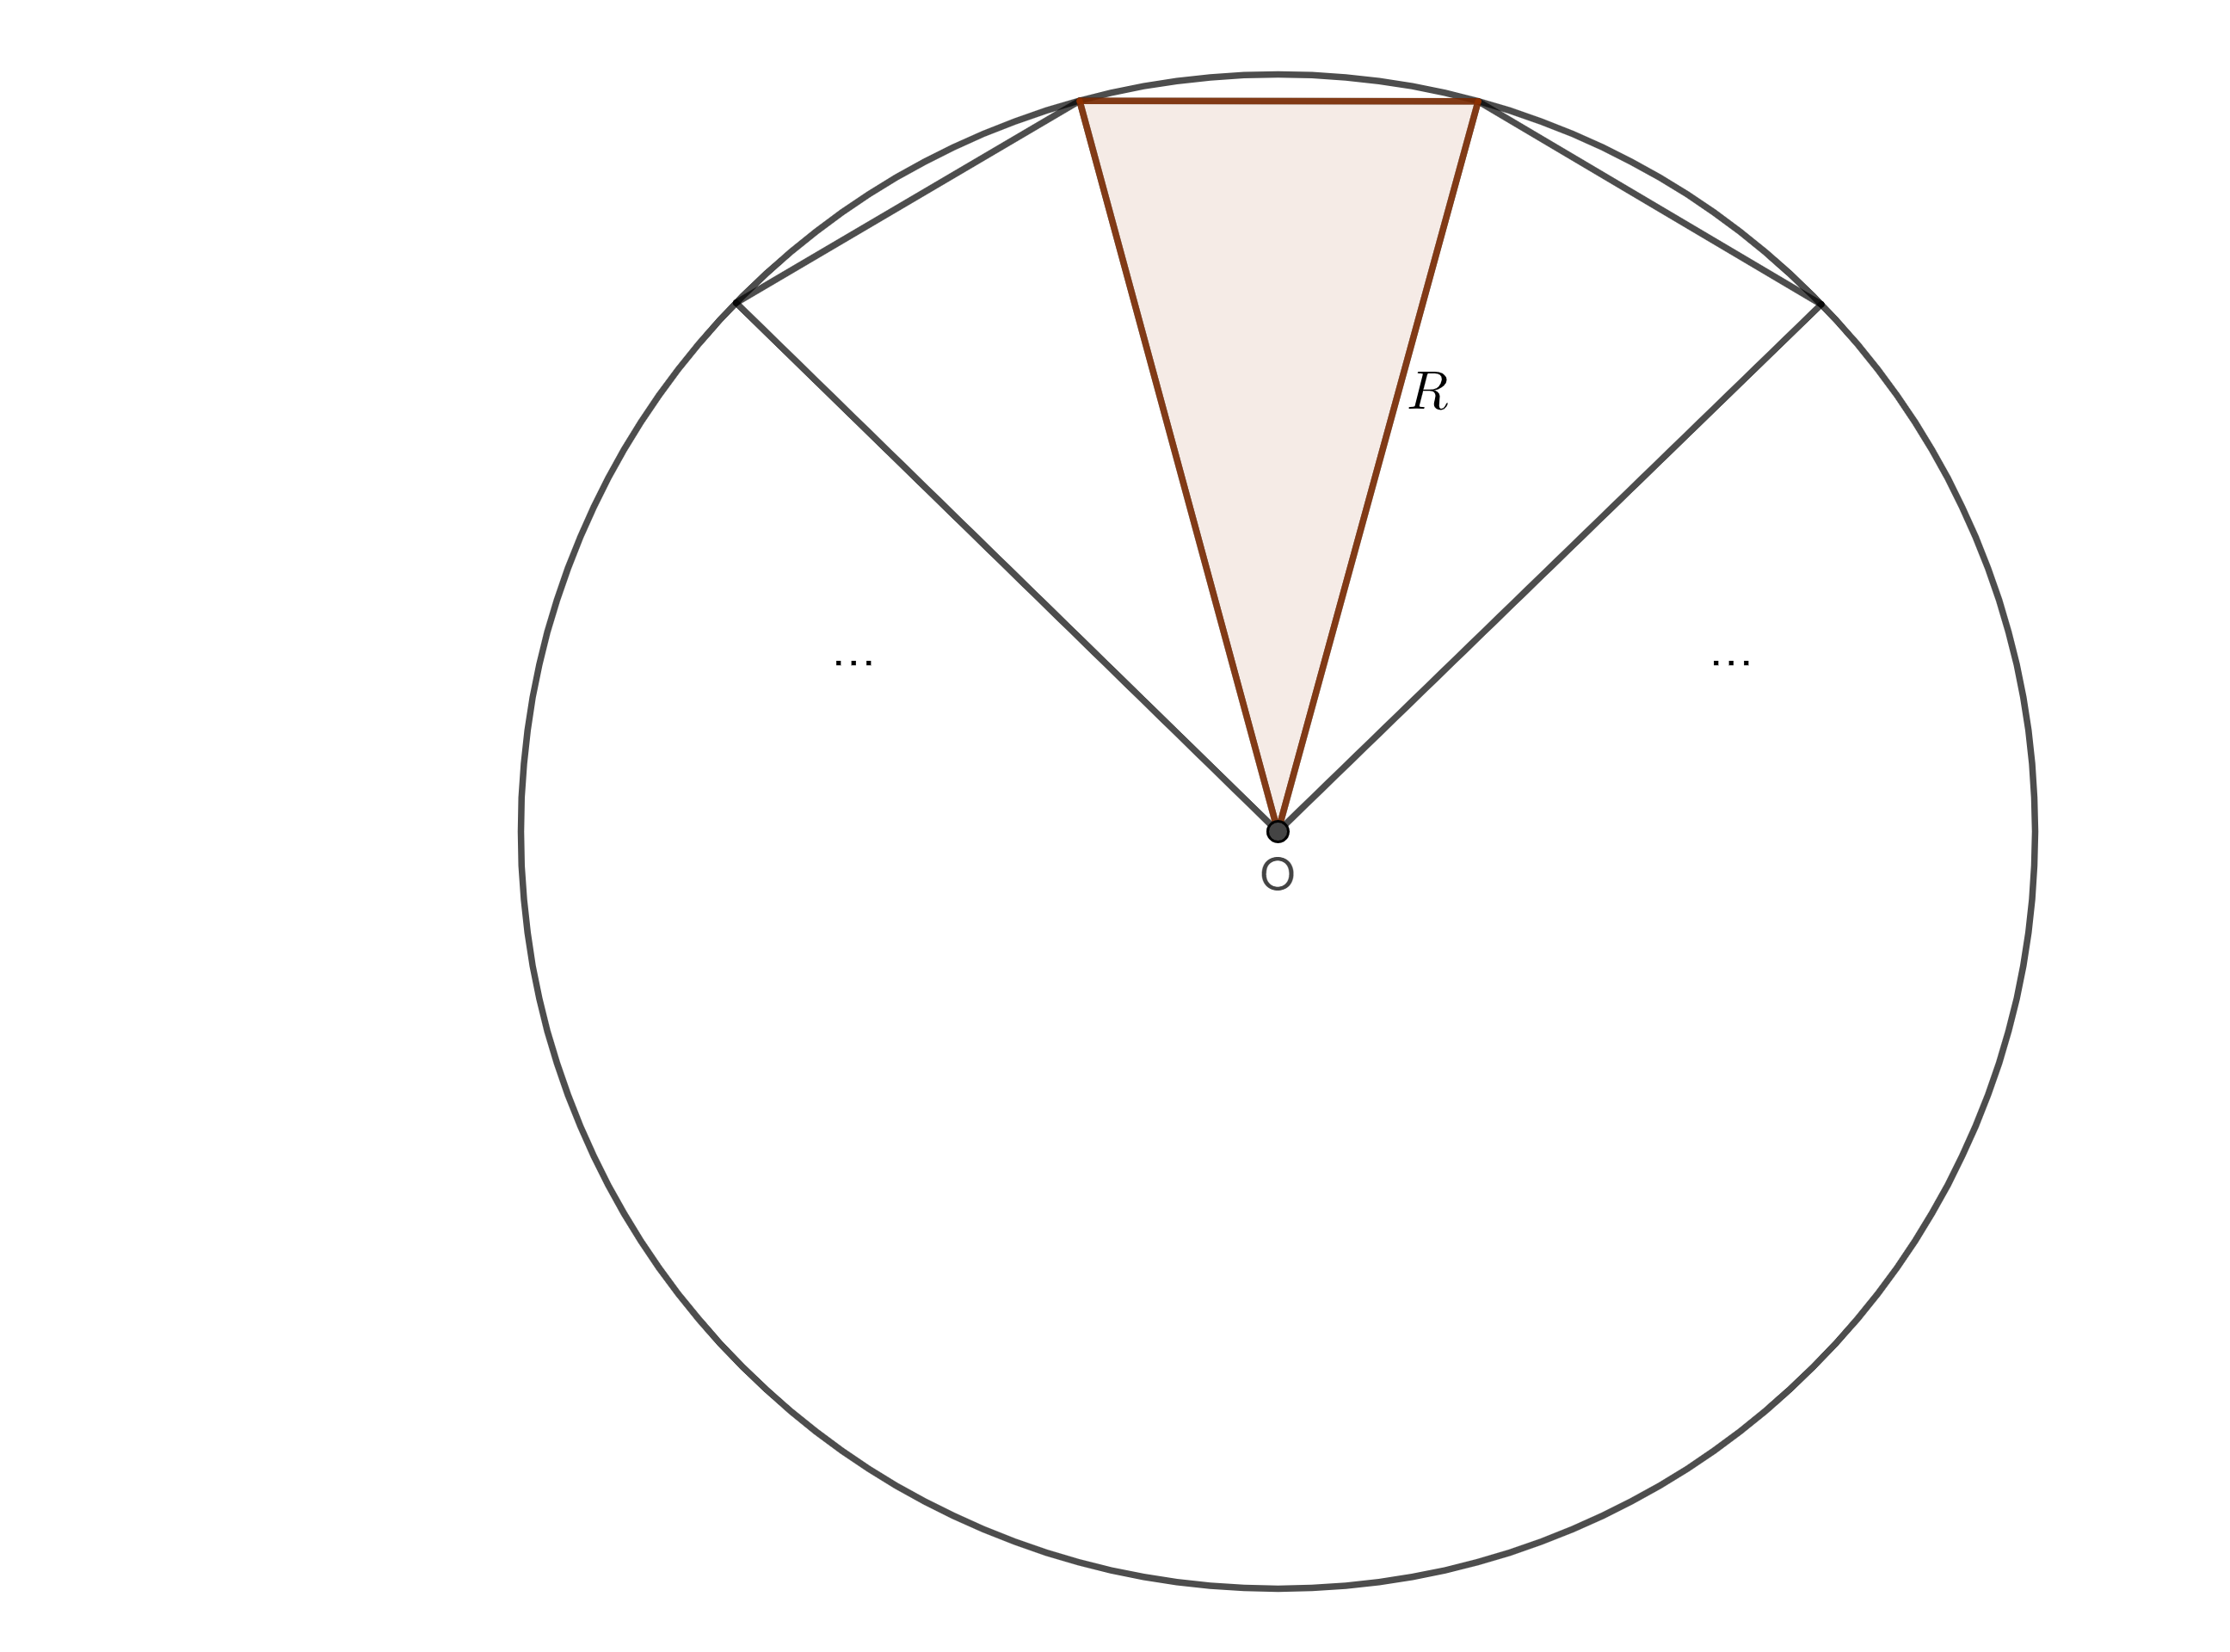
\includegraphics[width=0.4\linewidth]{img/circle.png}
 \vspace{0.5cm}
 \caption[Circle area approximation]{The area of a circle can be calculated by dividing it into equal isosceles triangles. As the number of triangles tends to infinity, the sum of bottom sides tends to the perimeter $2\pi R$ of the circle and the attitude of a triangle tends to $R$. Hence, the area is $A=\dfrac{1}{2}(2\pi R)R=\pi R^2$.}
 \label{figure:circle}
\end{figure}

\begin{definition}
 Given a measurable space $(\Omega,\F)$, a function $\mu:\F\to\RR$ is called a \textbf{measure}\index{measure} if it satisfies
 \begin{enumerate}
  \item Non-negativity: $\mu(A)\ge0,\forall A\in\F.$
  \item $\mu(\varnothing)=0$.
  \item Countable additivity: if $\{A_i\}_{i=1}^\infty\subset\F$ contains pairwise disjoint elements, then
        $$\mu\left(\bigcup\limits_{i=1}^\infty A_i\right)=\sum\limits_{i=1}^\infty \mu(A_i).$$
        The triplet $(\Omega,\F,\mu)$ is called a measure space.
 \end{enumerate}
\end{definition}

% \begin{theorem}[Properties of a measure]
%   \begin{enumerate}
%     \item[]
%     \item Monotonicity\index{monotonicity}: if $A\subset B$, then $\mu(A)\le\mu(B)$.
%   \end{enumerate}
% \end{theorem}

\begin{example}
 \begin{enumerate}
  \item []
  \item Consider the measurable space $(\RR, \B(\RR))  $. The function of taking the length of open intervals on the real line
        $$\mu((x,y))=|y-x|,\forall x,y\in\RR,$$
        which an assumption that $\mu(\varnothing)=0$, is a measure. Three properties of a measure are satisfied trivially.
  \item Consider the measurable space $(\RR, \F)$, where $\F$ is any $\sigma$-algebra on $\RR$. Given $a\in\RR$. The indicator function $\mathbf{1}_a: \F\to\{0,1\}$ given by
        $$\begin{cases}
          \mathbf{1}_a(X)=1, & \text{ if } a\in X \\
          \mathbf{1}_a(X)=0, & \text{ otherwise }
         \end{cases}$$
        is a measure. We already have $\mathbf{1}_a(X)\ge0, \forall a\in X$. Let us check the other two properties of a measure for this function.
        \begin{itemize}
         \item Since $a\notin\varnothing$, we have $\mathbf{1}_a(\varnothing)=0$.
         \item For disjoints $X_1,X_2,\ldots$ it cannot be the case that there are two of them contain $a$. If $a\notin X_k,\forall k\in\ZZ^+$, then countable additivity holds since both sides are zero. Otherwise, if there exists $k\in \ZZ^+$ such that $a\in X_k$, then it follows that $$a\notin X_\ell, \forall \ell\ne k,$$ implying both sides are one.
        \end{itemize}
 \end{enumerate}
\end{example}

Given measure spaces $(\Omega,\F,\mu)$ and $(\Gamma,\G,\nu)$, we also concern about which pair $(x,\gamma)\in\Omega\times\Gamma$ that can be measured and how to measure them.

\begin{definition}
 Let $(\Omega,\F,\mu)$ and $(\Gamma,\G,\nu)$ be measure spaces. The \textbf{product $\sigma$-algebra}\index{product $\sigma$-algebra} $\F\otimes\G$ on $\Omega\times\Gamma$ is given by
 $$\F\otimes\G=\sigma(\{A\times B : A\in\F,B\in\G\}).$$
\end{definition}

\begin{definition}
 Let $(\Omega,\F,\mu)$ and $(\Gamma,\G,\nu)$ be measure spaces. The \textbf{product measure}\index{product measure} $\lambda(A\times B)$ on $\F\otimes\G$, where $A\in\F,B\in\G$ is given by
 $$\lambda(A\times B)=\mu(A)\nu(B)$$
\end{definition}

\begin{example}
 The measure of area $\mu$ in a two-dimensional space can be thought of as the product of two identical measures of length $\lambda$ in a one-dimensional space. Given two intervals $[a,b]$ and $[c,d]$, the equality
 $$\mu([a,b]\times [c,d])=\lambda([a,b])\cdot\lambda([c,d]),$$
 meets our intuition about the area of a rectangle. Here it also suggests that a rectangle with one size to be zero has area measure zero.
\end{example}

\begin{definition}
 \label{definition:property-almost-everywhere}
 Let $(\Omega, \F, \mu)$ be a measure space. A property $\P:\Omega\to\{\texttt{true},\texttt{false}\}$ is said to hold \textbf{almost everywhere}\index{almost everywhere} with respect to $\mu$, abbreviated by $\mu$-a.e. if
 $$\mu\left(\left\{x\in\Omega : \neg \P(x)\right\}\right) = 0.$$
\end{definition}

\subsection{Borel \texorpdfstring{$\sigma$}{σ}-algebra}

\begin{definition}
 Let $\mathcal{X}$ be a metric space. The $\sigma$-algebra $\B(\mathcal{X})$ \textbf{generated}\index{generated $\sigma$-algebra} by open subsets of $\mathcal{X}$ is called the Borel $\sigma$-algebra on $\mathcal{X}$. Each element in $\B(\mathcal{X})$ is called a Borel subset of $\mathcal{X}$.
\end{definition}

Borel $\sigma$-algebra is an essential class of $\sigma$-algebra. Borel $\sigma$-algebras on real vector spaces $\RR^d$ is later used to define random variables. These associated Borel $\sigma$-algebras can be thought of as containing all Lebesgue measurable and well-behave subsets of $\RR^d$.

\begin{proposition}
 \label{proposition:equivalent-borel-core}
 The Borel $\sigma$-algebra $\B(\RR)$ is generated by one of the following collections
 \begin{enumerate}[label=(\alph*)]
  \item the collection of all closed subsets of $\RR$;
  \item the collection of all intervals of the form $(-\infty,b]$;
  \item the collection of all intervals of R of the form $(a,b]$.
 \end{enumerate}
\end{proposition}

\begin{proof}
 Let $\B_1$, $\B_2$, and $\B_3$ be the $\sigma$-algebra generated by the collections of sets in parts (a), (b), and (c) of the proposition. We will show that
 $$\B(\RR)\supset \B_1 \supset \B_2 \supset \B_3 \supset \B(\RR).$$

 Since $\B(\RR)$ includes the family of open subsets of $\RR$ and is closed under complementation, it includes the family of closed subsets of $\RR$; thus it includes $\B_1$.

 The sets of the form $(-\infty,b]$ are closed and so belong to $\B_1$; consequently $\B_1 \supset \B_2$.

 Since $(a,b]=(-\infty,b]\cap(-\infty,a]^c$, each set of the form
 $(a,b]$ belongs to $\B_2$; thus $\B_2 \supset \B_3$.

 Finally, note that each open intervals of $\RR$ is the union of a sequence of sets of the form $(a,b]$ and that each open subset of $\RR$ is the union of a sequence of open intervals. Thus, each open subset of $\RR$ belongs to $\B_3$, and so $\B_3 \supset \B(\RR)$.
\end{proof}

\begin{proposition}
 The Borel $\sigma$-algebra $\B(\RR^d)$ is generated by one of the following collections
 \begin{enumerate}[label=(\alph*)]
  \item the collection of all closed subsets of $\RR^d$;
  \item the collection of all closed half-space of the form $\{(x_1,\ldots,x_d): x_1\le b_1,\ldots, x_d\le b_d\}$;
  \item the collection of all boxes of the form $\{(x_1,\ldots,x_d): a_1\le x_1\le b_1,\ldots,a_d\le x_d\le b_d\}$.
 \end{enumerate}
\end{proposition}

% \subsection{Lebesgue Measure}

% Lebesgue measure is the generalization of the length of subsets of $\RR$, and also the area and the volume for higher dimensional spaces. Let us denote Lebesgue measure on $\RR^n$ by $\lambda$, which we will construct later. Developed from the ordinary context of the length, area and volume, Lebesgue measure is required to satisfy translation invariance, i.e. for any $\lambda$-measurable set $A$ and $x\in\RR^n$, we have

% \begin{equation}
%   \label{equation:definition:translation-invariance}
%   \mu(A+x) = \mu(A).
% \end{equation}

% For any interval $I=(a,b)$ or $I=[a,b]$, define $\ell(I) = |b-a|$. For any subset $E\subset\RR$, the Lebesgue outer measure is defined as

% \begin{equation}
%   \label{equation:definition:lebesgue-outer-measure}
%   \lambda^*(E) = \inf\left\{\sum\limits_{k=1}^\infty\ell(I_k) : (I_k)_{k\in\NN} \text{ is a sequence of interval such that } E\subset\bigcup \sum\limits_{k=1}^\infty I_k\right\}.
% \end{equation}

\subsection{Measurable Map}

A measurable function is a function between the underlying sets of two measurable spaces that preserves the structure of the spaces: the preimage of any measurable set is measurable. This is in direct analogy to the definition that a continuous function between topological spaces preserves the topological structure: the preimage of any open set is open. Measurable functions are later used in the definition of the Lebesgue integral. In probability theory, a measurable function on a probability space is known as a random variable.

\begin{definition}
 Given two measurable spaces $(\Omega, \F)$ and $(\Gamma,\G)$. A map $f:\Omega\to\Gamma$ is said to be $(\F,\G)$-\textbf{measurable}\index{measurable map}  if
 $$f^{-1}(G)\in\F,\forall G\in \G.$$
\end{definition}

\begin{proposition}
 \label{preposition:preimage-of-a-measurable-map-over-the imaged-sigma-algebra-is-a-sigma-algebra}
 Given two measurable spaces $(\Omega, \F)$ and $(\Gamma,\G)$. If a map $f:\Omega\to\Gamma$ is $(\F\to\G)$-measurable, then the collection $\{f^{-1}(G) : G\in\G\}$ is a sub-$\sigma$-algebra of $\F$. Moreover, it is the smallest $\sigma$-algebra with respect to which $f$ is measurable.
\end{proposition}

\subsection{Lebesgue Integral}

Those familiar with calculus are acquainted with the Riemann integral, which deals with integrating functions defined on real numbers using a partition-based approach.

\begin{definition}
 \begin{enumerate}
  \item []
  \item Given an interval $[a,b]$, a \textbf{partition} $P$ of $[a,b]$ is a finite collection of distinct points in $[a, b]$, including the endpoints
        $$P[a,b]:=\{a=t_0<t_1<\ldots<t_{m}=b\}.$$
        If the interval $[a,b]$ is predefined, we can denote the partition by $P$.
  \item The mesh size of $P$ is
        $$|P|:=\max\limits_{0\le k\le m-1}|t_{k+1}-t_k|.$$
  \item For fixed $0\le\lambda\le 1$ and a partition $P$ of $[0,T]$, set
        $$\tau_k = (1-\lambda) t_k + \lambda t_{k+1},\,\, k=0,\ldots,m-1.$$
        This point lies in the interval $[t_k,t_{k+1}]$.
 \end{enumerate}
\end{definition}

Let $f: [a,b]\to\RR$ be a bounded, continuous function. Geometrically, the Riemann integral of $f$ is equals to the area of the region bounded by the horizontal axis and $f$, and the lines $x=a$ and $x=b$. Let
$$P^n=\{a=t^n_0<t^n_1<\ldots<t^n_{m_n}=b\}, n\in\NN$$ be partitions on $[a,b]$ such that $|P^n|\to 0$ as $n\to\infty$. Using the Fundamental Theorem of Calculus, the Riemann integral of $f$ is

\begin{equation}
 \label{equation:definition:riemann-integral}
 \int\limits_a^b f(x)\d  x = \lim\limits_{n\to\infty}\sum\limits_{k=0}^{m_n-1}f(\tau_k^n)(t_{k+1}^n-t_k^n) = F(b)-F(a),
\end{equation}

where $F$ is an antiderivative of $f$. In the above definition, we use the limits when the mesh size of the partitions $\{P^n\}_{n\in\NN}$ tends to infinity to approximate the area. However, a challenge for Riemann integral raises in higher-dimensional case. For example, consider another function $g: D\to\RR$, where $D$ is a domain in $\RR^2$. To approximate the volume bounded by $g(D)$ and the plane $\RR^2$, we have to define explicitly partitions $\{P^n\}_{n\in\NN}$ on $D$ such that the area of each subdomain of a partition tends to $0$ as $n$ tends to infinity. When $D\in\RR^3$, redefinition is required, and so on.

The mathematician Henri Lebesgue came up with a novel approach for general dimensional cases. A comparison with Riemann integral in the real-input case is illustrated in Figure \ref{figure:schilling}. His idea is to partition the range $f(D)\subset\RR$ instead of the domain $D$. Suppose that $f:D\to\RR$ is bounded on $D$. Consider partitions $$P^n=\left\{\inf\limits_{x\in D} f=t^n_0<t^n_1<\ldots<t^n_{m_n}=\sup\limits_{x\in D} f\right\}, n\in\NN$$ such that $|P^n|\to 0$ as $n\to\infty$. For each $k\in\{0,\ldots,m_n-1\}$ define

\begin{figure}
 \centering
 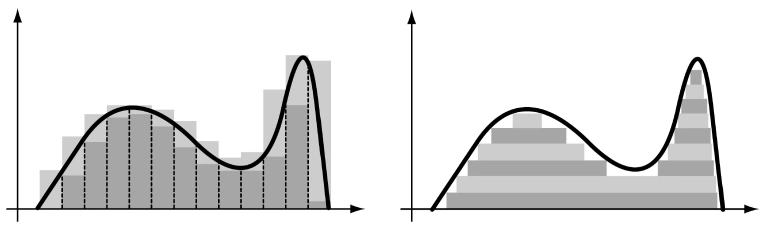
\includegraphics[width=0.75\linewidth]{img/riemann-vs-lebesgue.png}
 \vspace{0.5cm}
 \caption[Riemann and Lebesgue approximations]{Riemann and Lebesgue approximations \cite{schilling2017measures}}
 \label{figure:schilling}
\end{figure}

$$L_k^n=\{x\in\KK \,|\, t_k^n\le f(x)\le t_{k+1}^n\}.$$

Then the following approximation is usable for the area bounded by $f(D), y=0, x=a$ and $x=b$ for $D=[a,b]$, which coincides with Riemann integral.

\begin{equation}
 \label{example:lebesgue-partition}
 I_n=\sum\limits_{k=0}^{m_n-1}(t_{k+1}-t_k)\lambda(L_k^n).
\end{equation}

The additional requirement is that each $L^n_k$ is Lebesgue measurable. In Riemann integral, the function $f$ is required to be discontinuous at finite number of points, which is less general than Lebesgue measurability. Furthermore, Equation \ref{example:lebesgue-partition} can be generalized for abstract set $\Omega$ rather than $\RR^d$, its $\sigma$-algebra $\F$ and a measure $\mu$. In such measure space $(\Omega, \F, \mu)$, we will formally construct the Lebesgue integral for each measurable function $f:\Omega\to\RR$. The idea is to approximate $f$ by the limit of a sequence of steps function $(f_n)_{n\in\NN}$.

\begin{definition}[Step function]
 Let $(\Omega, \F, \mu)$ be a measure space. A function $f:\Omega\to\RR$ is a \textbf{step function}\index{step function} if there exists $\{A_n\}_{n=1}^N\subset\Omega$ and $\{c_n\}_{n=1}^N\subset\RR$ such that
 \begin{equation}
  f(x)=\sum\limits_{i=1}^nc_i\mathbf{1}_{A_i}(x).
 \end{equation}
\end{definition}

\begin{proposition}
 \label{proposition:standard-representation-of-a-step-function}
 Let $(\Omega, \F, \mu)$ be a measure space. Let $f:\Omega\to(0,\infty)$ be a positive step function. Then there exists a disjoint family $\{A_n\}_{n=1}^N\subset\Omega$ of nonempty sets, and a distinct set $\{c_n\}_{n=1}^N$ of positive number, such that
 \begin{equation}
  f(x)=\sum\limits_{n=1}^Nc_n\mathbf{1}_{A_n}(x).
 \end{equation}
 Moreover, this representation is unique.
\end{proposition}
\begin{proof}
 If there exist non-disjoint $A_i$ and $A_j$, we rewrite
 $$c_i\mathbf{1}_{A_i}(x) + c_j\mathbf{1}_{A_j}(x) = c_i\mathbf{1}_{A_i\setminus A_j}(x) + (c_i+c_j)\mathbf{1}_{A_i \cap A_j}(x) + c_j\mathbf{1}_{A_j\setminus A_i}(x),$$
 to achieve a disjoint family.

 If there exist $c_i = c_j$, we rewrite
 $$c_i\mathbf{1}_{A_i}(x) + c_j\mathbf{1}_{A_j}(x) = (c_i+c_j)\mathbf{1}_{A_i}(x) + c_j\mathbf{1}_{A_j\setminus A_i}(x).$$

 Then the attained subset of $\RR$ is disjoint. Let us abuse the original notation
 $$f(x)=\sum\limits_{n=1}^N c_n\mathbf{1}_{A_n}(x)$$
 for this new representation. For each $A_n, n\in\{1,\ldots,N\}$, choose $x_n\in A_n$. We have $f(x_n) = c_n > 0$. Now, consider two such representations
 $$f(x)=\sum\limits_{n=1}^Nc_n\mathbf{1}_{A_n}(x) = \sum\limits_{m=1}^Md_m\mathbf{1}_{B_m}(x).$$

 If $\bigcup_{n=1}^N A_n\setminus \bigcup_{m=1}^M B_m \ne \varnothing$, taking an element $x_0$ in this difference yields a contradiction when computing $f(x_0)$. Therefore, $\bigcup_{n=1}^N A_n\setminus \bigcup_{m=1}^M B_m = \varnothing$. Similar argument shows that $\bigcup_{n=1}^N A_n = \bigcup_{m=1}^M B_m$. Hence, for each $A_n, n\in\{1,\ldots, N\}$, there exists $B_m$ where $m\in\{1,\ldots,M\}$ such that $A_n\cap B_m\ne \varnothing$. Take $x_1\in A_n\cap B_m$, we have $f(x_1) = c_n = d_m$. If $A_n\setminus B_m \ne \varnothing$, take $x_2$ in this difference, then $f(x_2) = c_n = d_k$ for some $k\in\{1,\ldots,M\}$, a contradiction to the fact that $\{d_m\}$ is disjoint. Therefore, $A_n = B_m$. Thus, the representation is unique.
\end{proof}
\begin{remark}
 The representation in Proposition \ref{proposition:standard-representation-of-a-step-function} is called the standard representation. We can check that each positive step function $f$ has the standard representation
 \begin{equation}
  f(x) = \sum\limits_{t\in f(\Omega)} t\mathbf{1}_{\{x\in \Omega : f(x) = t\}}(x).
 \end{equation}
 If $f = 0, a.e.$, we choose the representation $f(x) = 0\cdot \mathbf{1}_{\Omega}(x)$. Let us denote by $\S^+$ the set of nonnegative step functions.
\end{remark}

\begin{corollary}
 Let $(\Omega, \F, \mu)$ be a measure space. Let $f:\Omega\to\RR$ be a step function. Then there exist a unique pair $f^+, f^-\in \S^+$ such that $f = f^+ - f^-$.
\end{corollary}

\begin{definition}[Lebesgue Integral of a Step Function]
 Let $(\Omega,\F,\mu)$ be a measure space and $f(x)=\sum\limits_{i=1}^nc_i\mathbf{1}_{A_i}(x)$ be a step function. The Lebesgue integral of $f$ with respect to a measure $\mu$ is defined as
 $$\int_\Omega f \d \mu = \sum\limits_{i=1}^nc_i\mu(A_i).$$
\end{definition}

We can see that the Lebesgue integral of a step function $f$ whose value coincides with the Riemann integral of $f$.

\begin{proposition}
 \label{proposition:integral-of-almost-everywhere-equal-step-functions}
 Let $(\Omega, \F, \mu)$ be a measure space and $f\in\S^+$. Suppose that $\Omega = E\cup E^c$, where $\mu(E^c) = 0$. Define a function $\tilde{f}:\Omega\to\RR$ as
 $$\tilde{f}(x) =\begin{cases}
   f(x), & \text{ if } x\in E    \\
   a,    & \text{ if } x\in E^c.
  \end{cases}$$
 Then $\int_\Omega f \d \mu = \int_\Omega \tilde{f} \d \mu$.
\end{proposition}

\begin{proof}
 We have
 \begin{align*}
  \int_\Omega \tilde{f} \d \mu
   & = \sum\limits_{t\in \tilde{f}(\Omega)} t\mu\left(\{x\in \Omega : \tilde{f}(x) = t\}\right)                                                                                                \\
   & = \sum\limits_{t\in \tilde{f}(\Omega)} t\mu\left(\{x\in E : \tilde{f}(x) = t\}\right) + \underbrace{a\mu(E^c)}_{0}                                                                        \\
   & = \sum\limits_{t\in \tilde{f}(\Omega)} t\mu\left(\{x\in E : \tilde{f}(x) = t\}\right)                                                                                                     \\
   & = \sum\limits_{t\in \tilde{f}(\Omega)} t\mu\left(\{x\in E : \tilde{f}(x) = t\}\right) + \underbrace{\sum\limits_{t\in \tilde{f}(\Omega)} t\mu\left(\{x\in E^c : \tilde{f}(x) = t\}\right)
  }_{0}                                                                                                                                                                                        \\
   & = \sum\limits_{t\in \tilde{f}(\Omega)} t\left[\mu\left(\{x\in E : \tilde{f}(x) = t\}\right) + \mu\left(\{x\in E^c : \tilde{f}(x) = t\}\right)\right]                                      \\
   & \sum\limits_{t\in \tilde{f}(\Omega)} t\mu\left(\{x\in \Omega : \tilde{f}(x) = t\}\right)                                                                                                  \\
   & = \int_\Omega f \d \mu.
 \end{align*}
\end{proof}

\begin{definition}
 Let $f:\Omega\to[0,\infty)$ be measurable. The Lebesgue integral of $f$ is defined as
 \begin{equation}
  \int_\Omega f\d \mu = \sup\left\{\int\limits h\d \mu(h) : h\in\S^+, h\le f\right\}.
 \end{equation}
\end{definition}

\begin{definition}
 Let $f:\Omega\to\RR$ be measurable. Define $f^+(x) = \sup(f,0)$ and $f^-(x) = \sup(-f,0)$. The Lebesgue integral of $f$ is defined as
 \begin{equation}
  \int_\Omega f\d \mu = \int_\Omega f^+\d \mu - \int(-f^-)\d \mu
 \end{equation}
 Then $f$ is said to be integrable or summable if $\int_\Omega f\d \mu<\infty$.
\end{definition}

\begin{definition}
 Let $f:\Omega\to\RR$ be measurable and $E \in \F$. The integral of $f$ over $E$ is defined as
 \begin{equation}
  \int_E f\d \mu = \int_\Omega f\mathbf{1}_E\d \mu.
 \end{equation}
\end{definition}

\begin{remark}
 When $(\Omega, \F, \mu) = (\RR^d, \B{(\RR^d)}, \lambda)$, Lebesgue integral coincides with Riemann integral. In such case, we simply write
 \begin{equation}
  \int_B f\d\lambda = \int_B f(x)\d x, B\in\B(\RR^d).
 \end{equation}
\end{remark}

\begin{proposition}
 \label{proposition:integral-of-le-everywhere-functions}
 Let $(\Omega,\F,\mu)$ be a measure space. Let $f$ and $g$ be measurable functions such that $f\le g, \mu-a.e.$ Then
 \begin{equation}
  \int_\Omega f\d \mu \le  \int_\Omega g\d \mu.
 \end{equation}
\end{proposition}

\begin{proof}
 If $f\le 0  \le g, \mu-a.e.$, we can use step functions approximation to prove that $\int_\Omega f\d \mu \le 0 \le  \int_\Omega g\d \mu$. If $f\le g\le 0$, we will prove that $0\le \int_\Omega -g\d \mu \le \int_\Omega -f\d \mu$. Hence, let us consider the case $ 0  \le f\le  g, \mu-a.e.$ Denote $E = \{x\in \Omega : f(x) \le g(x)\}$, we have $\mu(E^c) = 0$. For a step function $h\in S^+$, define $\tilde{h}$ similarly as in Proposition  \ref{proposition:integral-of-almost-everywhere-equal-step-functions}. We have
 \begin{align*}
  \int_\Omega f\d \mu
   & = \sup\left\{\int_\Omega f\d \mu : h\in \S^+, h\le f\right\}                                  \\
   & = \sup\left\{\int_\Omega f\d \mu : \tilde{h}\in \S^+, \tilde{h}\le f \text{ on } E\right\}    \\
   & \le  \sup\left\{\int_\Omega f\d \mu : \tilde{h}\in \S^+, \tilde{h}\le g \text{ on } E\right\} \\
   & =  \sup\left\{\int_\Omega f\d \mu : \tilde{h}\in \S^+, h\le g\right\}                         \\
   & =  \int_\Omega g\d \mu.
 \end{align*}
\end{proof}

\begin{corollary}
 \begin{enumerate}[label=(\roman*), ref=(\roman*)]
  \item []
  \item If $f = g, \mu-a.e.$, then $\int_\Omega f\d \mu =  \int_\Omega g\d \mu$.
  \item If $\int_\Omega |f|\d \mu = 0$, then $f=0,\mu-a.e.$
 \end{enumerate}
\end{corollary}

\begin{proof}
 For statement (i), we have $f\le g$ and $g\le f$, $\mu$-a.e. The conclusion follows directly from Proposition \ref{proposition:integral-of-le-everywhere-functions}. For statement (ii), let $E = \{x\in\Omega : |f(x)| = 0\}$, we have
 \begin{align*}
  0
   & = \int_\Omega |f|\d \mu                    \\
   & = \int_E |f|\d \mu + \int_{E^c} |f|\d \mu  \\
   & = \int_{E^c} |f|\d \mu                     \\
   & \ge \int_{E^c} \inf\limits_{E^c} |f|\d \mu \\
   & = \inf\limits_{E^c} |f| \mu (E^c)          \\
   & \ge 0
 \end{align*}
 Thus, $\mu (E^c)=0$ or $f=0$, $\mu$-a.e.
\end{proof}

To conclude this discussion of Lebesgue integral, we introduce $L^p$ spaces, crucial Banach spaces in functional analysis, particularly relevant for theorems in stochastic processes.

\begin{definition}
 \label{definition:Lp-space}
 Let $(\Omega,\F,\mu)$ be a measure space and $p\ge1$. The $L^p := L^p(\mu)$ space includes every function $f:\Omega\to\RR^m$, such that
 $$\left(\int\limits_\Omega \|f\|^p_p\d \mu\right)^{1/p}<\infty.$$
\end{definition}

\begin{remark}
 We can also define $L^\infty$ space. However, in the scope of the project, let us focus on $L^2$ onward. Those keen on delving deeper can refer to popular textbooks on Measure Theory \cite{cohn2013measure} or Functional Analysis \cite{rudin1987functional}.
\end{remark}

\begin{theorem}
 \label{theorem:L2-is-Banach}
 The $L^2$ space in Definition \ref{definition:Lp-space} is a vector space. The function $\|\cdot\|_{L^2} : L^2\to\RR$ be defined by
 $$\|f\|_{L^2(\mu)}=\left(\int\limits_\Omega \|f(x)\|^2_2\d \mu\right)^{1/2}, \forall f\in L^2.$$
 is a norm in the $L^2$ space. Moreover, the normed space $(L^2, \|\cdot\|_{L^2})$ is Banach.
\end{theorem}

\begin{proof}
 Firstly, we prove that $L^2$ is a vector space. Let $f,g \in L^2$, it is sufficient to show that $f+kg\in L^2$, for $k\in\RR$. Indeed, we have
 \begin{align*}
  \left(\int\limits_\Omega \|f + kg\|^2_2\d \mu\right)^{1/2}
   & \le \left(\int\limits_\Omega \left(\|f\|^2_2 + k^2\|g\|^2_2\right)\d \mu\right)^{1/2}                               \\
   & = \left(\int\limits_\Omega \|f\|^2_2\d \mu\right)^{1/2}  + \left(k^2\int\limits_\Omega \|g\|^2_2\d \mu\right)^{1/2} \\
   & < \infty.
 \end{align*}
 Now we prove that $\|\cdot\|_{L^2}$ is a norm. Nonnegativity and homogeneity are straightforward. Note that the function
 $\langle \cdot, \cdot\rangle : L^2 \times L^2\to \RR$ defined by
 \begin{equation}
  \langle f,g \rangle = \int\limits_\Omega fg \d \mu, \forall f,g\in L^2
 \end{equation}
 is a dot product in $L^2$. Using Cauchy-Schwarz inequality for any $f,g\in L^2$, we have
 \begin{align*}
  \|f + g\|_{L^2}^2
   & = \int\limits_\Omega \|f + g\|^2_2\d \mu                                                                                                                             \\
   & = \int\limits_\Omega (\|f\|_2 +\|g\|_2)^2\d \mu                                                                                                                      \\
   & = \int\limits_\Omega \|f\|_2^2\d \mu + \int\limits_\Omega \|g\|_2^2\d \mu + 2\int\limits_\Omega \|f\|_2\|g\|_2\d \mu                                                 \\
   & \le  \int\limits_\Omega \|f\|_2^2\d \mu + \int\limits_\Omega \|g\|_2^2\d \mu + 2\left(\int\limits_\Omega \|f\|_2\d \mu \int\limits_\Omega \|g\|_2\d \mu\right)^{1/2} \\
   & = \left( \left(\int\limits_\Omega \|f\|_2\d \mu\right)^{1/2} + \left(\int\limits_\Omega \|g\|_2\d \mu\right)^{1/2} \right)^2                                         \\
   & = \left(\|f\|_{L^2} + \|g\|_{L^2}\right)^2.
 \end{align*}
 Thus, triangle inequality is also satisfied.

 Finally, we prove that $L^2$ is complete. Consider a sequence $(f_n)_{n=1}^\infty\subset L^2$ such that $\lim\limits_{n\to\infty}\|f-f_n\|_{L^2}$. We have $\|f\|_{L^2}\le \|f-f_n\|_{L^2} + \|f_n\|_{L^2}, \forall n\in \NN$. Therefore,
 $$\|f\|_{L^2} \le \lim\limits_{n\to\infty}\left(\|f-f_n\|_{L^2} + \|f_n\|_{L^2}\right) = \lim\limits_{n\to\infty} \|f_n\|_{L^2} < \infty.$$
\end{proof}


\section{Probability Theory}

Classical interpretation of probability was popular until the work of Kolmogorov in 1993 on the axiomatic probability theory \cite{kolmogorov2018foundations}. Let us take a look on classical probability theory. A random experiment is a well-defined procedure that produces an observable outcome that could not be perfectly predicted in advance. Let $\Omega$ be the set of outcomes. Let $(\omega_n)_{n=1}^N$ be the sequence of outcomes when repeating the experiment $N$ times. An event $E$ is defined as a set of some elements in $\Omega$. At the $n$-th experiment, where $n\in\{1,\ldots,N\}$, the event $E$ is said to happen if $\omega_n\in E$. Classical probability interprets the event $E$ has probability $p$ as when we repeat the experiment $N$ times, where $N$ is sufficient large, then the ratio of outcome included in $E$ over $N$ is approximately $p$. We can write this interpretation as a limit
$$\lim\limits_{N\to\infty}\dfrac{|\{\omega_n : \omega_n\in E, n\in\{1,\ldots,N\}\}|}{N} = p.$$

Classical probability theory faces difficulties in problems whose statement is ambiguous, such as Bertrand's paradox \cite{shackel2007bertrand}. Kolmogorov's axiomatic probability theory was developed from measure theory. It provides a model for each probability calculation problem. Moreover, the theory then built consistent formal constructions of probabilistic objects, such as random variables and stochastic processes.

\subsection{Probability Space}

\begin{definition}
 Let $(\Omega, \F)$ be a measurable space. A measure $\PP$ on $(\Omega, \F)$ is called a \textbf{probability measure}\index{probability measure} if $P(\Omega)=1$. The triplet $(\Omega, \F, P)$ is called a \textbf{probability space}\index{probability space}.
\end{definition}

\begin{example}
 One rolls a fair dice once. Let $\Omega=\{1,2,3,4,5,6\}$ be the set of possible outcomes. Using classical probability, one can compute probability of several events, such as
 \begin{itemize}
  \item The probability of receiving an odd-number face is $P(\{1,3,5\})=\dfrac{1}{2}$.
  \item The probability of receiving a face whose number is less that $3$ is $P(\{1,2\})=\dfrac{1}{3}$.
 \end{itemize}
 The probability space $(\Omega, \F, P)$ for this problem contains
 \begin{itemize}
  \item $\Omega=\{1,2,3,4,5,6\}$.
  \item $\F=2^\Omega$.
  \item $P(A)=\dfrac{|A|}{6},\forall A\in\F$, where $|A|$ is the number of elements in $A$.
 \end{itemize}
\end{example}

\begin{remark}
 By convention, for $A,B\in\F$, we usually write the joint probability
 $P(A\cap B)$ by $P(A,B)$.
\end{remark}

\begin{definition}
 \label{definition:property-almost-surely}
 Given a probability space $(\Omega, \F, \PP)$. A property $\P:\Omega\to\{0,1\}$ is said to hold \textbf{almost surely}\index{almost surely} with respect to $\PP$, abbreviated by $\PP$-a.s. if
 \begin{equation}
  \PP\left(\left\{\omega\in\Omega : \P(\omega)\right\}\right) = 1.
 \end{equation}
 If $\PP$ is clear, we can just say $\P$ a.s.
\end{definition}

\begin{remark}
 The definition implies
 $$P(A\cap B)=P(B|A)P(A)=P(A)P(B)$$
 and
 $$P(A|B)=\dfrac{P(A\cap B)}{P(B)}=\dfrac{P(A\cap B)}{P(B|A)}=P(A).$$
 One can also check that three formulas are equivalent. Any of them can be used to define independent events.
\end{remark}

\subsection{Random Variables}
A probability calculation problem can sometimes be solved using more than one probability space. Consider the following example.

\begin{example}
 \label{example:probability-space-map}
 Locate four students Adam, Ben, Cam and Don to four chairs $A,B,C$ and $D$ randomly. We can compute the probability that Adam sits on chair $A$ as one of the followings. The more complicated inference is that there are $4! = 24$ ways to locate the students, whereas there are $3! = 6$ locating ways such that Adam sits on chair $A$, so the probability is $\dfrac{6}{24}=\dfrac{1}{4}$. On the other hand, we can think more simply that there is no bias of any chair that Adam sits, so the probability that Adam sits on chair $A$ is $\dfrac{1}{4}$. The first probability space $(\Omega_1, \F_1, \PP_1)$ has $24$ outcomes, whereas the second one $(\Omega_2, \F_2, \PP_2)$ has $4$ outcomes.
\end{example}

The equivalence of two probability spaces in solving the problem suggests that there is a map from the probability space with larger sample space to the one with smaller sample space $X : \Omega_1 \to \Omega_2$ such that for any two semantic-equivalent events $E_1\in\F_1$ and $E_2\in\F_2$, we have $\PP_1(E_1) = \PP_2(E_2)$.

\begin{example}
 In Example \ref{example:probability-space-map}, denote by $(X,Y)$ the outcome that student $X$ sits on chair $Y$. For the first probability space, we have
 $$\Omega_1=\{
  ((\text{Adam}, A), (\text{Ben}, B), (\text{Cam}, C), (\text{Don}, D)),
  \ldots,
  ((\text{Adam}, D), (\text{Ben}, C), (\text{Cam}, B), (\text{Don}, D))\}$$
 and $P_1(E_1) = \dfrac{|E_1|}{|\Omega_1|}$ for any $E_1\subset \Omega_1$. While for the second probability space, we have
 $$\Omega_2=\{(\text{Adam}, A), (\text{Adam}, B), (\text{Adam}, C), (\text{Adam}, D)\}$$
 and $P_2(E_2) = \dfrac{|E_2|}{|\Omega_2|}$ for any $E_2\subset \Omega_2$.
 The map $X$ in this cased is defined as $X(((\text{Adam}, Y), \ldots)) = (\text{Adam}, Y)$, for any $Y\in\{A,B,C,D\}$.
\end{example}

It derives that such map $X : \Omega_2 \to \Omega_1$ is measurable. In general, such map $X$ is called a probability preserving map.

\begin{definition}
 Let $(\Omega_1, \F_1, \PP_1)$ and $(\Omega_2, \F_2, \PP_2)$ be probability spaces. A measurable map $X : \Omega_1 \to \Omega_2$ is said to be \textbf{probability preserving}\index{probability preserving map} if
 $$\PP_1(X^{-1}(E_2)) = \PP_2(E_2), \forall E_2 \in \F_2.$$
\end{definition}

\begin{theorem}
 \label{theorem:probability-measure-wrt-measurable-map}
 Let $(\Omega_1, \F_1, \PP_1)$ be a probability space and $(\Omega_2, \F_2)$ be a measurable space. For any measurable map $X : \Omega_1 \to \Omega_2$, there exists a probability measure $\PP_2$ such that $X$ is probability preserving.
\end{theorem}

\begin{proof}
 Since $X$ is measurable, for any $E_2 \in \F_2, \PP_1(X^{-1}(E_2))$. The measure $\P_2$ is established such that
 $$\PP_2(E_2) = \PP_1(X^{-1}(E_2)), \forall E_2 \in \F_2.$$
\end{proof}

For computational purposes, we select $\Omega_2$ to be a real vector space, $\F_2 = \B(\Omega)$. The map $X$ is then called a \textit{random variable}.

\begin{definition}
 \label{definition:random-variable}
 Let $(\Omega, \F, P)$ be a probability space. A function $X:\Omega\to\RR^d$ is called a $d$-dimensional \textbf{random variable}\index{random variable} if $X$ is $(\F,\B(\RR^d))$-measurable. If $X_1,\ldots, X_N$, where $N\ge 2$ are random variables, then $(X_1,\ldots,X_N)$ is called a \textbf{random vector}\index{random vector}.
\end{definition}


% New page if possible, don't let this Remark title alone
\begin{remark}
 \begin{enumerate}[label = (\roman*)]
  \item []
  \item When we mention a random variable $X$ without further specification, we implicitly assume the existence of a probability space $(\Omega, \F, \PP)$ such that $X$ is $\F$-measurable.
  \item If the range $X(\Omega)$ is countable, then $X$ is said to be a \textbf{discrete random variable}\index{discrete random variable}.
  \item As a consequence of Theorem \ref{theorem:probability-measure-wrt-measurable-map}, every random variable $X$ induces a probability measure $\PP_X: \B(\RR^d)\to\RR$ such that
        \begin{equation}
         \PP_X(B) = \PP(\{\omega\in\Omega : X(\omega)\in B\}),
        \end{equation}
        called the distribution\index{distribution} of $X$. We usually briefly write $P(X\in B):= \PP(\{\omega\in\Omega : X(\omega)\in B\})$.
 \end{enumerate}
\end{remark}

\begin{proposition}[A Random Vector is a Random Variable]
 The following functions $X_1,\ldots,X_d: \Omega\to\RR$ are random variables if and only if the function $Y=(X_1,\ldots, X_d)$ defined by
 $$Y(\omega) = (X_1(\omega),\ldots, X_d(\omega)), \forall \omega\in\Omega$$
 is a random variable.
\end{proposition}

\begin{proof}
 Suppose that $X_1,\ldots,X_d$ are random variables, then
 $$X_i^{-1}((-\infty, b])\in \F, \forall b\in \RR, i\in \{1,\ldots,d\}.$$

 Therefore,
 \begin{align*}
  Y^{-1}(\{(x_1,\ldots,x_d): x_1\le b_1,\ldots, x_d\le b_d\})
   & = \bigcap\limits_{i=1}^d X_i^{-1}((-\infty, b_i]) \in \F, \forall b_1,\ldots,b_d\in \RR.
 \end{align*}
 Thus, $Y$ is a random variable. Conversely, suppose that $Y$ is a random variable, we have
 \begin{align*}
  X_i^{-1}((-\infty, b_i])
   & = X_i^{-1}((-\infty, b_i]) \cap \Omega                                                                                                 \\
   & = X_i^{-1}((-\infty, b_i]) \cap \left(\bigcap\limits_{j\ne i}^d X_j^{-1}(\RR)\right)                                                   \\
   & = Y^{-1}\left(\{(x_1,\ldots, x_d) : x_i \le b_i \text{ and } x_j \in \RR, \forall j\ne i\}\right) \in \F, \forall i\in\{0,\ldots, d\}.
 \end{align*}
 Thus, each $X_i$ where $i\in\{0,\ldots, d\}$ is a random variable.
\end{proof}

\begin{definition}
 Let $(\Omega, \F, P)$ be a probability space and $X:\Omega\to\RR^d$ be a random variable. Then
 $$\sigma(X)=\{X^{-1}(B) : B\in \B\}$$
 is called the $\sigma$-algebra generated\index{generated $\sigma$-algebra} by $X$ (See Proposition \ref{preposition:preimage-of-a-measurable-map-over-the imaged-sigma-algebra-is-a-sigma-algebra} that $\sigma(X)$ is indeed a $\sigma$-algebra). The $\sigma$-algebra generated by a random variable $X$ is interpreted as containing on information relevant to $X$.
\end{definition}

\begin{definition}
 Let $(\Omega, \F, P)$ be a probability space and $X:\Omega\to\RR^n$ be a random variable. Then the vector in $\RR^n$
 \begin{equation}
  \EE[X]=\int_{\Omega}X\d\PP=\int_{\RR^n}x\d \PP_x
 \end{equation}
 is called the \textbf{expectation}\index{expectation} of $X$.
\end{definition}

With the notion of expectation, we can restate the $L^2$ space for random variables as
\begin{equation}
 L^2(\PP) = \left\{X : \EE[\|X\|_2^2] < \infty \right\}.
\end{equation}

\begin{definition}
 Let $X$ be a $d$-dimensional random variable. If there exists a function $p_X:\RR^n\to [0,1]$ such that
 \begin{equation}
  \label{equation:density}
  \PP(X\in B)=\int_B p_X(x)\d \xbf, \forall B\in \B(\RR^d)
 \end{equation}
 then $X$ is said to be absolutely continuous\index{absolutely continuous}. We call $p_X$ the \textbf{probability density function}\index{probability density function} (PDF) of $X$, and denote by $X\sim p_X$.
\end{definition}

\begin{remark}
 Using Proposition \ref{proposition:equivalent-borel-core}, the condition (\ref{equation:density}) is equivalent to
 \begin{equation}
  \PP(x_1\le b_1, \ldots, x_n\le b_n)=\int\limits_{-\infty}^{b_d}\ldots\int\limits_{-\infty}^{b_1} p_X(x_1,\ldots,x_d)\d x_1\ldots\d x_d, \forall (b_1,\ldots,b_d)\in \RR^d.
 \end{equation}
 Therefore, in later proofs we will simply take the integral in Borel sets $B=\{(x_1,\ldots,x_d): x_i\le b_i, i=1,\ldots,d\}$.
\end{remark}

\begin{example}
 A ubiquitous distribution used probability theory and statistics is the Gaussian distribution $\N(\bm{\mu}, \Sigma)$. The normal density is given by
 \begin{equation}
  \N(\xbf;\bm{\mu}, \Sigma) := \N(\bm{\mu}, \Sigma)(\xbf) = \dfrac{1}{\sqrt{(2\pi)^d\det(\Sigma)}}\exp\left\{-\dfrac{1}{2}(\xbf-\bm{\mu})(\xbf-\bm{\mu})^\top\right\}.
 \end{equation}
\end{example}

\begin{remark}
 When we say $\{\xbf_n\}_{n=1}^N$ is sample from a PDF $p_X$, we mean that
 $$\lim\limits_{N\to\infty}\dfrac{|\{n: \xbf_n\in B\}|}{N} = \int\limits_{B}p_X(\xbf)\d\xbf,$$
 for any $B\in\B(\RR^d)$.
\end{remark}

If a random variable $X$ is discrete, then the function $p_X:\RR^d\to[0,1]$, such that $p_X(x) = \PP_X(x)$ is called the probability mass function (PMF) of $X$. Discreteness and absolute continuity are two extreme class of random variables. In such cases, the probability density function or mass function, if exists, contains all information about $X$. We do not concern discrete random variables in our scope. For absolutely continuous random variables, we define the joint density and the marginal density as an analogy to events.

\begin{definition}
 Let $X:\Omega\to\RR^{d_X}$ and $Y:\Omega\to\RR^{d_Y}$ are absolutely continuous random variables with density $p_X$ and $p_Y$, respectively. A function $p_{XY}:\RR^{d_X}\times \RR^{d_Y}\to[0,1]$ is called the \textbf{joint PDF}\index{joint PDF} if
 \begin{equation}
  \int_B\int_{A}p_{XY}(x,y)\d\xbf\d\ybf = \PP(\xbf\in A, \ybf\in B),\forall A\in\B(\RR^{d_X}), B\in\B(\RR^{d_Y}).
 \end{equation}
 A function $p_{X|Y}:\RR^{d_X} \times \RR^{d_y} \to[0,1]$ is called a \textbf{conditional PDF}\index{conditional PDF} if
 \begin{equation}
  \int_B \int_{A}p_{X|Y}(x, y) p_Y(y) \d\xbf \d\ybf  = \PP(\xbf\in A , \ybf\in B), \forall A\in\B(\RR^{d_X}), B\in\B(\RR^{d_Y}).
 \end{equation}
\end{definition}

\begin{theorem}[Algebra of density functions]
 \label{theorem:algebra-of-density-functions}
 Let $X$ and $Y$ be random variables with PDFs $p_X$ and $p_X$, respectively.
 \begin{enumerate}[label=(\roman*), ref=(\roman*)]
  \item The joint PDF of $X$ and $Y$ is given by
        \begin{equation}
         p_{X,Y}(x,y)=\dfrac{\partial^2 P_{X,Y}(x,y)}{\partial x\partial y},
        \end{equation}
        where $P_{X,Y}$ be the CDF of the random variable $(X,Y)$.
  \item Assume that $p_Y$ takes only positive values. The conditional PDF of $X$ given $Y$ is
        \begin{equation}
         p_{X|Y}(x,y)=\dfrac{p_{X,Y}(x,y)}{p_Y(y)}.
        \end{equation}
 \end{enumerate}
\end{theorem}
\begin{proof}
 Consider
 $$A=\{(x_1,\ldots,x_d): x_i\le a_i, i=1,\ldots,d\} \text{ and } B=\{(x_1,\ldots,x_d): x_i\le b_i, i=1,\ldots,d\}.$$
 The proof is derived from the Fundamental Theorem of Calculus.
\end{proof}

\begin{remark}
 If there is no ambiguity, we usually abbreviate the expressions
 $$p_{X,Y}(x\in A,y\in B) := p(x\in A,y\in B) \text{ and } p_{X|Y}(x\in A,y\in B) := p(x\in A|y\in B).$$
\end{remark}

Along with equality and convergence defined in $L^2$ space, almost sure equality and convergence are applicable for random variables as a stronger comparing criterion.

\begin{definition}
 Let $(\Omega, \F, P)$ be a probability space. Two random variables $X$ and $Y$ are said to be equal almost surely if
 $$\PP(\{\omega\in\Omega : X(\omega)=Y(\omega)\})=1,$$
 denoted by $X=Y, \,\,a.s.$
\end{definition}

\begin{definition}
 Let $(\Omega, \F, P)$ be a probability space. A sequence $(X_n)_{n\in \NN}$ of random variables is said to converge almost surely to a random variable $X$ if
 $$\PP\left(\left\{\omega\in\Omega : \lim\limits_{n\to\infty}X_n(\omega)=X(\omega)\right\}\right)=1.$$
\end{definition}

We can approximate how two random variables $X$ and $Y$ behave similarly to each other by their PDFs. In such case, we define a divergence\index{divergence}. A divergence is not a metric, but it gives more information than equality in distribution. Here we introduce the popular Kullback–Leibler divergence, which used in diffusion models (see Section \ref{section:diffusion-models}).

\begin{definition}
 \label{definition:KL-divergence}
 Let $P,Q$ be distribution functions. Assume that the corresponding densities $p$ and $q$ exist. The \textbf{Kullback–Leibler divergence}\index{Kullback–Leibler divergence} from $P$ to $Q$ is defined as
 \begin{equation}
  D_{\mathrm{KL}}(P\|Q) = \int_{\RR^d} p(x)\ln\dfrac{p(x)}{q(x)}\d x.
 \end{equation}
\end{definition}

\begin{remark}
 We can check that $D_{\mathrm{KL}}(P\|Q)\ge0$ with equality holds if $p=q$. In general, KL divergence is not symmetric i.e. $D_{\mathrm{KL}}(P\|Q)\ne D_{\mathrm{KL}}(Q\|P).$ Each expression serves a different purpose \cite{bishop2006pattern}.

 The symmetrized version developed from KL divergence called Jensen-Shannon (JS) divergence is also applicable
 \begin{equation}
  D_{\mathrm{JS}}(P\|Q) = \dfrac{1}{2}\left(D_{\mathrm{KL}}(P\|Q) + D_{\mathrm{KL}}(Q\|P)\right).
 \end{equation}
\end{remark}

\begin{example}
 Let $P:\left(a:\dfrac{3}{5}, b:\dfrac{1}{5}, c:\dfrac{1}{5}\right)$ is a categorical distribution. Here we mean that $P(x=a)=\dfrac{3}{5}$ and so on. Also let $Q:\left(a:\dfrac{1}{9}, b:\dfrac{4}{9}, c:\dfrac{4}{9}\right)$. Then
 $$D_{\mathrm{KL}}(P\|Q)=\dfrac{3}{5}\ln\left(\dfrac{3}{5}\cdot \dfrac{1}{9}\right)+\dfrac{1}{5}\ln\left(\dfrac{1}{5}\cdot \dfrac{4}{9}\right)+\dfrac{1}{5}\ln\left(\dfrac{1}{5}\cdot \dfrac{4}{9}\right)\approx 0.692,$$
 $$D_{\mathrm{KL}}(Q\|P)=\dfrac{1}{9}\ln\left(\dfrac{1}{9}\cdot \dfrac{3}{5}\right)+\dfrac{4}{9}\ln\left(\dfrac{4}{9}\cdot \dfrac{1}{5}\right)+\dfrac{4}{9}\ln\left(\dfrac{4}{9}\cdot \dfrac{1}{5}\right)\approx 0.522.$$
\end{example}

\begin{example}
 Let $p=\N(0,1)$ and $q=\N(1,1)$. Then
 \begin{align*}
  D_{\mathrm{KL}}(P\|Q)
   & =\int\limits_{-\infty}^\infty p(x)\ln\dfrac{p(x)}{q(x)}\d x                                                                                                                                                                \\
   & =\int\limits_{-\infty}^\infty \dfrac{1}{\sqrt{2\pi}}\exp\left\{-\dfrac{1}{2}x^2\right\}\ln\dfrac{\frac{1}{\sqrt{2\pi}}\exp\left\{-\frac{1}{2}x^2\right\}}{\frac{1}{\sqrt{2\pi}}\exp\left\{-\frac{1}{2}(x-1)^2\right\}}\d x \\
   & =\int\limits_{-\infty}^\infty \dfrac{1}{\sqrt{2\pi}}\exp\left\{-\dfrac{1}{2}x^2\right\}\left(-\dfrac{1}{2}x^2+\dfrac{1}{2}(x-1)^2\right)\d x                                                                               \\
   & =\int\limits_{-\infty}^\infty \dfrac{1}{2\sqrt{2\pi}}\exp\left\{-\dfrac{1}{2}x^2\right\}\left(1-2x\right)\d x                                                                                                              \\
   & =\dfrac{1}{2}\int\limits_{-\infty}^\infty\dfrac{1}{\sqrt{2\pi}}\exp\left\{-\dfrac{1}{2}x^2\right\}\d x-\dfrac{1}{\sqrt{2\pi}}\int\limits_{-\infty}^\infty\exp\left\{-\dfrac{1}{2}x^2\right\}\cdot x\d x                    \\
   & =\dfrac{1}{2},
 \end{align*}
 since $\exp\left\{-\dfrac{1}{2}x^2\right\}\cdot x$ is an odd function.
\end{example}

\subsection{Independence of Events and Random Variables}
\begin{definition}[Independent Events]
 Let $(\Omega, \F,\PP)$ be a probability space. Two events $A,B\in\F$ are said to be independent if
 \begin{equation}
  \PP(A \cap B)=\PP(A)\PP(B).
 \end{equation}
\end{definition}

\begin{theorem}[Conditional probability measure]
 Let $(\Omega, \F,\PP)$ be a probability space and an event $E\in\F$ such that $\PP(E)>0$. Define a function $\PP(\cdot|E):\F\to\RR$ as
 \begin{equation}
  \PP(X|E) = \dfrac{\PP(X\cap E)}{\PP(E)}
 \end{equation}
 Then $\PP(\cdot|E)$ is a probability measure, called $\PP(\cdot|E)$ the probability conditioned on an event $E$.
\end{theorem}

\begin{proof}
 For any $X\in\F$, we have $X\cap E\subset X$. Hence, $P(X,A)\le P(A)$, implying that $0\le P(X|A)\le 1.$

 On the other hand,
 $$\PP(\varnothing | E)=\dfrac{P(\varnothing\cap E)}{\PP(E)} = \dfrac{P(\varnothing)}{\PP(E)}=0 \text{ and } \PP(\Omega | E) =\dfrac{P(\Omega\cap E)}{\PP(E)} = \dfrac{\PP(E)}{\PP(E)} = 1.$$

 Finally, for a pairwise disjoint collection $\{X_i\}_{i=1}^\infty$, the collection $\{X_i\cap A\}_{i=1}^\infty$ is also pairwise disjoint. Therefore,
 \begin{align*}
  \sum\limits_{i=1}^\infty P(X_i|A)
   & = \dfrac{1}{P(A)}\sum\limits_{i=1}^\infty P(X\cap A)                  \\
   & =\dfrac{1}{P(A)}P\left(\bigcup\limits_{i=1}^\infty (X_i\cap A)\right) \\
   & =\dfrac{1}{P(A)}P\left(\bigcup\limits_{i=1}^\infty X_i \cap A \right) \\
   & = P\left(\bigcup\limits_{i=1}^\infty X_i|A\right).
 \end{align*}
 Thus, $\PP(\cdot|E)$ is a probability measure.
\end{proof}

\begin{remark}
 One can check that the independence between events $A$ and $B$ can be equivalently defined by one of the following formulas
 \begin{enumerate}[label=(\arabic*)]
  \item $\PP(A \cap B)=\PP(A)\PP(B)$,
  \item $\PP(A | B)=\PP(A)$,
  \item $\PP(B | A)=\PP(B)$.
 \end{enumerate}
\end{remark}

\begin{definition}
 Two random variables $X:\Omega\to\RR^{d_X}$ and $Y:\Omega\to\RR^{d_Y}$ are said to be independent if
 \begin{equation}
  \label{definition:independent-random-variables}
  \PP(X\in B_X, Y\in B_Y)=\PP(X\in B_X)\PP(Y\in B_Y), \forall B_X\in\B(\RR^{d_X}), B_Y\in\B(\RR^{d_Y}).
 \end{equation}
\end{definition}

\begin{proposition}
 Let $X:\Omega\to\RR^{d_X}$ and $Y:\Omega\to\RR^{d_Y}$ be absolutely continuous random variables. Then $X$ and $Y$ are independent if either
 \begin{enumerate}[label=(\arabic*)]
  \item $p_{XY}=p_Xp_Y$,
  \item $p_{X|Y}=p_X$,
  \item $p_{Y|X}=p_Y$.
 \end{enumerate}
\end{proposition}

\begin{proposition}
 \label{theorem:independent-expectation}
 Let $X$ and $Y$ be absolutely continuous $L^1$ real-value random variables. If $X$ and $Y$ are independent, then
 \begin{equation}
  \EE[XY]=\EE[X]\EE[Y].
 \end{equation}
\end{proposition}

\begin{proof}
 We have
 \begin{align*}
  \EE[XY]
   & = \int_{\RR}\int_{\RR}p_{X,Y}(x,y)\d x\d y  \\
   & = \int\_{\RR}\int_{\RR}p_X(x)p_Y(y)\d x\d y \\
   & =\int_{\RR}p_X(x)\d x\int_{\RR}p_Y(y)\d y   \\
   & =\EE[X]\EE[Y].
 \end{align*}
\end{proof}

\subsection{Conditional Expectations}
The concept of conditional expectations generalizes the study of expectation and independence.

\begin{definition}[Expectation Conditioned on an Event]
 Let $(\Omega, \F,\PP)$ be a probability space and an event $E\in\F$. The conditional expectation of $X$ given $E$ is defined as
 \begin{equation}
  \EE(X|E)=\int_{E}X\d \PP(X|E).
 \end{equation}
\end{definition}

\begin{example}
 Three coins, 10p, 20p and 50p are tossed. The values of those coins that land heads up are added to work out the total amount $X$. Calculate the expected total amount given that two coins have landed heads up.
\end{example}

\begin{solution}
 Let $E$ denote the even that two coins have landed heads up, then $E=\{HHT, HTH, THH\}$. Each element has the same probability of $\dfrac{1}{8}$ so $P(E)=\dfrac{3}{8}$. Therefore,

 $$P(X|E)=\dfrac{1}{P(E)}\left(\dfrac{1}{8}(10+20)+\dfrac{1}{8}(10+50)+\dfrac{1}{8}(20+50)\right)=53\dfrac{1}{3}.$$
\end{solution}

The expectation conditioned on a random variable and the expectation conditioned on a $\sigma$-algebra is closely related. Intuitively, let $X$ and $Y$ be random variables. The expectation of $X$ given $Y$ is a random variable $Z := \EE[X|Y]$ such that $\EE[Z]$ is the best guess for the value of $X$ given all possible occurrences of $Y$. However, formal definition of $\EE[X|Y]$ concerns about $\sigma(Y)\subset\F$. Generally, consider a sub-$\sigma$-algebra $\G$ of $\F$. Because $X$ may not be $\G$-measurable, when just looking at $\G$, we may lack information about $X$. The expectation of $X$ given $\G$ is thought of as a random variable $T:= \EE[X|\G]$ such that $\EE[T]$ is the best guess for the value of $X$ when seeing $\G$.

\begin{definition}[Expectation Conditioned on a $\sigma$-algebra]
 Let $(\Omega, \F, \PP)$ be a probability space and $\G$ be a sub-$\sigma$-algebra of $\F$. The conditional expectation a random variable of $X$ conditioned on $\G$ is a $\G$-measurable random variable $\EE(X|\G)$ such that
 \begin{equation}
  \int_A \EE(X|\G)\d \PP=\int_A X\d \PP, \forall A\in\G.
 \end{equation}
\end{definition}

\begin{definition}[Expectation Conditioned on a Random Variable]
 Let $(\Omega, \F, \PP)$ be a probability space and $X,Y$ be random variables. The expectation of $X$ conditioned on $Y$ a $\sigma(Y)$-measurable random variable $\EE(X|Y)$ such that
 \begin{equation}
  \int_A \EE(X|Y)\d \PP = \int_A X\d \PP, \forall A\in\sigma(Y).
 \end{equation}
\end{definition}

The next theorem indicates that the conditional expectation depends only on the $\sigma$-algebra generated by a random variable, but not the random variable itself.

\begin{theorem}
 Let $Y,Z$ be random variables such that $\sigma(Y)=\sigma(Z)$. Then for any random variable $X$,
 $$\EE(X|Y)=\EE(X|Z),\,\,a.s.$$
\end{theorem}

\begin{proof}
 Let $\G=\sigma(Y)=\sigma(Z)$. For any $B\in\G$, we have

 $$ \int_B X\d P=\int_B \EE(X|Y)\d P=\int_B \EE(X|Z)\d P.$$

 Let $T=\EE(X|Y)-\EE(X|Z)$, we have

 $$\int_B T\d P = 0,\,\,\forall B\in\G.$$

 We will prove that $T=0 \,\,a.s.$ For any $\epsilon>0$,

 \begin{align*}
  0\ge\epsilon P(T\ge \epsilon) =\int_{T\ge\epsilon}\epsilon\d P\ge \int_{T\ge\epsilon}X\d P=0.
 \end{align*}

 The last equality holds since $\{T\ge\epsilon\}\in\G$. Hence, $P(T\ge \epsilon)=0$. Similarly, $P(T\le -\epsilon)=0$. Therefore,

 $$P(-\epsilon < T <\epsilon) = P(|T|<\epsilon) = 1.$$

 By letting $\epsilon\to 0$, we conclude that $T=0\,\,a.s.$ Thus, $\EE(X|Y)=\EE(X|Z),\,\,a.s.$
\end{proof}

% \begin{theorem}
%   Let $(\Omega, \F, \PP)$ be a probability space. If $X,Y$ are integrable real-valued random variables, then
%   $\EE[XY] = \EE[X]\EE[Y]$.
% \end{theorem}
% \begin{proof}

% \end{proof}
\section{Stochastic Processes}
\label{subsection:stochastic-processes}
There are real-life problems where we consider the evolution of a phenomenon overtime. For example, let $N_0$ be the original number of bacterial cells in the population. The number of bacteria in a population at time $t$ is can be modeled by
\begin{equation}
  \label{example:bacterial-growth}
  N_t = N_0\times 2^t.
\end{equation}

Such model is said to be deterministic. For other problems, such as the evolution of the stock price overtime, deterministic models are not a good selection, since we have to express the risk carefully for every decision on the market. Therefore, randomness should be concerned. In such cases, instead of using such deterministic equation as \ref{example:bacterial-growth}, we allow our equation results in random variables. Hence, we can compute a collection $\{X_t\}_{t\ge0}$ of random variables, which is called a stochastic process.

\subsection{Definitions}

\begin{definition}
  \label{definition:stochastic-process}
  A collection of random variables $\{X_t\}_{t\in I}$ on the same probability space $(\Omega,\F, P)$ is called a stochastic process. For each fixed point $\omega_0\in\Omega$, the map $t\mapsto X(\omega_0, t)$ is called a sample path.
\end{definition}

\begin{remark}
  We can regard a stochastic process as function of two parameters
  $$X:I\times\Omega \to \RR^d.$$
  Hence, sometimes we write $X(t,\omega)$ instead of $X_t(\omega)$. In this case, we assume that $X$ is ($\F\otimes\B(I),\B(\RR^n)$)-measurable.
\end{remark}

\begin{definition}
  Let $\{X_t\}_{t\in I}$ be a stochastic process. If the index set $I$ is countable, then $\{X_t\}_{t\in I}$ is called a discrete-time stochastic process. If $I$ is an interval of $\RR$, then $\{X_t\}_{t\in I}$ is called a continuous-time stochastic process.
\end{definition}

\begin{remark}
  Without loss of generality, if $\{X_t\}_{t\in I}$ is discrete-time, we can choose $I = \NN$, if $\{X_t\}_{t\in I}$ is continuous-time, we will choose $I=\RR$. These selections of the index set are applied for later statements.
\end{remark}

Recall that the $\sigma$-algebra generated by a random variable $X$ is thought of as containing all information about $X$. When a stochastic process evolves overtime, our knowledge about the process increase. For a time $t\in I$, this cumulative information is encapsulated in a $\sigma$-algebra such that all previous random variables $\{X_s\}_{s\in I, s\le t}$ are measurable.

\begin{definition}
  Let $(\Omega, \F, \PP)$ be a probability space. A increasing family $\{\F_t\}_{t\in I}$ of sub-$\sigma$-algebras of $\F$ i.e.
  $$\F_s\subset\F_t \subset \F, \forall t\in I, s\le t$$
  is called a filtration. If
  $$\F_t = \bigcap\limits_{r\ge t} \F_r,$$
  then $\{\F_t\}_{t\in I}$ is said to be right-continuous.

  The tuple $(\Omega, \F, \{\F_t\}_{t\in I}, P)$ is called a filtered probability space.
\end{definition}

\begin{definition}
  Let $(\Omega, \F, \{\F_t\}_{t\in I}, P)$ be a filtered probability space. A stochastic process $\{X_t\}_{t\in I}$ is said to be adapted to the filtration $\{\F_t\}_{t\in I}$ if for any $t\in I$, each random variable $X_s$ where $s\le t$ is $\F_t$ measurable.
\end{definition}

\begin{theorem}
  Let $(\Omega, \F, \PP)$ be a probability space and $\{X_t\}_{t\in I}$ is a stochastic process. Then the family $\{\hat{\F}_t\}_{t\in I}$ of $\sigma$-algebras defined by
  $$\hat{\F}_t = \sigma\left(\left\{\bigcup\limits_{\substack{s\in I \\ s\le t}} \sigma(X_s)\right\}\right)$$
  is a filtration to which $\{X_t\}_{t\in I}$ is adapted. Moreover, the family $\{\hat{\F}_t\}_{t\in I}$ is the smallest adapting filtration i.e. if $\{X_t\}_{t\in I}$ is adapted to another filtration $\{\F_t\}_{t\in I}$, then
  $$\hat{\F}_t \subset \F_t, \forall t\in I.$$
  We called $\{\hat{\F}_t\}_{t\in I}$ the natural filtration \index{natural filtration} of $\{X_t\}_{t\in I}$.
\end{theorem}

We assert the equality of two random variables $X$ and $Y$ in the almost sure sense or in distribution. It is natural to extend this concept of equality to two stochastic processes $\{X_t\}_{t\in I}$ and $\{Y_t\}_{t\in I}$.

\begin{definition}
  Let $(\Omega, \F, \PP)$ be a probability space. Two stochastic processes $\{X_t\}_{t\in I}$ and $\{Y_t\}_{t\in I}$ are said to be indistinguishable \index{indistinguishable} if there exists $A\in\F$ with $P(A)=1$, such that for each
  $$X_t(\omega)= Y_t(\omega), \forall \omega\in A, t\in I.$$
\end{definition}

\begin{definition}
  Let $(\Omega, \F, \PP)$ be a probability space. Let $\{X_t\}_{t\in I}$ and $\{Y_t\}_{t\in I}$ be stochastic processes. We say that $\{X_t\}_{t\in I}$ is a version of $\{Y_t\}_{t\in I}$ if
  $$X_t=Y_t,\,\, a.s \,\,\,\,\forall t\in I.$$
\end{definition}

\begin{remark}
  We can check that ``is a version of'' is an equivalence relation.
\end{remark}

\begin{example}
  \label{example:dis}
  Let $\Omega=I=[0,1]$, $\F=\B(\Omega)$ and $T$ be a random variable distributed uniformly on $\Omega$, $X_t=\mathbf{1}_{t=T}$, then for each $t\in[0,1]$,

  $$P(X_t\ne 0) = P(t=T) = 0.$$

  However, $X_t$ is not indistinguishable from the constant process zero, since there is no subset $A$ of $\Omega$ with $P(A)=1$ such that for each $t\in I$, $X_t(\omega)= 0, \forall \omega\in A.$
\end{example}

For random variables, we adjust the $L^2$ norm in an $L^2$ space to study their convergence in a computationally efficient way. We also create a space $\L^2$ for stochastic processes such that they do not explode. Also, if a sequence $(\{X_n(t)\}_{t\in[0,T]})_{n\in\NN}$ of processes converges to $\{X(t)\}_{t\in[0,T]}$, then it guarantees that for each $t\in[0,T]$,
$$X_n(t) \xrightarrow{n\to\infty} X(t) \text{ in } L^p.$$

\begin{definition}[The $\L^2$ space of stochastic processes]
  Define $\L^2:=\L^2(\Omega, [0,T])$ to be the space of stochastic processes such that for each $\{X_t\}_{t\in [0,T]}\in \L^2$,
  $$\EE\left[\int\limits_0^T X^p_t \d t\right] < \infty.$$
\end{definition}


\begin{theorem}
  The function $\|\cdot\|_{\L^2}:\L^2\to\RR$ defined by
  \begin{equation}
    \|\{X_t\}_{t\in [0,T]}\|_{\L^2} = \left(\EE\left[\int\limits_0^T X^p_t \d t\right]\right)^{1/2}
  \end{equation}
  is a norm on $\L^2$, called the $\L^2$-norm. Moreover, the normed space $(\L^2, \|\cdot\|_{\L^2})$ is Banach.
\end{theorem}

% \begin{proof}

% \end{proof}

\subsection{Wiener Processes}

We introduce a popular stochastic process that appears in the Definition \ref{definition:sde} of a stochastic differential equation.

\begin{definition}
  \label{definition:wiener-process}
  A real-valued stochastic process $\{W_t\}_{t\ge0}$ is called the one-dimensional Wiener process or Brownian motion if
  \begin{enumerate}
    \item $W_0=0$ a.s.
    \item $W(t_2)-W(t_1) \sim \N(0,t-s)$.
    \item Independent increments: for any three times $t_1<t_2<t_3$, the random variables $W(t_2)-W(t_1)$ and $W(t_3)-W(t_2)$ are independent.
    \item The sample path $t\mapsto W(t,\omega)$  is continuous a.s.
  \end{enumerate}
  An $d$-dimensional Wiener process is a vector of $d$ one-dimensional Wiener processes.
\end{definition}

\begin{figure}
  \centering
  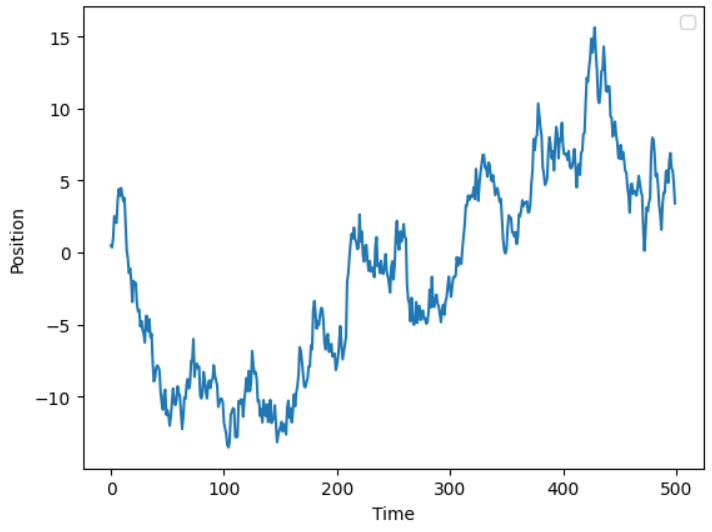
\includegraphics[width=0.5\linewidth]{img/1d-brownian.png}
  \vspace{0.5cm}
  \caption{An illustration of the Wiener process.}
  \label{figure:brownian-motion-illustration}
\end{figure}

\begin{theorem}[Quadratic Variation]
  \label{theorem:quadratic-variation}
  Let $[a, b]$ be an interval in $[0,\infty)$ and partitions
  $$P^n=\{0=t_0^n\le t_1^n\le\ldots\le t_m^n=T\},$$
  with $\left|P^n\right|\to0$ as $n\to\infty$. Then
  \begin{equation}
    \sum\limits_{k=0}^{m_n-1}\left(W\left(t_{k+1}^n\right)-W\left(t_k^n\right)\right)^2\to b-a
  \end{equation}
  as $n\to\infty$.
\end{theorem}

\begin{proof}
  Let $Q_n=\sum\limits_{k=0}^{m_n-1}\left(W\left(t_{k+1}^n\right)-W\left(t_k^n\right)\right)^2$, then
  $$Q_n-(b-a)=\sum\limits_{k=0}^{m_n-1}\left(\left(W\left(t_{k+1}^n\right)-W\left(t_k^n\right)\right)^2-\left(t^n_{k+1}-t^n_k\right)\right).$$

  Hence,
  \begin{align*}
     & \EE[(Q_n-(b-a))^2]                                                                                                                                                                                                                                                                           \\
     & =\sum\limits_{k=0}^{m_n-1}\sum\limits_{j=0}^{m_n-1}\EE  \left[\left(\left(W\left(t_{k+1}^n\right)-W\left(t_k^n\right)\right)^2-\left(t^n_{k+1}-t^n_k\right)\right)\right. \left.\left(\left(W\left(t_{j+1}^n\right)-W\left(t_j^n\right)\right)^2-\left(t^n_{j+1}-t^n_j\right)\right)\right].
  \end{align*}

  If $k\ne j$, due to independent increment, the term becomes the product of two expectations. Since $W(t)-W(s)\sim \N(0,t-s)$ for $t>s\ge 0$, the first expectation is

  $$\EE\left[\left(\left(W\left(t_{k+1}^n\right)-W\left(t_k^n\right)\right)^2-\left(t^n_{k+1}-t^n_k\right)\right)\right]=0.$$

  Therefore, this term vanishes and
  \begin{align*}
    \EE[(Q_n-(b-a))^2]=\sum\limits_{k=0}^{m_n-1}\EE\left[\left(\left(W\left(t_{k+1}^n\right)-W\left(t_k^n\right)\right)^2-\left(t^n_{k+1}-t^n_k\right)\right)^2\right].
  \end{align*}
  Let $Y_k = \dfrac{W\left(t_{k+1}^n\right)-W\left(t_k^n\right)}{\sqrt{t_{k+1}^n-t_k^n}}\sim\N(0,1)$, we have
  \begin{align*}
    \EE\left[\left(\left(W\left(t_{k+1}^n\right)-W\left(t_k^n\right)\right)^2-\left(t^n_{k+1}-t^n_k\right)\right)^2\right] & =\EE\left[(t^n_{k+1}-t^n_k)^2(Y_k^2-1)^2\right]  \\
                                                                                                                           & =(t^n_{k+1}-t^n_k)^2\EE\left[(Y_k^2-1)^2\right].
  \end{align*}
  Let $C=\max\limits_{i=1,\ldots,k}\left\{\EE\left[(Y_k^2-1)^2\right]\right\}$, we have

  $$\EE[(Q_n-(b-a))^2]\le C\sum\limits_{k=0}^{m_n-1}(t^n_{k+1}-t^n_k)^2\to 0 \text{ as } n\to\infty.$$
\end{proof}

Also, every stochastic process is associated with a class of its modifications, whose finite distributions are the same. We say that a stochastic process identifies a \textit{probability law}\index{probability law}. From now on, we denote $P^0$ the probability law of a process starting from time $0$.

\subsection{Markov Processes}

\begin{definition}[Markov Property]
  Let $(\Omega, \F, \PP)$ is a probability space. A stochastic process $\{M_t\}_{t\in[0,T]}$ adapted to a filtration $\{\F_t\}_{t\in[0,T]}$ is a Markov process if
  \begin{equation}
    \EE[M_t|\F_s] = \EE[M_t|M_s],  \forall 0 \le s \le t \le T.
  \end{equation}
  A Markov process is said to be time-homogeneous if $M_t = M_s, a.s.$ for some $t > s$ implies that $M_{t+r} = M_{s+r}, a.s. \forall r\ge0$.
\end{definition}

\begin{definition}[Infinitesimal Generator]
  Let $\{K_t\}$ be a continuous-time semigroup of linear operators on $L^2$. We say that a function $f\in L^2$ belongs to $\mathrm{Dom}(G)$ if the limit
  \begin{equation}
    \lim\limits_{h\downarrow 0}\dfrac{K_hf - K_0f}{h} := Gf
  \end{equation}
  exists in $L^2$. In such cases, $G$ is called the infinitesimal generator of $\{K_t\}$.
\end{definition}

\begin{theorem}[The Derivative of a Function Evolved by a Semi-Group]
  Let $G$ be the generator of a semigroup of linear operators $\{K_t\}$ on $L^2$. For a fixed $f\in\Dom(G)$, set $u(x,t) := (K_tf)(x)$. Then $\partial_t u$ exists for all $t$, and is equal to $Gu$.
\end{theorem}
% \begin{proof}

% \end{proof}

\begin{definition}[Self-space Markov Kernel]
  Let $(\Omega, \F)$ be a measurable space. A function $\kappa: \Omega\times\F\to[0,1]$ is called a (self-space) Markov kernel on $(\Omega, \F)$  if
  \begin{enumerate}[label=(\roman*), ref=(\roman*)]
    \item For any $F\in\F$, the function $\kappa(\cdot, F): \Omega \to [0,1]$ is $\F$-measurable.
    \item For any $\omega\in\Omega$, the function $\kappa(\omega, \cdot): \F\to [0,1]$ is a probability measure on $(\Omega, \F)$.
  \end{enumerate}
\end{definition}

\begin{definition}
  Let $(\Omega, \F)$ be a measurable space. Let $\kappa_1$ and $\kappa_2$ be Markov kernels. The product $\kappa_1\kappa_2 : \Omega \to \F$ is a Markov kernel, defined as
  \begin{equation}
    (\kappa_1\kappa_2)(x,F) = \int_{y\in\Omega}\kappa_2(y,F)\d\kappa_1(x,y).
  \end{equation}
\end{definition}

\begin{definition}[Transition Kernel]
  Let $(\Omega, \F)$ be a measurable space. For every $0\le s\le t\le T$, let $\kappa_{s,t}$ be a Markov kernel on $(\Omega, \F)$. The family $\{\kappa_{s,t}\}$ is called a semigroup of transition kernels if
  \begin{enumerate}[label=(\roman*), ref=(\roman*)]
    \item For any  $t$, $\kappa_{t,t}(x,B) = \delta_{B}(x)$.
    \item For any $0\le r\le s\le t\le T$, $\kappa_{r,t} = \kappa_{r,s}\kappa_{s,t}$.
  \end{enumerate}
\end{definition}

\begin{definition}
  Let $(\Omega, \F)$ be a measurable space and $\{\kappa_{s,t}\}$ is a semigroup of transition kernels. We define $\{K_{s,t}\}$ the semigroup of transition operators on $B(\RR^d,\RR)$ as
  \begin{equation}
    (K_{s,t}f)(x) = \int\limits_{y\in\Omega}f(y)\d \kappa(x,y) := \kappa_{s,t}(f(x)), \forall x\in\RR^d.
  \end{equation}
\end{definition}

\begin{theorem}[Transition Operator Semigroups and Markov Processes]
  Let $X$ be a Markov process with transition kernels $\{\mu_{s,t}\}$, and let $\{K_{s,t}\}$ be the corresponding semigroup of transition operators. Then for any $f \in B(\RR^d, \RR)$, we have
  \begin{equation}
    \label{equation:transition-operator-semigroups-and-markov-process}
    \EE[X_t | \F_s] = (K_{s,t}f)(X_s).
  \end{equation}
  Conversely, let $X$ be any stochastic process, and let $K_{s,t}$ be a semigroup of transition operators such that Equation \ref{equation:transition-operator-semigroups-and-markov-process} is valid (a.s.). Then $X$ is a Markov process.
\end{theorem}
\begin{proof}
  We have
  \begin{align*}
    (K_{s,t}f)(X_s)
     & = \int\limits_{y\in\Omega}f(y)\d \kappa_{s,t}(x,y) \\
     & = \E[f(X_t) | \sigma(X_s)]                         \\
     & = \EE[X_t | \F_s].
  \end{align*}
\end{proof}

\begin{definition}[Martingale Problem]
  Let $G$ be a generator on $\D\subset\C_b(\RR^d, \RR)$. A $d$-dimensional stochastic process $X:=\{X_t\}$ is a solution to the martingale problem for $G$, $\D$, if for any $f\in \D$,
  \begin{equation}
    f(X_t) - \int\limits_0^t Gf(X_s)\d s
  \end{equation}
  is a martingale with respect to ${\F^X_t}$, the natural filtration of X.
\end{definition}

\begin{lemma}
  A stochastic process $X:=\{X_t\}$ is a solution to the martingale problem if and only if
  \begin{equation}
    \EE\left[f(X_t)|\F^X_s\right] - \EE\left[\left.\int\limits_{s}^t Gf(X_r)\d r \right| \F^X_s\right] = f(X_s), \forall 0\le s\le t\le T.
  \end{equation}
\end{lemma}
% \begin{proof}

% \end{proof}

\begin{theorem}
  Let $X$ be a homogeneous Markov process with generator $G$ and cadlag sample paths. Then X solves the martingale problem for $G$, $\C_b(\RR^d, \RR)\cap \mathrm{Dom}(G)$.
\end{theorem}

\begin{definition}
  Let $(\Omega, \F)$ is a probability space. A function $\kappa: \F \times \RR \to [0,1]$ is called a probability kernel.
\end{definition}

\begin{definition}
  Let $\kappa_1$ and $\kappa_2$ be probability kernels. The product of $\kappa_1$ and $\kappa_2$ is defined as
  \begin{equation}
    (\kappa_1\kappa_2)(x, D) = \int\kappa_1(x, D)\d\kappa(x, y).
  \end{equation}
\end{definition}

\begin{definition}
  Let $\D$ be the set of all distributions on $\RR^d$. For every $s,t$, a probability kernel $\kappa_{s,t} : \D \times \D \to [0,1]$ is called a transition kernel if
  \begin{enumerate}[label = (\roman*)]
    \item For all $t\in[0,T]$ and $D\in\D$, $\kappa_{t,t}(D, ) = \mathbf{1}_{D}(\cdot)$.
    \item For any $r\le s\le t$, $\kappa_{r,t}=  \kappa_{r,s}\kappa_{s,t}$.
  \end{enumerate}
  We usually call $\{\kappa_{s,t}\}$ a transition semigroup.
\end{definition}

Each Markov process is associated with a transition semigroup. Conversely, given a transition semigroup, there exists a corresponding Markov process.


\section{Stochastic Integrals}
\label{subsection:stochastic-integrals}
\subsection{Motivation}
Suppose that we want to model the stock price where the time points are in the interval $[0,T]$. We firstly consider a discrete case where $T \in \NN$ and the intermediate time points are $t_n = n, n \in \{0,\ldots, T\}$. Let $p_0$ be the initial stock price at time $t_0$. We wish to establish the formula for the stock price at each time $t_n = n, n \in \{0,\ldots, T\}$ in a nondeterministic way, due to market uncertainty. We can instead formulate the evolution of the price over each time step. Let $\{X_n\}_{n=0}^T$ be a stochastic process where $X_n$ is the price at time $t_n=n$, we have

\begin{equation}
  \begin{cases}
    X_0= p_0 \\
    X_{n+1} - X_n = b(X_n,n) + \sigma(X_n,n)\cdot \texttt{noise}, \,\,\,n\in \{0,\cdots, T-1\},
  \end{cases}
\end{equation}

where $b,\sigma:\RR\times\NN\to\RR$. We select the standard normal random variable for this noise
$$\texttt{noise}:= Z_{n} = W_{n+1}-W_n \sim \N(0,1),$$

by which we hypothesized that if the noise acts more complicatedly, then we can adjust $\sigma(X_n,n)$ to be $\hat{\sigma}(X_n,n)$ such that
$$\sigma(X_n,n)\cdot \texttt{noise} = \hat{\sigma}(X_n,n)(W_{n+1}-W_n) \text{ in } L^2.$$

Our reasonable model is
\begin{equation}
  \label{example:stock-price}
  \begin{cases}
    X_0= p_0 \\
    X_{n+1} - X_n = b(X_n,n) + \sigma(X_n,n)\cdot Z_{n}, \,\,\,n\in \{0,\cdots, T-1\},
  \end{cases}
\end{equation}

\begin{figure}
  \centering
  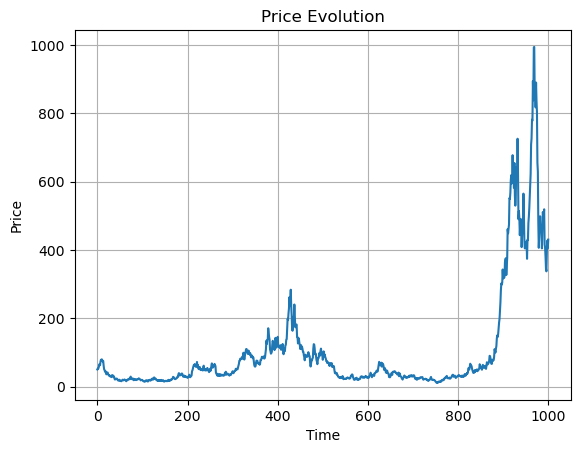
\includegraphics[width=0.7\textwidth]{img/stock-price-sampling.png}
  \vspace{0.25cm}
  \caption[Stock price simulation]{A simulation of stock price evolution by $X_{n+1} - X_n = rX_n + \alpha X_n\cdot Z_{n}$, where $p_0=50, r = 0.005
      \alpha = 0.1$}
\end{figure}

By using time discretization, when it requires to estimate the price at non-integer time, say $t=n+\dfrac{1}{2}$, we need to completely rebuild our model. But intuitively, there must be some change from time $n$ to $n+\dfrac{1}{2}$, then to $n+1$. Itô successfully smoothed the model by Riemann approximation in order to predict the price at any time point in $t\in[0,T]$. Let $P^n[0,T]:=\{0=t^n_0<t^n_1<\ldots<t^n_{m_n}=t\}$ be partitions on $[0,T]$ such that $|P^n|\to 0$ as $n\to\infty$ and write
\begin{align*}
  X(t^n_{k+1})- X(t^n_{k})
   & = b(X(t^n_{k}),t^n_{k})(t^n_{k+1} - t^n_{k+1})+ \sigma(X(t^n_{k}),t^n_{k})(W(t^n_{k+1})-W(t^n_{k})) \\
   & = b(X(t^n_{k}),t^n_{k})\Delta t^n_{k} + \sigma(X(t^n_{k}),t^n_{k})\Delta W(t^n_{k}).
\end{align*}

We have
$$X(t)=X(0)+\sum\limits_{k=0}^{m_n-1}  b(X_k^n,t_k^n)\Delta t^n_{k} + \sum\limits_{k=0}^{m_n-1} \sigma(X(t^n_{k}),t^n_{k})\Delta W(t^n_{k}).$$

Let $(\Omega, \F)$ be a measurable space for the stochastic processes $\{X_t\}_{0\le t\le T}$ and $\{W_t\}_{0\le t\le T}$. Set
$$\hat{b}(\omega, t) :=  b(X_t(\omega),t) \text{ and } \hat{\sigma}(\omega, t) := \sigma(X_t(\omega),t), \forall \omega\in\Omega, t\in[0,T].$$

Then
\begin{equation}
  \label{equation:stochastic-sum}
  X(t,\omega)=X(0,\omega)+\sum\limits_{k=0}^{m_n-1}  \hat{b}(\omega, t_k^n)\Delta t^n_{k} + \sum\limits_{k=0}^{m_n-1} \hat{\sigma}(\omega, t_k^n)\Delta W(t^n_{k}), \forall \omega\in\Omega.
\end{equation}

For each $\omega\in\Omega$, the first sum $\hat{b}(\omega, t_k^n)\Delta t^n_{k}$ converges to the integral $\int\limits_0^T \hat{b}(\omega, t)\d t$, under an assumption that $t\mapsto \hat{b}(\omega, t)$ is Riemann integrable. Therefore, we will try to find the limit of the second sum under appropriate conditions. Note that when we construct such sum, we implicitly assume that $\hat{b}(\omega, t)$ does not depend on $W_s$, for $s\ge t$ i.e. $\hat{b}(\omega, t)$ only depends on the history of the Brownian motion $\{W_t\}$ up to time $t$, not the future of $\{W_t\}$. Let us give a definition for such process.

\begin{definition}[Non-anticipating process]
  Let $W:=\{W_t\}_{t\in[0,T]}$ be a Wiener process, and $\{\W_t\}_{t\in[0,T]}$ be the right-continuous completion of the natural filtration of $W$. Let $\G$ be a $\sigma$-algebra independent of ${\W_t}_{t\in[0,T]}$. Then the non-anticipating filtrations are the ones of the form
  $$\{\sigma(\W_t \cup G)\}_{t\in[0,T]}.$$
  A stochastic process $\{X_t\}_{t\in[0,T]}$ is non-anticipating if it is adapted to some non-anticipating filtration.
\end{definition}

Further conditions are added to guarantee the convergence of $hat{b}(\omega, t_k^n)$, which will be clarified later. In such case, we adapt the usual integration notation as
\begin{equation}
  \sum\limits_{k=0}^{m_n-1} \hat{\sigma}(\omega, t_k^n)\Delta W(t^n_{k}) \xrightarrow{n\to\infty} \int\limits_0^t \hat{\sigma}(\omega, t_k^n)\d W_s = \int\limits_0^t \sigma(X_s,s)\d W_s.
\end{equation}

\subsection{An Example on the Wiener Process}

In Equation \ref{equation:stochastic-sum}. We have selected in initial points $(t_k^n)_{k=1}^{m_n-1}$ in the partition for the limit of the approximations. Unlike the Riemann integral, each point $\tau_k^n = (1-\lambda) t_k^n + \lambda t_{k+1}^n$, where $\lambda\in[0,1]$, for $k=1,\ldots, m_n-1$ results in different a value of the limit
$$\sum\limits_{k=0}^{m_n-1} \hat{\sigma}(\tau_k^n, \omega)\Delta W(\tau^n_{k}).$$

Let us take a ubiquitous example to emphasize this fact.

\begin{example}
  \label{example:wdw}
  Let $P^n[0,T]:=\{0=t^n_0<t^n_1<\ldots<t^n_{m_n}=T\}$ be partitions on $[0,T]$ such that $|P^n|\to0$ when $n\to\infty$ and $\{W_t\}_{t\in[0,T]}$ be real-valued Wiener process. Calculate the limit
  \begin{equation}
    \lim\limits_{n\to\infty}\sum\limits_{k=0}^{m_n-1} W(\tau_k^n)(W(t^n_{k+1})-W(t^n_{k})),
  \end{equation}
  where
  $\tau_k^n = (1-\lambda) t_k^n + \lambda t_{k+1}^n$ for some $\lambda\in[0,1]$.
\end{example}

\begin{solution}
  We have
  \begin{align*}
    R_n
     & = \sum\limits_{k=0}^{m_n-1} W(\tau_k^n)(W(t^n_{k+1})-W({t^n_{k}}))                                                                      \\
     & =
    \sum\limits_{k=0}^{m_n-1}\left[ W(\tau_k^n) - W(t_k^n) + W(t_k^n)\right]\left[W(t^n_{k+1}) - W(\tau_k^n) + W(\tau_k^n) - W(t^n_{k})\right] \\
     & = \underbrace{\sum\limits_{k=0}^{m_n-1}(W(\tau_k^n) - W(t_k^n))(W(t^n_{k+1}) - W(\tau_k^n)) }_{A_n}
    \\
     & \,\,\,\, + \underbrace{\sum\limits_{k=0}^{m_n-1}(W(\tau_k^n) - W(t_k^n))^2  }_{B_n}
    \\
     & \,\,\,\, + \underbrace{ \sum\limits_{k=0}^{m_n-1}(W(t_k^n))(W(t^n_{k+1}) - W(t_k^n))}_{C_n}
  \end{align*}

  Now we study the terms $A_n$, $B_n$ and $C_n$. Let us show that $A_n\to 0$ in $L^2(\Omega)$. Indeed, we have
  \begin{align*}
    \EE[A_n^2]
     & = \EE\left[\left(\sum\limits_{k=0}^{m_n-1}(W(\tau_k^n) - W(t_k^n))(W(t^n_{k+1}) - W(\tau_k^n))\right)^2\right]        \\
     & = \EE\left[\sum\limits_{k=0}^{m_n-1}[(W(\tau_k^n) - W(t_k^n))(W(t^n_{k+1}) - W(\tau_k^n))]^2\right]                   \\
     & \,\,\,\, + \EE\left[\sum\limits_{\substack{k,\ell=0                                                                   \\ k\ne \ell}}^{m_n-1}(W(\tau_k^n) - W(t_k^n))(W(t^n_{k+1}) - W(\tau_k^n))(W(\tau_\ell^n) - W(t_\ell^n))(W(t^n_{\ell+1}) - W(\tau_\ell^n))\right]\\
     & = \sum\limits_{k=0}^{m_n-1}\EE\left[(W(\tau_k^n) - W(t_k^n))^2(W(t^n_{k+1}) - W(\tau_k^n))^2\right]                   \\
     & \,\,\,\, + \sum\limits_{\substack{k,\ell=0                                                                            \\ k\ne \ell}}^{m_n-1}\EE\left[(W(\tau_k^n) - W(t_k^n))(W(t^n_{k+1}) - W(\tau_k^n))(W(\tau_\ell^n) - W(t_\ell^n))(W(t^n_{\ell+1}) - W(\tau_\ell^n))\right]\\
     & = \sum\limits_{k=0}^{m_n-1}\EE\left[(W(\tau_k^n) - W(t_k^n))^2(W(t^n_{k+1}) - W(\tau_k^n))^2\right]                   \\
     & \,\,\,\, + \sum\limits_{\substack{k,\ell=0                                                                            \\ k\ne \ell}}^{m_n-1}\EE\left[(W(\tau_k^n) - W(t_k^n))(W(t^n_{k+1}) - W(\tau_k^n))(W(\tau_\ell^n) - W(t_\ell^n))(W(t^n_{\ell+1}) - W(\tau_\ell^n))\right]\\
     & = \sum\limits_{k=0}^{m_n-1}\EE\left[(W(\tau_k^n) - W(t_k^n))^2\right]  \EE\left[(W(t^n_{k+1}) - W(\tau_k^n))^2\right] \\
     & \,\,\,\, + \sum\limits_{\substack{k,\ell=0                                                                            \\ k\ne \ell}}^{m_n-1}\underbrace{\EE\left[W(\tau_k^n) - W(t_k^n)\right]}_{=0}\EE\left[(W(t^n_{k+1}) - W(\tau_k^n))(W(\tau_\ell^n) - W(t_\ell^n))(W(t^n_{\ell+1}) - W(\tau_\ell^n))\right]\\
     & = \sum\limits_{k=0}^{m_n-1}\EE\left[(W(\tau_k^n) - W(t_k^n))^2\right]  \EE\left[(W(t^n_{k+1}) - W(\tau_k^n))^2\right] \\
     & = \sum\limits_{k=0}^{m_n-1}(1-\lambda)(t_{k+1}^n - t_k)\lambda(t_{k+1}^n - t_k^n)                                     \\
     & \le \lambda(1-\lambda) \sum\limits_{k=0}^{m_n-1}(t_{k+1}^n - t_k)|P^n|                                                \\
     & = \lambda(1-\lambda)T|P^n| \xrightarrow{n\to\infty} 0.
  \end{align*}

  Next, we will show that $B_n\to \lambda T$ in $L^2(\Omega)$.
  \begin{align*}
    \EE[(B_n-\lambda T)^2]
     & = \EE[B_n^2+\lambda^2 T^2 - 2\lambda T B_n]                                                                                                                                            \\
     & = \lambda^2 T^2 - 2\lambda T \EE[ B_n] + \EE[B_n^2]                                                                                                                                    \\
     & = \lambda^2 T^2 - 2\lambda T \sum\limits_{k=0}^{m_n-1} \EE\left[(W(\tau_k^n) - W(t_k^n))^2\right] + \EE\left[\left(\sum\limits_{k=0}^{m_n-1}(W(\tau_k^n) - W(t_k^n))^2\right)^2\right] \\
     & = \lambda^2 T^2 - 2\lambda T \sum\limits_{k=0}^{m_n-1} \lambda (t_{k+1}^n-t_k^n)                                                                                                       \\
     & \,\,\,\, + \sum\limits_{k=0}^{m_n-1}\EE\left[(W(\tau_k^n) - W(t_k^n))^4\right] + \sum\limits_{\substack{k,\ell=0                                                                       \\ k\ne \ell}}^{m_n-1} \EE\left[(W(\tau_k^n) - W(t_k^n))^2(W(\tau_\ell^n) - W(t_\ell^n))^2\right]                                                                                                    \\
     & = -\lambda^2 T^2 + 3\lambda^2\sum\limits_{k=0}^{m_n-1}(t_{k+1}-t_k)^2                                                                                                                  \\
     & \,\,\,\,+ \sum\limits_{\substack{k,\ell=0                                                                                                                                              \\ k\ne \ell}}^{m_n-1} \EE\left[(W(\tau_k^n) - W(t_k^n))^2\right] \EE\left[(W(\tau_\ell^n) - W(t_\ell^n))^2\right] \\
     & = -\lambda^2 T^2 + 3\lambda^2\sum\limits_{k=0}^{m_n-1}(t_{k+1}^n-t_k^n)^2 + \lambda^2\sum\limits_{\substack{k,\ell=0                                                                   \\ k\ne \ell}}^{m_n-1} (t_{k+1}^n-t_k^n)(t_{\ell+1}^n-t_\ell^n) \\
     & = -\lambda^2 T^2 + 2\lambda^2\sum\limits_{k=0}^{m_n-1}(t_{k+1}^n-t_k^n)^2 + \lambda^2\sum\limits_{\substack{k,\ell=0}}^{m_n-1} (t_{k+1}^n-t_k^n)(t_{\ell+1}^n-t_\ell^n)                \\
     & = -\lambda^2 T^2 + 2\lambda^2\sum\limits_{k=0}^{m_n-1}(t_{k+1}^n-t_k^n)^2 + \lambda^2\sum\limits_{\substack{k,\ell=0}}^{m_n-1} (t_{k+1}^n-t_k^n)(t_{\ell+1}^n-t_\ell^n)                \\
     & = 2\lambda^2\sum\limits_{k=0}^{m_n-1}(t_{k+1}^n-t_k^n)^2                                                                                                                               \\
     & \le 2\lambda^2\sum\limits_{k=0}^{m_n-1}|P^n|(t_{k+1}^n-t_k^n)                                                                                                                          \\
     & = 2\lambda^2|P^n|T \xrightarrow{n\to\infty} 0.
  \end{align*}

  The last expression $C_n$ is exactly the case when we choose the initial points.

  Since
  \begin{align*}
    W(t_k^n)(W(t^n_{k+1})-W(t^n_k))
  \end{align*}
  We have
  \begin{align*}
    C_n
     & =\sum\limits_{k=0}^{m_n-1}W(t^n_k)(W(t^n_{k+1})-W(t^n_k))                          \\
     & = \dfrac{1}{2}\left[W^2(t^n_{k+1})-W^2(t^n_k)-(W(t^n_{k+1})-W(^n_k))^2\right]
     & =\dfrac{W^2(T)}{2} -\dfrac{1}{2}\sum\limits_{k=0}^{m_n-1}(W(t^n_{k+1})-W(t^n_k))^2 \\
     & \xrightarrow{n\to\infty} \dfrac{W^2(T)}{2} - \dfrac{T}{2}
  \end{align*}
  Thus,
  $$R_n \xrightarrow{n\to\infty} \dfrac{W^2(T)}{2} + \left(\lambda-\dfrac{1}{2}\right)T.$$
\end{solution}

Two following choices of $\lambda$ are popular in particular
\begin{enumerate}
  \item If $\lambda = 0$, the limit $\lim\limits_{n\to\infty}R_n$ is called an Itô integral, denoted by the conventional integral notation $\int\limits_0^T W\d W$.
  \item If $\lambda = \dfrac{1}{2}$, it is called a Stratonovich integral, denoted by $\int\limits_0^T W\circ\d W$.
\end{enumerate}

In the scope of our project, we concern about the Itô Integral for later applications on stochastic modeling.

\subsection{Construction of the Itô Integral}

Recall that we have adapted the bootstrapping process to construct the Lebesgue integral. In the construction of the Itô Integral, similar strategy is applicable. We define Itô integral for the class of elementary functions, then generalize the result for a function $\hat{\sigma}(\omega, t)$ satisfying some additional conditions. Now we make consistent definitions for such class of functions.

\begin{definition}[Progressively measurable process]
  Let $\{X_t\}_{t\in[0,T]}$ be a stochastic process adapted to a filtration $\{\F_t\}_{t\in[0,T]}$. Then $\{X_t\}_{t\in[0,T]}$ is said to be progressively measurable (progressive) if $X_t$ is $\F_t\otimes\B([0,t])$, for any $t\in[0,T]$.
\end{definition}

\begin{definition}[Elementary process]
  A progressive, non-anticipating process $\{X_t\}_{t\in[0,T]}$ is elementary if there exists a partition
  $$P[0,T]:=\{0=t_0<t_1<\ldots<t^N=T\}$$ such that
  $$X(t) = X(t_n) \text{ if } t \in [t_n, t_{n+1}), \text{ for } j=0,\ldots,N-1.$$
\end{definition}
\begin{remark}
  For an elementary process, the map $t\mapsto X(t,\omega)$ is a step function. We can write an elementary compactly as
  $$X(t) = \sum\limits_{n=0}^{N-1} X(t_n)\mathbf{1}_{[t_n, t_{n+1})}(t),$$
  where $\mathbf{1}$ is the indicator function.
\end{remark}

Denote by $\V := \V[0,T]$ the class of $\L^2$ stochastic processes that are progressively measurable and non-anticipating. We will prove that any process in $\V$ can be approximated by a sequence of elementary process. Throughout the proofs, we will see reasons why a process must be in class $\V$ so that it is Itô integrable.

\begin{definition}
  Let $\{X_t\}_{t\in[0,T]}$ be an elementary process defined on a partition $P[0,T]:=\{0=t_0<t_1<\ldots<t_N=T\}$. The Itô integral of $\{X_t\}_{t\in[0,T]}$ on $[0,t]$ is
  $$\int\limits_0^t X(t)\d W = \sum\limits_{j=0}^{n-1} X(t_j)(W_{j+1}-W_{j}).$$
  If $\int\limits_0^t X(t)\d W < \infty$, the process $\{X_t\}_{t\in[0,T]}$ is said to be Itô-integrable.
\end{definition}

\begin{lemma}[Approximation of a bounded, continuous process by elementary processes]
  \label{lemma:approximation-1}
  Let $X:=\{X_t\}_{t\in[0,\infty]}$ be a stochastic process that is continuous, progressive, non-anticipating and bounded on $[0, T]$. Then there exists a sequence $(X_n)_{n\in\NN} := (\{X_n(t)\}_{t\in[0,\infty]})_{n\in\NN}$ of bounded, Itô-integrable elementary processes such that
  $$X_n \xrightarrow{n\to\infty} X \text{ in } \L^2.$$
\end{lemma}

\begin{proof}
  Set
  \begin{equation}
    X_n(t) := \sum\limits_{i=1}^\infty X\left(i/2^n\right) \1_{[i/2^n, (i+1)/2^n)}(t).
  \end{equation}
  This is clearly elementary, bounded and square-integrable on $[0, T]$. For any fix $\omega$, since $X(t,\omega)$ is continuous, we have
  $$\lim\limits_{n\to\infty}\int\limits_0^T (X(t,\omega) - X_n(t,\omega))^2 \d t = 0.$$

  By dominated convergence,

  \begin{align*}
    \lim\limits_{n\to\infty}\|X(t) - X_n(t)\|_{\L^2}
     & = \lim\limits_{n\to\infty}\int_\Omega\int\limits_0^T (X(t,\omega) - X_n(t,\omega))^2 \d t \d P \\
     & = \int_\Omega\int\limits_0^T \lim\limits_{n\to\infty}(X(t,\omega) - X_n(t,\omega))^2 \d t \d P \\
     & = 0.
  \end{align*}
\end{proof}

\begin{lemma}[Approximation of a bounded process by bounded, continuous processes]
  \label{lemma:approximation-2}
  Let $X$ be a stochastic process that is progressive, non-anticipating, bounded on $[0, T]$. Then there exists a sequence $(X_n)_{n\in\NN}$ of continuous, progressive, non-anticipating and bounded on $[0, T]$ processes such that
  $$X_n \xrightarrow{n\to\infty} X \text{ in } \L^2.$$
\end{lemma}
\begin{proof}
  Let $M$ be the bound on the norm of X. For each $n$, pick a probability density $f_n(t):\RR\to\RR$ support is the interval $(-1/n, 0)$. Set
  $$X_n(t) := \int\limits_0^t f_n(s-t) X(s) \d s.$$
  Then $X_n$ is continuous, bounded, progressively measurable, and non-anticipating. Therefore, for any fix $\omega$, we
  $$\int\limits_0^T (X(t,\omega) - X_n(t,\omega))^2 \d t \xrightarrow{n\to\infty} 0.$$
  Convergence in $\L^2$ follows from dominated convergence.
\end{proof}


\begin{lemma}[Approximation of a $\V$ process by bounded processes]
  \label{lemma:approximation-3}
  Let $X$ be an $\L^2$ stochastic process that is progressive, non-anticipating. Then there exists a sequence $(X_n)_{n\in\NN}$ of progressive, non-anticipating and bounded on $[0, T]$ processes such that
  $$X_n \xrightarrow{n\to\infty} X \text{ in } \L^2.$$
\end{lemma}
\begin{proof}
  Set $X_n(t) = (-n \vee X(t)) \wedge n$. Then $X_n$ is bounded. The result follows from dominated convergence.
\end{proof}

\begin{theorem}[Approximation of a $\V$ process by elementary processes]
  Let $X$ be an $\L^2$ stochastic process that is progressive, non-anticipating. Then there exists a sequence $(X_n)_{n\in\NN}$ of bounded, Itô-integrable elementary processes such that
  $$X_n \xrightarrow{n\to\infty} X \text{ in } \L^2.$$
\end{theorem}
\begin{proof}
  The result follows by Lemmas \ref{lemma:approximation-1}, \ref{lemma:approximation-2} and \ref{lemma:approximation-3}.
\end{proof}

\begin{lemma}[Itô isometry for elementary processes]
  \label{lemma:ito-isometry-for-elementary-process}
  Let $\{X_t\}_{t\in[0,T]}$ be a elementary process. Then
  $$\EE\left[\left(\int\limits_0^T X\d W\right)^2\right] = \EE\left[\int\limits_0^T X^2\d t\right] = \|X\|_{\L^2}.$$
\end{lemma}


\begin{proof}
  Let $R_n=\sum\limits_{k=0}^{m_n-1} X(t_k^n)\Delta W(t^n_{k})$. We have
  \begin{align*}
    \EE\left[R_n^2\right]
     & = \EE\left[\sum\limits_{k,\ell = 0}^{m_n-1}X(t_k^n)X(t_\ell^n)\Delta W(t^n_{k}) \Delta W(t^n_{\ell})\right] \\
     & = \sum\limits_{k,\ell = 0}^{m_n-1}\EE\left[X(t_k^n)X(t_\ell^n)\Delta W(t^n_{k}) \Delta W(t^n_{\ell})\right]
  \end{align*}
  If $k \ne \ell$, then $\Delta W(t^n_{k})$ and $\Delta W(t^n_{\ell})$ are independent. Hence,
  \begin{align*}
    \EE\left[X(t_k^n)X(t_\ell^n)\Delta W(t^n_{k}) \Delta W(t^n_{\ell})\right]
     & = \EE\left[X(t_k^n)X(t_\ell^n)\Delta W(t^n_{k})\right]\EE\left[\Delta W(t^n_{\ell})\right] \\
     & =0.
  \end{align*}

  If $k = \ell$, then
  \begin{align*}
    \EE\left[X(t_k^n)X(t_\ell^n)\Delta W(t^n_{k}) \Delta W(t^n_{\ell})\right]
     & =\EE\left[X^2(t_k^n)\right] \EE\left[\Delta W(t^n_{k})^2\right] \\
     & = \EE\left[X^2(t_k^n)\right] (t_{k+1}^n-t_k^n).
  \end{align*}
  Therefore,
  \begin{align*}
    \EE\left[R_n^2\right]
     & =\sum\limits_{k}^{m_n-1} \EE\left[X^2(t_k^n)\right] (t_{k+1}^n-t_k^n)
  \end{align*}
  Taking the limits when $n\to\infty$, we complete the proof.
\end{proof}

\begin{theorem}[Itô integrals of Approximating Elementary Processes Converge]
  Let $(X_n)_{n\in\NN}$ be a sequence of $\V$ elementary processes converging to $X$ in $\L^2$. Then the sequence
  $$R_n(X) = \lim\limits_{n\to\infty}\int\limits_0^T X_n\d W$$
  converges in $L^2$. Moreover, this limit is the same for any such approximating sequence $(X_n)$.
\end{theorem}

\begin{proof}
  Since $\L^2$ is Banach and $(X_n)$ converges, $(X_n)$ is Cauchy. Hence, for any $\epsilon>0$, there exists $N\in\NN$ such that
  $$\|X_{n+N} - X_{N}\|\le\epsilon.$$
  Since $X_{n+N}$ and $X_{N}$ are elementary, so is their difference. By Lemma \ref{lemma:ito-isometry-for-elementary-process},
  $$\EE\left[\left(\int\limits_a^b (X_{n+N}-X_n)\d W \right)^2\right] < \epsilon^2.$$
  Therefore, $(R_n)$ is Cauchy in $L^2$. Since $L^2$ is Banach, $(R_n)$ has a limit. If there exists another approximating elementary sequence $(Y_n)$, then their Itô integral sequence $(S_n)$ is also Cauchy. On the other hand, for any $\epsilon >0$, there exist $m,n\in\NN$ such that
  $$\|X_m-Y_n\| \le \|X_m-X\| + \|Y_n - X\|\le \epsilon.$$
  Hence, the limits of their Itô integral must be equal.
\end{proof}

\begin{definition}
  Let $X\in \V$. The Itô integral of $X$ is defined by
  \begin{equation}
    \int\limits_0^T X\d W =  \lim\limits_{n\to\infty}\int\limits_0^T X_n\d W,
  \end{equation}
  where $(\{X_n(t)\}_{t\in[0,T]})_{n\in\NN}$ is a sequence of elementary functions such that
  $$X_n \xrightarrow{n\to\infty} X \text{ in } \L^2.$$
\end{definition}

\begin{theorem}[Properties of Itô integral]
  \label{theorem:prop}
  For all constants $a,b\in\RR$ and $\sigma,H\in\mathcal{V}(S,T)$, we have
  \begin{enumerate}
    \item Linearity: $\int\limits_{S}^T(aG+bH)\d W = a\int\limits_{S}^TG\d W+b\int\limits_{S}^TH\d W$.
    \item $\EE\left[\int\limits_{S}^TG\d W\right]=0$.
    \item Itô isometry: $\EE\left[\left(\int\limits_{S}^TG\d W\right)^2\right]=\EE\left[\int\limits_{S}^TG^2\d t\right]$.
    \item $\EE\left[\int\limits_{S}^TG\d W\int\limits_{S}^TH\d W\right]=\EE\left[\int\limits_{S}^TGH\d W\right]$.
  \end{enumerate}
\end{theorem}

With the linearity property, we are able to define multidimensional Itô integral.

\begin{definition}
  Let $\sigma=(G_{ij})$, where $G_{ij}, 1\le i\le n, 1\le j\le m$ be real-valued stochastic processes. Also, $W=(W_j)$, where $W_j,1\le j\le m$ be real-valued Wiener process. Then for some $T\ge S\ge 0$
  \begin{equation}
    \int\limits_S^T \sigma\d W=\int\limits_S^T\begin{pmatrix}
      G_{11} & \cdots & G_{1m} \\
      \vdots & \ddots & \vdots \\
      G_{n1} & \cdots & G_{nm}
    \end{pmatrix}\begin{pmatrix}
      \d W_1 \\\vdots\\\d W_m
    \end{pmatrix}
  \end{equation}
  is an $n$-dimensional vector whose $i$th column is the sum of $m$ one-dimensional integrals
  $$\sum\limits_{j=1}^m \int\limits_S^T G_{ij}\d W_k.$$
\end{definition}

\subsection{Itô's Formulas}
Similarly to ordinary differential equations, there are the chain rule and the product rule in SDE calculus.
\begin{theorem}[One-dimensional Itô's chain rule]
  Suppose that $X_t$ has the stochastic differential
  $$\d X = u\d t + v\d W_t.$$
  Let $g\in C^2(\RR\times[0,\infty))$. Then
  $$Y_t=g(X_t,t)$$
  is given by
  \begin{equation}
    \label{equation:1dchainrule}
    \d Y_t=\dfrac{\partial g}{\partial t}(X_t,t)\d t+\dfrac{\partial g}{\partial x}(X_t,t)\d X_t+\dfrac{1}{2}\dfrac{\partial^2 g}{\partial x^2}(X_t,t)\cdot(\d X_t)^2,
  \end{equation}
  where $(\d X_t)^2=(\d X_t)\cdot(\d X_t)$ is computed according to the rules
  $$\d t\cdot\d t = \d t\cdot\d W_t = \d W_t\cdot\d t = 0, \d W_t\cdot\d W_t=\d t.$$
\end{theorem}

\begin{theorem}[One-dimensional Itô's product rule]
  Suppose $\{X_1(t)\}_{[0,T]}$ and $\{X_2(t)\}_{[0,T]}$ satisfy the following SDEs
  $$\begin{cases}
      \d X_1 = b_1\d t+\sigma_1\d W \\
      \d X_2 = b_2\d t+\sigma_2\d W
    \end{cases}(0\le t\le T).$$
  Then
  \begin{equation}
    \label{theorem:ito-product}
    \d (X_1X_2)=X_2\d X_1+X_1\d X_2+\sigma_1\sigma_2\d t
  \end{equation}
\end{theorem}

% \begin{theorem}[Multidimensional Itô's chain rule]
% \label{equation:mdchainrule}
% \end{theorem}


\subsection{Properties of the Itô Process}

\begin{definition}
  Let $b$ be a non-anticipating measurable process, $\sigma$ be Itô-integrable, and $X_0$ be an $L^2$ random variable independent of $W$. Then the integral
  $$X_t := X_0 + \int_0^t b(s) \d s + \int_0^t \sigma(s) dW$$
  is called an Itô process.
\end{definition}

% \begin{theorem}
%   \label{every-ito-process-is-non-anticipating}
%   Every Itô process is non-anticipating.
% \end{theorem}
\section{Stochastic Differential Equations}
Stochastic differential equations (SDEs) plays a major role in continuous-time diffusion models beginning from Anderson's theorem on reverse-time diffusion \cite{anderson1982reverse}. This section develops related backgrounds to prove this theorem.

\subsection{Introduction and Definition of an SDE}

In Section \ref{subsection:stochastic-integrals}, we see that without  a stochastic term $\int\limits_0^t \sigma(X_s,s)\d W_s$, our model become an ordinary deterministic integral
\begin{equation}
  \label{equation:ordinary-integral}
  \begin{cases}
    X_t - X_0 = \int\limits_0^t b(X_s,s)\d s \\
    X_0 = p_0.
  \end{cases}
\end{equation}

We know that such integral is associated with an ordinary differential equation (ODE)
\begin{equation}
  \label{equation:ode}
  \begin{cases}
    \d X_t = b(X_t,t) \\
    X_0 = p_0.
  \end{cases}
\end{equation}

The ODE \ref{equation:ode}, in which $b(X_t,t)$ depends on the time $t$, is called non-autonomous. We can convert this ODE into an autonomous form.

\begin{equation}
  \label{equation:autonomous-ode}
  \begin{cases}
    \d \begin{bmatrix}
         X_t \\ y_t
       \end{bmatrix} = \begin{bmatrix}
                         b(X_t,y_t) \\ 1
                       \end{bmatrix} \\
    \begin{bmatrix}\d t
      X_0 \\ y_0
    \end{bmatrix} = \begin{bmatrix}
                      p_0 \\ 0
                    \end{bmatrix}
  \end{cases}
\end{equation}

In the same sense, a stochastic differential equation presents a differential form of a stochastic integral, given in the following definition.

\begin{definition}
  Let $\{X(t)\}_{t\in[0,T]}$ be a $d_X$-dimensional stochastic process. Suppose that there is a function $b:\RR^{d_X}\times [0,T]\to\RR^{d_X}$ that is $(\B(\RR^{d_X})\otimes \B([0,T)),\B(\RR^{d_X}))$-measurable, and there is a function $\sigma:\RR^{d_X}\times [0,T]\to\RR^{d_X\times d_W}$ that is $(\B(\RR^{d_X})\otimes \B([0,T)), \B(\RR^{d_X\times d_W}))$-measurable, such that
  $$X(s) = X(0)+\int\limits_{0}^s b(X_t,t)\d t + \int\limits_{0}^s \sigma(X_t,t)\d W, \forall 0\le s \le T,$$
  where $W = W(t)$ is a $d_W$-dimensional Wiener process. We say that $\{X(t)\}_{t\in[0,T]}$ is a solution to the non-autonomous stochastic differential equation
  \begin{equation}
    \label{definition:sde}
    \begin{cases}
      \d X_t & = b(X_t,t)\d t+\sigma(X_t,t)\d W \\
      X_{0}  & = Z.
    \end{cases}
  \end{equation}
\end{definition}

Similarly to ODEs, we can convert \ref{definition:sde} into an autonomous form
\begin{equation}
  \label{equation:autonomous-sde-convert}
  \begin{cases}
    \d \begin{bmatrix}
         X_t \\ y_t
       \end{bmatrix} & =
    \begin{bmatrix}
      b(X_t,y_t) \\ 1
    \end{bmatrix}
    \d t + \begin{bmatrix}
             \sigma(X_n,t) \\ 0
           \end{bmatrix}\d W            \\
    \begin{bmatrix}
      X_{0} \\ y_{0}
    \end{bmatrix}    & = \begin{bmatrix}
                           Z \\ 0
                         \end{bmatrix}.
  \end{cases}
\end{equation}
Therefore, we will later study autonomous SDEs of the form
\begin{equation}
  \label{definition:autonomous-sde}
  \begin{cases}
    \d X_t & = b(X_t)\d t+\sigma(X_t)\d W \\
    X_{0}  & = Z.
  \end{cases}
\end{equation}

\begin{example}
  \begin{enumerate}
    \item []
    \item The \textit{geometric Brownian motion}
          $$\d X_t = b_0X_t\d t +  \sigma_0 X_t\d W_t$$
          is used in financial mathematics as an equation for the dynamics of a stock price \cite{reddy2016simulating}.
    \item The equation
          $$\d X_t=\sqrt{\beta(t)}\d W$$
          is used in the continuous-time setting of Denoising Diffusion Probabilistic Models \cite{ho2020denoising}.
  \end{enumerate}
\end{example}

Given an SDE \ref{definition:sde}, we can sample some $X_t$, where $t\in[0,T]$ using discretization. Let $\Delta t$ be the time step. For $0<t<T$, set $N=\dfrac{T}{\Delta t}$ and compute
$$X_{n+1} = X_n + b(X_n, n\Delta t)\Delta t + \sigma(X_n, n\Delta t)\sqrt{\Delta t} Z_n, n = 1,2 \ldots, N-1,$$
where $Z_1,Z_2,\ldots, Z_n\sim\N(0,I)$.

\subsection{Solutions to an SDE}


\begin{definition}[Maximum process]
  Let $\{X_t\}_{t\in[0,T]}$ be a real-valued stochastic process. The maximum process $\{X^*_t\}_{t\in[0,T]}$ is defined as
  $$X^*_t = \sup\limits_{0\le s\le t} |X_s|$$
\end{definition}

\begin{definition}[The Space $\Q\M(T)$]
  Let $\Q\M(T)$, where $T>0$ be the space of all non-anticipating, real-valued and square-integrable processes $\{X_t\}_{t\in[0,T]}$.
\end{definition}

\begin{proposition}
  The function $\|\cdot\|_{\Q\M(T)}:\Q\M(T)\to\RR$ defined by
  $$\|X\|_{\Q\M(T)} = \|X^*_T\|_{L^2(\Omega)},\forall X\in \Q\M(T)$$
  is a norm on $\Q\M(T)$. Moreover, the normed space $\left(\Q\M(T),\|\cdot\|_{\Q\M(T)}\right)$ is Banach.
\end{proposition}

\begin{definition}[Picard operator]
  Consider the SDE \ref{definition:autonomous-sde}. The corresponding integral operator $P_{X_0,b,\sigma}$ for an Itô process $Y:=\{Y_t\}_{t\in[0,T]}$ is defined as
  \begin{equation}
    \label{equation:picard-operator}
    P_{X_0,b,\sigma} Y_t = X_0 + \int\limits_0^t b(Y_s)\d s + \int\limits_0^t \sigma(Y_s)\d W.
  \end{equation}
  We also define $P_{X_0,b,\sigma} Y := \{P_{X_0,b,\sigma} Y_t\}_{t\in[0,T]}$.
\end{definition}

\begin{lemma}
  \label{lemma:inequality-for-Piscard-operator-and-QM-norm}
  Let $b:\RR\to\RR$ and $\sigma:\RR\to\RR$ be uniformly Lipschitz continuous functions, and abbreviate $P_{X_0,b,\sigma}$ by $P$. Let $X$ and $Y$ be one-dimensional Itô processes defined by $b$ and $\sigma$. Then there exists a constant $D\in\RR$ such that
  \begin{equation}
    \|PX - PY\|_{\Q\M(t)}^2 \le D\int\limits_0^t\|X-Y\|_{\Q\M(s)}^2\d s, t\in[0,T]
  \end{equation}
\end{lemma}

\begin{proof}
  For each $t\in[0,T]$ and $\omega\in\Omega$, we have
  \begin{align*}
    \left|PX_t(\omega)-PY_t(\omega)\right|
     & = \left|\int\limits_0^t (b(X_s(\omega))-b(Y_s(\omega)))\d s + \int\limits_0^t (\sigma(X_s(\omega))-\sigma(Y_s(\omega)))\d W\right|                                                 \\
     & \le \left|\int\limits_0^t (b(X_s(\omega))-b(Y_s(\omega)))\d s\right| + \left|\int\limits_0^t (\sigma(X_s(\omega))-\sigma(Y_s(\omega)))\d W\right|                                  \\
     & \le \int\limits_0^t K_b|X_s(\omega)-Y_s(\omega)|\d s + \int\limits_0^t K_\sigma|X_s(\omega)-Y_s(\omega)|\d W                                      & \text{ (Lipschitz continuity)} \\
  \end{align*}
  Hence
  \begin{align*}
    \sup\limits_{0\le r\le t}\left|PX_t(\omega)-PY_t(\omega)\right|
     & \le \sup\limits_{0\le r\le t}\left(\int\limits_0^r K_b|X_s(\omega)-Y_s(\omega)|\d s + \int\limits_0^r K_\sigma|X_s(\omega)-Y_s(\omega)|\d W\right) \\
     & \le \int\limits_0^t K_b|X_s(\omega)-Y_s(\omega)|\d s + \int\limits_0^t K_\sigma|X_s(\omega)-Y_s(\omega)|\d W
  \end{align*}
  Therefore,
  \begin{align*}
    \left\|PX-PY\right\|_{\Q\M(t)}^2
     & \le \EE\left[\left(\sup\limits_{0\le r\le t}\left(PX_t-PY_t\right)^2\right)\right]                                                                           \\
     & \le  \EE\left[\left(\int\limits_0^t K_b|X_s-Y_s|\d s + \int\limits_0^t K_\sigma|X_s-Y_s|\d W\right)^2\right]                                                 \\
     & \le \dfrac{1}{2}\EE\left[\left(\int\limits_0^t K_b|X_s-Y_s|\d s\right)^2+\left(\int\limits_0^t K_\sigma|X_s-Y_s|\d W\right)^2\right]                         \\
     & \le \dfrac{1}{2}\EE\left[K_b t\int\limits_0^t (X_s-Y_s)^2\d s+K_\sigma\left(\int\limits_0^t |X_s-Y_s|\d W\right)^2\right]
     & \text{(Jensen inequality)}                                                                                                                                   \\
     & \le 2\EE\left[K_b^2 t\int\limits_0^t (X_s-Y_s)^2\d s+K_\sigma^2\int\limits_0^t (X_s-Y_s)^2\d s\right]                                & \text{(Itô isometry)} \\
     & = 2(K_b^2 t+K_\sigma^2)\EE\left[\int\limits_0^t (X_s-Y_s)^2\d s\right]                                                                                       \\
     & \le 2t(K_b^2 t+K_\sigma^2)\int\limits_0^t \|X_s-Y_s\|^2_{\Q\M(s)}\d s                                                                                        \\
     & \le 2T(K_b^2 T+K_\sigma^2)\int\limits_0^t \|X_s-Y_s\|^2_{\Q\M(s)}\d s                                                                                        \\
     & = D\int\limits_0^t \|X_s-Y_s\|^2_{\Q\M(s)}\d s.
  \end{align*}
  The proof is completed.
\end{proof}

\begin{theorem}[Existence and uniquness of solutions to SDEs in one dimension]
  \label{theorem:existence-and-uniqueness-solution-to-sdes-in-one-dimension}
  Let there be the autonomous one-dimensional SDE
  \begin{equation}
  \label{equation:autonomous-one-dimensional-sde}
    \begin{cases}
      \d X_t = b(X_t)\d t+\sigma(X_t)\d W \\
      X_{0} = Z.
    \end{cases}
  \end{equation}
  If $b:\RR\to\RR$ and $\sigma:\RR\to\RR$ are uniformly Lipschitz continuous, then there exists a square-integrable, real-valued Itô process $\{X_t\}_{t\in[0,T]}$ that solves Equation \ref{equation:autonomous-one-dimensional-sde}. Moreover, this solution is unique almost surely.
\end{theorem}

\begin{proof}
  We begin by proving the existence of $X$, along with that $X\in\L^2$. Let us abbreviate the Picard operator $P_{X_0,b,\sigma}$ by $P$. For each $t\in[0,T]$, set
  \begin{align*}
    X_0(t)  & = X_0   \\
    X_{n+1} & = PX_n.
  \end{align*}
  We will show that $\{X_n\}$ is Cauchy in $\Q\M(T)$. For $n\in\NN_0$, let
  \begin{equation}
    \phi_n(t) := \|X_{n+1}-X_n\|^2_{\Q\M(T)}.
  \end{equation}
  Because of the supremum embedded in the $\Q\M(T)$-norm, $\phi_n$ is non-decreasing for each $n\in\NN$. Using Lemma \ref{lemma:inequality-for-Piscard-operator-and-QM-norm}, for each $n\in\NN$, we have
  \begin{align*}
    \phi_n(t)
     & = \|PX_{n}-PX_{n-1}\|^2_{\Q\M(T)}                     \\
     & \le D\int\limits_0^t\|X_{n}-X_{n-1}\|_{\Q\M(s)}^2\d s \\
     & = D\int\limits_0^t\phi_{n-1}(s)\d s                   \\
  \end{align*}
  On the other hand, note that $b(X_0) \le \sup\limits_{\omega\in\Omega}|X_0| + b(0) := A$, and similarly, $\sigma(X_0)\le B$, for some constant $B$, since $X_0\in L^2$, we have
  \begin{align*}
    \phi_0(t)
     & = \|X_1-X_0\|^2_{\Q\M(T)}                                                                   \\
     & \le \EE\left[\left(\int_0^tb(X_0)\d s + \int_0^t\sigma(X_0)\d W\right)^2\right]             \\
     & \le \EE\left[\left(\int_0^tA\d s + \int_0^tB\d W\right)^2\right]                            \\
     & \le 2\left[\EE\left[\left(\int_0^tA\d s\right)^2+\left(\int_0^tB\d W\right)^2\right]\right] \\
     & = 2\left[\EE\left[A^2t^2+\int_0^tB^2\d s\right]\right]                                      \\
     & = 2(A^2t^2+B^2t)                                                                            \\
     & \le 2(A^2T+B^2)t                                                                            \\
     & = Ct.
  \end{align*}
  Using induction, there exists a constant $C_1$ such that
  $$  \phi_n(t) \le \dfrac{C_1t^{n+1}}{(n+1)!}\xrightarrow{n\to\infty}0 \text{ in } \Q\M(t).$$
  Therefore, there exists the limit
  $$X(t)=\lim\limits_{n\to\infty}X_n(t)\in\Q\M(t).$$
  To show that $X$ is a solution to \ref{equation:autonomous-one-dimensional-sde}, we have to point out that $PX=X$. This is true because $PX$ is also the limit of $(X_n)$
  \begin{align*}
    \|PX-X_{n+1}\|_{\Q\M(t)}
     & =  \|PX-PX_{n}\|_{\Q\M(t)}                      \\
     & = DT \|X-X_n\|_{\Q\M(t)}                        \\
     & \xrightarrow{n\to\infty} 0 \text{ in } \Q\M(t).
  \end{align*}

  To prove uniqueness, suppose that there is another solution $Y$, then $PY=Y$. We have
  \begin{align*}
    \|X-Y\|_{\Q\M(t)}^2
     & \le \|PX-PY\|_{\Q\M(t)}^2            \\
     & \le D\int_0^t\|X-Y\|_{\Q\M(s)}^2\d s \\
  \end{align*}
  By Lemma \ref{lemma:gronwall-inequality}, we have $\|X-Y\|_{\Q\M(t)}^2\le0$, implying that $X_t = Y_T a.s.$
\end{proof}

\begin{theorem}[Existence and uniquness of solutions to SDEs in multidimension]
  \label{theorem:existence-and-uniqueness-solution-to-sdes-in-multidimension}
  Let there be the autonomous one-dimensional SDE \label{equation:autonomous-multidimensional-sde}
  $$\begin{cases}
      \d X_t = b(X_t)\d t+\sigma(X_t)\d W \\
      X_{0} = Z
    \end{cases}.$$
  If $b$ and $\sigma$ are uniformly Lipschitz continuous in the norm $\|\cdot\|_2$. Then there exists a square-integrable, non-anticipating real-valued stochastic process $X := \{X_t\}_{t\in[0,T]}$ that solves Equation \ref{equation:autonomous-multidimensional-sde}. Moreover, this solution is unique almost surely.
\end{theorem}

\begin{proof}
  Each element $X_t^{(k)}$ of $X_t=\left(X_t^{(1)}, \ldots, X_t^{(d_X)}\right)$ always solves the corresponding elemental SDE
  \begin{align*}
    \d X_t^{(k)} = b^{(k)}(X_t)\d t + \left(\sum\limits_{j=1}^{d_W} \sigma^{(kj)}(X_t)\right)\d W^{(k)},
  \end{align*}
  for any other $X_\ell, \ell\ne k$. Hence, there exists a solution $X$. The argument for uniqueness is similar to the case of one-dimensional SDEs.
\end{proof}

% \begin{theorem}[Solution to an SDE is Strongly Markov]
%   \label{theorem:solution-to-an-sde-is-strongly-markov}

% \end{theorem}

\subsection{Kolmogorov's Equations}
% Since a solution $\{X_t\}_{[t_0,T]}$ to Equation \ref{definition:sde} is a stochastic process, it is possible to define the transition probability
% $$\PP(X_t\in A | X_s = y) = \int\limits_{A} p(x,t | y,s)\d x,$$
% where $p(x,t | y,s)\d x := \PP(X_t\in [x,x+\d x) | X_s = y)$. Specifically, $p(x,t | y,t) = \delta_0(\{x-y\})$.

\begin{definition}
  Let $\{X_t\}$ be a time-homogeneous Itô diffusion in $\RR^d$. Denote $\EE^x[X_t] := \EE[X_t|X_0=x]$ and define
  \begin{equation}
    \label{equation:generator}
    Gf(x) = \lim\limits_{t\downarrow 0}\dfrac{\EE^x[f(X_t)]- f(x)}{t}, x\in\RR^d,
  \end{equation}
  If the limit in Equation \ref{equation:generator} exists, then $G$ is called the generator of the process $\{X_t\}$ with respect to the function $f:\RR^d\to \RR$. The set of all functions $f$ such that the limit exists for any $x\in\RR^d$ is denoted by $\mathrm{Dom}(G)$.
\end{definition}

\begin{lemma}
  \label{lemma:generator}
  Let $\{Y_t\}$ be a $d_Y$-dimensional Itô diffusion and $\{W_t\}$ be a $d_W$-dimensional Wiener process, such that
  $$Y_t := Y^{x}_t = x + \int\limits_0^t b(\omega, s) \d s + \int\limits_0^t \sigma(\omega, s) \d W.$$
  Let $f:\RR^d\to \RR$ be twice differentiable and have a compact support. Then
  \begin{equation}
    \EE^x[f(Y_t)] = f(x) + \EE^x\left[\int\limits_0^t\left(\sum\limits_{i=1}^{d_Y} b_i(\omega,s)\dfrac{\partial f}{\partial x_i}(Y_s) + \dfrac{1}{2}\sum\limits_{i,j=1}^{d_Y} \sigma\sigma^\top (\omega, s)\dfrac{\partial^2f}{\partial x_i \partial x_j}(Y_s)\right)\d s \right].
  \end{equation}
\end{lemma}
\begin{proof}
  Let $Z = f(Y)$. According to Itô formula, we have
  \begin{align*}
    \d Z
     & = \sum\limits_{i=1}^{d_Y}\dfrac{\partial f}{\partial x_i}(Y)\d Y_i + \dfrac{1}{2}\sum\limits_{i,j=1}^{d_Y} \dfrac{\partial^2f}{\partial x_i \partial x_j}(Y)\d Y_i \d Y_j                                                                               \\
     & = \sum\limits_{i=1}^{d_Y} b_i \dfrac{\partial f}{\partial x_i}\d t + \dfrac{1}{2}\sum\limits_{i,j=1}^{d_Y} \dfrac{\partial^2f}{\partial x_i \partial x_j}(v\d W)_i (v\d W)_j +  \sum\limits_{i=1}^{d_Y}\dfrac{\partial f}{\partial x_i}(\sigma \d W)_i.
  \end{align*}
  Also,
  \begin{align*}
    (v\d W)_i (v\d W)_j
     & = \left(\sum\limits_{k=1}^{d_W}\sigma_{ik}\d W_k\right)\left(\sum\limits_{\ell=1}^{d_W}\sigma_{j\ell}\d W_\ell\right) \\
     & = \left(\sum\limits_{k=1}^{d_W}\sigma_{ik}\sigma_{jk}\right)\d t                                                      \\
     & = (\sigma\sigma^\top)_{ij}\d t.
  \end{align*}
  Therefore,
  \begin{align*}
    f(Y_t)
    = f(Y_0) + \int\limits_0^t\left(\sum\limits_{i=1}^{d_Y}b_i\dfrac{\partial f}{\partial x_i} + \dfrac{1}{2}\sum\limits_{i,j=1}^{d_Y} (\sigma\sigma^\top)_{ij} \dfrac{\partial^2f}{\partial x_i \partial x_j}\right) \d s +  \sum\limits_{i=1}^{d_Y}\sum\limits_{j=1}^{d_W}\int\limits_0^t\sigma_{ij}\dfrac{\partial f}{\partial x_i} \d W_j.
  \end{align*}
  We finally take the expectations of two sides to complete the proof.
\end{proof}

\begin{theorem}
  \label{theorem:generator}
  Let $\{X_t\}$ be an Itô diffusion satisfying
  $$\d X_t = b(X_t)\d t + \sigma(X_t)\d W.$$
  If $f:\RR^d\to \RR$ is bounded and twice differentiable, then
  \begin{equation}
    Gf(x) = \sum\limits_{i=1}^{d_Y} b_i \dfrac{\partial f}{\partial x_i} + \dfrac{1}{2}\sum\limits_{i,j=1}^{d_Y} (\sigma\sigma^\top)_{ij}\dfrac{\partial^2f}{\partial x_i \partial x_j}.
  \end{equation}
\end{theorem}
\begin{proof}
  The proof is derived using Lemma \ref{lemma:generator} and that $\{X_t\}$ is Markovian.
\end{proof}

\begin{theorem}[Kolmogorov Forward Equation]
  Let $X$ be an Itô diffusion with generator
  $$ Gf(x) = \sum\limits_{i=1}^{d_Y} b_i \dfrac{\partial f}{\partial x_i} + \dfrac{1}{2}\sum\limits_{i,j=1}^{d_Y} (\sigma\sigma^\top)_{ij}\dfrac{\partial^2f}{\partial x_i \partial x_j}.$$
  Assume that there exists the transition density $p_{t}(x|y)$ i.e.
  \begin{equation}
    \EE^x[X_t] = \int_{\RR^{d_X}} f(y) p_{t}(x|y)\d y.
  \end{equation}
  Let $G^*$ be the adjoint of $G$ i.e.
  \begin{equation}
    A^*g = - \sum\limits_{i} \dfrac{\partial}{\partial y_i} (b_ig) + \sum\limits_{i,j} \dfrac{\partial^2}{\partial y_i\partial y_j} (\sigma_{ij}g) , g\in C^2.
  \end{equation}
  Then $p_t(x|y)$ solve the partial differential equation given by
  \begin{equation}
    \label{equation:forward-kolmogorov}
    \partial_t p_{t}(x|y) = G^*p_{t}(x|y),
  \end{equation}
  called the Kolmogorov forward equation of $X$.
\end{theorem}
\begin{proof}
  Rewrite Theorem \ref{theorem:generator} as an integral, we have
  \begin{align*}
    \EE^x[X_t]
     & = \int_{\RR^d} G f(y) p_{t}(x|y)\d y                \\
     & = \int_0^t\int_{\RR^d} f(y) G^*p_{s}(x|y)\d y \d s.
  \end{align*}
  Therefore,
  $$\int_{\RR^d} f(y)\partial_t p_{t}(x|y)\d y = \int_{\RR^d} f(y) G^*p_{t}(x|y)\d y.$$
  Choose $f(y) = \partial_t p_{t}(x|y)$, and then $f(y) = G^*p_{t}(x|y)$, we have
  \begin{align*}
    \int_{\RR^d} [\partial_t p_{t}(x|y)]^2 \d y
     & = \int_{\RR^d} \partial_t p_{t}(x|y) G^*p_{t}(x|y)\d y, \\
    \int_{\RR^d} [G^*p_{t}(x|y)]^2 \d y
     & = \int_{\RR^d} \partial_t p_{t}(x|y) G^*p_{t}(x|y)\d y.
  \end{align*}
  Therefore,
  $$\int_{\RR^d} \left[\partial_t p_{t}(x|y) - G^*p_{t}(x|y)\right]^2 \d y = 0.$$
  Thus, $\partial_t p_{t}(x|y) = G^*p_{t}(x|y).$
\end{proof}
\begin{remark}
  We can write Equation (\ref{equation:forward-kolmogorov}) as an ODE. Let $p(x,0)$ be the initial density, we have
  \begin{equation}
    \partial_t p(x,t) = G^*p(x,t) := -\mathrm{div} (bp) + \dfrac{1}{2}\Delta (\sigma g).
  \end{equation}
\end{remark}

\subsection{Reverse-time SDEs}
Let $\{X_t\}_{t\in[0,T]}$ be a stochastic process satisfying the SDE \ref{definition:sde}. We know that any $X_t$ for $t\in[0,T]$ can be sampled from $X_0$ using discretization. Suppose that the random variables $X_t, t\in[0,T]$ are continuous and the density function of $X_t$ is $p_{X_t}(x)$. We ask if it is possible to sample back from $\hat{X}_T = X_T$ so that the two sampling progresses coincide. i.e. $p_{X_t}(x) = p_{\hat{X}_t}(x)$, for any $t\in [0.T]$. Unfortunately, simple sampling

$$X_{n-1} = X_n + b(X_n, n\Delta t)\Delta t + \sigma(X_n, n\Delta t)\sqrt{\Delta t} Z_n, n = N, N-1, \ldots, 1,$$
where $Z_1,Z_2,\ldots, Z_n\sim\N(0,I)$ does not work. Meanwhile, the reverse-time model is not simply to make some adjustment to \ref{definition:sde} to permit use of a backward rather than forward Ito integral for expressing the solution of \ref{definition:sde} \cite{anderson1982reverse}.

Firstly, we explicate the ingredients of the problem. Let $(\Omega, \F, \PP)$ be a probability space with a filtration $\{\F_t\}_{t\in\RR}$. Let $\{W_t\}_{t\in\RR}$ be a $d$-dimensional Brownian motion adapted to $\{\F_t\}_{t\in\RR}$ such that for any $s\ge t$

\begin{equation}
  \label{eqs:forward-sde-condition}
  \begin{aligned}
     & \EE[W_s - W_t | \F_t] = W_s - W_t,                \\
     & \EE[W_s | \F_t] = W_t,                            \\
     & \EE[(W_s - W_t)(W_s - W_t)^\top | \F_t] = (s-t)I.
  \end{aligned}
\end{equation}

Recall that our forward stochastic differential equation has the form
\begin{equation}
  \label{equation:forward-sde}
  \d X=b(X_n,t)\d t+\sigma(X_n,t)\d W,
\end{equation}
where $X$ is $d_X$-dimensional and $W$ is $d_W$-dimensional, $b$ and $\sigma$ guarantee the existence and uniqueness of a solution, given in Theorem \ref{theorem:existence-and-uniqueness-solution-to-sdes-in-multidimension}. Equation \ref{equation:forward-sde} is understood to be defined in some region $t\ge t_0$, and $X_{0}$ is an almost surely bounded random variable independent of $\{W_t\}_{t\in\RR}$. Commonly, $\F_t$ is the minimal $\sigma$-algebra with respect to which $X_{0}$ and $\{W_s\}_{s\le t}$ are measurable.

For the reverse-time model, we require a decreasing family $\{\bar{\F}_t\}_{t\in\RR}$ of sub-$\sigma$-algebra of $\F$ and a $d$-dimensional stochastic process $\{\bar{W}_t\}_{t\in\RR}$ adapted to $\{\bar{\F}_t\}_{t\in\RR}$, such that

\begin{equation}
  \label{eqs:reverse-sde-condition}
  \begin{aligned}
     & \EE[\bar{W}_t | \F_s] = \bar{W}_s,                                        \\
     & \EE[(\bar{W}_t - \bar{W}_s)(\bar{W}_t - \bar{W}_s)^\top | \F_s] = (s-t)I.
  \end{aligned}
\end{equation}

This process drives a reverse-time SDE of the form
\begin{equation}
  \label{equation:reverse sde}
  \d X=\bar{b}(X_n,t)\d t+\bar{\sigma}(X_n,t)\d \bar{W}.
\end{equation}

Equation \ref{equation:reverse sde} is understood to be defined in some region $t\le T$. One has $X_T$ a random variable independent of $\{W_t\}_{t\in\RR}$ and
$$X_T - X_t = \int\limits_t^T \bar{b}(X_n,t)\d t + \int\limits_t^T\bar{\sigma}(X_n,t)\d \bar{W}.$$

Again, it is understood that $\bar{b}$ and $\bar{\sigma}$ satisfy the growth and smoothness properties sufficient for existence and uniqueness of a solution.

\begin{theorem}
  \label{theorem:reverse-time-sde}
  Let $\{X_t\}_{t \in [t_0,T]}$ be the process described by \ref{equation:forward-sde}, and suppose that $b$ and $\sigma$ guarantee the existence of the probability density $p_{X_t}(x_t) := p(x_t,t)$ as a smooth and unique solution of its associated Kolmogorov equation. Let $\{\bar{W}_t\}_{t \in [t_0,T]}$ be an $r$-dimensional process is defined by $\bar{W}_{0}=0$ and
  \begin{equation}
    \label{equation:bar-w}
    \d\bar{W}_t^{k} = \dfrac{1}{p(x_t,t)}\sum\limits_{j} \left[p(x_t,t)\sigma^{jk}(x_t,t)\right]\d t + \d W_t^{(k)}.
  \end{equation}
  Suppose that the forward Kolmogorov equation associated with the joint process $\{(X_t, W_t)\}_{t \in [t_0,T]}$ yields a smooth and unique solution in $t>t_0$ for $p(x_t,\bar{w}_t,t)$ and in $t > s\ge t_0$ for $p(x_t,, \bar{w}_t, t |\bar{w}_s, s)$. Then
  \begin{enumerate}[label=(\arabic*)]
    \item $X_t$ and $W_t-W_s$ is are independent for any $t\ge s\ge t_0$.
    \item With $\bar{\F}_s$ is the minimal $\sigma$-algebra with respect to which $\{X_t\}_{t\ge s}$ and $\{W_t\}_{t\ge s}$ are measurable.
    \item The reverse-time SDE is defined by
          $$\d X=\bar{b}(X_n,t)\d t+\bar{\sigma}(X_n,t)\d \bar{W},$$
          where $\bar{b}^i(X_n,t) = b^i(X_n,t) - \dfrac{1}{p(x_t,t)}\sum\limits_{j,k} \left[p(x_t,t)\sigma^{ik}(x_t,t)\sigma^{jk}(x_t,t)\right]$.
  \end{enumerate}
\end{theorem}

% \begin{proof}
%   Consider the joint process $\{(X_t,\bar{W}_t)\}_{t\in[t_0,T]}$ defined by
%   \begin{align}
%      & \d X_t=b(X_n,t)\d t+\sigma(X_n,t)\d W,                                                                                                           \\
%      & \d\bar{W}_t^{k} = \dfrac{1}{p(x_t,t)}\sum\limits_{j} \left[p(x_t,t)\sigma^{jk}(x_t,t)\right]\d t + \d W_t^{(k)}, \text{ for } k = 1,\ldots, d_W.
%   \end{align}
%   The associated forward Kolmogorov equation is
%   \begin{equation}
%     \label{equation:joint-kolmogorov-forward}
%     \begin{aligned}
%       \dfrac{\partial }{\partial_t}p(x_t,\bar{w}_t,t)
%        & = -\sum\limits_{i=1}^{d_X} \dfrac{\partial }{\partial x_t^{(i)}} [p(x_t,\bar{w}_t,t) f^{(i)} (x_t,t)]                                                                                                                             \\
%        & \,\,\,\, -\sum\limits_{k=1}^{d_W} \dfrac{\partial }{\partial \bar{w}_t^{(k)}} \left[\dfrac{p(x_t,\bar{w}_t,t)}{p(x_t,t)}\sum\limits_{j=1}^{d_X}\dfrac{\partial }{\partial x_t^{(i)}} \left[p(x_t,t) g^{(jk)}(x_t,t)\right]\right] \\
%        & \,\,\,\, + \dfrac{1}{2}\sum\limits_{i,j = 1} ^{d_X} \dfrac{\partial^2}{\partial x_t^{(i)}\partial x_t^{(k)}}\left[p(x_t,\bar{w}_t,t)[\sigma(x_t,t)\sigma(x_t,t)]^{(ij)}\right]                                                    \\
%        & \,\,\,\, + \dfrac{1}{2}\sum\limits_{k,\ell = 1} ^{d_W} \dfrac{\partial^2}{\partial \bar{w}_t^{(k)}\partial \bar{w}_t^{(\ell)}}\left[p(x_t,\bar{w}_t,t)\right]                                                                     \\
%        & \,\,\,\, + \sum\limits_{i=1}^{d_X}\sum\limits_{k=1}^{d_W}\dfrac{\partial^2}{\partial x_t^{(i)}\partial \bar{w}_t^{(k)}}\left[p(x_t,\bar{w}_t,t)g^{(ik)}(x_t,t)\right].
%     \end{aligned}
%   \end{equation}
%   The boundary condition is chosen to be the natural one
%   \begin{equation}
%     \label{equation:joint-kolmogorov-forward-boundary}
%     p(x_0,\bar{w}_0, 0) = p(x_0,0)\mathbf{1}_{\{0\}}(\bar{w}_0).
%   \end{equation}
%   \begin{lemma}
%     \label{lemma:factorize-joint-distribution}
%     Suppose that $p(x_t,t)$ is the solution to the Kolmogorov forward equation \ref{equation:forward-sde}. Then the solution to the Kolmogorov forward equation of the joint process $\{(X_t,\bar{W}_t)\}$ given by Equations \ref{equation:joint-kolmogorov-forward} and \ref{equation:joint-kolmogorov-forward-boundary} is given by
%     \begin{equation}
%       p(x_t,\bar{w}_t, t) = p(x_t,t)\phi(\bar{w}_t,t),
%     \end{equation}
%     where
%     \begin{equation}
%       \label{equation:assumption-barw}
%       \phi(x_t,t) = \dfrac{1}{[2\pi t]^{d_W/2}}\exp\left[-\dfrac{\bar{w}_t^\top \bar{w}_t}{2t}\right].
%     \end{equation}
%   \end{lemma}
%   \begin{solution}
%     Substituting $p(x_t,\bar{w}_t, t)$ by $p(x_t,t)\phi(\bar{w}_t,t)$ in (\ref{equation:joint-kolmogorov-forward}) yields
%     \begin{equation}
%       \begin{aligned}
%          & \dfrac{\partial p(x_t,\bar{w}_t,t)}{\partial_t} \\
%          & = \phi(x_t,t)\left[ -\sum\limits_{i=1}^{d_X} \dfrac{\partial }{\partial x_t^{(i)}} [p(x_t,t) f^{(i)} (x_t,t)]   \right.                 \,\,\,\, +\dfrac{1}{2}\sum\limits_{i,j=1}^{d_X}\left[p(x_t,\bar{w}_t,t)[\sigma(x_t,t)\sigma(x_t,t)]^{(ij)}\right]                                       \\
%          & \,\,\,\, + \left.\dfrac{1}{2}p(x_t,t)\sum\limits_{k,\ell=1}^{d_W}\dfrac{\partial^2\phi(\bar{w}_t,t)}{\partial \bar{w}_t^{(k)}\bar{w}_t^{(\ell)}}\right]
%       \end{aligned}
%     \end{equation}
%     Using the Kolmogorov forward equation of \ref{equation:forward-sde} and assumption \ref{equation:assumption-barw}, we have
%     \begin{equation}
%       \dfrac{\phi(\bar{w}_t,t)}{\partial_t} = \dfrac{1}{2}\sum\limits_{k,\ell=1}^{d_W}\dfrac{\partial^2\phi(\bar{w}_t,t)}{\partial \bar{w}_t^{(k)}\bar{w}_t^{(\ell)}}
%     \end{equation}
%     Therefore, $\dfrac{\partial }{\partial_t}p(x_t,\bar{w}_t,t) = \dfrac{\partial }{\partial_t}[p(x_t,t)\phi(\bar{w}_t,t)]$.
%   \end{solution}
%   \begin{lemma}
%     The function $\phi(\bar{w}_t,t)$ defined in Lemma \ref{lemma:factorize-joint-distribution} is indeed the density of $\bar{W}_t$.
%   \end{lemma}
%   \begin{solution}
%     By Bayes theorem, we have
%     $$p(x_t,t)\phi(\bar{w}_t,t) = p(x_t,\bar{w}_t,t) = p(x_t,t) p(\bar{w}_t|x_t,t).$$
%     Since $\bar{W_t}$ and $X_t$ are independent,
%     $$\phi(\bar{w}_t,t) = p(\bar{w}_t|x_t,t) = p(\bar{w}_t,t).$$
%   \end{solution}
%   % \begin{lemma}

%   % \end{lemma}
% \end{proof}

\begin{remark}
  The reverse-time SDE is written compactly as
  \begin{equation}
    \d X_t = \left[b-\mathrm{div}(\sigma\sigma^\top) - \sigma\sigma^\top\nabla_x\log p(x,t) \right]\d t + \sigma \d W.
  \end{equation}
\end{remark}
\chapter{Machine Learning Foundations}
\label{chapter:machine-learning-foundations}
\thispagestyle{empty}
\section{Diffusion Models}
\label{section:diffusion-models}

Diffusion models belong to the realm of probabilistic generative models, employing both forward and reverse probabilistic processes to transition between two distributions. These models are broadly classified into unconditional and conditional subclasses. In this section, we focus on Denoising Diffusion Probabilistic Models \cite{ho2020denoising} as an example of unconditional diffusion models, and Schrödinger Bridge as a representative of conditional diffusion models. Our aim is to explore the applications of SDEs in stochastic modeling, and establish the foundation for discussing the Image-to-image Schrödinger Bridge in the subsequent chapter on Related Works.

\subsection{Denoising Diffusion Probabilistic Models}
The idea of generating new samples in a distribution by firstly perturbs its sample to a known distribution (e.g. the Gaussian distribution) sparked from Score-based Generative Models (SGM) \cite{sohl2015deep}. DDPM progressed from SGM by using another forward and reverse strategy. Later, a continuous setting of DDPM using reverse SDEs was proposed \cite{song2020score}.

Firstly, let us explore the original strategy of DDPM. Let $\xbf_0$ be a random variable sampled from the dataset distribution $p_{\text{data}}$, and $\{\xbf_n\}_{n=1}^N$ be a Markov process, where $\xbf_n:\Omega\to\RR^d, n=1,\ldots,N$. Let $\{\beta_n\}_{n=1}^N\subset(0,1)$. The transition kernels are defined to be Gaussian
\begin{equation}
 q(\xbf_n|\xbf_{n-1})=\N(\xbf_n;\sqrt{1-\beta_n}\xbf_{n-1},\beta_n \mathbf{I}_d),\,\,\, i =1,\ldots,N.
\end{equation}
From these Gaussian transitions, we reformulate the sampling process as
\begin{equation}
 \label{equation:trans}
 \xbf_n = \sqrt{1-\beta_n}\xbf_{n-1}+\sqrt{\beta_n}\bm{\epsilon}_{n-1},
\end{equation}
where $\bm{\epsilon}_{n}\sim\N(\mathbf{0},\mathbf{I}_d), n=0,\ldots,N-1$. Note that two Gaussian distributed variables $\xbf\sim\N(\mathbf{0},\sigma_1^2\mathbf{I}_d)$ and $\mathbf{y}\sim\N(\mathbf{0},\sigma_2^2\mathbf{I}_d)$ have the sum
$\xbf+\mathbf{y}\sim \N(\mathbf{0},(\sigma_1^2+\sigma_2^2)\mathbf{I}_d)$. We have
\begin{align*}
 \xbf_1
  & = \sqrt{1-\beta_1}\xbf_{0}+\sqrt{\beta_1}\bm{\epsilon}_{0}                                                             \\
 \xbf_2
  & = \sqrt{1-\beta_2}\xbf_{1}+\sqrt{\beta_2}\bm{\epsilon}_{1}                                                             \\
  & =\sqrt{1-\beta_2}\left(\sqrt{1-\beta_1}\xbf_{0}+\sqrt{\beta_1}\bm{\epsilon}_{0}\right)+\sqrt{\beta_2}\bm{\epsilon}_{1} \\
  & =\sqrt{(1-\beta_1)(1-\beta_2)}\xbf_{0}+\sqrt{(1-\beta_2)\beta_1+\beta_2}\Tilde{\bm{\epsilon}}_{2}                      \\
  & =\sqrt{(1-\beta_1)(1-\beta_2)}\xbf_{0}+\sqrt{1-(1-\beta_1)(1-\beta_2)}\Tilde{\bm{\epsilon}}_{2},
\end{align*}
where $\Tilde{\bm{\epsilon}}_{2}\sim\N(\mathbf{0},\mathbf{I}_d)$. Consequently, let $\alpha_n=\prod\limits_{m=1}^i(1-\beta_m)\in (0,1), 0\le n \le N-1$. We have
\begin{equation}
 \xbf_n = \sqrt{\alpha_n}\xbf_0 + \sqrt{1- \alpha_n}\Tilde{\bm{\epsilon}}_{i}\sim\N(\sqrt{\alpha_n}\xbf_0, (1- \alpha_n)\mathbf{I}_d)
\end{equation}
Since $\alpha_N$ is the product of $N$ elements less than one, when $N$ is large, $\sqrt{\alpha_N}\to 0$ and $1-\alpha_N\to 1$. Hence, $\xbf_N\sim \N(\mathbf{0},I_d)$. This is the reason we choose the standard Gaussian at the beginning of our reverse process. Due to the Markov property
\begin{align*}
 q(\xbf_0,\xbf_1,\xbf_2)
  & = q(\xbf_0,\xbf_1)q(\xbf_2|\xbf_0,\xbf_1)                   \\
  & =q(\xbf_0)q(\xbf_1|\xbf_0)q(\xbf_2|\xbf_1)                  \\
 q(\xbf_0,\xbf_1,\xbf_2,\xbf_3)
  & = q(\xbf_0,\xbf_1,\xbf_2)q(\xbf_3|\xbf_0,\xbf_1,\xbf_2)     \\
  & =q(\xbf_0)q(\xbf_1|\xbf_0)q(\xbf_2|\xbf_1)q(\xbf_3|\xbf_2).
\end{align*}
Consequently,
\begin{equation} q(\xbf_0,\ldots,\xbf_N)=q(\xbf_0)\prod\limits_{i=1}^Nq(\xbf_i|\xbf_{i-1}).
\end{equation}

\begin{table}[H]
 \begin{center}
  \begin{tabular}{cc}
   \hline
   \textbf{}  & \textbf{Setting}                                              \\ \hline
   ODE solver & Euler                                                         \\
   Time steps & $1 + \frac{i}{N+1}(\epsilon_s -1)$                            \\
   Schedule   & $\sigma = \sqrt{e^{\frac{1}{2}\beta_d t^2 + \beta_{min}t}-1}$ \\
   Scaling    & $\alpha = 1/\sqrt{e^{\frac{1}{2}\beta_d t^2 + \beta_{min}t}}$ \\ \hline
   Parameters & $\beta_d = 19.9, \beta_{min} = 0.1$                           \\
              & $\epsilon_s = 10^{-3}, \epsilon_t = 10^{-5}$                  \\
              & $M = 1000$                                                    \\ \hline
  \end{tabular}
 \end{center}
 \caption{Simulation setting for DDPM forward process}
 \label{table:simulation-setting-for-forward-ddpm}
\end{table}

We construct the forward process for an image with parameters given in Table \ref{table:simulation-setting-for-forward-ddpm}, the result is also used for diffusion illustration in Figure \ref{figure:diffusion-illustration}. To check whether the final image is Gaussian, we visualized in Figure \ref{figure:Histogram} a weaker condition - the histograms on values from $0$ to $255$ for each channel of the image at timesteps $0$, $1$, and $1000$. The histogram represents the distribution of pixel values for each channel namely, red, green, and blue. The visualizations are presented. By the last step, timestep 1000, the histograms for all three channels have transformed into a complete Gaussian distribution pattern. This transformation suggests that the forward process gradually shifts the data distribution towards a Gaussian pattern.

\begin{figure}[H]
 \centering
 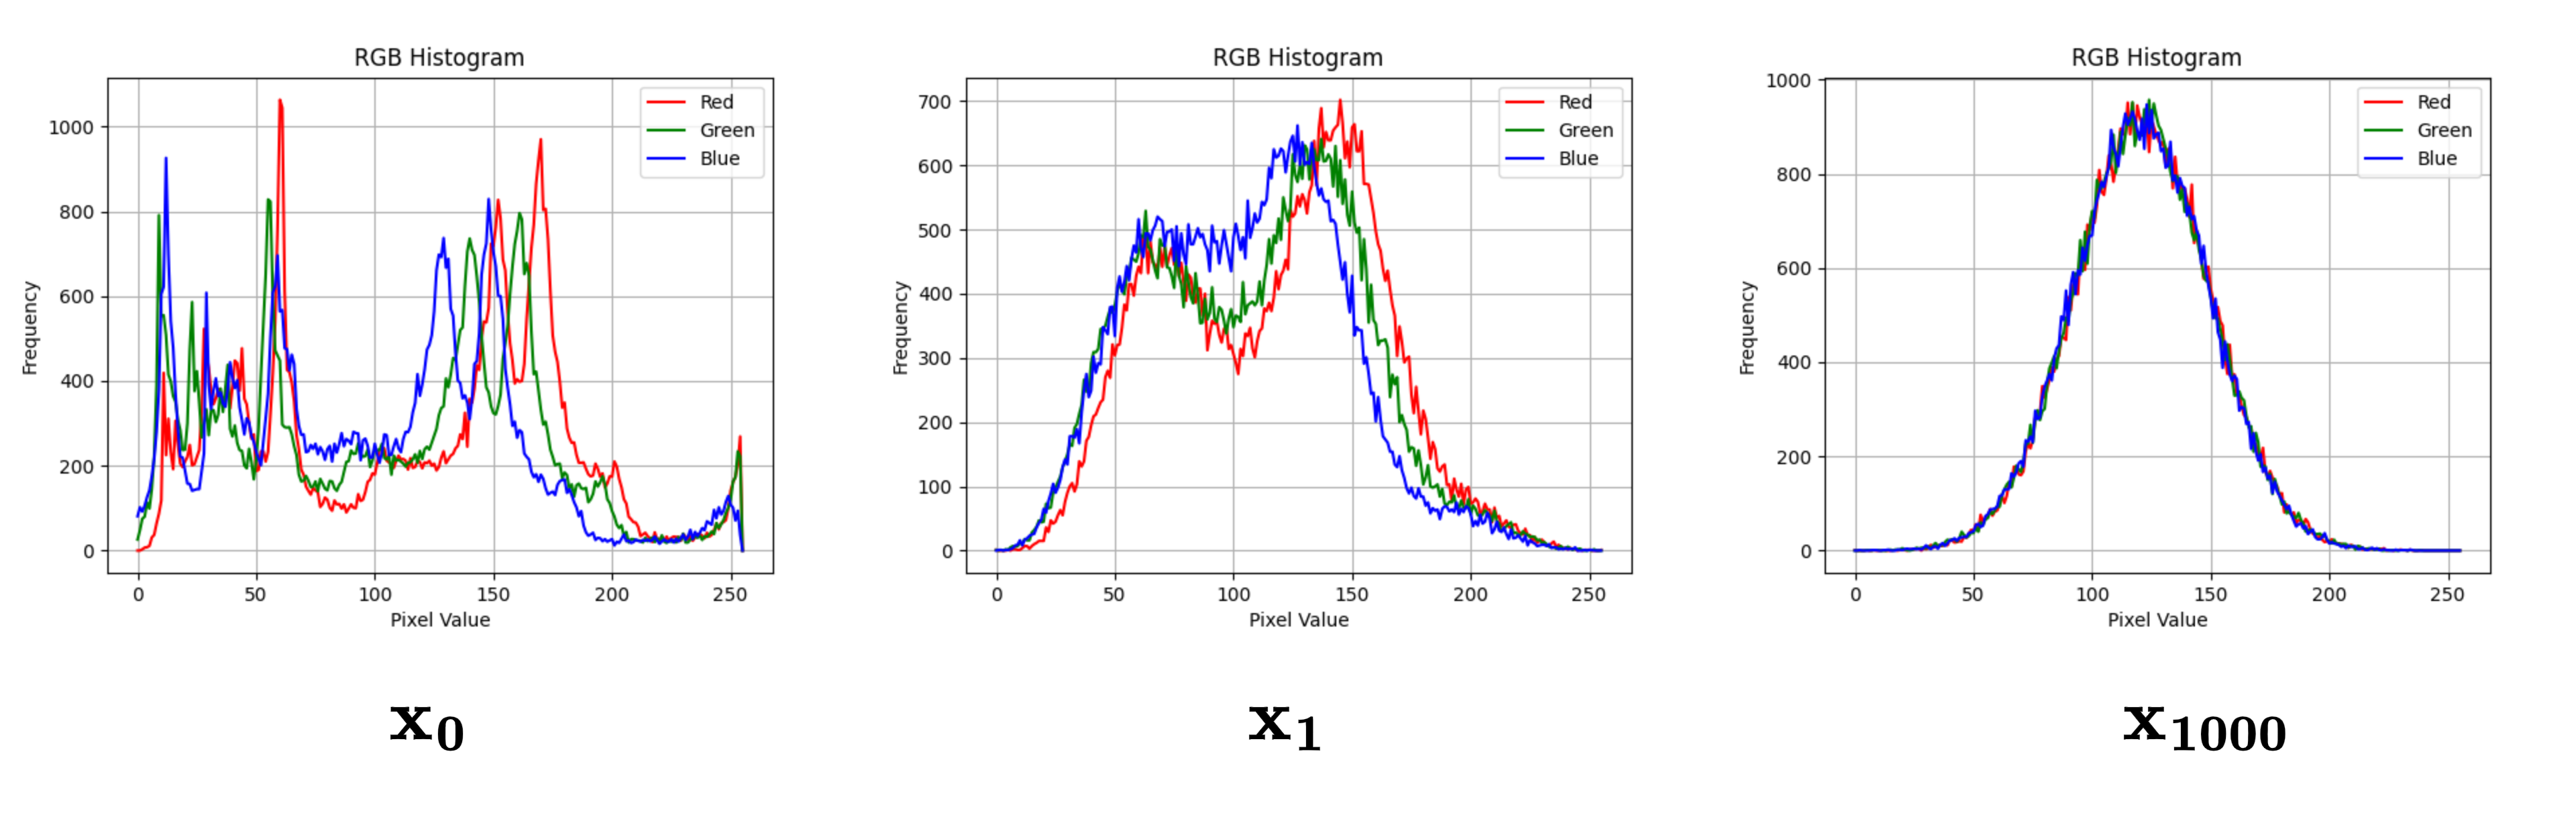
\includegraphics[width = \textwidth]{img/Histogram.png}
 \vspace{0.1cm}
 \caption{Histogram visualization for the forward process}
 \label{figure:Histogram}
\end{figure}

The ennoising process converted a data sample to a normal-distributed sample. Now we establish a process denoises a normal-distributed sample to a sample approximated to a data distribution. The reason is that we can minimize each sample during the ennoising and denoising processes to derive a suitable denoising process. Starting from the standard Gaussian noise $\overline{\xbf}_N\sim p_\theta(\overline{\xbf}_0):=\N(\mathbf{0},I_d)$, we need a decent way of performing denoising to retrieve $p_\text{data}$. Here we parameterize the reverse transitions by an U-Net \cite{ho2020denoising} as Gaussian distributions
\begin{equation}
 \label{equation:ddpm_reveverse}
 p_\theta(\overline{\xbf}_{n-1}|\overline{\xbf}_{n})=\N(\overline{\xbf}_n;\bm{\mu}(\overline{\xbf}_{n},i),\bm{\Sigma}(\overline{\xbf}_{n},i)), n=1,\ldots,N
\end{equation}
which constitutes the reverse joint probability density
\begin{equation}
 p_\theta(\overline{\xbf}_0,\ldots,\overline{\xbf}_N)=p_\theta(\overline{\xbf}_0)\prod\limits_{n=1}^Np_\theta(\Tilde{\xbf}_n|\overline{\xbf}_{n-1}).
\end{equation}
We would like to train the model so that we can generate samples via the reverse Markov processes, i.e. $p_\theta(\overline{\xbf}_0)\approx p_{\text{data}}(\xbf_0):=q(\xbf_0)$. An
apparent estimation of the parameter $\theta$ is that the forward and reverse states coincide correspondingly, i.e. $\xbf_n\approx\overline{\xbf}_{n}$, for $n=1,\ldots,N$ and $\xbf_N\approx\overline{\xbf}_{0}\sim\N(\mathbf{0},\mathbf{I}_d)$. As such, we should
expect the joint density with respect to the forward and the reverse processes are equal, i.e.
$$p_\theta(\overline{\xbf}_0,\ldots,\overline{\xbf}_N)\simeq q(\xbf_0,\ldots,\xbf_N).$$

Therefore, we can minimize the Kullback-Leibler divergence (see Equation \ref{definition:KL-divergence}) from $q(\xbf_0,\ldots,\xbf_N)$ to $p_\theta(\overline{\xbf}_0,\ldots,\overline{\xbf}_N)$.
\begin{equation}
 \label{equation:KL-yang}
 D_{\text{KL}}(q(\xbf_0,\ldots,\xbf_N)\| p_\theta(\overline{\xbf}_0,\ldots,\overline{\xbf}_N)) = \EE_{q(\xbf_0,\ldots,\xbf_N)}\left[\dfrac{q(\xbf_0,\ldots,\xbf_N)}{p_\theta(\overline{\xbf}_0,\ldots,\overline{\xbf}_N)}\right].
\end{equation}

\begin{figure}[H]
 \centering
 \scalebox{0.8}{
  \begin{tikzpicture}[->,>=stealth,shorten >=1pt,auto,node distance=2.3cm,semithick]
   % Forward process
   \node[state,minimum size=1.2cm] (A)  {$\xbf_0$};
   \node[state,minimum size=1.2cm,fill=lightgray] (B) [right of=A] {$\xbf_1$};
   \node[state,minimum size=1.2cm,fill=lightgray] (C) [right of=B] {$\xbf_2$};
   \node        (D) [right of=C] {$\cdots$};
   \node[state,minimum size=1.2cm,fill=lightgray] (E) [right of=D] {$\xbf_{N-2}$};
   \node[state,minimum size=1.2cm,fill=lightgray](F) [right of=E] {$\xbf_{N-1}$};
   \node[state,minimum size=1.2cm,fill=lightgray] (G) [right of=F] {$\xbf_N$};

   \path (A) edge              node {} (B)
   (B) edge              node {} (C)
   (C) edge              node {} (D)
   (D) edge              node {} (E)
   (E) edge              node {} (F)
   (F) edge              node {} (G);

   \node (image) [below of=D]{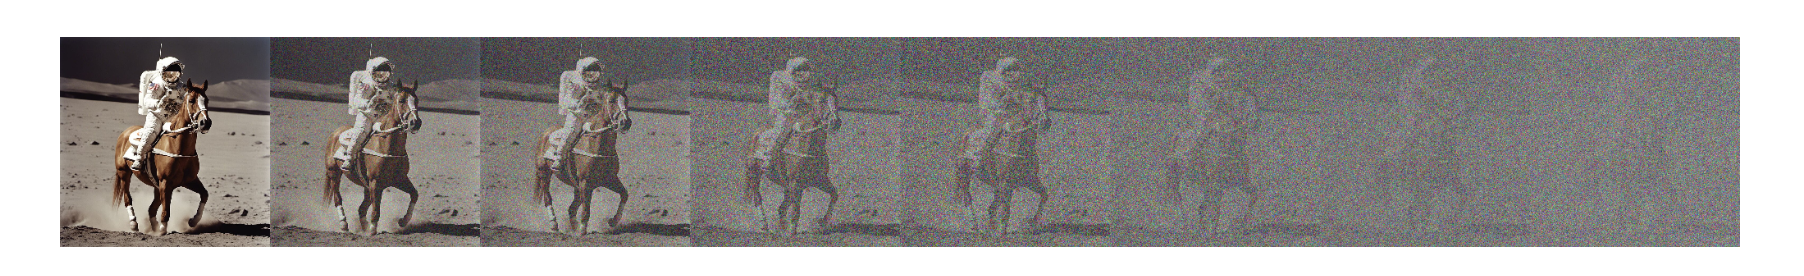
\includegraphics[width=\textwidth]{img/diffusion-illustration.png}};

   % Reverse process
   \node        (K) [below of=image] {$\cdots$};
   \node[state,minimum size=1.2cm,fill=lightgray] (J) [left of=K] {$\overline{\xbf}_{2}$};
   \node[state,minimum size=1.2cm,fill=lightgray] (I) [left of=J] {$\overline{\xbf}_{1}$};
   \node[state,minimum size=1.2cm] (H) [left of=I] {$\overline{\xbf}_N$};
   \node[state,minimum size=1.2cm,fill=lightgray] (L) [right of=K] {$\overline{\xbf}_{N-2}$};
   \node[state,minimum size=1.2cm,fill=lightgray] (M) [right of=L] {$\overline{\xbf}_{N-1}$};
   \node[state,minimum size=1.2cm,fill=lightgray](N) [right of=M] {$\overline{\xbf}_0$};

   \path (I) edge              node {} (H)
   (J) edge              node {} (I)
   (K) edge              node {} (J)
   (L) edge              node {} (K)
   (M) edge              node {} (L)
   (N) edge              node {} (M);
  \end{tikzpicture}
 }
 \caption[An illustration of DDPMs by Markov processes.]{An illustration of DDPMs by Markov processes. }
 \label{figure:diffusion-illustration}
\end{figure}

Now we will see how SDEs are applied, by using arbitrary intermediate time points. Let $\{\beta_t\}_{t\ge0}$ be the set of scheduled noise variance.
Let $\Delta t>0$ be an arbitrary time step. We follow Song et al. \cite{song2020score} to define $\beta(t)=\dfrac{\beta_t}{\Delta t_0}$ and thus
\begin{align*}
 \xbf_{t+\Delta t}-\xbf_{t}
  & = (\sqrt{1-\beta_t\Delta t}-1)\xbf_{t}+\sqrt{\beta_t}\sqrt{\Delta t}\bm{\epsilon}_{t}       \\
  & =(\sqrt{1-\beta_t\Delta t}-1)\xbf_{t}+\sqrt{\beta_t}(\mathbf{W}(t+\Delta t)-\mathbf{W}(t)).
\end{align*}

As $\Delta t\to 0$, we use an approximation
\begin{equation}
 \sqrt{1-\beta(t)\Delta t} - 1\approx -\dfrac{1}{2}\beta(t)\Delta t
\end{equation}
to arrive at a forward SDE
\begin{equation}
 \label{equation:song-sde}
 \d \xbf(t)=-\dfrac{1}{2}\beta(t)\xbf(t)\d t+\sqrt{\beta(t)}\d \mathbf{W}(t).
\end{equation}
Using Theorem \ref{theorem:reverse-time-sde}, the corresponding reverse-time SDE is
\begin{equation}
 \d \xbf_t = \left[-\dfrac{1}{2}\beta_t \xbf_t-\beta_t\nabla_{\xbf_t}\log p(\xbf_t, t)\right]\d t + \beta(t)\d \mathbf{W}_t.
\end{equation}
Therefore, using forward-backward SDEs, we only have to approximate $\nabla_{\xbf_t}\log p(\xbf_t, t)$, called the score function of $X_t$ i.e. to train a score network
$$\mathbf{s}_\theta(\xbf,t) \approx \nabla_{\xbf_t}\log p_t(\xbf_t)$$
instead of a network to approximate $\bm{\mu}(\overline{\xbf}_{n},i)$ and $\bm{\Sigma}(\overline{\xbf}_{n},i)$.

\subsection{Schrödinger Bridge}
Whereas unconditional diffusion models generate new samples in the dataset distribution, conditional diffusion models transform a sample from an initial distribution $p_{\A}$ to a target distribution $p_{\B}$. Schrödinger Bridge (SB) is an entropy-regularized optimal transport model that considers the following forward and backward SDEs \cite{schrodinger1932theorie}. In this discussion of SB, let us simplify the diffusion time interval to $[0,1]$. The forward-reverse SDEs in SB is given by
\begin{align}
 \label{equation:sb-fw}
 \d\xbf_t & = [\mathbf{f}_t + \beta_t\nabla\log\Psi(\xbf_t,t)]\d t + \sqrt{\beta_t}\d \mathbf{W}_t,           & \,\,\, \xbf_0\sim p_{\A}  \\
 \label{equation:sb-bw}
 \d\xbf_t & = [\mathbf{f}_t - \beta_t\nabla\log\hat{\Psi}(\xbf_t,t)]\d t-\sqrt{\beta_t}\d \bar{\mathbf{W}}_t, & \,\,\, \xbf_1\sim p_{\B}.
\end{align}

\begin{theorem}
 If $\Psi,\hat{\Psi}\in C^2(\RR^d,[0,1])$ satisfying
 \begin{equation}
  \label{equation:sb-condition}
  \begin{cases}
   \dfrac{\partial\Psi(\xbf,t)}{\partial t} = -\nabla \Psi^\top f-\dfrac{1}{2}\beta\Delta\Psi                      \\
   \dfrac{\partial\hat{\Psi}(\xbf,t)}{\partial t} = -\mathrm{div} (\hat{\Psi} f)+\dfrac{1}{2}\beta\Delta\hat{\Psi} \\
  \end{cases}
 \end{equation}
 The boundary conditions are $\Psi(x,0)\hat{\Psi}(x,0)=p(x,0)$ and $\Psi(x,1)\hat{\Psi}(x,1)=p(x,1)$.
 Then (\ref{equation:sb-bw}) is the reverse-time SDE of (\ref{equation:sb-fw}).
\end{theorem}
\begin{proof}
 The condition (\ref{equation:sb-condition}) suggests Nelson duality between $\Psi$ and $\hat{\Psi}$ \cite{nelson2020dynamical}
 $$\Psi(x,t)\hat{\Psi}(x,t)=p(x,t).$$
 Hence,
 $$\log\nabla\Psi(x,t) + \log\nabla\hat{\Psi}(x,t)=\log\nabla p(x,t).$$
 According to Theorem \ref{theorem:reverse-time-sde}, the reverse-time SDE of (\ref{equation:sb-fw}) is
 \begin{align*}
  \d X_t
   & = [f_t + \beta_t\nabla\log \Psi - \beta\nabla\log p(x,t)]\d t + \sqrt{\beta}\d W                             \\
   & = [\mathbf{f}_t - \beta_t\nabla\log\hat{\Psi}(\xbf_t,t)]\d t-\sqrt{\beta_t}\d \bar{\mathbf{W}}_t.
 \end{align*}
\end{proof}

\begin{theorem}
 Let (\ref{equation:sb-fw}) and (\ref{equation:sb-bw}) be a pair of forward-reverse SDEs. Then $\nabla\log\hat{\Psi}(x,t)$ and $\nabla\log{\Psi}(x,t)$ are the score functions of the following SDEs, respectively
 \begin{align}
  \label{equation:sde-psihat}
  \d X_t & = f_t\d t + \sqrt{\beta_t} \d W, & X_0\sim \nabla\log\hat{\Psi}(x,0) \\
  \label{equation:sde-psi}
  \d X_t & = f_t\d t + \sqrt{\beta_t} \d W, & X_0\sim \nabla\log{\Psi}(x,1).
 \end{align}
\end{theorem}
\begin{proof}
 Write the forward Kolmogorov equations and substitute conditions (\ref{equation:sb-condition}) to yield the results.
\end{proof}

\section{Vision Transformer}
\label{section:transformer}
Transformer \cite{vaswani2017attention} revolutionized the field with its innovative approach to sequential, contextual modeling, primarily to solve the next word prediction task. The model architecture consists of two fundamental components, namely Positional Embedding and Attention Mechanisms, which are also widely used in other models, especially our concerning related works. For instance, Vision Transformer (ViT) built upon this groundwork \cite{dosovitskiy2020image} marked a significant milestone by demonstrating that a pure Transformer could outperform CNNs in image feature extraction. SegFormer \cite{xie2021segformer}, one of the models applied in our watermark removal pipeline, improves ineffective settings in ViT for semantic segmentation task.

In this section, we discuss in details the building blocks of Transformer. Then we finally summarize the architecture dataflow. Firstly, let us denote by $\mathbf{X}=(\xbf_1,\ldots, \xbf_N)\in\RR^{D\times N}$ the sequence of tokens fed to the input of the neural network.

\subsection{Positional Embedding}
Recurrent Neural Networks \cite{rumelhart1986learning} was the first attempt to model sequential data, especially for sentences in NLP tasks. Positional Embedding serves as an alternative for deep learning architectures so that the dataflow is fully feedforward. The method modifies each token $\xbf_n, n\in\{1,\ldots,N\}$ element-wise to reflect positional information by

\begin{equation}
  \xbf_n^{(d)} \leftarrow \xbf_n^{(d)} + \mathrm{PE}(n,d),
\end{equation}
where $\mathrm{PE}(n,d)$ is a positional encoding function, for $n\in\{1,\ldots,N\}$ and $d\in\{1,\ldots,D\}$. In Transformer, the authors hypothesized that the effect of each pair of tokens to each other depends on the distance between them i.e. for each $m\in\{1,\ldots,N\}$, there exists a linear transformation $\bm{\Phi}^{(m)}$ such that

\begin{equation}
  \bm{\Phi}^{(m)}\xbf_n = \xbf_{n+m},
\end{equation}

where $n\in\NN$ satisfying $0\le n+m\le N$. Hence, given that $D$ is even, they decided to use the sinusoid for positional encoding

$$\mathrm{PE}(n,d) =
  \begin{cases}
    \sin(\omega_k\cdot n), \text{ if } d = 2k \\
    \cos(\omega_k\cdot n), \text{ if } d = 2k+1,
  \end{cases}$$
where $\omega_k = \dfrac{1}{10000^{2k/D}}$.

Indeed, the function seamlessly meets their requirement. Consider two tokens $\xbf_n$ and $\xbf_{n+m}$, each at two dimensions $2k$ and $2k+1$. We aim to find a matrix $M^{(m)}_k=\begin{pmatrix}u_1 & u_2 \\ v_1 & v_2\end{pmatrix}\in\RR^{2\times2}$ such that
\begin{equation}
  \label{equation:sinusoid-transformation}
  M\begin{pmatrix}
    \sin(\omega_k\cdot n) \\
    \cos(\omega_k\cdot n)
  \end{pmatrix} = \begin{pmatrix}
    \sin(\omega_k\cdot (n+m)) \\
    \cos(\omega_k\cdot (n+m))
  \end{pmatrix}.
\end{equation}

Since
\begin{align*}
  \sin(\omega_k\cdot (n+m)) & = \sin(\omega_k\cdot n)\cos(\omega_k\cdot m) + \cos(\omega_k\cdot n)\sin(\omega_k\cdot m)  \\
  \cos(\omega_k\cdot (n+m)) & = \cos(\omega_k\cdot n)\cos(\omega_k\cdot m) - \sin(\omega_k\cdot n)\sin(\omega_k\cdot m).
\end{align*}

Plug the expansion into Equation \ref{equation:sinusoid-transformation}, we get the solution
\begin{equation}
  M^{(m)}_k =
  \begin{pmatrix}
    \cos(\omega_k\cdot m)  & \sin(\omega_k\cdot m)  \\
    -\sin(\omega_k\cdot m) & \sin(\omega_k\cdot m),
  \end{pmatrix}
\end{equation}
which only depends on $m$. Therefore, we have
\begin{equation}
  \begin{pmatrix}
    M^{(m)}_1 & 0      & \cdots & 0             \\
    0         & \ddots & \cdots & 0             \\
    0         & \cdots & 0      & M^{(m)}_{D/2}
  \end{pmatrix} \xbf_n = \xbf_{n+m}.
\end{equation}

\begin{figure}[ht]
  \centering
  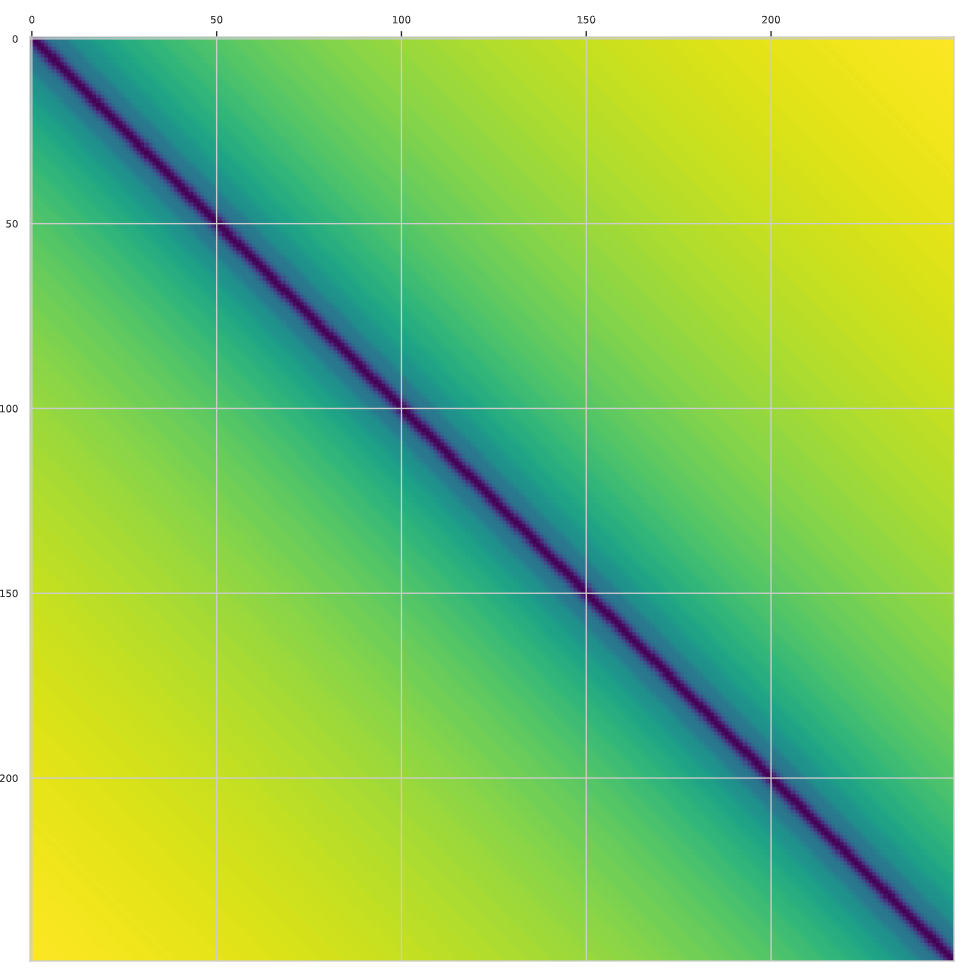
\includegraphics[width=0.6\textwidth]{img/positional-embedding-heatmap.png}
  \captionsetup{justification=centering} % Center the caption
  \caption[Positional embedding heatmap]{Positional embedding heatmap. Source \href{harrisonpim.com/blog/understanding-positional-embeddings-in-transformer-models}{Harrison Pim's blog}.}
  \label{figure:positional-embedding-heatmap}
\end{figure}

The effect of sinusoid positional embedding is illustrated in Figure \ref{figure:positional-embedding-heatmap}. We compute the dot product of every pair of token whose positions from $0$ to $250$. A darker color indicates a higher value of dot product. We can see a pattern that the heatmap gets brighter when going away from the diagonal, meaning that closer tokens are higher relevant.

\subsection{Attention Mechanisms}

Attention mechanisms are motivated by human volitional and nonvolitional cues \cite{zhang2023dive}. Let say while you are thirsty, there are three objects in front of you, a glass of orange juice, a politics newspaper and a deep learning book. Nonvolitionally, you pay attention to the orange juice. After you quenched, as a deep learning enthusiast, you deliberately take the deep learning book instead of the politics newspaper, which is an instance of volitional cues. Parameterized fully-connected layers or even non-parameterized layers like max or average pooling can be regarded as to bias selection over sensory inputs. The set of three given objects is called a \textit{context}. A nonvolitional state is called a \textit{key}. We may not capture all features of the context, for example, how the newspaper smells, but only a few sensory inputs depending on your nonvolitional state current mental and physical state, like the thirst in the example.  A sensory feature is called a \textit{value}, paired with a key. Attention mechanisms also model volitional cues, like your enthusiasm in deep learning, which in the language of attention mechanisms, is called a \textit{query}.

\begin{figure}[ht]
  \centering
  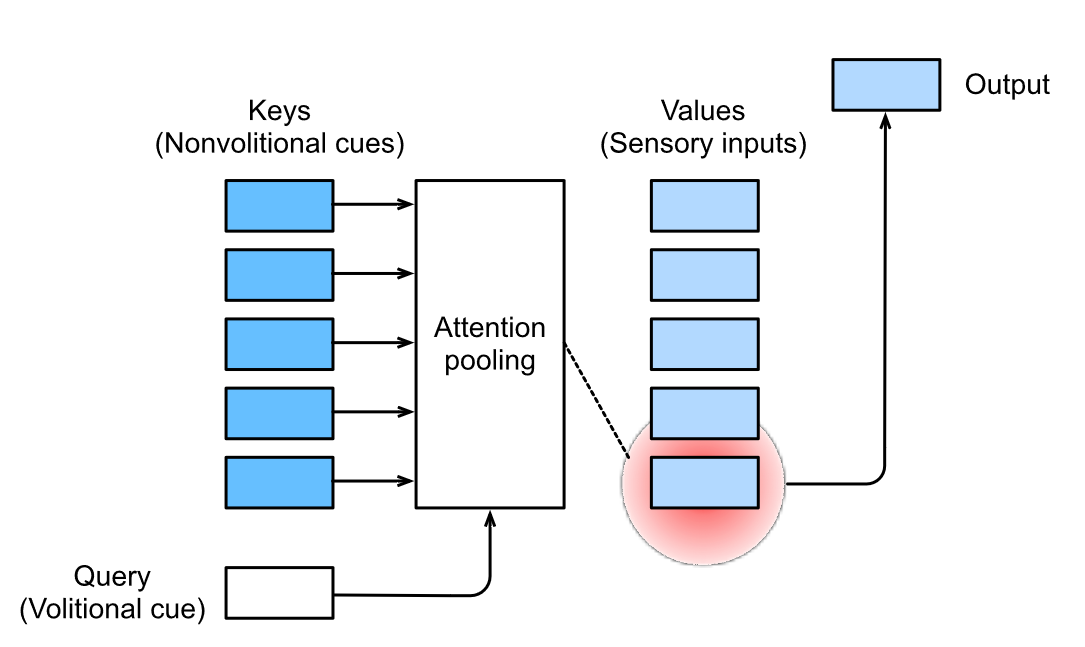
\includegraphics[width=0.75\linewidth]{img/attention.png}
  \vspace{0.25cm}
  \caption[Overview of Attention Mechanism]{Overview of Attention Mechanism \cite{zhang2023dive}}
  \label{figure:attention}
\end{figure}

Mathematically, a context includes a set of tokens after positional embedding, say $\mathbf{Y}=(\ybf_1,\ldots, \ybf_N)\in\RR^{D\times N}$. The tokens correspond to the values $\mathbf{V}=(\v_1,\ldots, \v_N)\in\RR^{D\times N}$, in result of the keys $\mathbf{K}=(\k_1,\ldots, \k_N)\in\RR^{d_k\times N}$. We also asset each token a query $\q_n, n\in\{1,\ldots,N\}$ and denote $\mathrm{Q} = (\q_1,\ldots, \q_N)$. A query effects more considerably on a token $\ybf_n, n\in\{1,\ldots,N\}$, if it highly matches the corresponding key $\k_n$. We model the matching score by dot product. For this reason, the queries are selected to have the same dimension as the keys. For each query $\q_n, n\in\{1,\ldots,N\}$, the authors computed the matching scores $\q_n \mathbf{K}^\top$, then normalized into $\mathrm{softmax}\left(\dfrac{\q_n\mathbf{K}^\top}{\sqrt{d}}\right)$.
More compactly,
\begin{equation}
  \mathrm{Attention}(\mathbf{Q}, \mathbf{K}, \mathbf{V}) = \mathrm{softmax}\left(\dfrac{\mathbf{Q}\mathbf{K}^\top}{\sqrt{d}}\right)\mathbf{V}.
\end{equation}
The authors used three learnable matrices $\mathbf{W_v}\in \RR^{D\times D}$, $\mathbf{W_k}\in \RR^{d_k\times D}$ and  $\mathbf{W_q}\in \RR^{d_k\times D}$ to extract the values, keys and queries from the tokens i.e.
$$\mathbf{V} = \mathbf{W_v}\mathbf{Y}, \mathbf{K} = \mathbf{W_k}\mathbf{Y} \text{ and } \mathbf{Q} = \mathbf{W_q}\mathbf{Y}.$$

In practice, the authors employed \textit{Multi-head Attention}. In instead of one value matrix, $h:=\dfrac{D}{d_v}$ value matrices $\mathbf{W_v}\in \RR^{D\times d_v}$ are used, where $d_v$ divides $D$, yielding $h$ $d_v$-dimensional output tokens in parallel. The outputs are then concatenated to $D$-dimensional tokens. In general, the keys and queries can be generated from two different sequence, which we called Cross Attention.

\subsection{Transformer Architecture}
\begin{figure}[ht]
  \centering
  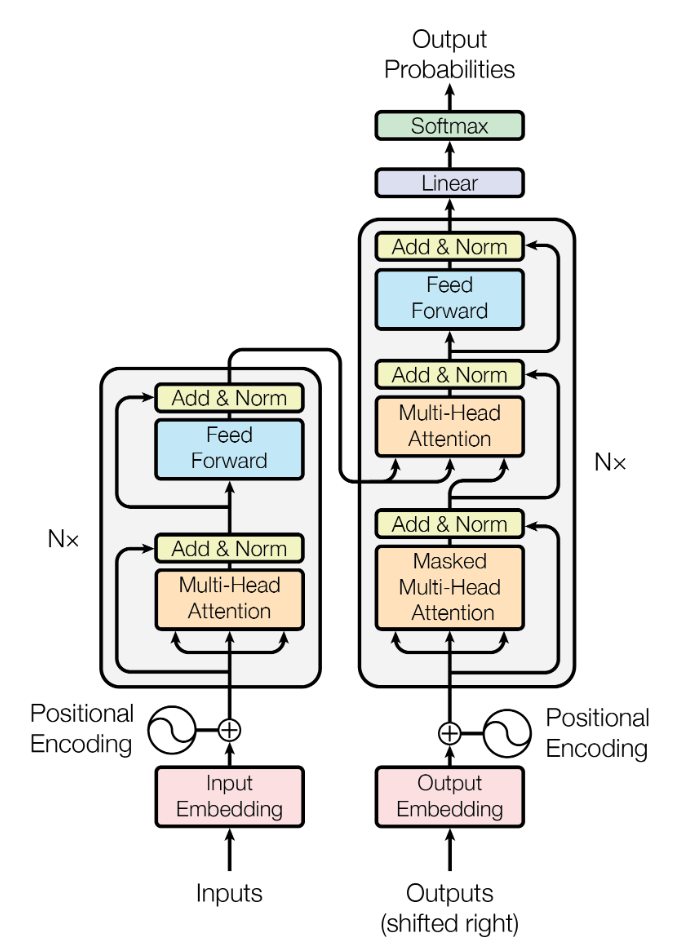
\includegraphics[width=0.5\linewidth]{img/transfomer.png}
  \vspace{0.5cm}
  \caption[Transformer architecture]{Transformer architecture \cite{vaswani2017attention}}
  \label{figure:transformer-architecture}
\end{figure}

As illustrated in Figure \ref{figure:transformer-architecture}, the Transformer follows an encoder-decoder structure \cite{cho2014learning}. The encoder consists of $N$ blocks, each built up by a multi-head attention layer followed by a feedforward layer. The decoder takes the sequence of right-shifted tokens $(\xbf_2,\ldots, \xbf_{N+1})$, masks and processes multi-head attention for themselves, before feeding to other $N$ identical blocks as the encoder, together with the output of the encoder. Final output is a probability distribution for the next token over the dictionary.

The token $\ybf_n, n\in\{1,\ldots,N\}$ is then modified by a linear combination of the values, weighted by the normalized matching scores
$$\ybf_n \leftarrow \ybf_n + \mathrm{softmax}\left(\dfrac{\q_n\mathbf{K}^\top}{\sqrt{d}}\right)V.$$

\subsection{Vision Transformer}
The Transformer architecture is not limited to NLP tasks. Vision Transformer (ViT) is the first work to show that this architecture outperforms traditional Convolutional Neural Networks (CNNs) on image classification tasks \cite{dosovitskiy2020image}. Figure \ref{figure:ViT} illustrated the design of ViT, where each image is divided into patches and treated as a sequence of token which is almost similar to original Transformer.

\begin{figure}
    \centering
    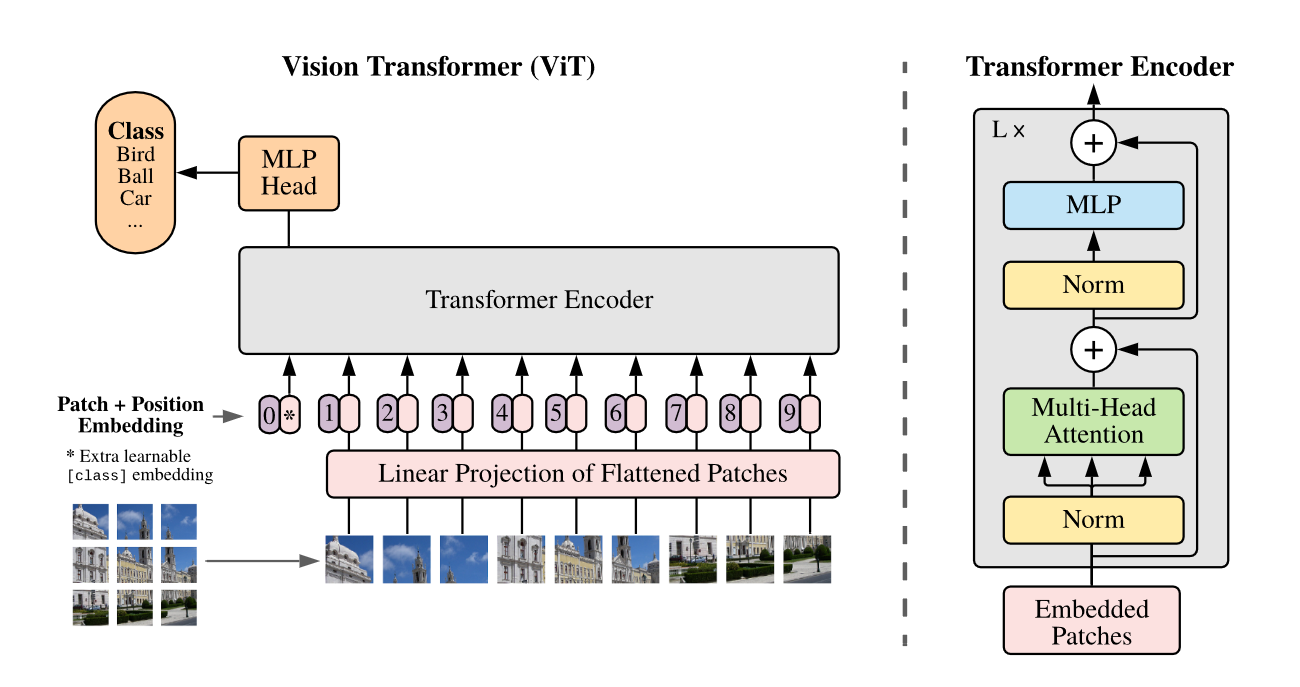
\includegraphics[width=0.8\linewidth]{img/ViT.png}
    \caption[Vision Transformer architecture]{Vision Transformer architecture \cite{dosovitskiy2020image}}
    \label{figure:ViT}
\end{figure}



% \subsection{An Application in Computer Vision}

% \begin{figure}[ht]
%   \centering
%   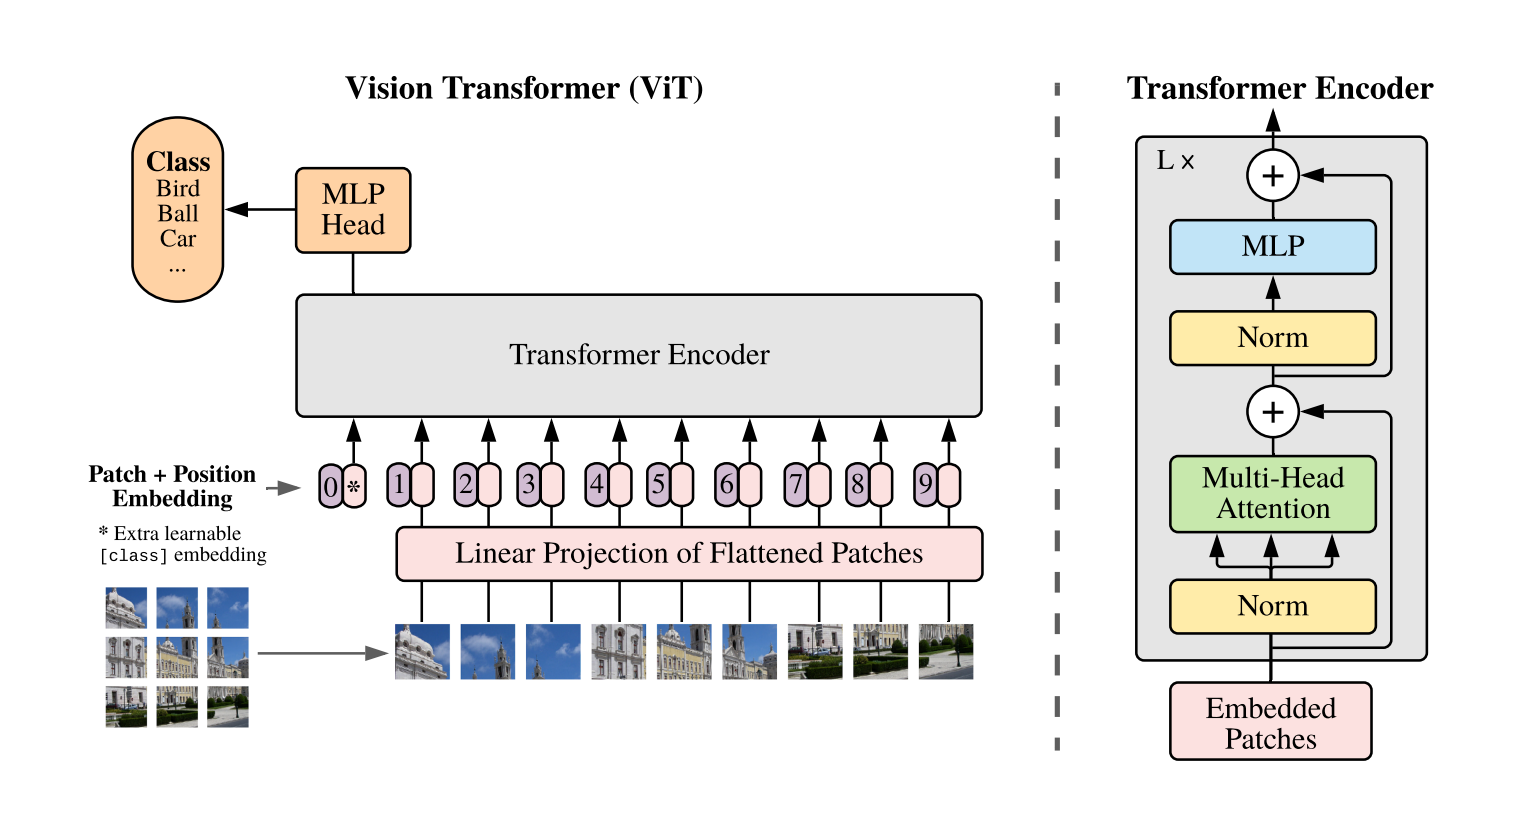
\includegraphics[width=0.75\linewidth]{img/vision-transformer.png}
%   \caption{Vision Transformer Architecture}
%   \label{figure:vision-transformer-architecture}
% \end{figure}

% Note that the number of parameters Attention Mechanism does not depend on the context size $N$. According to the specific problem and dataset, multilayer perceptrons are added for the final output. For generative models, given a sequence of symbols, the expected output is a categorical distribution of symbols in the corpus, to predict the next symbol.



% \section{Image Segmentation}

% Image segmentation and types
Image segmentation is a well-known problem in Computer Vision, where an image is divided into several parts (segments) to serve a purpose.

There are other types of segmentation. In our scope, we opted for semantic segmentation models for our watermark detection task in our watermark removal pipeline. For example, in Figure \ref{figure:sam-all}, Segment Anything model \cite{kirillov2023segment} return segmented pixels belonging to available classes.

We selected semantic segmentation instead of detection, because the segmented result fits the object, rather than returns a bounding box.

\begin{figure}[ht]
    \centering
    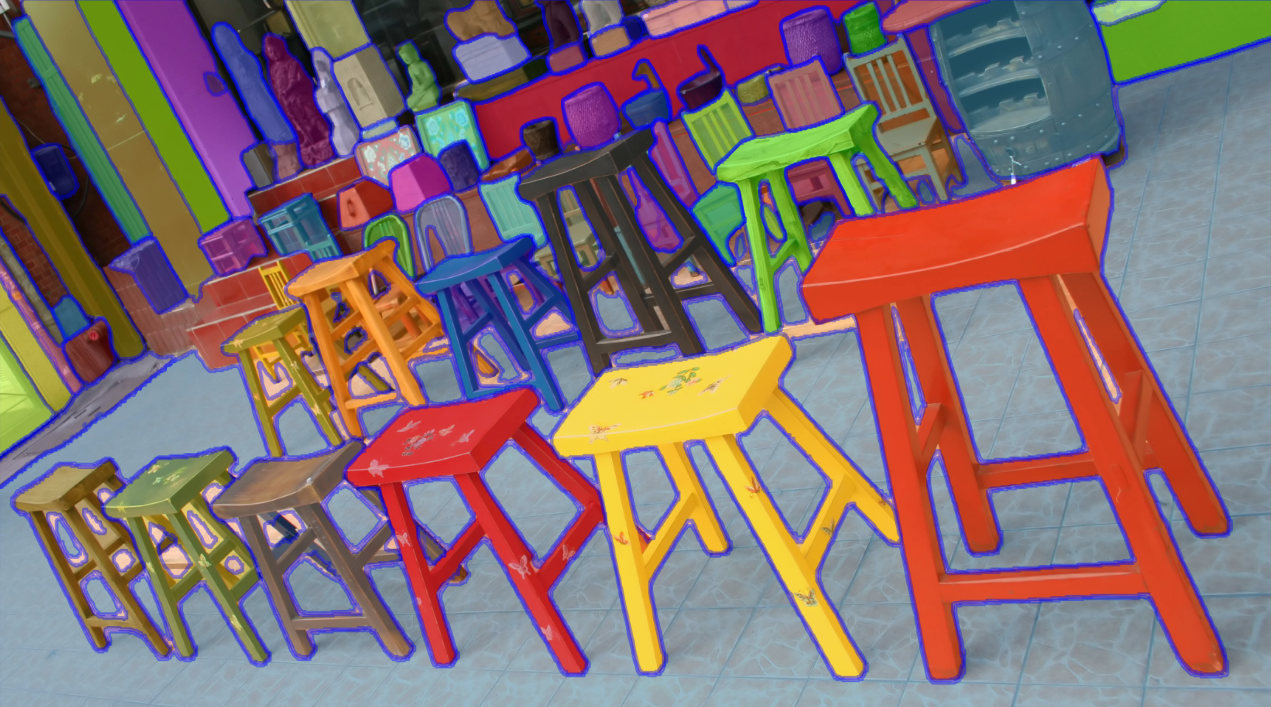
\includegraphics[width=0.8\textwidth]{img/sam-segmented-all.png}
    % 
    \caption[An image segments returned by SAM]{An image segments returned by SAM \cite{kirillov2023segment}}
    \label{figure:sam-all}
\end{figure}

% Why chosen
% In our proposed pipeline, we firstly segment an image to predict the region occupied by the watermark. Especially, Semantic segmentation suffices for our needs as it simply entails predicting which pixels are probable components of a watermark, but no further specific instances. 

% If using detection, we have to train another model to detect watermarks of a given training set, and hope that the model can generalize to unseen watermarks. Meanwhile, the watermark in an image will automatically be segmented out as it does not belong to any available class.


% There are commonly three types of segmentation. Regional segmentation divides an image into several constituent regions, usually based on the correlation between pixels in the image. Semantic segmentation classifies each pixel to one of aforementioned classes, or assigns to each pixel a distribution on the classes. This second type of segmentation is a generalization of classification. Instance segmentation goes beyond semantic segmentation, that it also detects difference instances of the same class in an image.






\chapter{Related Works}
\label{chapter:related-works}
\thispagestyle{empty}
\section{Watermark Overview}
Watermarking involves modifying a piece of content to include a message related to that content. The origins of watermarking can be traced back to medieval times, evolving alongside advancements in papermaking and the growing need for document authentication and security. The practice first emerged in 13th century Italy, where papermakers integrated basic designs or symbols into paper molds, resulting in subtle variations in thickness. When held up to light, these watermarks became visible, functioning as identification for the papermaker or as an indicator of quality. Watermarking involves modifying a piece of content to include a message related to that content. The origins of watermarking can be traced back to medieval times, evolving alongside advancements in papermaking and the growing need for document authentication and security. The practice first emerged in 13th century Italy, where papermakers integrated basic designs or symbols into paper molds, resulting in subtle variations in thickness. When held up to light, these watermarks became visible, functioning as identification for the papermaker or as an indicator of quality.

By the 18th century, watermarks began incorporating more elaborate designs and patterns, often reflecting the brand of the paper manufacturer or adding an artistic touch. This period marked a shift from purely utilitarian watermarks to those with aesthetic appeal. In the early 20th century, the advent of digital technology led to the transformation of traditional paper watermarks into digital counterparts. In the realm of digital media, these digital watermarks serve diverse purposes, including safeguarding copyright, authenticating content, and facilitating tracking. They are imperceptible to the human eye and became prevalent in the late 20th century, embedded within digital files such as images or documents. Nowadays, watermarks continue to fulfill essential roles in security, branding, and authentication across physical and digital domains, adapting to the evolving needs of industries and technologies.

Paper watermarks first appeared in Italy in 1282, over a thousand year since papermaking had been invented in China. The marks were made by adding thin wire patterns to the paper molds. The earliest watermarks were used for practical functions such as identifying the molds on which sheets of papers were made, or as trademarks for ownership, or they might just represent mystical signs or serve as decoration. By the eighteenth century, they have been used in Europe and America for precise purposes, trademarks and manufacturing records. It was also the first time watermarks were used as anticounterfeiting measures on money and other documents. From that time, watermark embedding systems and watermark attacking systems prompted advances for each other, as a subbranch of security and steganography.

\subsection{Watermark Embedding}
In general, watermarks can be as simple as an extra logotype or text added to an image that are subtle with human visual system, or an imperceptible signal embedded to an original signal. Subsequently, watermarks can be broadly classified into two primary categories - visible and invisible.

Visible watermarks are intentionally noticeable and easily seen by the human eye. Typically overlaid onto the surface of an image or document, they often consist of logos, text, or symbols. The principal aim of visible watermarks is to identify the origin or ownership of the content and deter unauthorized use. While effective in conveying ownership, visible watermarks may occasionally impact the aesthetic appeal of the content.

On the other hand, invisible watermarks are like secret codes you cannot see right away. They get mixed into the picture using digital tricks, such as adding noise or embedding unique code within the pixels of a digital image without changing how it looks. Invisible watermarks do different jobs, like protecting copyrights, proving if something is real, or keeping track of things. They are useful for digital stuff, like pictures or documents, because you do not see any changes on the outside. To find invisible watermarks, you need special computer programs or smart processes that can uncover the hidden information.

In our project, we are focusing on those watermarks that catch your eye—the visible ones. They mess with the image when they are added, and that is the puzzle we are tackling. We are figuring out how to use a diffusion-based method to bring back the original image after we have wiped out those noticeable watermarks, like totally removing them from the picture.

We now then work on putting the watermark into images. The aim is to enhance the image's privacy, adding an extra layer of security. The introduction of a watermark provides a level of protection for the image. Watermarks come in various types, such as those made of text or images. In our project, we are specifically concentrating on image watermarks. Our objective is to embed the image watermark into the original image, making it challenging to identify or detect compared to text watermarks, which are somewhat easier to recognize. Subsequently, we plan to examine and remove these watermarks through detection methods.

There are various methods to incorporate a watermark into an image. Tao et al. \cite{tao2014robust} have researched some methods to embed a robust watermark, ranging from random embedding to intentional placement. In intentional embedding, the watermark can alter the image's appearance, making it challenging for humans to observe or confusing for classifier models, leading to incorrect predictions. In our approach, we choose to randomly embed the watermark within the image, in which details will be discussed in Chapter \ref{chap:experiment}. This section will delve into the specifics of our method for watermark embedding.


In general, watermarks can be as simple as an extra logotype or text added to an image that are subtle with human visual system, or an imperceptible signal embedded to an original signal. Those in the former case are conventionally called visible watermarks, where diffusion models can be applied to transform a watermarked region or the whole image into a realistic unwatermarked version. Those in the latter case are called invisible watermarks with two broad groups of generating models - \textit{communication-based} models and \textit{geometric models} \cite{cox2007digital}. We focus on visible watermarks only. A visible watermark embedding algorithm should satisfy some requirements, such as

\begin{enumerate}
    \item The watermark is perceptible in both gray and colored images.
    \item The watermark should be perceptible in pixels with different characteristics: texture, plain and edge.
    \item The watermark should not be too obtrusive.
    \item The watermark should be robust against several common attacks.
    \item Watermark embedding process should be automatic for kinds of images.
\end{enumerate}

An image can be represented a three-channel two-dimensional array. Compressed into the gray scale, each pixel takes integer values in the interval $[0,256]$.  The following watermark embedding model for binary watermark \cite{yu2013new} is based on the observation that the ability of human eyes to distinguish between two close pixel values tend to be highest in the interval $[64,128]$, i.e. for a pixel $p\in [64,128]$, a human may be able to distinguish between $p$ and $p+1$. Denote by $y$ this minimal perceptible difference. They approximate the relation as
\begin{equation}
    y=\begin{cases}
        -\dfrac{1}{8}p+6,             & \text{ if } p\in [0, 32]   \\
        -\dfrac{1}{32}p+3,            & \text{ if } p\in [33, 64]  \\
        -\dfrac{1}{96}p+\dfrac{1}{3}, & \text{ if } p\in [65, 255] \\
    \end{cases}
\end{equation}

\begin{figure}
    \centering
    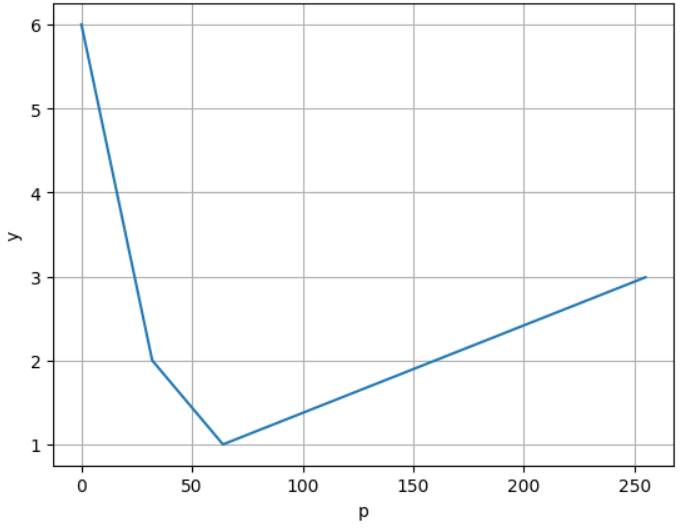
\includegraphics[width=0.5\linewidth]{img/resolution.png}
    \vspace{0.5cm}
    \caption{The approximation of human eye resolution on the gray scale}
    \label{figure:human-eye-resolution}
\end{figure}

Therefore, the difference between a clean pixel and a watermarked pixel must obey this human distinguishing ability. The watermark strength $\alpha$ depending on the pixel value is given by
\begin{equation}
    \alpha(p)=cy(p),
\end{equation}
where $c$ is a constant hyperparameter. The watermarked image is obtained pixel-by-pixel by
\begin{equation}
    p'(i,j)=p(i,j)+\alpha
    (p(i,j))w(i,j),
\end{equation}
where
\begin{itemize}
    \item $p(i,j)$ is the original pixel
    \item $w(i,j)\in\{0,1\}$ is the watermark value
\end{itemize}

The embedding process is applied for each channel and finally combined to a single watermarked image.

\subsection{Watermark Removal}
% intro with surveys
Digital watermarks are frequently employed for copyright identification in images, preventing unauthorized use of online images. Additionally, techniques for attacking watermarks aim to effectively eliminate watermarks from host images. The strength of a watermark against such attacks is crucial for safeguarding image copyrights. Methods for removing watermarks have been investigated to assess and enhance the durability of watermarks. In this section, we will explore existing methods and discuss our approach to watermark removal.

Oldest methods for getting rid of watermarks usually require users to point out where the watermark is located, and then they use special features to remove it, such as Independent Component Analysis \cite{pei2006novel} or Color Space Transformation \cite{park2012identigram}. Also, some methods make use of multiple images \cite{dekel2017effectiveness} \cite{gandelsman2019double}. But, these methods need a lot of information ahead of time, and they only work well on a limited number of examples.

\begin{figure}[H]
    \centering
    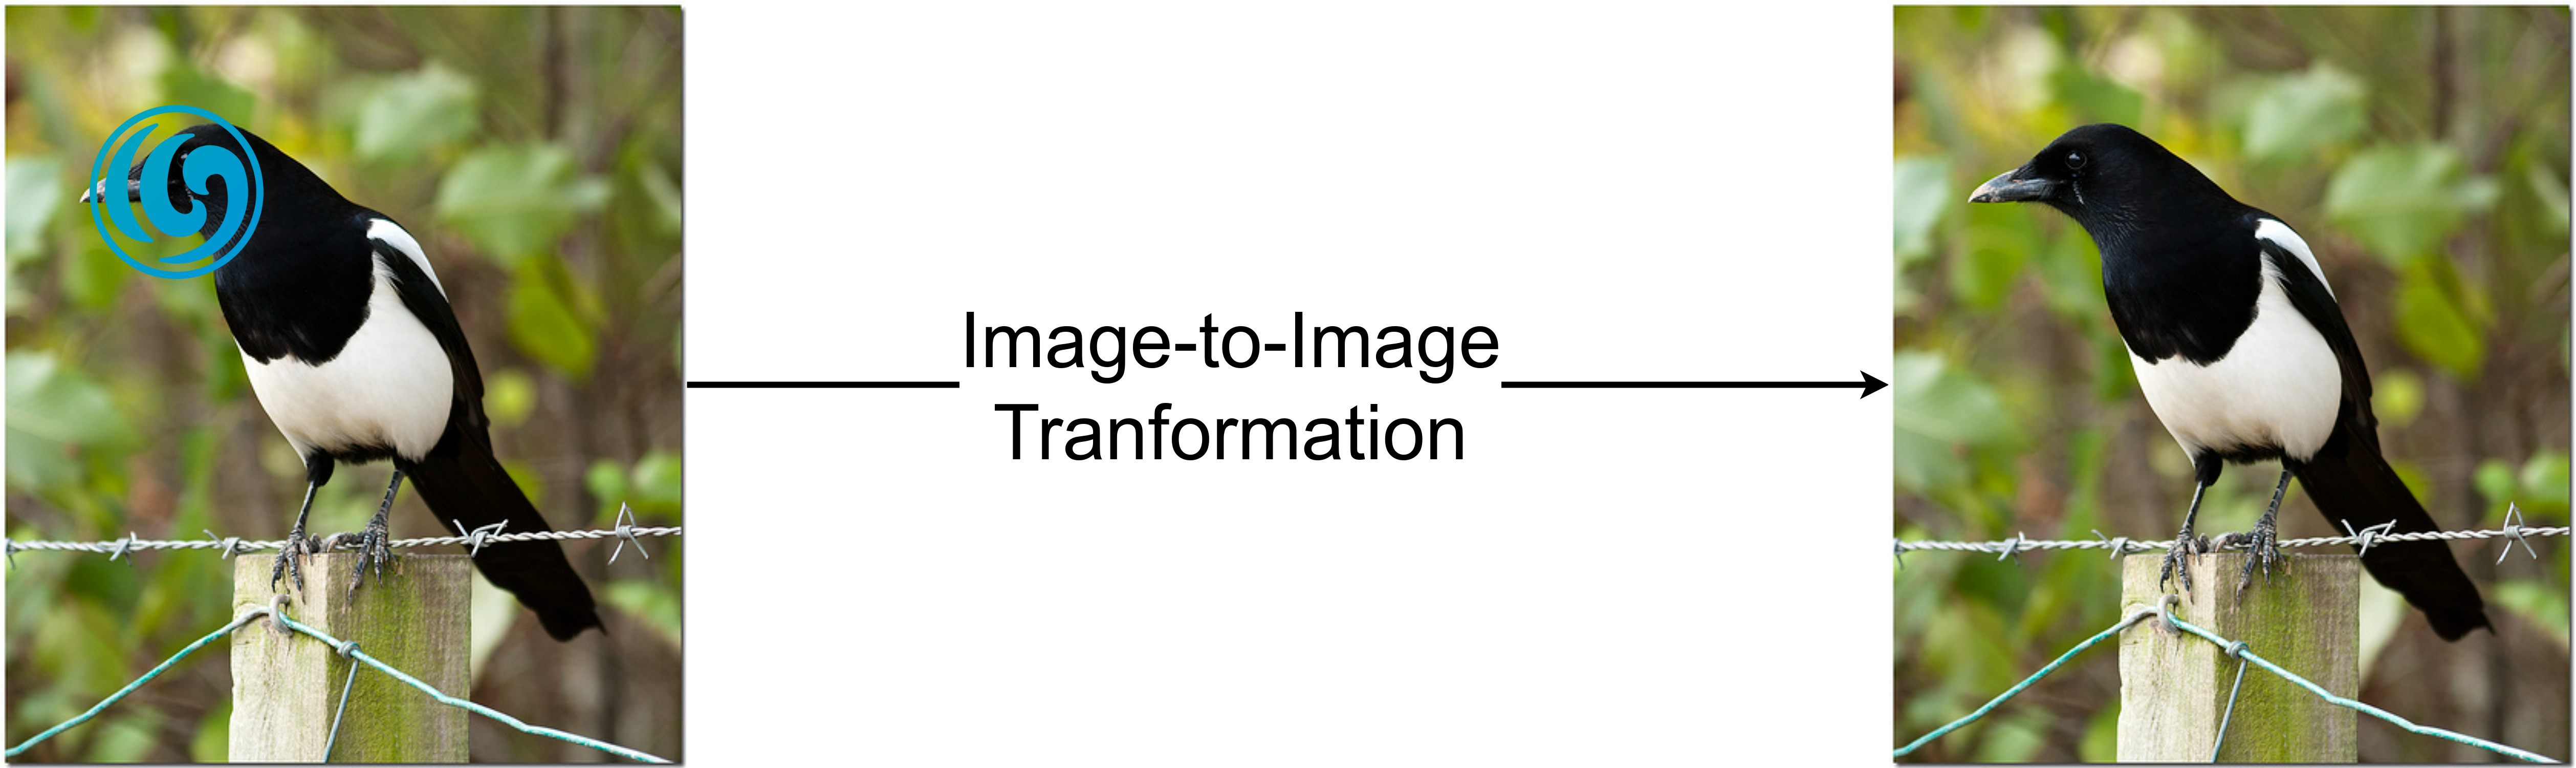
\includegraphics[width=0.75\linewidth]{img/watermark_removal_1.png}
    \caption{Watermark Removal with Image-to-Image methods}
    \label{figure:img2img1}
\end{figure}

More recently, deep learning-based methods show great power in many computer vision tasks \cite{he2016deep}, and this approach has been applied to remove visible watermarks too \cite{li2019towards} \cite{cheng2018large}  \cite{hertz2019blind}. But, before using these methods, you need a detection model that can already identify watermarks \cite{cheng2018large}, or they only focus on getting rid of the watermark without thinking about the whole image as an Image-to-Image Translation problem \cite{li2019towards}, as generally illustrated in Figure \ref{figure:img2img1}. Plus, the datasets they often use only have gray-scale watermarks. Nowadays, though, most watermarks are in color. Recently, a method was designed to find, erase, and fix the motif in just one go \cite{hertz2019blind}. However, these methods do not pay much attention to learning about the damaged part of the image.

% \textcolor{red}{CNN version (U-Net): https://arxiv.org/pdf/2403.05807.pdf}
% \textcolor{red}{Note about one-stage watermark removal}
% \subsection{Image-to-Image methods}
% Summary some methods in Image-to-Image


\section{Two-stage Watermark Removal}

The mentioned methods in the previous section mainly focus on transforming a watermarked image to an unwatermarked one, which we can think of as one-stage watermark removal. In this section, we discuss models relevant to our approach, including segmentation models (SegFormer and SAM) and a diffusion-based inpainting model (I$^2$SB). These models build up our two-stage watermark removal pipeline, which is discussed in details in Chapter \ref{chap:experiment}.

Before Transformer (see Section \ref{section:transformer}), U-Net \cite{ronneberger2015u} was popular for semantic segmentation task. Segmentation Transformer (SETR) \cite{zheng2021rethinking} was one of early applications of Transformer for semantic segmentation, achieving considerable improvement over CNNs. SegFormer \cite{xie2021segformer} was developed in motivation of this work, with Efficient Self-attention. Recently, Segment Anything Model (SAM) \cite{kirillov2023segment} was designed for the ability to run on low-end devices. In this section, we discuss two latest models, SegFormer and SAM, which are also those used in our watermark segmentation phase.

\subsection{SegFormer}
\label{intro:segformer}
SegFormer made use of multi-head attention mechanism, but highly specialized for semantic segmentation task.

\begin{figure}[ht]
  \centering
  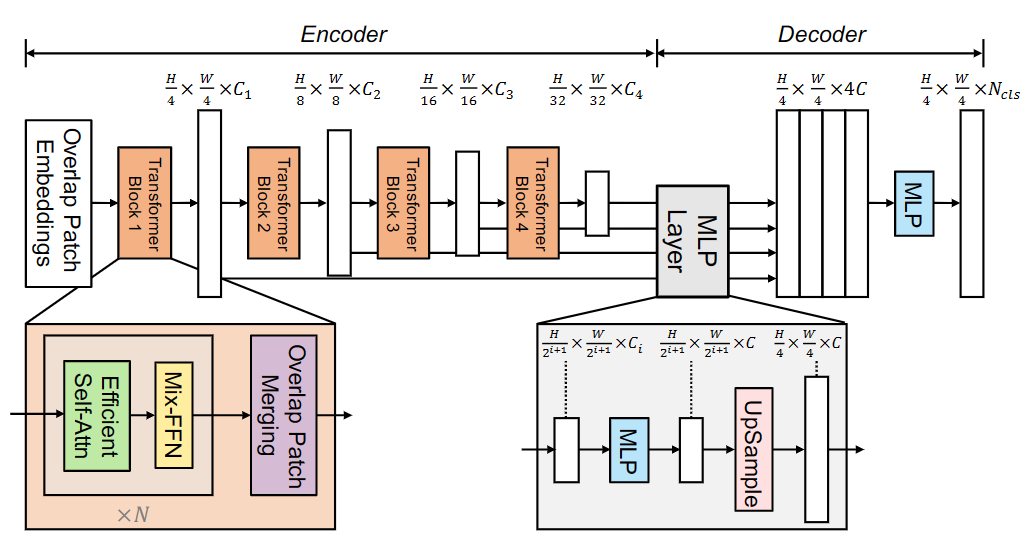
\includegraphics[width=0.7\linewidth]{img/segformer.png}
  \vspace{0.5cm}
  \caption{SegFormer Architecture}
  \label{figure:segFormer-architecture}
\end{figure}

As can be seen in Figure \ref{figure:segFormer-architecture}, there are two major components in the architecture, namely the Overlap Patch Embedding, Transformer Block and the MLP Layer, whose details are delved into in following sections.

\subsubsection{Encoder}

\textbf{Overlap Patch Embedding.} Originally in Vision Transformer (ViT) \cite{dosovitskiy2020image}, an image of size $H\times W\times 3$ is divided into $\frac{HW}{P^2}$ patches of size $P\times P \times 3$. Each patch is then flattened and linearly projected in to a $C$-dimensional vector, where $C>3$, returning a sequence of size $\frac{HW}{P^2}\times C$. The patches in this case have no overlaps.

SegFormer employed Overlap Patch Embedding, with two additional hyperparameters $s$ and $p$ for stride and padding, similarly to CNNs. In particular, the authors of SegFormer used $(P,s,p)\in\{(7,4,3), (3,2,1)\}$, result in a sequence size $\frac{HW}{4} \times C$, while preserved the local continuity around those patches.

\textbf{Efficient Self-Attention.} This is an subblock of the Transformer block. After extracted as the keys $\mathbf{K}$ and queries $\mathbf{Q}$ of the same size as the sequence, the matrices go through a self-reduction process of ratio $r$. For instance, let $N=\frac{HW}{4}$, we have
\begin{align*}
  \mathbf{K'} & = \mathrm{Reshape}\left(\dfrac{N}{r}, C\cdot r\right)(\mathbf{K}) \\
  \mathbf{K}  & = \mathrm{Linear}\left(\dfrac{N}{r}, C\right)(\mathbf{K'}).
\end{align*}
Thus, $\mathbf{K}$ is reduced to dimension $\frac{N}{r}\times C$ and similarly for $\mathbf{Q}$. The complexity is reduced from $O(N^2)$ to $O\left(\frac{N^2}{r}\right)$ comparing to original Multi-head Attention \cite{xie2021segformer}. In particular, the matrices $\mathbf{K}$, $\mathbf{Q}$ and $\mathbf{V}$ are constrained to be of equal size, enabling them to be generated simultaneously from the token sequence, which results in improved computational performance.

\textbf{Mix-FFN.} This subblock is used as an alternative to Positional Encoding in ViT that only takes care of the distance between the tokens. The approach in ViT leads to the drop of accuracy for semantic segmentation task when the test set resolution differs from the training set. In SegFormer, the authors included a convolutional layer to encode positional information
$$\xbf_{\mathrm{out}} = \mathrm{MLP}(\mathrm{GELU}(\mathrm{Conv_{3\times 3}(\mathrm{MLP}(\xbf_{in}))})).$$
Their approach was based on an argument that adding PE to feature map is not necessary in semantic segmentation, and was empirically proved to be sufficient for this task.


\textbf{Overlapped Patch Merging.} This is the final subblock of the Transformer block that reshapes the previous output to size $\frac{W}{2}\times \frac{H}{2} \times C$, and processes similarly to Overlap Patch Embedding, returning a sequence of size $\frac{WR}{16}\times C_1$, where $C_1>C$. The other three following Transformer Blocks work similar, getting the sequence after the previous block and outputting a sequence of size $\frac{WR}{2^{2i+2}}\times C_i$, for $i\in\{2,3,4\}$.

\subsubsection{Decoder}
After each Transformer Block, the sequence is reshaped to get hierarchical representation of size $\frac{W}{2^{i+1}}\times \frac{H}{2^{i+1}}\times C_i$, for $i\in{1,2,3,4}$. Each representation goes through an MLP and then is unsampled to size $\frac{W}{4}\times \frac{H}{4}\times 3$. The representations are concatenated to $\frac{W}{4}\times \frac{H}{4}\times 12$. The last MLP (the blue block in Figure \ref{figure:segFormer-architecture}) gives the output $\frac{W}{4}\times \frac{H}{4}\times N_{\mathrm{cls}}$, where $N_{\mathrm{cls}}$ is the number of classes. Intersection over Union (mIoU) was selected to be the loss function.

\subsection{Segment Anything}
\label{sec:intro-sam}
The other choice for the watermark detection stage in our pipeline is the Segment Anything model (SAM) developed by Meta \cite{kirillov2023segment}, a considerable revolution in semantic segmentation task, as it allows prompts from user. The design is claimed to be optimized to work in real-time. The model consists of an image encoder, a prompt encoder and a lightweight mask decoder. We will delve into the details as follows.

\begin{figure}
  \centering
  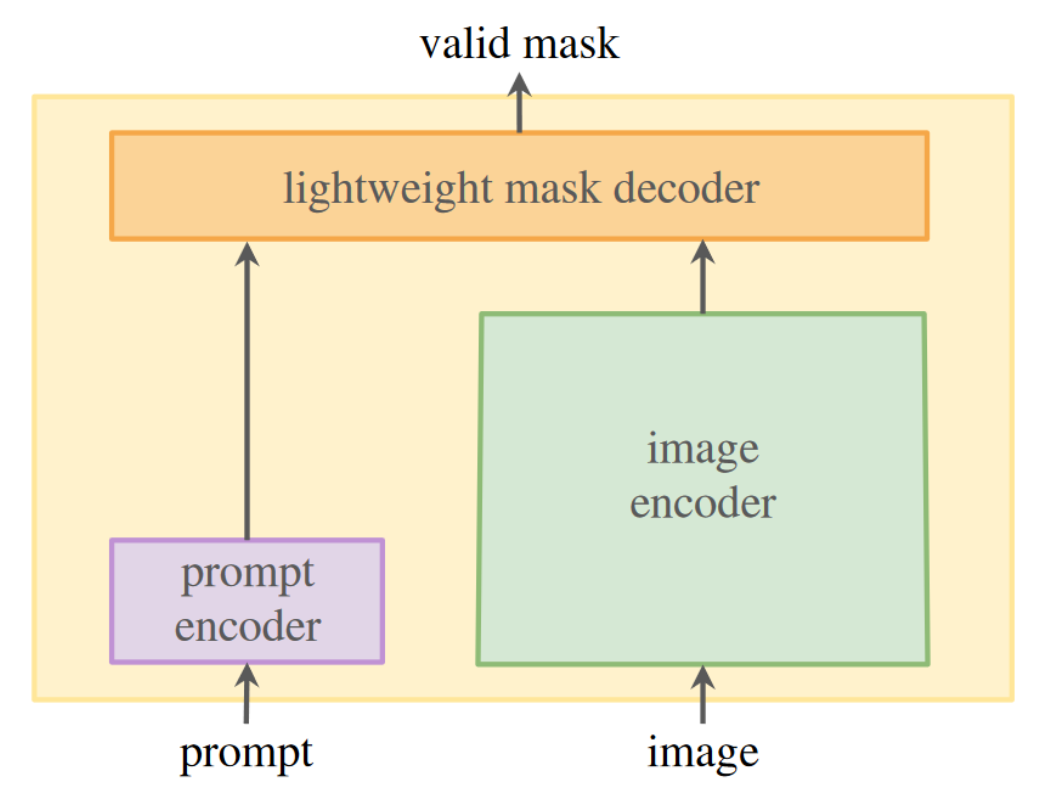
\includegraphics[width=0.6\textwidth]{img/segment-anything-model.png}
  \vspace{0.25cm}
  \caption[The overall architecture of Segment Anything model]{The overall architecture of Segment Anything model \cite{kirillov2023segment}}
\end{figure}

\subsubsection{Image Encoder}
The authors of the Segment Anything model followed standard practices, that they firstly rescale an image and pad the shorter side to attain an input resolution of $1024\times1024$. They employed several ViT backbones \cite{dosovitskiy2020image}, one of them is a ViT-H/16, followed by a Masked Autoencoder \cite{he2022masked}, returning an image of 16-time lower resolution. The image is then passed through convolutional layers to arrive at an output size of $256\times 64\times 64$.

\subsubsection{Prompt Encoder}
The model allows prompts of two types: sparse (points, boxes, text) and dense (masks). Each prompt is mapped to a $256$-dimensional vectorial embedding. A point is represented by the sum of a foreground-background learned embedding and a positional encoding. The latter value is a general approach of the sinusoid function called Fourier features \cite{tancik2020fourier}. A box is represented by an representation pair. For the top-left corner, the representation is the sum its positional encoding and its learned ``top-left corner'' embedding. A similar structure is applied for the bottom-right corner, except for that a learned ``bottom-right corner'' embedder is used. A text encoder can be any available one. The authors used continuous bag of words and Text Transformer \cite{vaswani2017attention} for their experiments. A mask is firstly converted a 4-time lower resolution than the input image. Then it is downscaled  by additional 4 times, using two $\mathrm{Conv}_{2\times 2}$ with stride 2 and output channels 4 and 16, respectively. A final $\mathrm{Conv}_{1\times 1}$ maps the channel dimension to $256$. Each layer is separated by GELU activations and layer normalization. Finally, the mask are added to the image element-wise. If there is no mask prompt, a learned embedding representing ``no mask'' is added to each image embedding location.

\subsubsection{Lightweight Mask Decoder}
The previous image embedding is treated as a set of $64^2$ 256-dimensional vectors. The lightweight mask decoder is designed using Cross Attention (see Section \ref{section:transformer}), as illustrated in Figure \ref{figure:segment-anything-model-mask-decoder}.

\begin{figure}[ht]
  \centering
  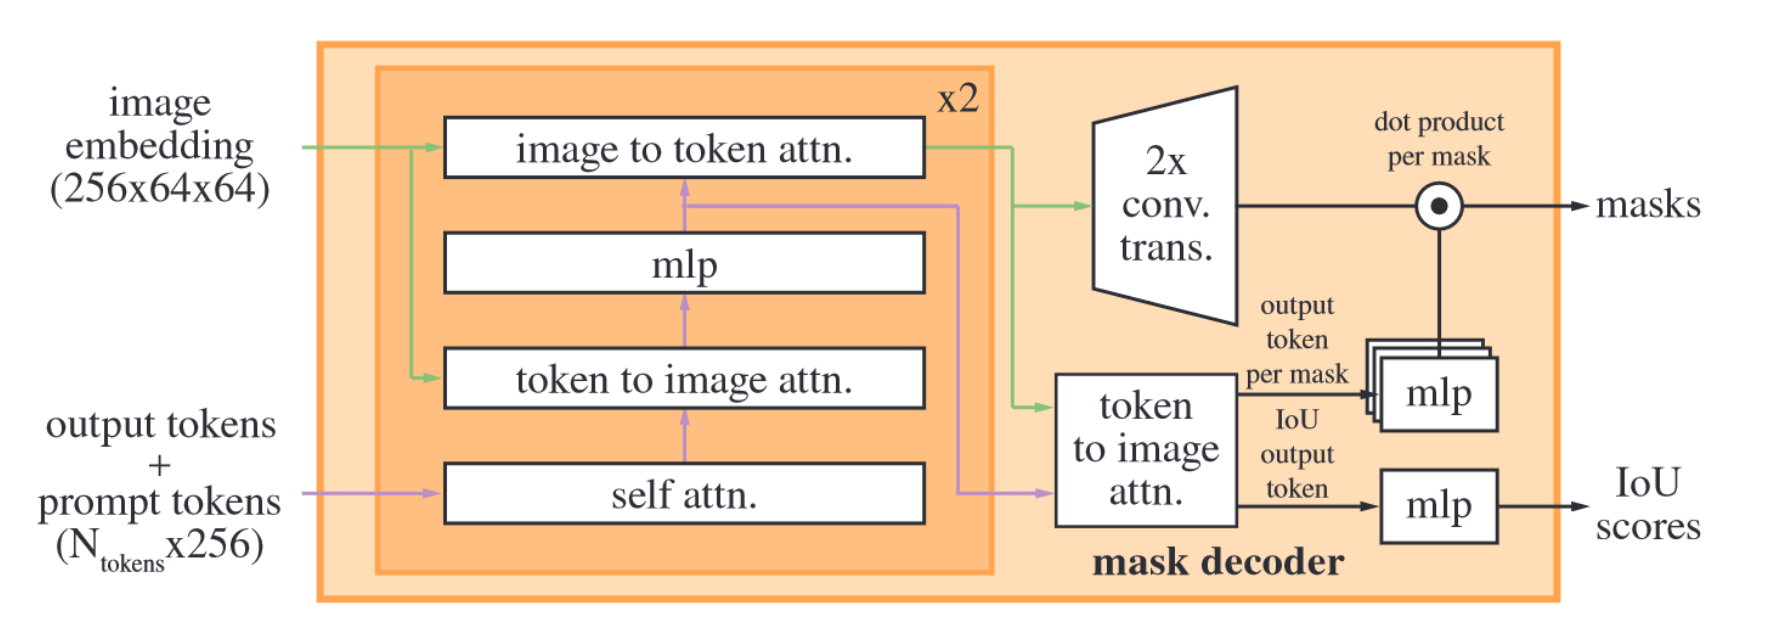
\includegraphics[width=0.6\textwidth]{img/segment-anything-model-mask-decoder.png}
  \vspace{0.25cm}
  \caption[The lightweight mask decoder design]{The lightweight mask decoder design \cite{kirillov2023segment}}
  \label{figure:segment-anything-model-mask-decoder}
\end{figure}

\begin{figure}[H]
  \centering
  \begin{subfigure}[b]{0.48\textwidth}
    \centering
    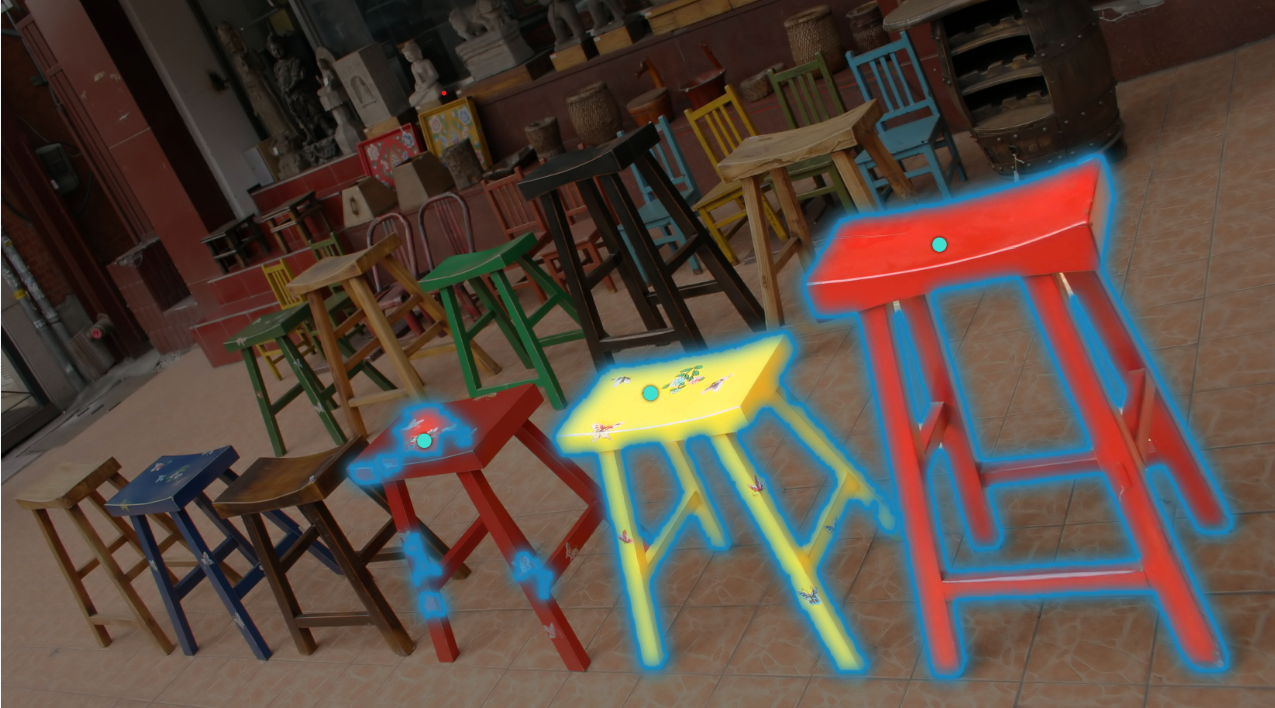
\includegraphics[width=\textwidth]{img/sam-segmented-after-point.png}
    \label{fig:sam_point}
  \end{subfigure}
  \hfill
  \begin{subfigure}[b]{0.48\textwidth}
    \centering
    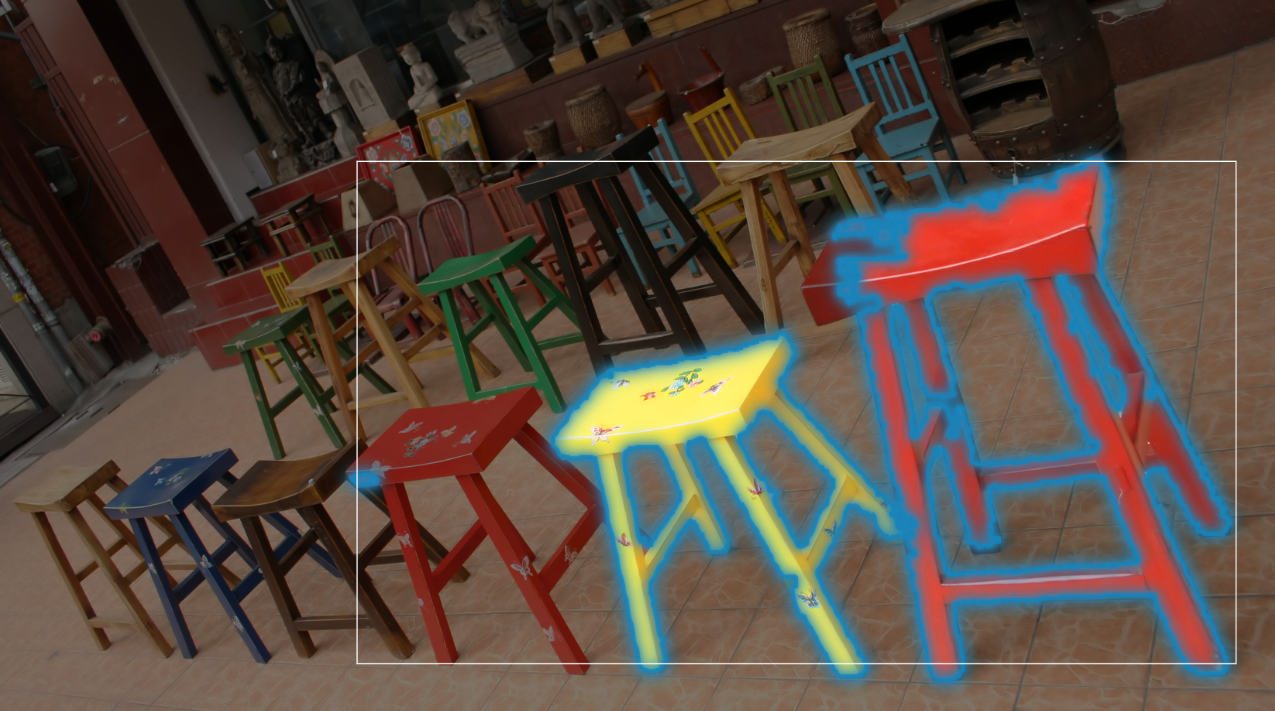
\includegraphics[width=\textwidth]{img/sam-segment-bounding-box.png}
    \label{fig:sam_box}
  \end{subfigure}
  \caption[Segmented regions returned by SAM]{Segmented regions returned by SAM. In the left figure, three points are selected, while in the right figure, a box is drawn. In both cases, the leftmost chair is not fully recognized.}
  \label{fig:sam_segments}
\end{figure}

\subsection{Image-to-Image Schrödinger Bridge}
\label{sec:i2sb}
Image inpainting is the process of restoring or completing portions of an image, the second phase in our watermark removal pipeline. After identifying the specific watermark location, image inpainting techniques can also be used to remove the visible watermarks \cite{huang2004attacking}. Thus, attention-guided inpainting methods, such as Partial Convolution \cite{liu2018image}, Contextual Attention \cite{yu2018generative} and Gated Convolution \cite{Yu:2018uw} are applicable to this task. Recently, Generative Adversarial Networks (GAN) \cite{goodfellow2014generative} and Image-to-Image Schrödinger Bridge (I$^2$SB) \cite{liu2023i2sb} are developed as state-of-the-art works. GAN trains two adversarial networks. A generator $G$ generates a sample $X$ as close to the dataset as possible and a discriminator $D$ labels the probability that $X$ is generated by $G$, not from the real dataset. Through adversarial training, $G$ and $D$ converge to the Nash equilibrium. On the other hand, I$^2$SB is developed recently from conditional diffusion models, using a tractable class of Schrödinger Bridge. As diffusion models are shown to beat GAN on image generation tasks \cite{dhariwal2021diffusion}, we present I$^2$SB as the main approach to our image inpainting task.

\begin{figure}[t]
  \begin{center}
    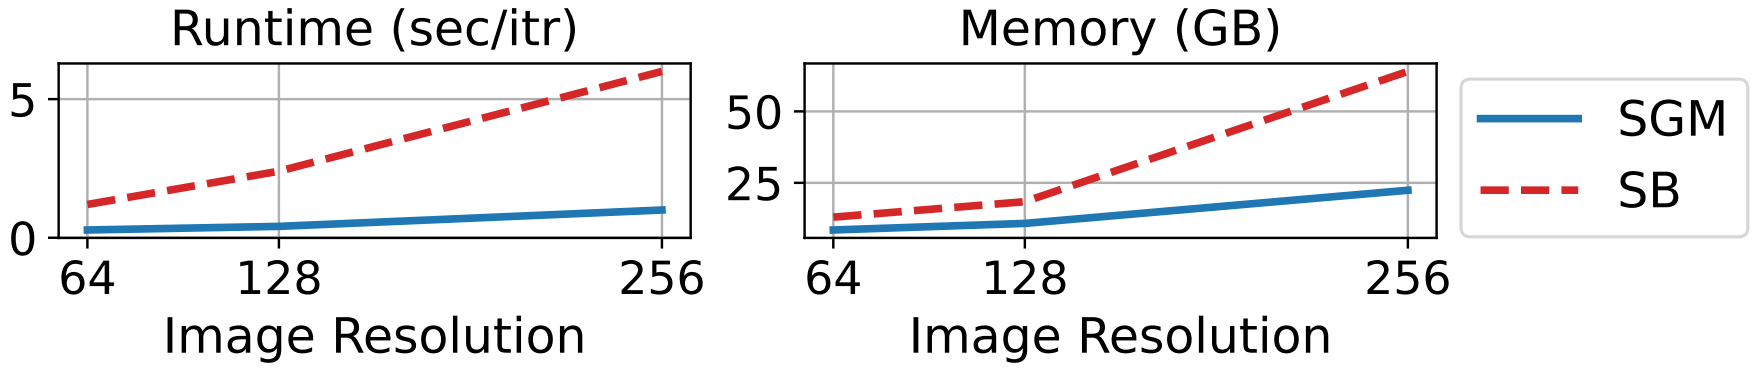
\includegraphics[width=0.85\columnwidth]{img/complexity.png}
    \caption[Complexity of SGM and SB]{
      Complexity of SGM and SB \cite{chen2021likelihood} On 256$\times$256 resolution, SB is 6$\times$ slower and consumes 3$\times$ memory.
    }
    \label{figure:complexity}
  \end{center}
\end{figure}

\begin{figure}[t]
    \centering
    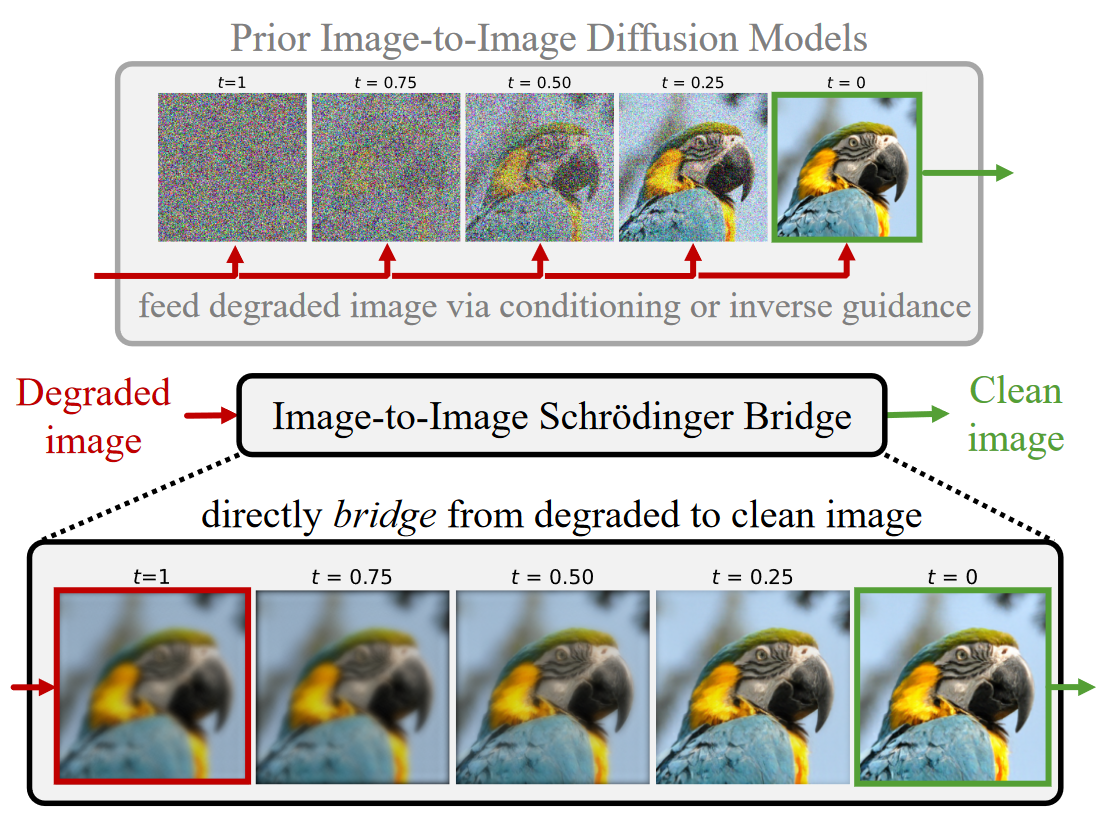
\includegraphics[width=0.6\linewidth]{diffusion-vs-sb.png}
    \caption{Difference between predominant non-conditional diffusion models and I$^2$SB}
    \label{figure:diffusion-vs-sb}
\end{figure}

Figure \ref{figure:complexity} illustrates the complexity of Likelihood Training of Schrödinger Bridge \cite{chen2021likelihood}, a previous SB approach (see Section \ref{section:diffusion-models}) for image generation. I$^2$SB employs a tractable class of SB for better training efficiency, cognizing that the train dataset is Dirac Delta distributed. The difference between non-conditional diffusion models and I$^2$SB can be seen in Figure \ref{figure:diffusion-vs-sb}. Non-conditional models generates a new sample in the image dataset distribution from the Gaussian noise, while I$^2$SB convert an image in the degraded distribution to an image in the clear distribution. 

\begin{sbtheorem}[Tractable SB with the Dirac Delta Boundary]
  \label{theo-dirac}
  Let $p(\cdot,0) := \delta_a(\cdot)$ be the Dirac delta distribution centered at $a\in\RR^d$. Then, the initial distributions in (\ref{equation:sde-psihat}) and (\ref{equation:sde-psi}) are given by
  \begin{equation}
    \label{equation:sb-dirac}
    \hat{\Psi}(\cdot,0)= \delta_A(\cdot), \Psi(\cdot,1)=\dfrac{p(\cdot, 1)}{\hat{\Psi}(\cdot,1)}.
  \end{equation}
\end{sbtheorem}

The Dirac delta assumption also implicitly appears in the denoising objective, which first computes the target $\nabla\log p(\xbf_t,t|\xbf_0=a)$ for each data point $a$, as the score between $\delta_{a}(\cdot)$ and Gaussian, then averages over $\xbf_0 {\sim} p_\A$. In this vein, Theorem \ref{theo-dirac} adopts the same boundary $\delta_{a}(\cdot)$ on one side and generalizes the other side from Gaussian to arbitrary $p_\B$. Based on the details provided in Table \ref{table:comp_diff}, it becomes evident that employing Theorem \ref{theo-dirac} enables us to transform the Schrödinger Bridge (SB) model, which is challenging to handle at $\nabla\log\hat{\psi}$ and demands substantial time and resources for training. With our model I$^2$SB, utilizing the degraded dataset allows us to generate a pair of information from the clean image. Consequently, the term $\nabla\log\hat{\psi}$ becomes manageable, enabling us to calculate the score with reduced resource requirements.


\begin{table}[H]
  \caption[Comparison of different diffusion models in boundary distributions and tractability]{
    Comparison of different diffusion models in boundary distributions and tractability of forward and backward drifts. Note that I$^2$SB requires paired information compared to standard SB}
  \label{table:comp_diff}
  \label{table:comp}
  \vskip 0.05in
  \begin{center}
    \begin{small}
      \begin{tabular}{rclcc}
        \toprule
        \textbf{Model} & \textbf{$\mathbf{p(\xbf_0)}$} & \textbf{$\mathbf{p(\xbf_1)}$} & \textbf{$\mathbf{\gradlog \Psi}$} & \textbf{$\mathbf{\gradlog \Psihat}$} \\ [0.5ex]
        \midrule
        (C)SGM
                       & $p_\A$                        & $\N(0,I)$                     & 0                                 & tractable                            \\[0.5ex]
        \textbf{I$^2$SB}
                       & $p_\A$                        & $p_\B(\cdot|\xbf_0)$          & intractable                       & tractable                            \\[0.5ex]
        SB
                       & $p_\A$                        & $p_\B(\cdot)$                 & intractable                       & intractable                          \\
        \bottomrule
      \end{tabular}
    \end{small}
  \end{center}
  \vskip -0.15in
\end{table}


% \chapter{Method}
\label{chapter:method}
\thispagestyle{empty}
\section{Proposed Watermark Attacking Pipeline}
\label{sec:pipeline}
As backgrounds and methodologies relevant to the Watermark Attacking problem have been clarified, in this section we introduce our proposed pipeline designed to address this challenge. Figure \ref{figure:overall_pipeline} provides an overview of our comprehensive pipeline, encompassing the following steps
\begin{enumerate}
 \item The original image undergoes Watermark Embedding through the Watermark Embedder. The watermark information for each image is also stored for later evaluation.
 \item The watermarked image then passes through a Watermark Localization model, revealing regional information of the watermark.
 \item The watermark is then masked from the image, creating a degraded image to be inpainted.
 \item Finally, the inpainting process, specifically I$^2$SB in our case, reconstructs the image to closely resemble the original image.
\end{enumerate}
\begin{figure}[H]
 \centering
 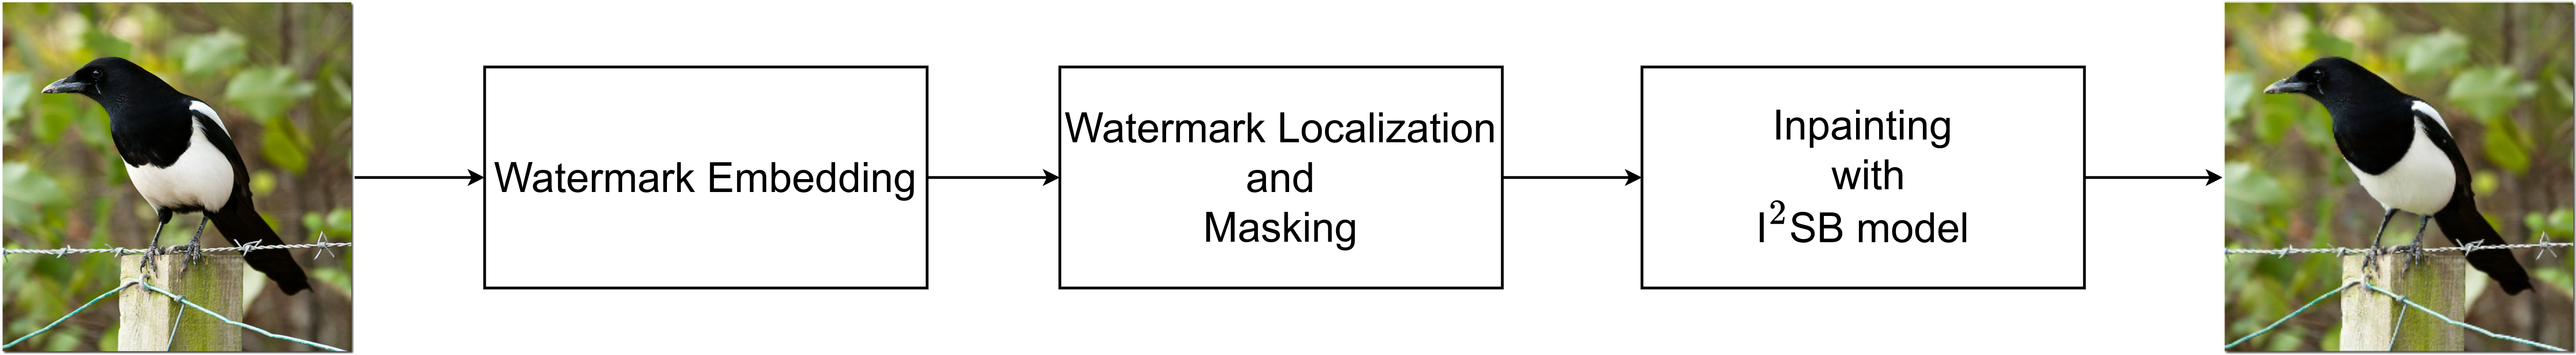
\includegraphics[width = \textwidth]{img/overall.png}
 \vspace{0.5cm}
 \caption{Overall pipeline for Watermark Attacking}
 \label{figure:overall_pipeline}
\end{figure}

% \begin{figure}[H]
%     \centering
%     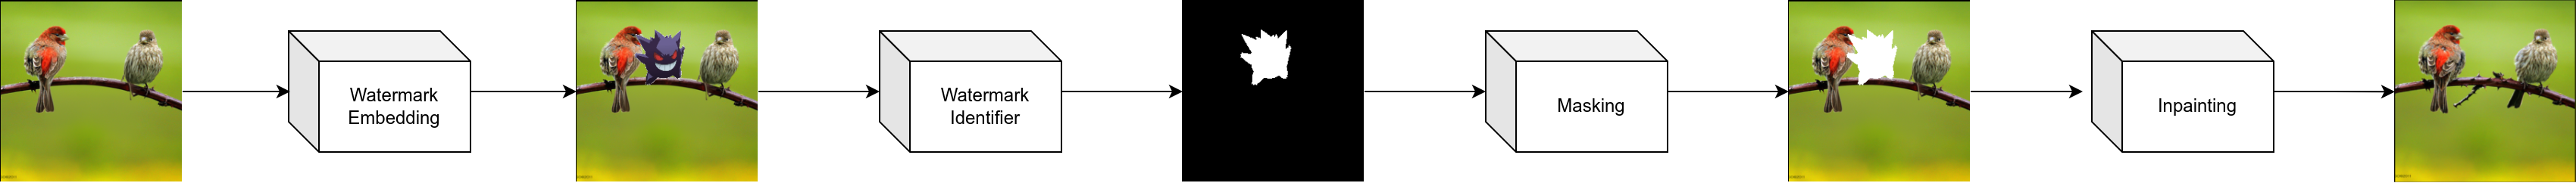
\includegraphics[width = \textwidth]{img/pipeline1.png}
%     
%     \caption{Approach 1}
%     \label{figure:appr1}
% \end{figure}

% \begin{figure}[H]
%     \centering
%     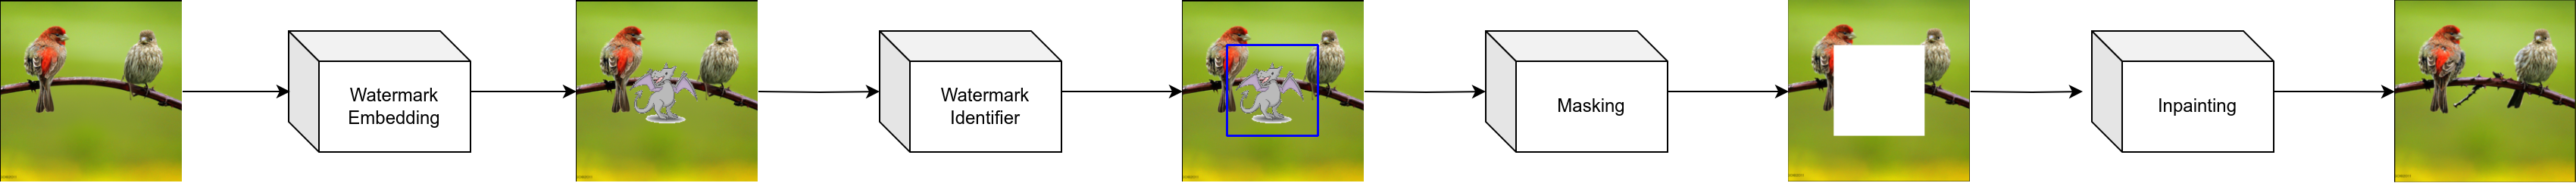
\includegraphics[width = \textwidth]{img/pipeline2.png}
%     
%     \caption{Approach 2}
%     \label{figure:appr2}
% \end{figure}
\subsection{Watermark Embedding}
\label{chapter:d:section:emb}
To begin, we will generate a watermarked dataset by embedding the watermark into the original images. Algorithm \ref{algorithm:embed} provides an overview of the watermark embedding process that we have implemented.
\begin{figure}[H]
 \centering
 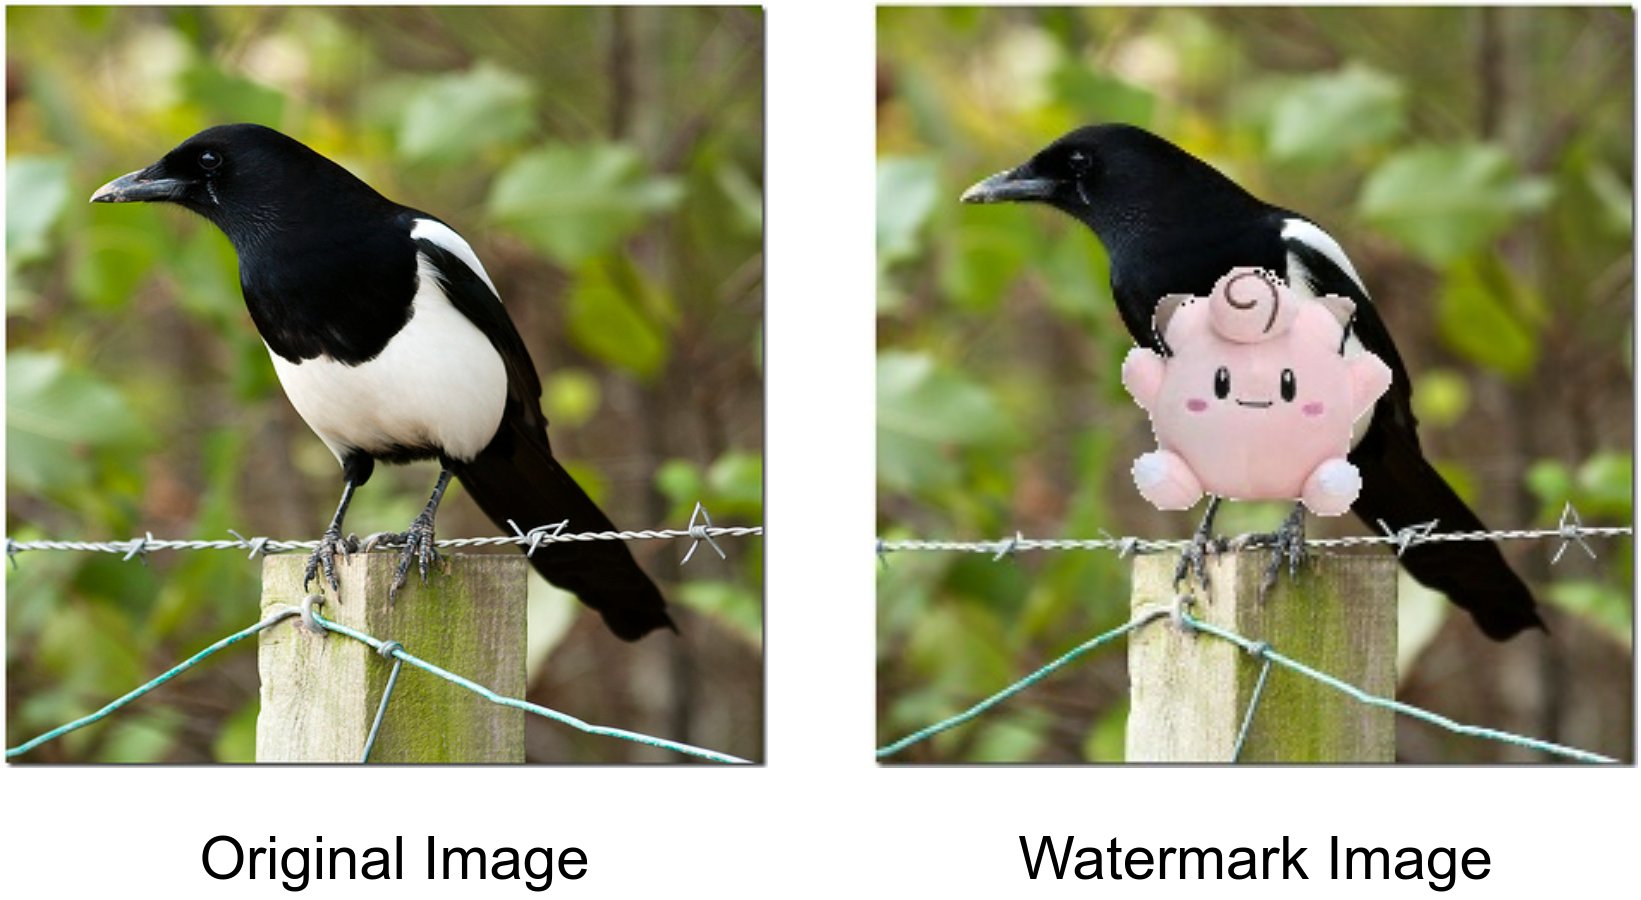
\includegraphics[width=0.75\linewidth]{img/embedded.png}

 \caption{Embed the watermark into image}
 \label{figure:embed_img}
\end{figure}
To embed the watermark, we begin with two datasets: one containing base images and the other comprising watermark images. For each image in the base dataset, we randomly select a watermark, extract its foreground using image processing, and extract the background by a specified color. For this step to be successful, it's crucial to choose a watermark dataset with minimal background detail.

The foreground of the watermark image is then placed onto the base image at a specified location, which can be either random or at the center of the image. After embedding the watermark, we save the watermarked image along with location information, such as bounding box or label map, for future reference. The resulting watermarked image is illustrated in Figure \ref{figure:embed_img}.
\begin{algorithm}[H]
 \caption{Embedding}
 \label{algorithm:embed}
 \begin{algorithmic}[1]
  \STATE {\bfseries Input:} clean dataset $A$ and watermark dataset $B$
  \FOR{$image$ {\bfseries in} $A$}
  \STATE Get random $sample$ from $B$
  \STATE Extract $foreground$ from $sample$
  \STATE Get $location$ to place watermark
  \STATE Place the $foreground$ on $location$ of $image$, save to $processed$
  \STATE Append $processed$ image to embedded dataset $C$
  \ENDFOR
  \STATE {\bfseries return} $C$
 \end{algorithmic}
\end{algorithm}
\subsection{Watermark Identifier}
After embedding and obtaining the watermarked dataset, the next step involves identifying its location information and subsequently masking it for the image inpainting task. Regarding the identifier, we plan to implement two approaches: Image Segmentation and Object Detection.
\subsubsection{Image Segmentation Approach}
In this approach, we aim to construct the watermark identifier as an object detection model. The pipeline for this approach is illustrated in Figure \ref{figure:segmentation}. There are various techniques for performing image segmentation, such as thresholding, clustering, region-based, edge-based, and graph-based methods. With the development of deep learning, many neural network architectures have been proposed for image segmentation tasks, such as U-Net, FastFCN, Gated-SCNN, and others. These architectures usually consist of an encoder and a decoder, where the encoder extracts features from the image and the decoder generates the segmentation mask. Some architectures also use additional modules or components, such as skip connections, attention mechanisms, or pyramid up-sampling, to improve the performance and accuracy of the segmentation
\begin{figure}[H]
 \centering
 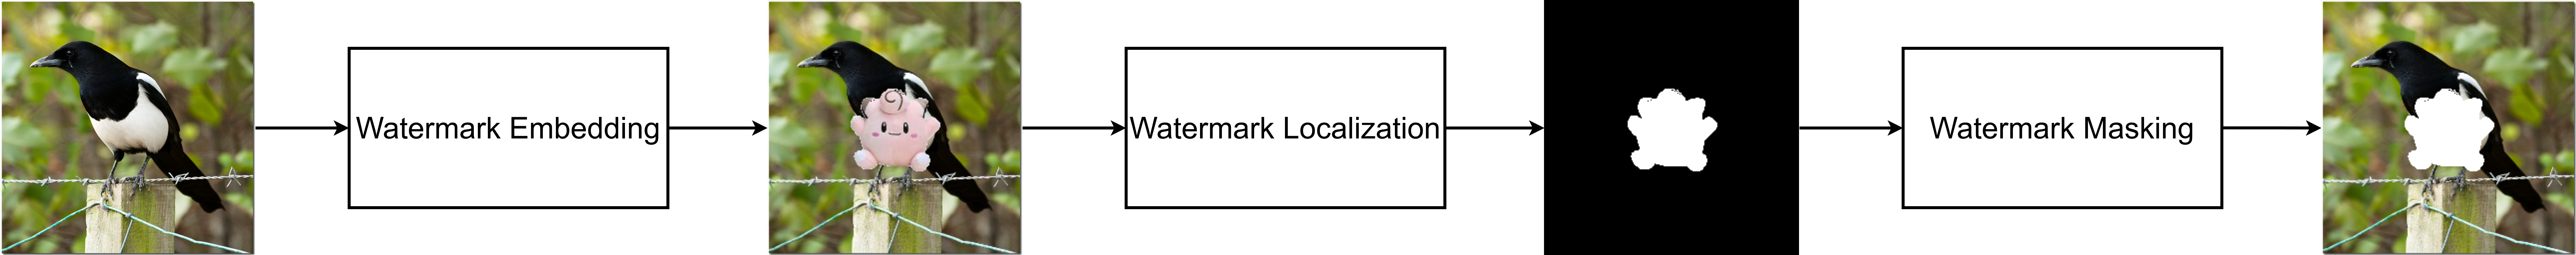
\includegraphics[width=\linewidth]{img/segmentation.png}

 \caption{Identify the watermark in image with Image Segmentation Approach}
 \label{figure:segmentation}
\end{figure}

The output of the image segmentation model is a segmentation map, with will extract the watermark out of the original image, as shown in the third image from left to right in Figure \ref{figure:segmentation}. The output from the segmentation approach provides a well-fitted segmentation for the watermark, ensuring that the mask precisely erases only the watermark during inpainting. This approach helps conserve the areas requiring inpainting, particularly those with intricate details. However, relying on segmentation introduces a strong dependency on the accuracy of the segmentation map. If the segmentation inaccurately fits the watermark, it may miss certain details, impacting the quality of the image after removing the watermark. Additionally, extending the segmentation map can be challenging, making it difficult to use the output if the watermark localization is incorrect.
\subsubsection{Object Detection Approach}
In this approach, we aim to construct the watermark identifier as an object detection model. The pipeline for this approach is illustrated in Figure \ref{figure:detection}. Object detection is a fundamental task in computer vision that aims to locate and classify objects in an image. Object detection methods can be broadly categorized into two types: two-stage detectors and one-stage detectors. Two-stage detectors first generate a set of region proposals that may contain objects, and then apply a classifier and a regressor to refine the proposals and predict the object labels and bounding boxes. One-stage detectors directly predict the object labels and bounding boxes for all the pixels or anchors in the image, without using region proposals.

Two-stage detectors are usually more accurate than one-stage detectors, but also slower and more complex. The most representative two-stage detector is the R-CNN family, which includes R-CNN, Fast R-CNN, and Faster R-CNN. R-CNN extracts features from each region proposal using a convolutional neural network (CNN), and then uses a support vector machine (SVM) and a linear regressor to classify and localize the objects. Fast R-CNN improves R-CNN by sharing the CNN features among all the region proposals, and using a softmax classifier and a bounding box regressor instead of SVM and linear regressor. Faster R-CNN further improves Fast R-CNN by replacing the selective search algorithm for generating region proposals with a region proposal network (RPN), which is a fully convolutional network that can be trained end-to-end with the detection network.

One-stage detectors are usually faster than two-stage detectors, but also less accurate and more prone to false positives. The most representative one-stage detector is the YOLO family, which now release up to YOLOv8. YOLO divides the input image into a grid of cells, and predicts the object labels and bounding boxes for each cell.

Moreover, some recent object detection methods try to bridge the gap between two-stage and one-stage detectors, by combining the advantages of both types. For example, RetinaNet  is a one-stage detector that introduces a focal loss function to address the class imbalance problem, which is the main cause of the lower accuracy of one-stage detectors. DERT  is a two-stage detector that uses a dynamic and efficient region transformer to generate adaptive region proposals, which can reduce the computation and memory cost of the detection network.
\begin{figure}[H]
 \centering
 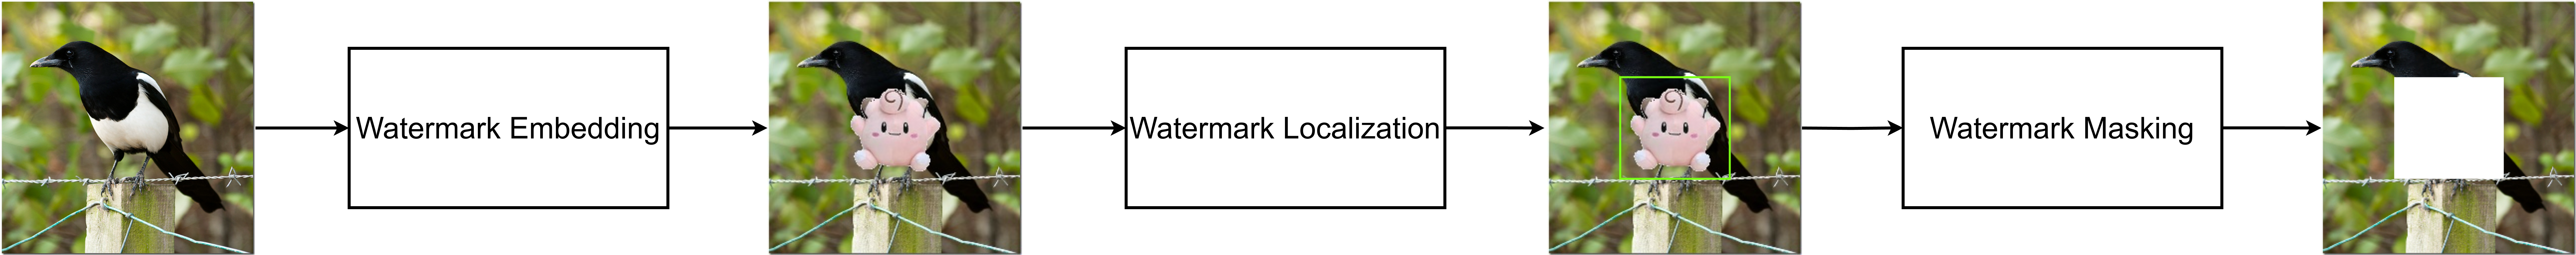
\includegraphics[width=\linewidth]{img/detection.png}

 \caption{Identify the watermark in image with Object Detection Approach}
 \label{figure:detection}
\end{figure}

The output of the object detection model is a bounding box, indicating the rectangular area where the watermark is located. Consequently, the masking area, once the box is determined, may be larger than the watermark itself. This can result in the inpainting task having to restore a larger masked area compared to the segmentation approach. However, with the location provided by the bounding box, the model's error rate may be lower than that of segmentation. This is because the segmentation approach needs to predict the exact structure of the watermark, which could be prone to missing some details.

Moreover, with the bounding box, we have the flexibility to add a padding size to the box if needed. On the contrary, extending the segmentation map can be challenging. In summary, the object detection approach makes it easier to accurately detect the location of the watermark, but the larger bounding box may pose challenges for the inpainting task.

In summary of this section, within the scope of this project, we have not yet developed a watermark identifier due to time constraints. Consequently, to execute this pipeline, we leverage the saved watermark labeling information, as discussed in Section \ref{chapter:d:section:emb}. This information is utilized for masking, enabling us to proceed directly to the image inpainting task. The development of the watermark identifier will be continued in the next phase of this project.
\subsection{Image Inpainting}
Finally, after obtaining a masked image by applying the detected watermark mask, we proceed with the inpainting task. For this task, we employ the I$^2$SB model to inpaint the masked region in the image. The process is illustrated in Figure \ref{figure:inpainting_arch}.
\begin{figure}[H]
 \centering
 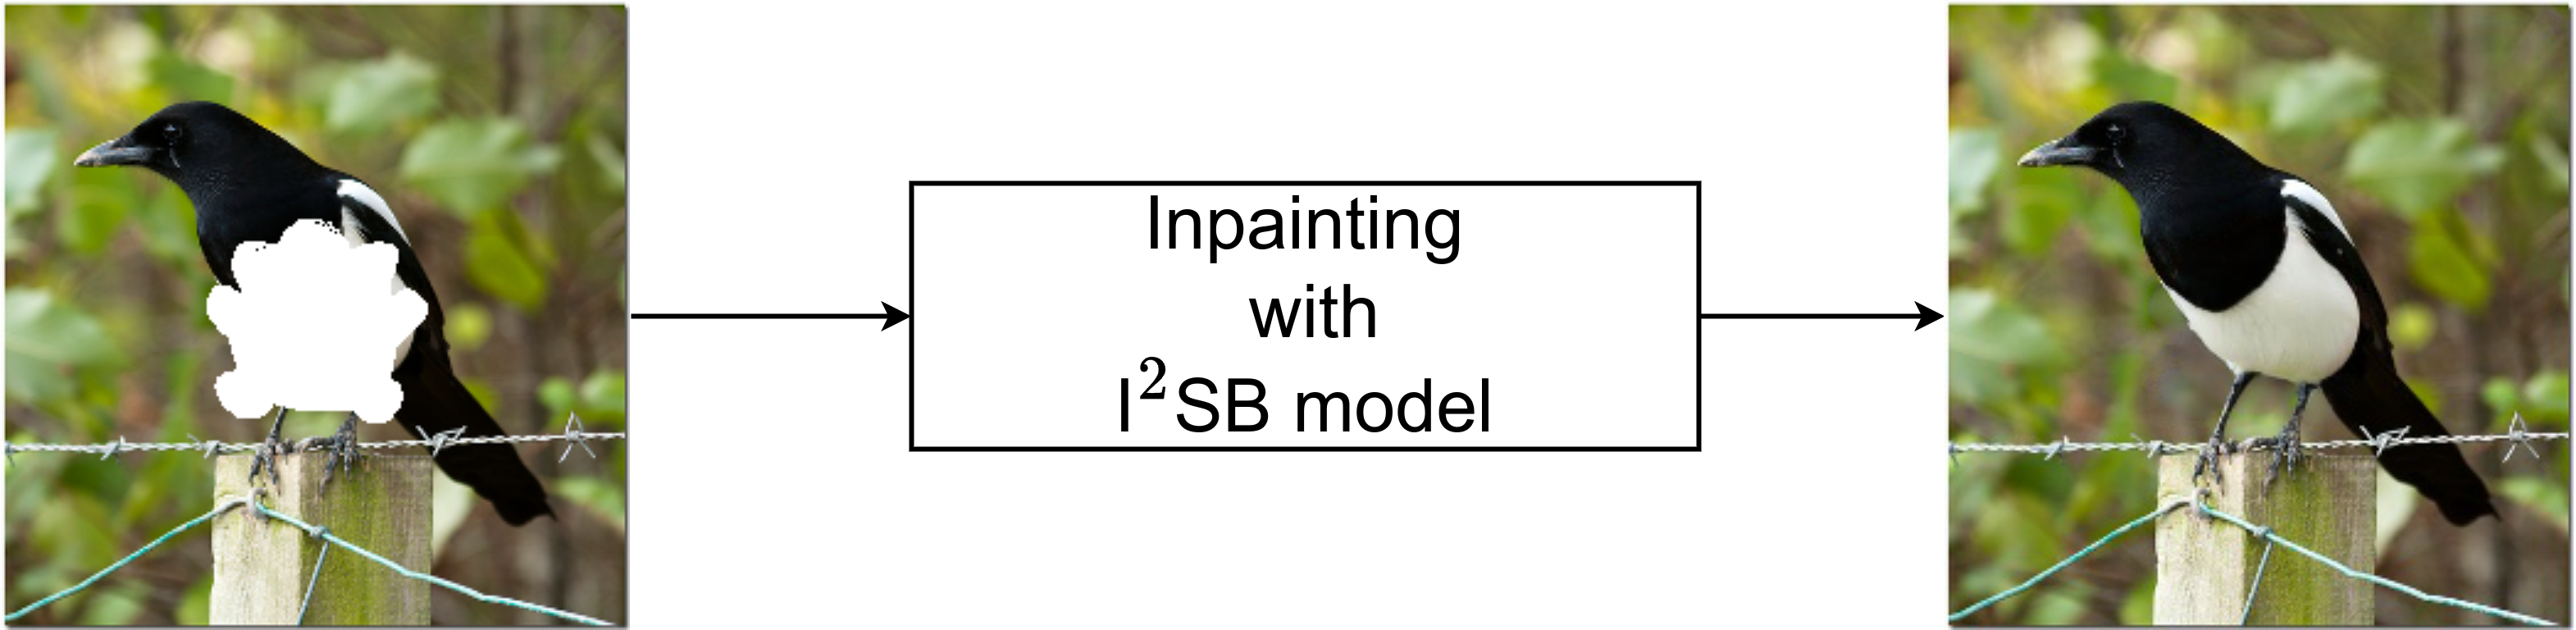
\includegraphics[width=0.75\linewidth]{img/inpainting_arch.png}

 \caption{Inpainting the mask image with I$^2$SB}
 \label{figure:inpainting_arch}
\end{figure}
The process of inpainting is explained in Figure \ref{figure:inpainting_arch}. We work with a set of details that include both the original and the covered-up image. From this information, we pick out the part of the image that's covered. The aim of this inpainting task is to bring back the covered section we've identified, hoping to recreate an image that closely resembles the original one.
\chapter{Proposed Method and Experiments}
\label{chap:experiment}
\thispagestyle{empty}
In this chapter, we will propose a diffusion-based pipeline for watermark removal. We will then focus on conducting experiments using the proposed pipeline for watermark removal, as detailed in Section \ref{sec:pipeline}. The experiments utilize the ImageNet dataset, with the Pokémon dataset serving as the watermark. Further information about the datasets will be provided in Section \ref{sec:dataset}. The results of our pipeline, from watermark embedding to removal and image inpainting, will be presented step by step. Section \ref{sec:removal} will discuss the outcomes in detail.

Upon completing all experiments, we aim to establish metrics for evaluation. Section \ref{sec:metrics} will provide a comprehensive discussion on these metrics, offering an overview and assisting in selecting the most suitable metric to assess the effectiveness of our pipeline in watermark removal.
% Summary experiments:
% proposed pipeline done + result + masks position
% datasets
% metrics

\section{Proposed Watermark Attacking Pipeline}
\label{sec:pipeline}
As backgrounds and methodologies relevant to the Watermark Attacking problem have been clarified, in this section we introduce our proposed pipeline designed to address this challenge. Figure \ref{figure:overall_pipeline} provides an overview of our comprehensive pipeline, encompassing the following steps
\begin{enumerate}
 \item The original image undergoes Watermark Embedding through the Watermark Embedder. The watermark information for each image is also stored for later evaluation.
 \item The watermarked image then passes through a Watermark Localization model, revealing regional information of the watermark. The watermark is then masked from the image, creating a degraded image to be inpainted.
 \item Finally, the inpainting process, specifically I$^2$SB in our case, reconstructs the image to closely resemble the original image.
\end{enumerate}
\begin{figure}[t]
 \centering
 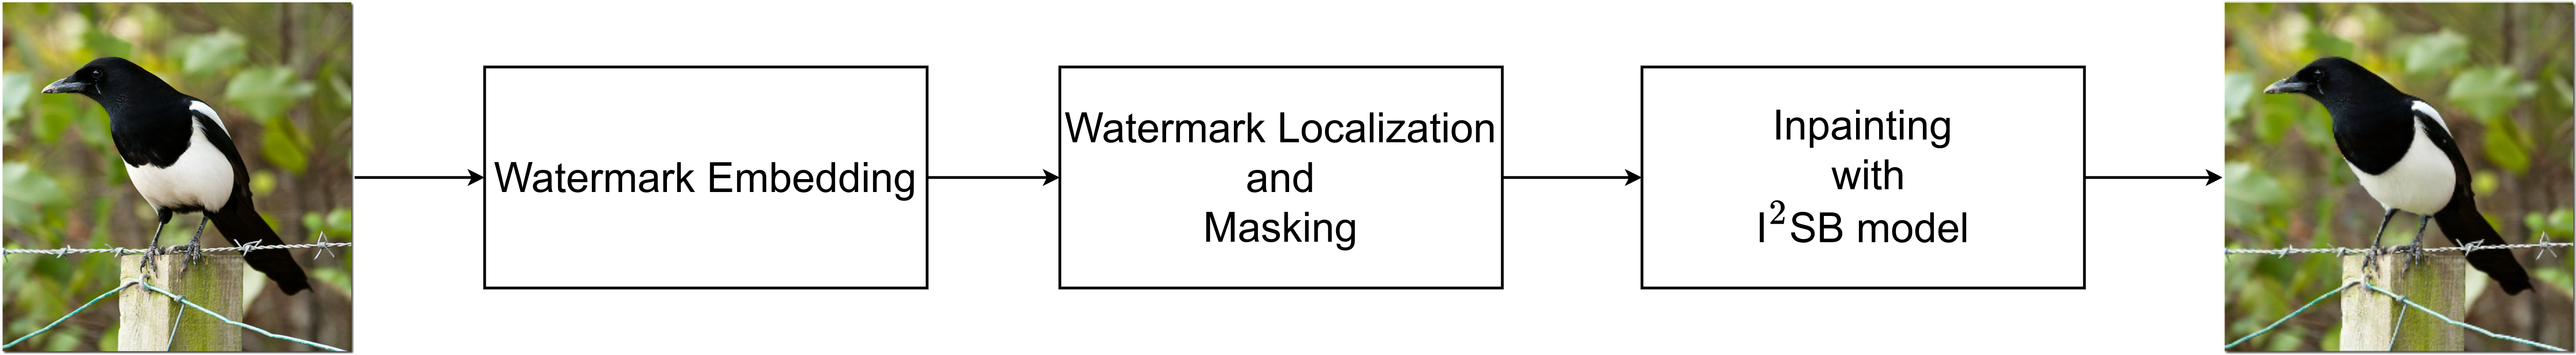
\includegraphics[width = \textwidth]{img/overall.png}
 %\vspace{0.5cm}
 \caption{Overall pipeline for Watermark Attacking}
 \label{figure:overall_pipeline}
\end{figure}

% \begin{figure}[t]
%     \centering
%     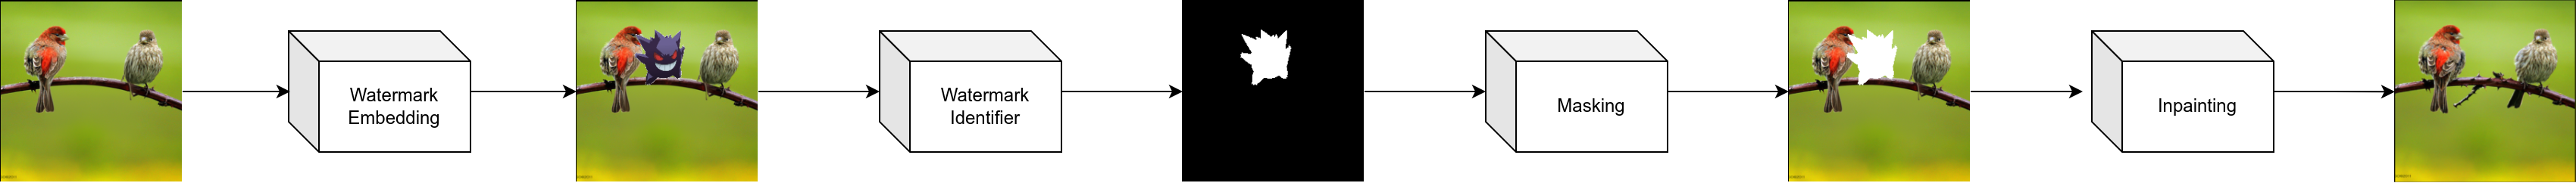
\includegraphics[width = \textwidth]{img/pipeline1.png}
%     
%     \caption{Approach 1}
%     \label{figure:appr1}
% \end{figure}

% \begin{figure}[t]
%     \centering
%     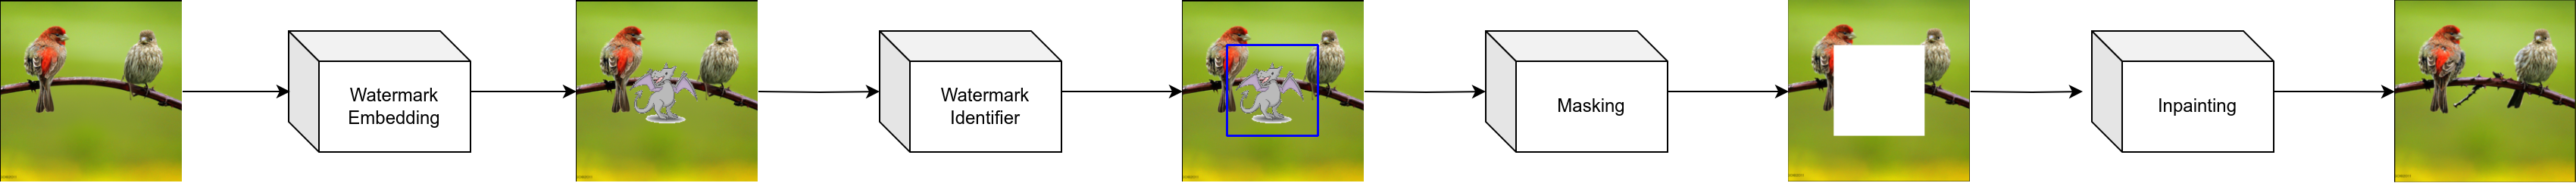
\includegraphics[width = \textwidth]{img/pipeline2.png}
%     
%     \caption{Approach 2}
%     \label{figure:appr2}
% \end{figure}
\subsection{Watermark Embedding}
\label{chapter:d:section:emb}
To begin, we will generate a watermarked dataset by embedding the watermark into the original images. Algorithm \ref{algorithm:embed} provides an overview of the watermark embedding process that we have implemented.
\begin{figure}[t]
    \centering
    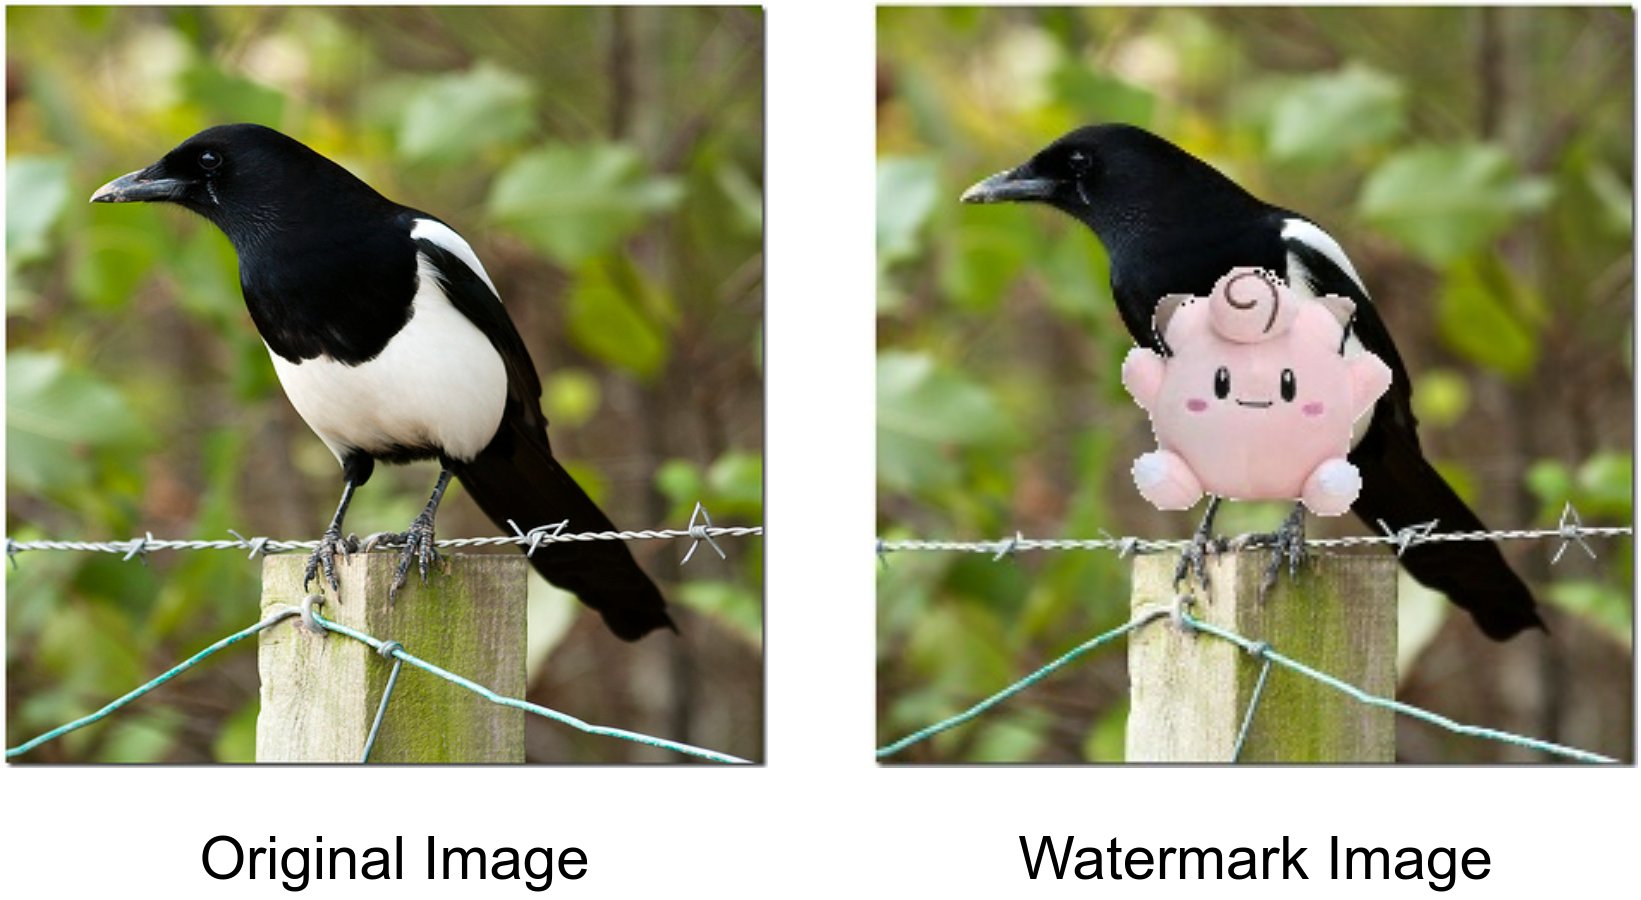
\includegraphics[width=0.75\linewidth]{img/embedded.png}
    %\vspace{0.5cm}
    \caption{Embed a watermark into the image}
    \label{figure:embed_img}
\end{figure}
To embed the watermark, we begin with two datasets: one containing base images and the other comprising watermark images. For each image in the base dataset, we randomly select a watermark, extract its foreground using image processing, and extract the background by a specified color. For this step to be successful, it is crucial to choose a watermark dataset with minimal background detail.

The foreground of the watermark image is then placed onto the base image at a specified location, which can be either random or at the center of the image. After embedding the watermark, we save the watermarked image along with location information, such as bounding box or label map, for future reference. The resulting watermarked image is illustrated in Figure \ref{figure:embed_img}.
\begin{algorithm}[t]
 \caption{Embedding}
 \label{algorithm:embed}
 \begin{algorithmic}[1]
  \STATE {\bfseries Input:} clean dataset $A$ and watermark dataset $B$
  \FOR{$image$ {\bfseries in} $A$}
  \STATE Get random $sample$ from $B$
  \STATE Extract $foreground$ from $sample$
  \STATE Get $location$ to place watermark
  \STATE Place the $foreground$ on $location$ of $image$, save to $processed$
  \STATE Append $processed$ image to embedded dataset $C$
  \ENDFOR
  \STATE {\bfseries return} $C$
 \end{algorithmic}
\end{algorithm}
\subsection{Watermark Localization}
After embedding and obtaining the watermarked dataset, the next step involves identifying its location information and subsequently masking it for the image inpainting task. Regarding the identifier, we consider two approaches: Image Segmentation and Object Detection.
\subsubsection{Image Segmentation Approach}
In this approach, we aim to construct the watermark identifier as an object detection model. The pipeline for this approach is illustrated in Figure \ref{figure:segmentation}. There are various techniques for performing image segmentation, such as thresholding, clustering, region-based, edge-based, and graph-based methods. With the development of deep learning, many neural network architectures have been proposed for image segmentation tasks, such as U-Net, FastFCN \cite{wu2019fastfcn}, Gated-SCNN \cite{takikawa2019gated}, and others. These architectures usually consist of an encoder and a decoder, where the encoder extracts features from the image and the decoder generates the segmentation mask. Some architectures also use additional modules or components, such as skip connections, attention mechanisms, or pyramid up-sampling, to improve the performance and accuracy of the segmentation
\begin{figure}[t]
 \centering
 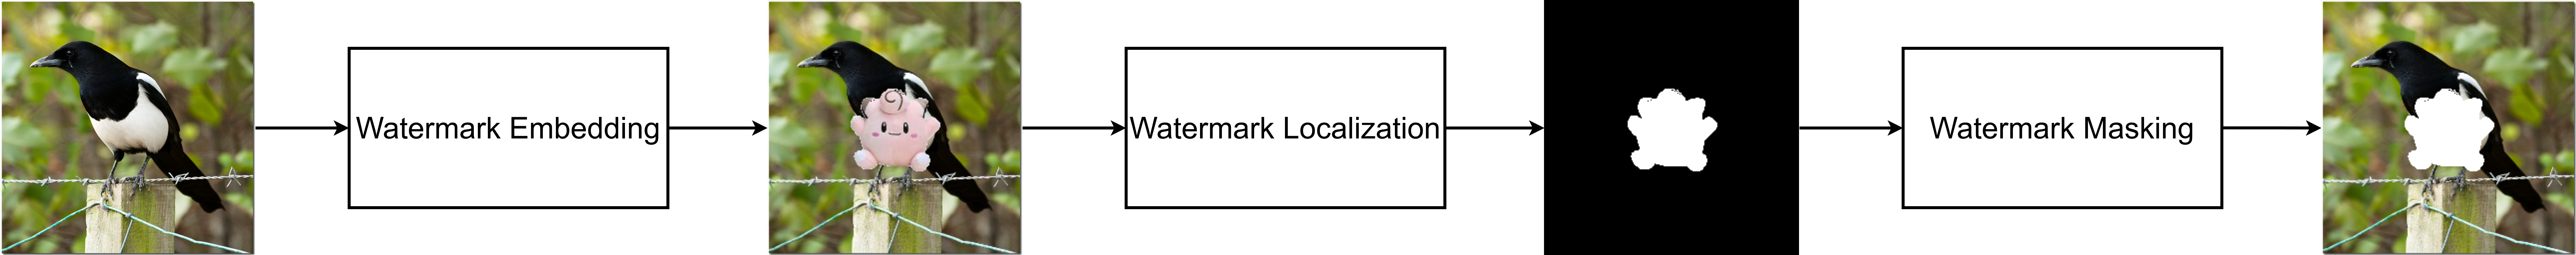
\includegraphics[width=\linewidth]{img/segmentation.png}
 %\vspace{0.5cm}
 \caption{Identify the watermark in image with Image Segmentation Approach}
 \label{figure:segmentation}
\end{figure}

The output of the image segmentation model is a segmentation map, with will extract the watermark out of the original image, as shown in the third image from left to right in Figure \ref{figure:segmentation}. The output from the segmentation approach provides a well-fitted segmentation for the watermark, ensuring that the mask precisely erases only the watermark during inpainting. This approach helps conserve the areas requiring inpainting, particularly those with intricate details. However, relying on segmentation introduces a strong dependency on the accuracy of the segmentation map. If the segmentation inaccurately fits the watermark, it may miss certain details, impacting the quality of the image after removing the watermark. Additionally, extending the segmentation map can be challenging, making it difficult to use the output if the watermark localization is incorrect.
\subsubsection{Object Detection Approach}
In this approach, we aim to construct the watermark identifier as an object detection model. The pipeline for this approach is illustrated in Figure \ref{figure:detection}. Object detection is a fundamental task in computer vision that aims to locate and classify objects in an image. Object detection methods can be broadly categorized into two types: two-stage detectors and one-stage detectors. Two-stage detectors first generate a set of region proposals that may contain objects, and then apply a classifier and a regressor to refine the proposals and predict the object labels and bounding boxes. One-stage detectors directly predict the object labels and bounding boxes for all the pixels or anchors in the image, without using region proposals.

Two-stage detectors are usually more accurate than one-stage detectors, but also slower and more complex. The most representative two-stage detector is the R-CNN family, which includes R-CNN \cite{girshick2014rich}, Fast R-CNN \cite{girshick2015fast}, and Faster R-CNN  \cite{ren2016faster}. R-CNN extracts features from each region proposal using a convolutional neural network (CNN), and then uses a support vector machine (SVM) and a linear regressor to classify and localize the objects. Fast R-CNN improves R-CNN by sharing the CNN features among all the region proposals, and using a softmax classifier and a bounding box regressor instead of SVM and linear regressor. Faster R-CNN further improves Fast R-CNN by replacing the selective search algorithm for generating region proposals with a region proposal network (RPN), which is a fully convolutional network that can be trained end-to-end with the detection network.

One-stage detectors are usually faster than two-stage detectors, but also less accurate and more prone to false positives. The most representative one-stage detector is the YOLO \cite{redmon2016you} family, which now release up to YOLOv8. YOLO divides the input image into a grid of cells, and predicts the object labels and bounding boxes for each cell.

Moreover, some recent object detection methods try to bridge the gap between two-stage and one-stage detectors, by combining the advantages of both types. For example, RetinaNet \cite{lin2017focal} is a one-stage detector that introduces a focal loss function to address the class imbalance problem, which is the main cause of the lower accuracy of one-stage detectors. DERT \cite{carion2020end} is a two-stage detector that uses a dynamic and efficient region transformer to generate adaptive region proposals, which can reduce the computation and memory cost of the detection network.
\begin{figure}[t]
 \centering
 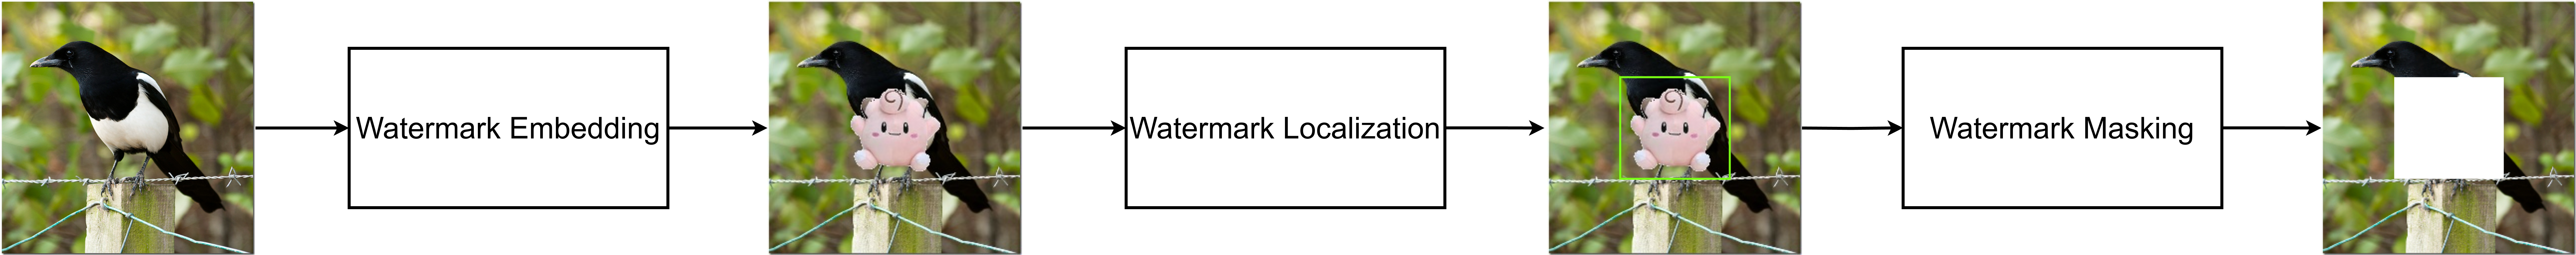
\includegraphics[width=\linewidth]{img/detection.png}
 % %\vspace{0.5cm}

 \caption{Identify the watermark in image with Object Detection Approach}
 \label{figure:detection}
\end{figure}

The output of the object detection model is a bounding box, indicating the rectangular area where the watermark is located. Consequently, the masking area, once the box is determined, may be larger than the watermark itself. This can result in the inpainting task having to restore a larger masked area compared to the segmentation approach. However, with the location provided by the bounding box, the model's error rate may be lower than that of segmentation. This is because the segmentation approach needs to predict the exact structure of the watermark, which could be prone to missing some details.

Moreover, with the bounding box, we have the flexibility to add a padding size to the box if needed. On the contrary, extending the segmentation map can be challenging. In summary, the object detection approach makes it easier to accurately detect the location of the watermark, but the larger bounding box may pose challenges for the inpainting task.

% In summary of this section, within the scope of this project, we have not yet developed a watermark identifier due to time constraints. Consequently, to execute this pipeline, we leverage the saved watermark labeling information, as discussed in Section \ref{chapter:d:section:emb}. This information is utilized for masking, enabling us to proceed directly to the image inpainting task. The development of the watermark identifier will be continued in the next phase of this project.
\subsection{Image Inpainting}
Finally, after obtaining a masked image by applying the detected watermark mask, we proceed with the inpainting task. For this task, we employ the I$^2$SB model to inpaint the masked region in the image. The process is illustrated in Figure \ref{figure:inpainting_arch}.
\begin{figure}[t]
 \centering
 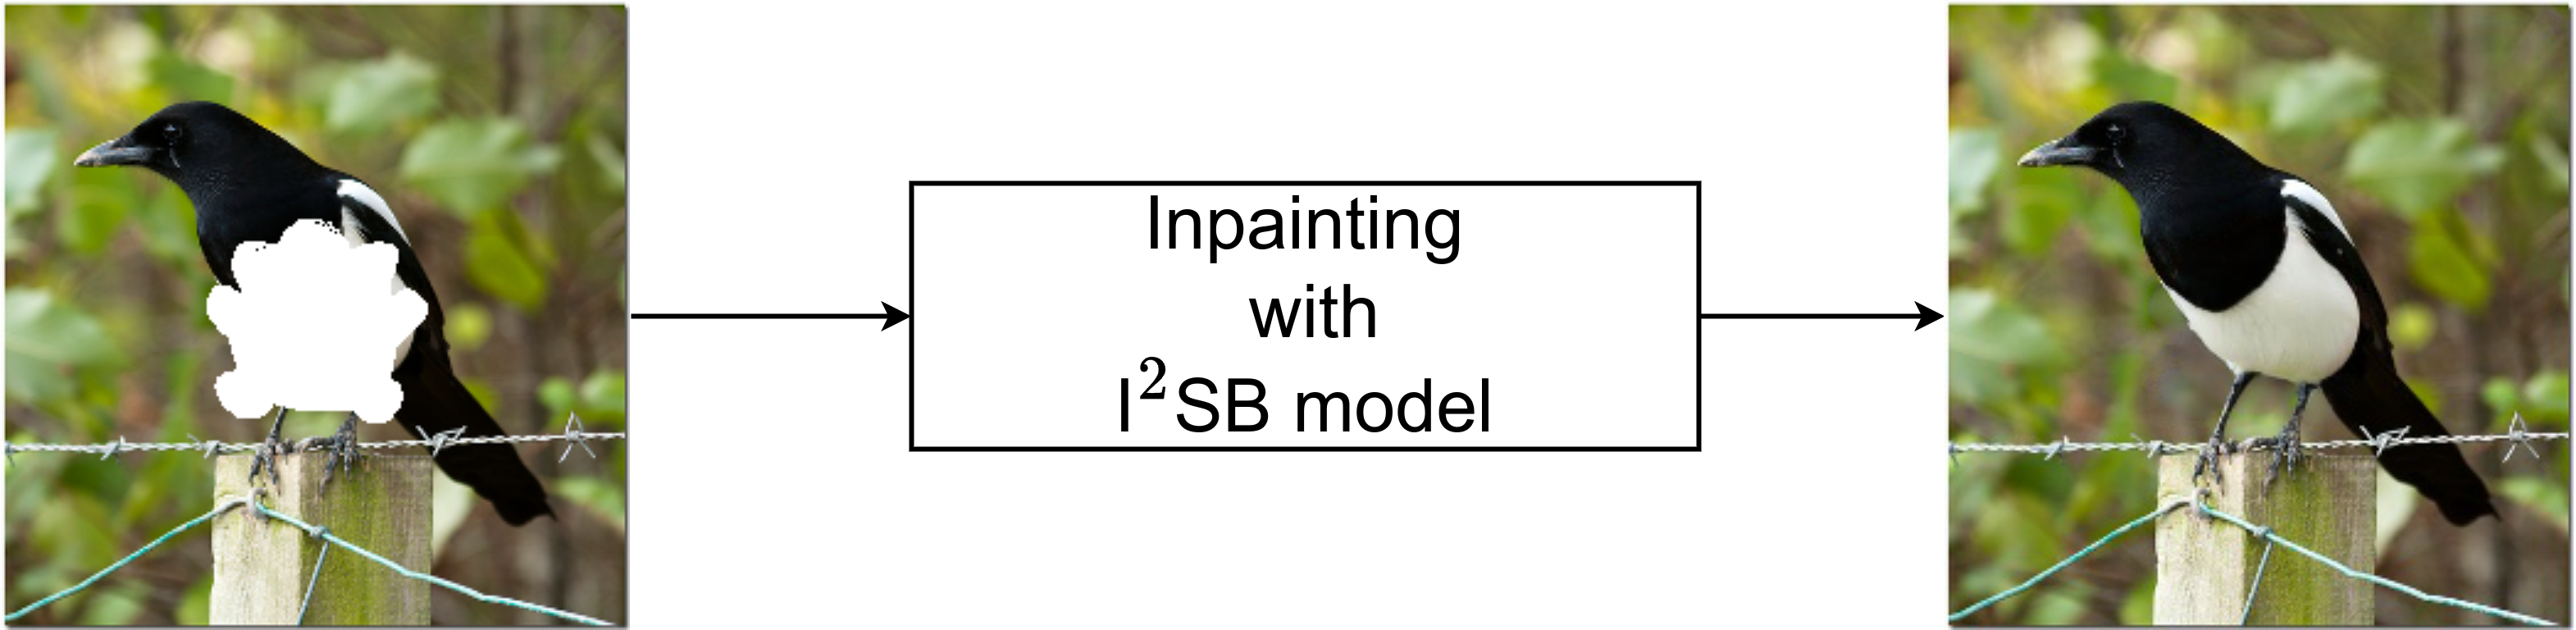
\includegraphics[width=0.75\linewidth]{img/inpainting_arch.png}
 %\vspace{0.5cm}

 \caption{Inpainting the mask image with I$^2$SB}
 \label{figure:inpainting_arch}
\end{figure}
The process of inpainting is explained in Figure \ref{figure:inpainting_arch}. We work with a set of details that include both the original and the covered-up image. From this information, we pick out the part of the image that is covered. The aim of this inpainting task is to bring back the covered section we have identified, hoping to recreate an image that closely resembles the original one.

\section{Datasets}
\label{sec:dataset}
\subsection{Image Dataset}
\label{sec:dataset:clean}

We start conducting the experiments on our pipeline by choosing a dataset as the starting point for our work, where we will add watermarks and later remove them. Since we are planning to use the I$^2$SB model, and reproducing the training on other datasets is a bit tricky due to limited resources, we decide to go with a dataset where the model has already been trained. The I$^2$SB model is primarily trained on ImageNet with an image size of $256 \times 256$ for the task of image inpainting. Therefore, we will be using ImageNet as our primary dataset for the upcoming experiments. Additionally, we will carry out experiments in the image inpainting task using the ImageNet 10k validation subset, which comprises approximately 10,000 samples.

\subsection{Watermark Dataset}
\label{sec:dataset:wtm}
For the watermark dataset, we choose a dataset with minimal background detail. Therefore, we choose a dataset we discovered on Kaggle named \textit{Pokémon from First Gen}\footnote{\href{https://www.kaggle.com/datasets/unexpectedscepticism/11945-pokemon-from-first-gen}{Pokemon from First Gen Dataset, Kaggle}}. This dataset comprises approximately 12,000 samples of Pokémon characters, all featuring a white or transparent background. This simplicity makes it easier for us to embed these characters into the original images. You can view samples from this dataset in Figure \ref{fig:Pokemon}.

\begin{figure}[t]
    \centering
    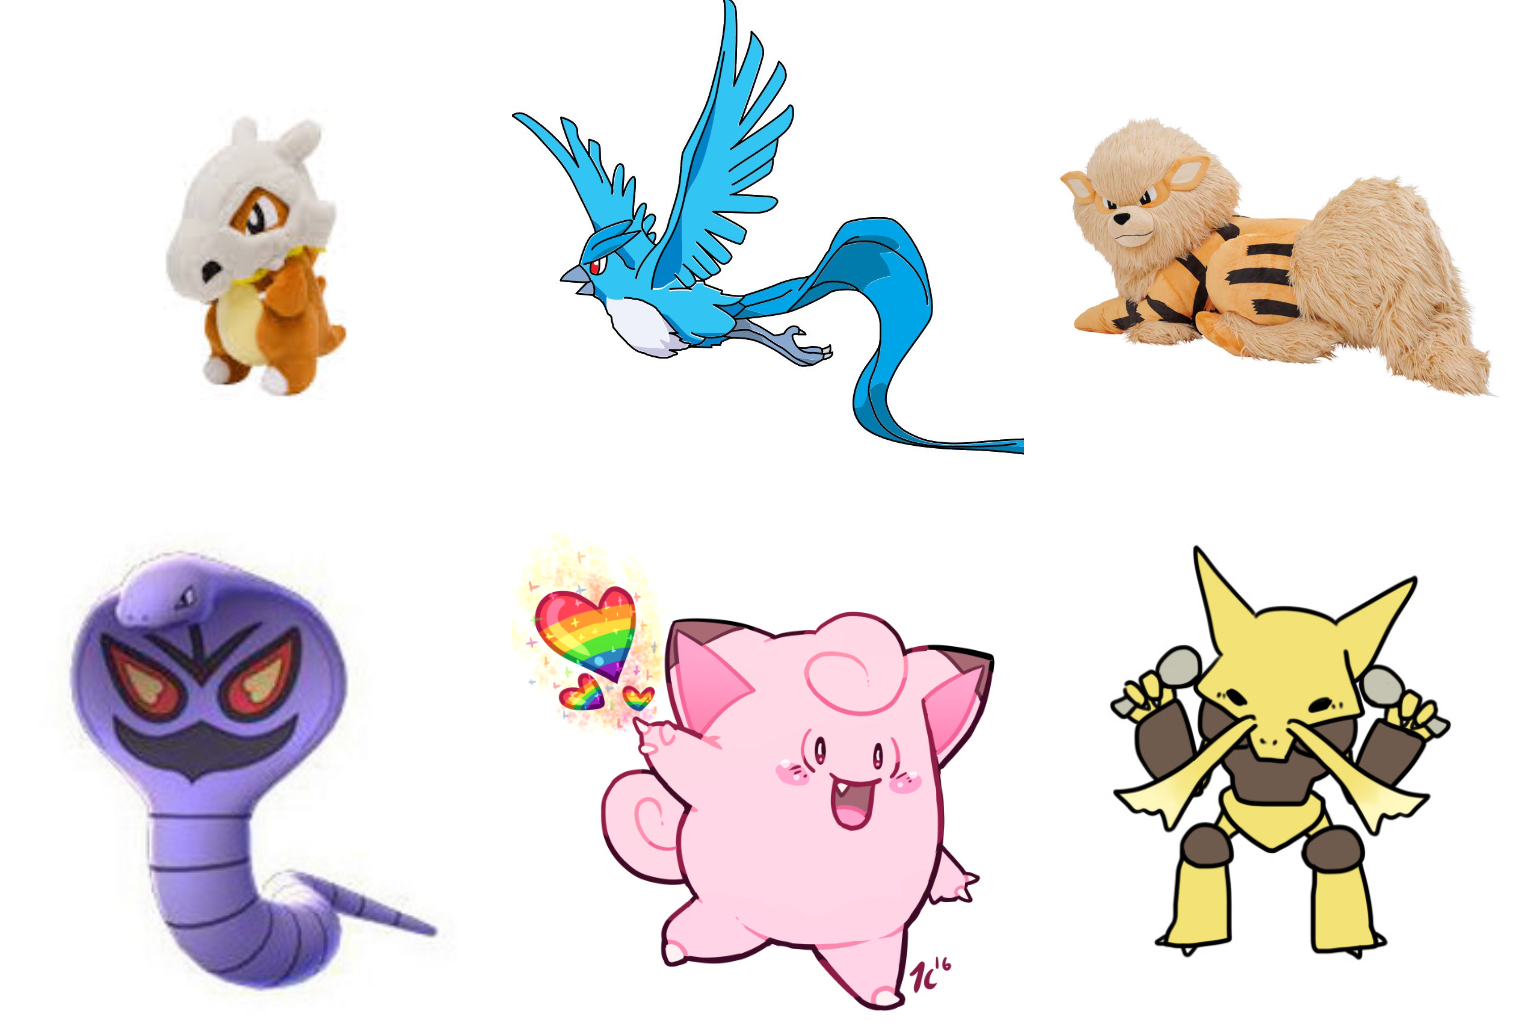
\includegraphics[width = 0.5 \textwidth]{img/Pokemon.png}
    %\vspace{0.5cm}
    \caption{Watermark Dataset}
    \label{fig:Pokemon}
\end{figure}

\subsection{Embedded Watermark Image}
% \textcolor{red}{Move to dataset for watermarked image dataset}
\label{sec:ewi}
\label{sec:embedding}
In this section, we will conduct experiments on embedding the watermarks into images. Our goal is to create a dataset of watermarked images that can later be used to attack the watermark. We performed watermark embedding on the ImageNet dataset as mentioned in Section \ref{sec:dataset:clean}. Samples of this dataset are illustrated in the first row of Figure \ref{fig:watermark-embedding}.

\begin{figure}[t]
    \centering
    \includegraphics[width=0.8\linewidth]{img/watermark-embedding.png}
    \caption{Watermark embedding and its positional information}
    \label{fig:watermark-embedding}
\end{figure}

To embed the watermark, we need a watermark dataset as mentioned in Section \ref{sec:dataset:wtm}. The watermark images we choose have a white background, making it easier to separate the object from the background using image processing techniques. Since image pixels are represented by values ranging from 1 to 255, the white background has a value of 255 across all its channels (RGB). We create a mask by assigning a value of 1 to pixels that differ from 255, and a value of 0 to pixels with the value of 255. This mask effectively isolates the watermark object from its background, making it ready to be embedded into the target image. The Figure \ref{fig:wtm-obj-mask-1} illustrates the watermark image and its corresponding mask, which labels the watermark object.

\begin{figure}[t]
    \centering
    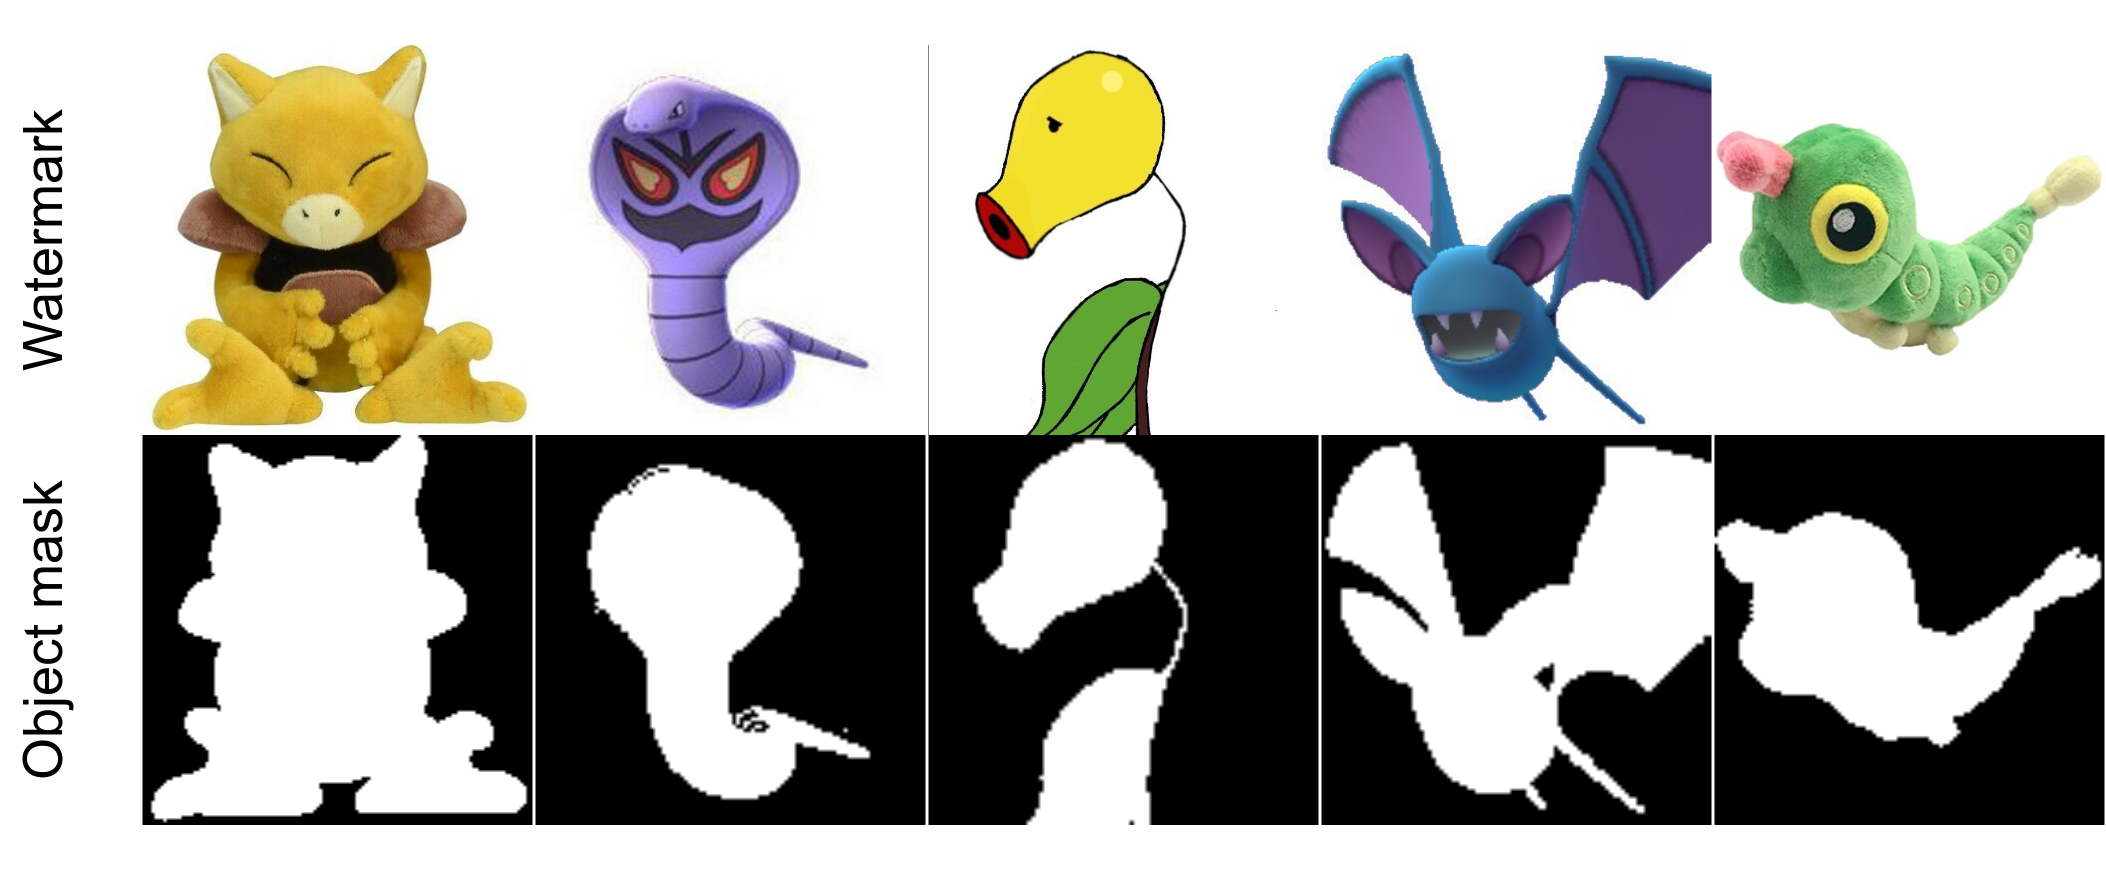
\includegraphics[width=0.8\linewidth]{img/watermark-and-objectmask.png}
    %\vspace{0.5cm}
    \caption{Watermark image and its object mask}
    \label{fig:wtm-obj-mask-1}
\end{figure}

Sometimes, however, the watermark object itself has pixel values of 255 across all its channels (RGB), causing the mask to fail, as shown in the first and second row of Figure \ref{fig:wtm-with-white-detail}. To handle this case, we need to use a morphological image processing method called Closing. This method will connect the black holes in the object mask and ensure that the white areas within the object are included in the mask, as shown in the last row of Figure \ref{fig:wtm-with-white-detail}.

\begin{figure}[t]
    \centering
    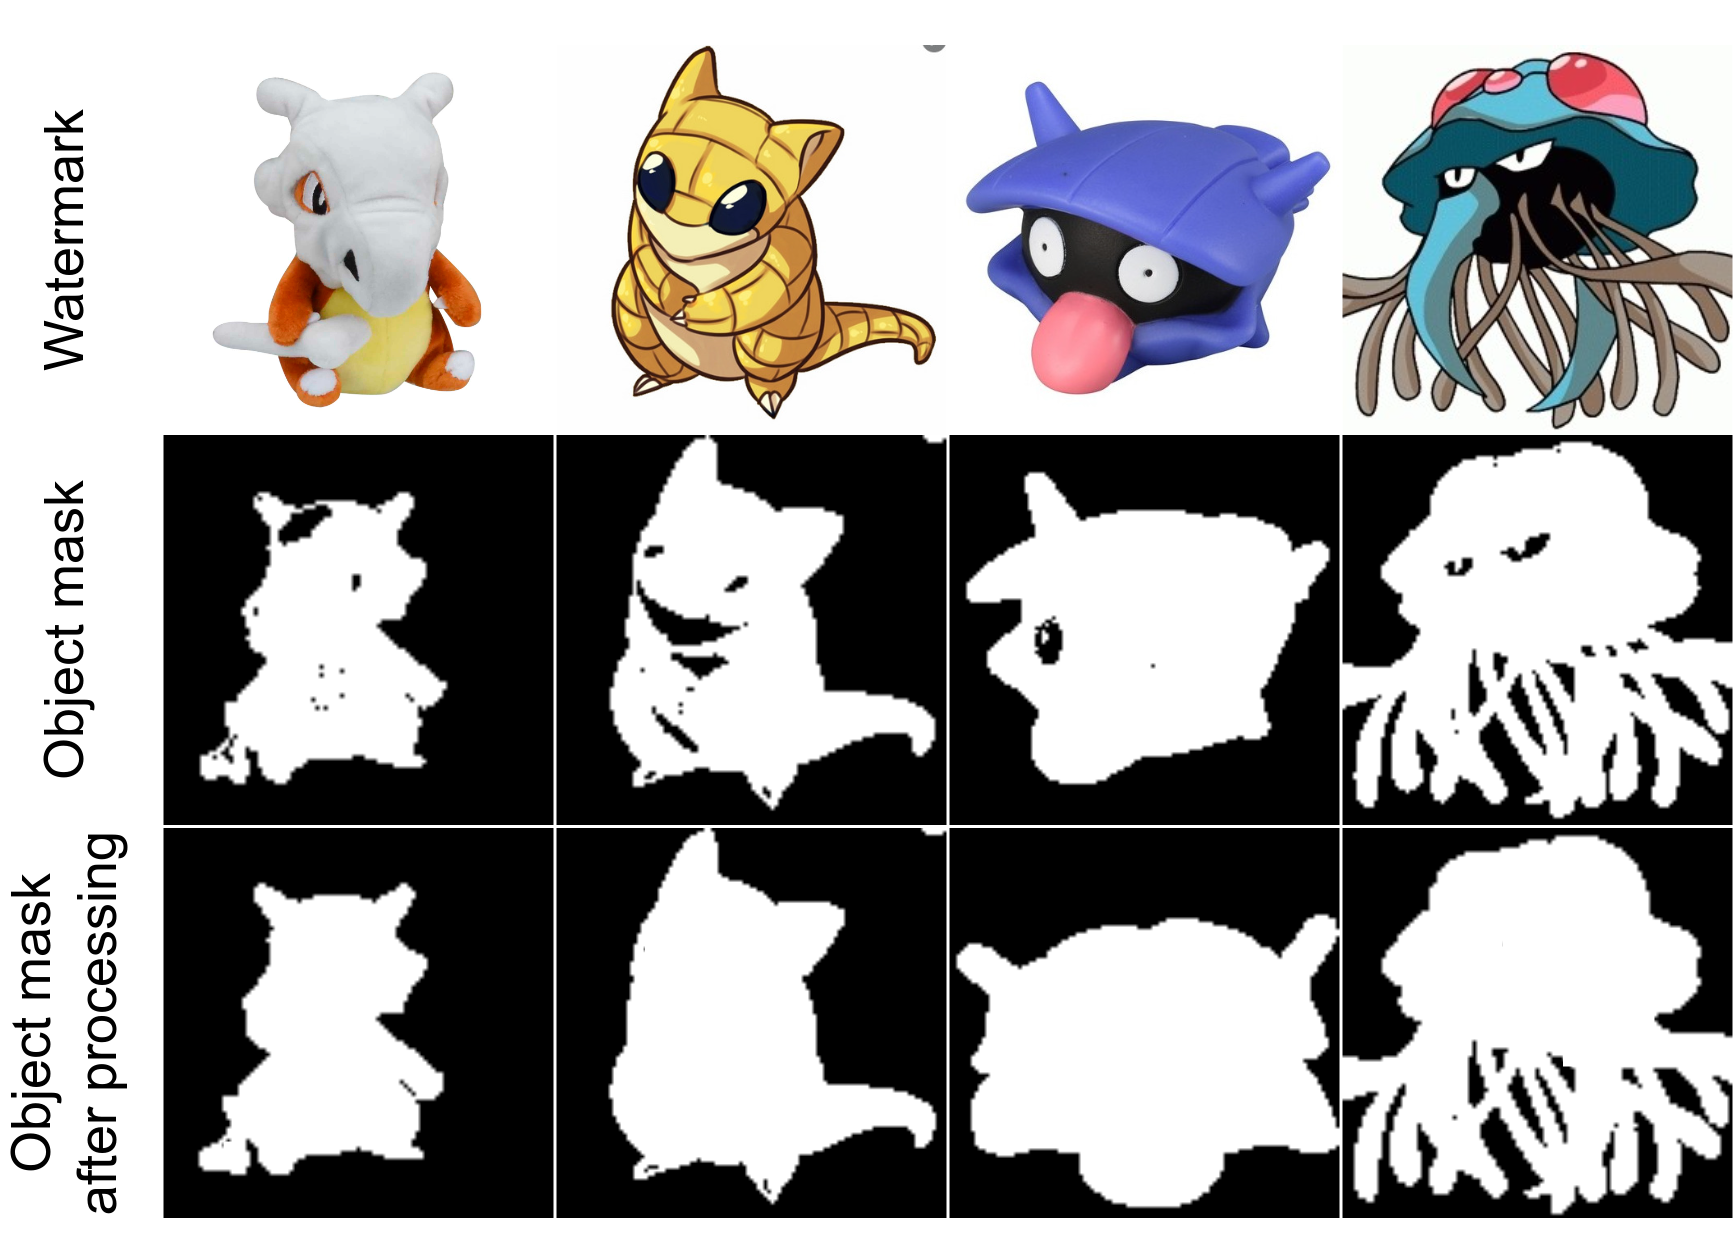
\includegraphics[width=0.8\linewidth]{img/wtm_embed_processing.png}
    %\vspace{0.5cm}
    \caption[Watermark image morphological image processing methods]{Watermark image that its object have white detail and its post-processing by using morphological image processing methods}
    \label{fig:wtm-with-white-detail}
\end{figure}

In addition, some images in the watermark dataset have transparency, which includes a fourth channel for opacity. These images indicate the opacity of the watermark object with a value of 1, meaning fully visible, and the background with a value of 0, meaning fully invisible. In this case, we can separate the watermark object from its background by creating a mask that matches the values of the opacity channel. Then, we reduce these watermark images to the usual three channels (RGB) for convenience in processing.

The watermark object now is ready to embed, we then choose a location in the original image to place the watermark. This is done by selecting a point that marks where the top-left corner of the watermark image will be positioned on the original image. After that, we paste the entire watermark image, ensuring that the top-left corner aligns with the chosen point. The size of the watermark image will be constrained to cover 10-30\% of the original image area. Additionally, we adjust the opacity of the watermark to vary from 0.5 to 1. This adjustment is achieved through an interpolation of pixel values between the original image and the watermark image. This ensures that the watermark not only overlays the content of the original image but also blends into the image, sometimes becoming partially transparent. The result of watermark embedding will be shown in the second row of Figure \ref{fig:watermark-embedding}.

Finally, after embedding the watermark, we save the watermarked image along with its watermark mask and bounding box. This information proves valuable for subsequent steps, particularly in providing ground-truth data for the watermark localization task. These information will be bounding box or object mask as shown in the third and last row of Figure \ref{fig:watermark-embedding}.

\section{Metrics}
\label{sec:metrics}
In this section, our aim is to identify suitable metrics for evaluating our pipeline. Considering that we are implementing two tasks: image inpainting, a type of image-to-image method, and watermark localization using Semantic Segmentation, we will focus on evaluating metrics commonly used in these domains. These metrics will serve as the basis for evaluating our work in the following section.

\subsection{Peak Signal-to-Noise Ratio}

The PSNR block computes the peak signal-to-noise ratio, in decibels, between two images. This ratio is used as a quality measurement between the original and a reconstructed image. The higher the PSNR, the better the quality of the reconstructed image. The Mean-Squared Error (MSE) and the peak signal-to-noise ratio (PSNR) are used to compare image compression quality. The MSE represents the cumulative squared error between the compressed and the original image, whereas PSNR represents a measure of the peak error. The lower the value of MSE, the lower the error.

To compute the PSNR for two $m \times n$ images, the block first calculates the Mean-Squared Error using the following equation
\begin{equation}
    \text{MSE} = \dfrac{1}{mn}\sum\limits_{p}[I(p)-\hat{I}(p)]^2,
\end{equation}
where $I$ is target, $\hat{I}$ is predicted image and $p$ is the respective pixel in each image. Then the block computes the PSNR using the following equation

\begin{equation}
    \text{PSNR} = 10\log_{10}\left(\dfrac{\text{MAX}_\text{I}^2}{\text{MSE}}\right).
\end{equation}
where $\text{MAX}_\text{I}$ is the maximum fluctuation in the input image data type. For example, if the input image has a double-precision floating-point data type, then $\text{MAX}_\text{I}$ is 1. If it has an 8-bit unsigned integer data type, $\text{MAX}_\text{I}$ is 255 and so on. This metric attempts to compare the pixel-to-pixel correspondence between the original image and the reconstructed one. Consequently, it may prove to be sensitive in the context of image inpainting tasks, particularly when reconstructing images with intricate details that are masked.

In this metric, we aim to calculate the ratio of peak signal to the noise instead of only focusing on the noise, as done in Mean-Squared Error. This is because noise can have various ranges, such as 0-255 for an 8-bit image or 0.0-1.0 for a floating-point image type. Simply comparing errors is not sufficient for comparing across different tasks and reporting results accurately. Therefore, we need to normalize the metric to provide a more generalized measure by dividing the peak signal to its noise, enabling more precise comparisons across different types of images or signals.



% \textcolor{red}{-> p where p is per pixel in the image\\
%     -> $I$ is target and $\hat{I}$ is predicted image\\
%     -> we calculate the ratio of Peak signal to the noise instead of focus only on the noise because the noise have a various range (such as in image we have ranges of 0-255 if it is an 8-bit image and 0.0-1.0 if it is a floating-point image type) and we need a step to re-scale in a general metric\\
%     -> The logarithm in the formula is the value of dB in signal measure. It may be used to scale the small or large value into an acceptable value\\
%     -> Name of the metric in formula should be wrapped in text\{\}}

% \subsection{Classification Accuracy}
\subsection{Structural Similarity Index Measure}
The Structural Similarity Index Measure (SSIM) is a perceptual image quality metric used to assess the similarity between two images. In contrast to traditional error-based metrics like Peak Signal-to-Noise Ratio (PSNR) and Mean Squared Error (MSE), SSIM aligns more closely with the way the human visual system perceives image quality. It has found widespread use in image and video compression, image restoration, and other image processing applications.

The motivation of SSIM's development comes from the limitations of traditional metrics like PSNR and MSE. These metrics often do not accurately reflect the structural degradation of an image as perceived by humans. SSIM addresses this by focusing on the preservation of structural information during image processing.

The SSIM index is calculated between two image patches, $x$ and $y$, using the following formula

\begin{equation}
    \text{SSIM}(x, y) = [\ell(x, y)]^\alpha \cdot [c(x, y)]^\beta \cdot [s(x, y)]^\gamma,
\end{equation}
where
\begin{itemize}
    \item $\ell(x, y)$ is the luminance comparison function, measuring the closeness of the mean luminance between the two image patches, which has form
          \begin{equation*}
              \ell(x, y) = \frac{2 \mu_x \mu_y + C1}{\mu_x^2 + \mu_y^2 + C1},
          \end{equation*}
          where $\mu_x$ is the average of patch $x$, $\mu_y$ is the average of patch $y$, $C1$ is a small constant (for stability).
    \item  $c(x, y)$ is the contrast comparison function, measuring the similarity of contrast between the patches, which has form
          \begin{equation*}
              c(x, y) = \frac{2 \sigma_x \sigma_y + C2}{\sigma_x^2 + \sigma_y^2 + C2},
          \end{equation*}
          where $\sigma_x$ is the standard deviation of patch $x$, $\sigma_y$ is the standard deviation of patch $y$ and $C2$ is a small constant (for stability)
    \item $s(x, y)$ is the structure comparison function, measuring the correlation between the patches, which has form
          \begin{equation*}
              s(x, y) = \frac{\sigma_{xy} + C3}{\sigma_x \sigma_y + C3},
          \end{equation*}
          where $\sigma_{xy}$ is the covariance between patches $x$ and $y$ and $C3$ ($C3=\frac{C2}{2}$ in the usual case) is a small constant (for stability)
    \item $\alpha, \beta$, and $\gamma$ are parameters used to control the relative importance of the three components
\end{itemize}
Finally, the mean SSIM (mSSIM) value, which is pooled over the entire images $I$ and $\hat{I}$, which include the image patches x and y respectively, is  
\begin{equation}
    \text{mSSIM}(I, \hat{I}) = \frac{1}{WH} \sum \limits_{x,y} \text{SSIM}(x,y), 
\end{equation}
where $W,H$ are width and height of target image $I$ and predicted image $\hat{I}$.
% \textcolor{red}{-> use $\ell$ instead of $l$\\
%     -> Examples to explain the formula}

\subsection{Intersection over Union Metric}

The Intersection over Union (IoU) metric is a widely used evaluation method in the field of computer vision. It serves as a measure of the accuracy of an segmentation mask or object detection bounding boxes when we predict by a model.

In semantic segmentation, the IoU metric calculates the ratio of the area of overlap between the predicted mask and its ground truth to the area of union between them. It ranges from 0 to 1, where 0 indicates no overlap between the mask and 1 indicates perfect overlap.
The metric will be illustrated in Figure \ref{metric:iou}.

\begin{figure}[t]
    \centering
    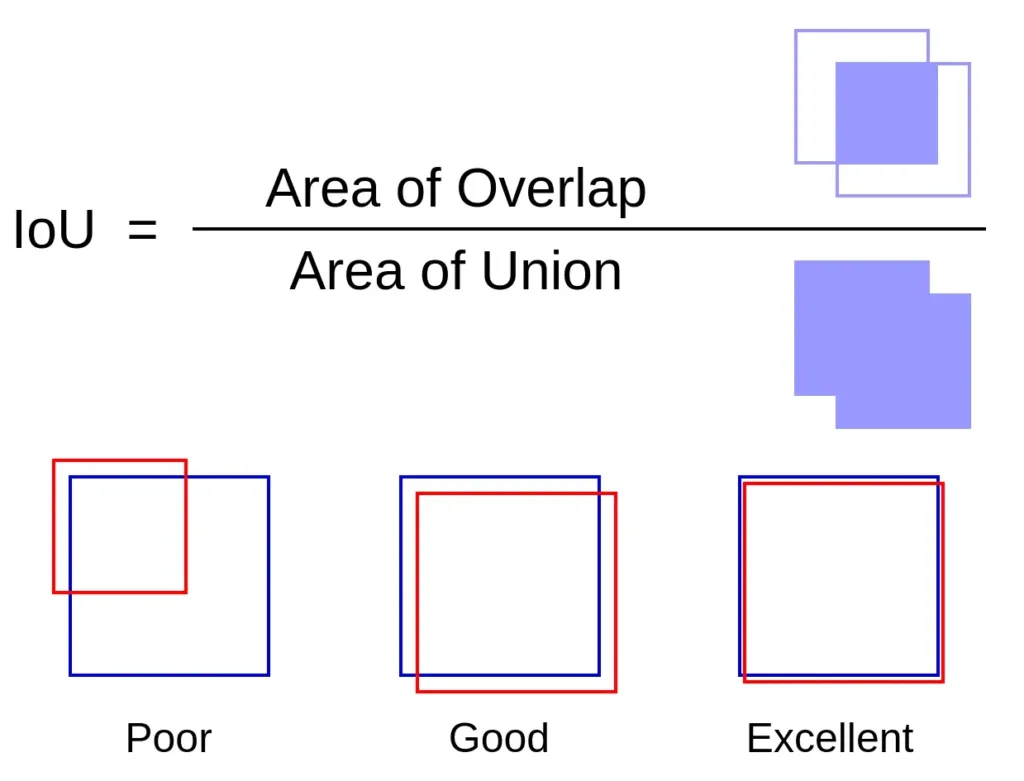
\includegraphics[width=0.5\linewidth]{img/iou.png}
    %\vspace{0.5cm}
    \caption{A diagram representing the Intersection over Union (IoU)}
    \label{metric:iou}
\end{figure}

This metric is crucial in assessing the performance of semantic segmentation models as it provides a quantitative measure of how well the model is able to localize objects within an image. A higher IoU score signifies better localization accuracy and thus, better performance of the detection algorithm.

Furthermore, IoU is often used as a threshold for determining true positives, false positives, and false negatives in object detection tasks, thereby enabling the calculation of other performance metrics such as precision, recall, and F1-score.

% \subsection{Average Precision}
% In the context of image segmentation, Average Precision (AP) remains a crucial performance metric, providing insight into the accuracy of algorithms in segment the object boundaries. Unlike object detection, where bounding boxes are evaluated, segmentation assesses pixel-wise classification, making AP a valuable tool for quantifying segmentation quality on the predicted object mask.

% To compute AP in segmentation, precision and recall are calculated differently compared to object detection. Here, precision measures the ratio of correctly classified pixels (true positives) to the total number of pixels classified as positive (true positives and false positives). Recall, on the other hand, assesses the ratio of correctly classified pixels to the total number of ground truth positive pixels (true positives and false negatives).

% The calculation of AP involves generating a precision-recall curve by varying the segmentation threshold, which determines what constitutes a positive prediction. At each threshold, precision and recall values are computed, and the area under this curve (AUC) represents the AP score. Higher AP values indicate better segmentation performance, capturing both the precision and recall of the segmentation algorithm across different thresholds.

% AP in segmentation is particularly useful for evaluating the ability of algorithms to accurately delineate object boundaries and handle class imbalance within images. It provides a comprehensive assessment of segmentation quality, considering both the accuracy of positive predictions and the ability to capture all relevant objects in the scene.

% When used alongside other segmentation metrics such as Intersection over Union (IOU) or Dice coefficient, AP contributes to a more nuanced understanding of segmentation algorithm performance, helping researchers and practitioners choose the most suitable models for their specific applications.

\section{Watermark Removal}
In this section, we will run experiments on our pipeline. As mentioned in Section \ref{sec:pipeline}, our watermark removal pipeline consists of two main stages: watermark localization and image inpainting. For an image containing a watermark, we first try to identify the location of the watermark, then cover it up and proceed with inpainting using a diffusion model. In the following subsections, we will detail the models and specific methods for each stage, carry out the watermark removal process in these two stages on the dataset mentioned in Section \ref{sec:dataset}. The experimental results and evaluations will also be provided, showing the overall performance of the pipeline on the task of attacking on the watermark.

\label{sec:removal}
\subsection{Watermark Localization}
\subsubsection{Localization methods}
Locating the region to determine where we should attack is a crucial aspect of our proposed pipeline, as we believe it will help improve the results of watermark removal. At this stage, with the watermarked image and its ground truth of the watermark object on the original image as mentioned in Section \ref{sec:embedding}, we will explore methods to localize the watermark's position in the image. This includes identifying information such as the object's boundary, the minimal bounding box of the region containing the watermark, or even using a mask to indicate the watermark's precise location.

\begin{figure}[t]
    \centering
    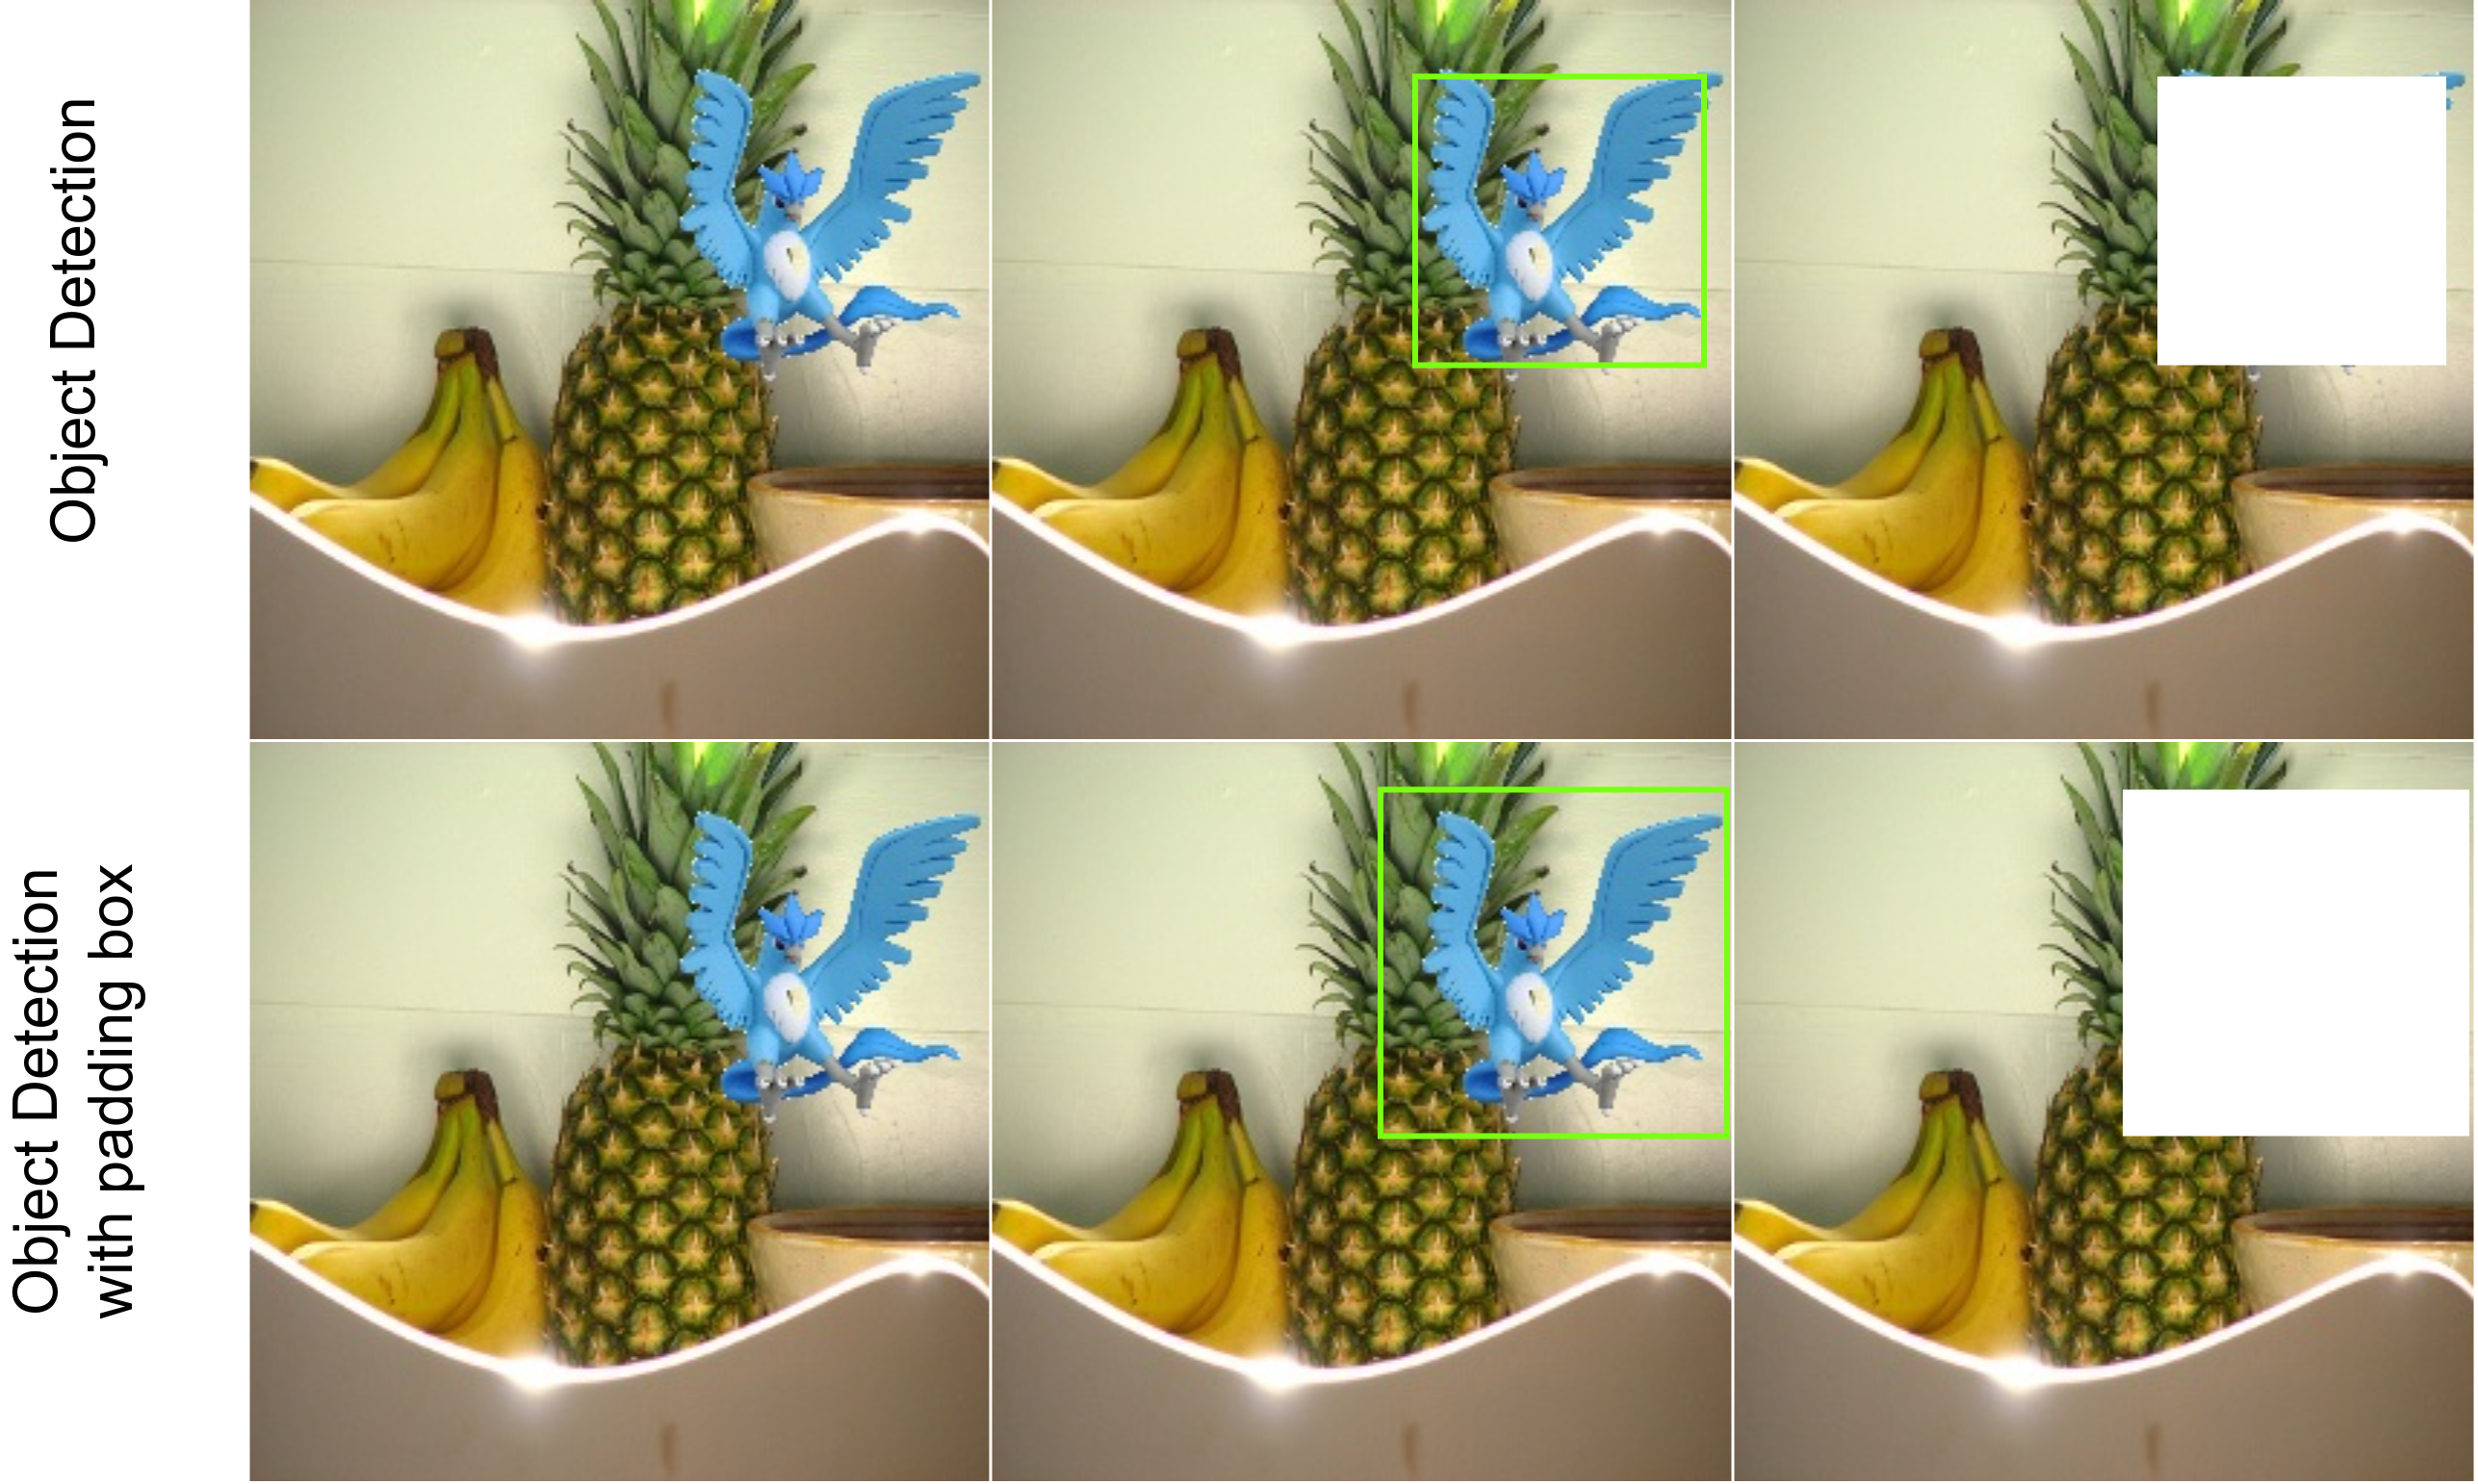
\includegraphics[width=0.8\linewidth]{img/od_w_postprocess.png}
    %\vspace{0.5cm}
    \caption{Localize the watermark with object detection and its post-processing}
    \label{fig:od_w_postprocess}
\end{figure}

There are many ways to localize a watermark in an image. In computer vision and deep learning, we can identify it using models of object detection or segmentation. The object detection method may yield a better result since it only needs to identify the bounding box where the object is, instead of segmentation, which requires per-pixel classification to detect the exact region of the object with a mask. Therefore, applying the object detection method can provide better accuracy and simple post-processing step by adding padding to ensure it covers the entire object as show in Figure \ref{fig:od_w_postprocess}. However, in this pipeline, we decided to use the segmentation method to identify the watermark instead of object detection. The reason for this decision will be illustrated in Figure  \ref{fig:localize-compare-OD-segment}.

\begin{figure}[t]
    \centering
    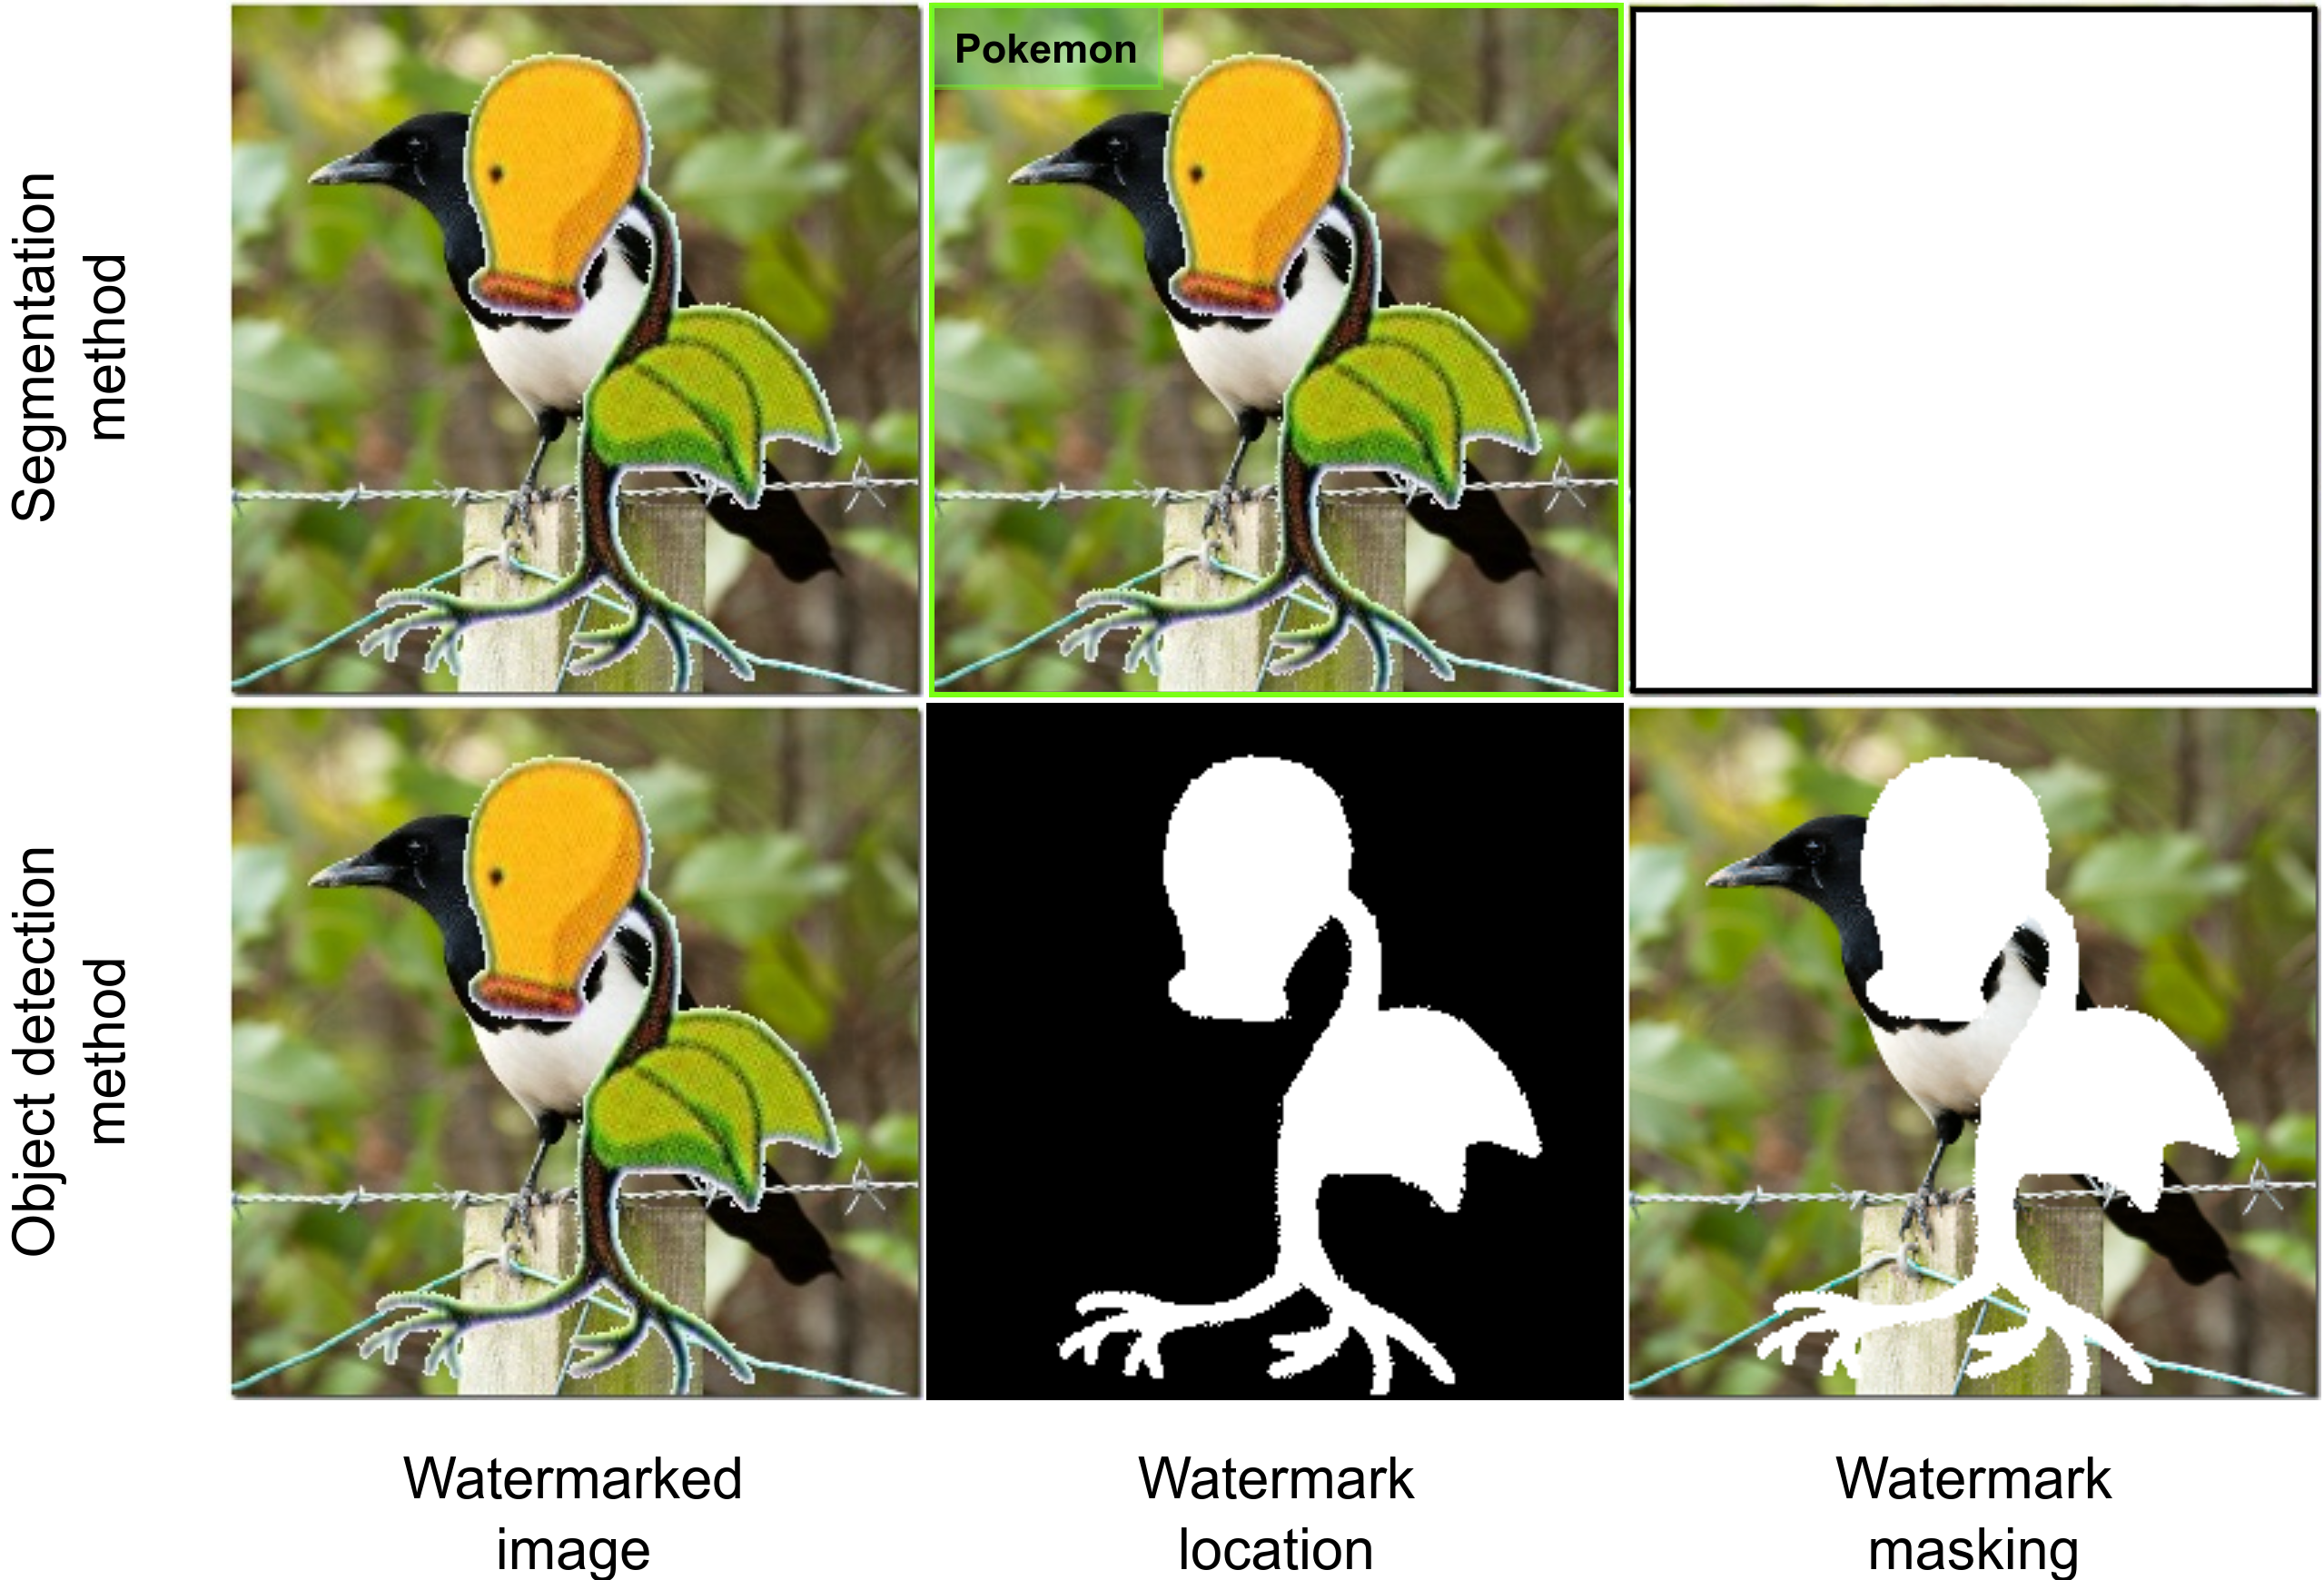
\includegraphics[width=0.8\linewidth]{img/od-segmentation-compare.png}
    %\vspace{0.5cm}
    \caption{Localize the watermark object with object detection and segmentation method}
    \label{fig:localize-compare-OD-segment}
\end{figure}

In Figure \ref{fig:localize-compare-OD-segment}, we can see that the watermark object occupies a large portion of the image. At this point, we can use object detection and semantic segmentation to identify the location of the watermark. In the second column of Figure \ref{fig:localize-compare-OD-segment}, we observe that when using the object detection method, the bounding box of the object occupies almost 100\% of the image area, whereas in reality, the watermark object occupies just over 60\% of the image area. Furthermore, in the next step, after identifying the watermark, we will cover the watermark area and restore the image using image inpainting. With nearly the entire image being covered in this way, performing the next step is completely impractical because there is no information left to be restored, as shown in the last column of Figure \ref{fig:localize-compare-OD-segment}. On the other hand, when using segmentation to identify the location, the watermark object is now identified by a mask that fits the object and occupies exactly the area that the watermark object takes up in the image. This way, we can mask it and reconstruct the image while ensuring that information in the image unrelated to the watermark object is not lost. Hence, we decided to use the segmentation method to localize the watermark object in our pipeline.

\subsubsection{Semantic Segmentation with SegFormer Model}

As mentioned in Section \ref{intro:segformer}, SegFormer \cite{xie2021segformer} is a segmentation model with a transformer-based architecture. The transformer architecture enhances the accuracy of models in computer vision in general and segmentation in particular. Unlike the first segmentation model using transformers, SERT \cite{zheng2021rethinking}, our team chose a lighter model due to resource limitations, but still ensures accuracy in segmentation, which is SegFormer. The performance of the SegFormer and its efficiency will be illustrated in Figure \ref{fig:SegFormer-chart-performance}.

\begin{figure}[t]
    \centering
    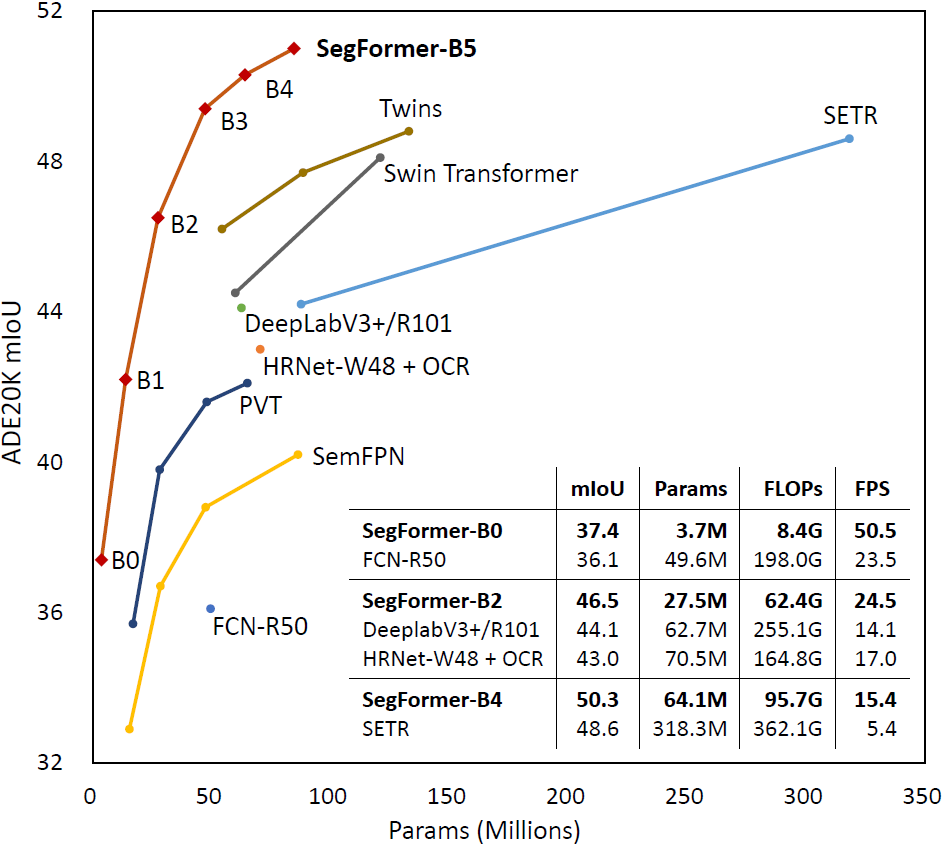
\includegraphics[width=0.5\linewidth]{img/segformer-performance.png}
    %\vspace{0.5cm}
    \caption[SegFormer and other model performance]{SegFormer performance vs. model efficiency on ADE20K dataset compare to other segmentation models \cite{xie2021segformer}}
    \label{fig:SegFormer-chart-performance}
\end{figure}

To train the SegFormer model for watermark localization, we prepared a dataset consisting of approximately 39,000 images containing 50 types of watermarks, with segmentation mask labels of the watermark objects as detailed in Section \ref{sec:embedding}. The model was trained for about 9 hours on an NVIDIA RTX A4500 GPU. After training, we obtained the segmentation results on the validation dataset, which are described in the second row of Figure \ref{fig:segmentation-result}.

\begin{figure}[t]
    \centering
    \includegraphics[width=\linewidth]{img/segmentation-result.png}
    %\vspace{0.5cm}
    \caption[Segmentation result]{Segmentation result when training with SegFormer and Zero-shot inference by prompts with SAM}
    \label{fig:segmentation-result}
\end{figure}

From the results in the second row of Figure \ref{fig:segmentation-result}, we observe that SegFormer yields notable results in segmenting the watermark in the image. The results in the figure show that when we tested the segmentation inference with SegFormer on the validation dataset, the watermark object, which is the Pokémon, was segmented very well from the image. Compared to other methods shown in the figure, SegFormer outperformed them in this validation test by maintaining the consistency of the watermark across various environments of the original image and achieving accurate segmentation from the image. We also evaluated the results using the mIOU metric, which indicates that we achieved 93.22\% on our dataset, demonstrating excellent performance in localizing the watermark in the image.


\subsubsection{Zero-shot Segmentation with Segment Anything Model (SAM)}
The results achieved for localizing watermark objects in images using the SegFormer model are very promising. However, we are interested in exploring a new method. By using an off-the-shelf image inpainting model, we have an idea to investigate a method that can identify watermarks without the need for training. This means that we can run our watermark attacking pipeline without the need to train on a new dataset, also known as a zero-shot pipeline.

After research, we discovered a recent state-of-the-art (SOTA) model that allows us to do just that, called the Segment Anything Model (SAM) developed by Facebook. As mentioned in Section \ref{sec:intro-sam}, the SAM model allows us to segment any object in an image using points or box prompts. Now, we will conduct experiments on this model by preparing prompts using points or boxes and then running the model along with evaluations.

We start with experimenting using a 1-point prompt. We also experimented on our validation dataset with 7500 images and 50 types of watermarks. The 50 types of watermarks are fixed, so we prepare point prompts by identifying a point to select on each watermark object so that the watermark object area when inferred through the SAM model is as complete as possible. Then, combining with the location information of the watermark object in the images we saved, we will determine the points to select for the images so that the model can best segment the watermark area. From what we have prepared, we will inference through SAM and obtain the results in the third row of Figure \ref{fig:segmentation-result}.

From the results  shown in the third row of Figure \ref{fig:segmentation-result}, we can see that by using a 1-point prompt, we can identify the watermark object mask in some cases, such as the first image or the fourth image in the row. However, using a 1-point prompt when inferring with SAM sometimes causes the model to not fully understand what object it needs to identify. For example, in the third or the last image in that row, we can see that SAM considers a large area of surrounding objects as part of the object selected with the 1-point prompt. This can happen due to similarities in color or edges of the objects being adjacent to each other. Moreover, when calculating the accuracy using the mIOU metric for the experiment with the 1-point prompt for SAM, we obtained a result of 75.72\% for using the 1-point prompt to identify the watermark object. While this is not an very impressive score, it demonstrates that this method is feasible for zero-shot segmentation for our watermark dataset. This is because SAM provides better input prompts that we can continue to experiment with and evaluate.

With the results obtained from the 1-point prompt, we realize the potential of SAM in serving as a zero-shot model for our problem. Furthermore, the SAM model allows us to input more than one point for the prompt. Therefore, we continue experimenting by selecting the four best points for each watermark object. Similarly to the 1-point prompt, we have prepared 4-point prompts and inference through SAM on the validation dataset. The results of this experiment are described in the forth row of Figure \ref{fig:segmentation-result}.


From the results shown in the forth row of Figure \ref{fig:segmentation-result}, we can see that now, the objects are segmented much better compared to using only a single point. This is because SAM can be provided with more information related to the object we need to identify in the image, allowing the model to make predictions that closely match the object of interest. By using a 4-point prompt, from the inference test images we obtained, we can see that the watermark object is fully segmented and the likelihood of including surrounding objects is minimized. Moreover, in the fifth image in the row, we can see that the Pokémon shaped like a tree is segmented by SAM even better than by SegFormer, despite the trunk's color being similar to the background, which could potentially cause confusion in the model. Based on the very promising results observed in the inference images, we proceeded to evaluate SAM with a 4-point input prompt on the same validation dataset. The results were extremely impressive, with the mIOU score of SAM with a 4-point prompt being 91.56\%, a very high accuracy rate, especially considering that the model had never seen any training data before.

Using the 4-point prompt yields extremely good results, and we are truly impressed with a zero-shot model, a model that can segment even without being trained on our dataset. Additionally, SAM also supports inputting bounding boxes as prompt, and from there, the model will predict the object to segment in that box region. Therefore, we will utilize the bounding box information prepared in Section \ref{sec:embedding} to use it as input prompt for SAM. By using this method, we obtain the results shown in the last row of Figure \ref{fig:segmentation-result}.

From the results shown in the last row of Figure \ref{fig:segmentation-result}, we can see that by using a bounding box, we can limit the model's observation area and help SAM segment the desired object more easily than by examining the entire image. The results show that using a box prompt also yields better results compared to using a 1-point prompt. Moreover, when watermark objects are confined by a bounding box, the model seems to better understand the differences between the watermark object and other objects in the image, allowing SAM to segment the watermark more clearly than when using a 1-point prompt, which results in a segmentation mask that covers both the watermark and other objects. The evaluation results of the box prompt when running experiments on the validation set showed an mIOU metric of 86.61\%. Although this result is not as good as the 4-point prompt, it opens up a new direction where we can combine object detection and segmentation models to create a higher accuracy zero-shot model in the future.

Finally, we have compiled all the results and evaluations of the segmentation models after experimenting and evaluating on our validation dataset of 7500 images in Table \ref{table:segmentation-result}. From this result table, we can see that using SegFormer for the task of watermark localization in images yields the best result with an mIOU evaluation of 93.22\%. Following that, using SAM with 4-points prompt produces unexpected results of 91.56\%, which is quite good compared to SegFormer even though this is a zero-shot model that has never seen any data before. With the results from this table, we can conclude that using SegFormer is suitable for known watermarks, where we have data to train on and it yields the best results. On the other hand, for unseen watermarks, using SAM is entirely reasonable as it produces very good results, only lagging behind SegFormer by about 2.3\% in mIOU evaluation but without the need for retraining.

\begin{table}[t]
\centering
\begin{tabular}{ll}
\hline
\multicolumn{1}{c}{\textbf{Method}} & \multicolumn{1}{c}{\textbf{mIOU↑}} \\ \hline
\textbf{SegFormer}                             & \textbf{93.22}                                                        \\
SAM with one point                    & 75.72                                                        \\
SAM with four point                   & 91.56                                                        \\
SAM with bounding box                 & 86.61                                                        \\ \hline
\end{tabular}
\caption{Semantic Segmentation evaluation of different methods}
\label{table:segmentation-result}
\end{table}

% \textcolor{red}{Identification -> Localization, change in chart pipeline}

% \textcolor{blue}{
%     In the previous section (Section \ref{sec:ewi}), we have embedded watermarks into images by using image processing method. Then, we need to develop ways to identify them in the watermarked image. In this section, we alleviate the models of segmentation to address this problem.
%     \\
%     1. What is localization. 
%     \\
%     2. There are many ways to identify the watermark in image. In computer vision and deep learning, we can identify it by using models of object detection and segmentation. However, in this pipeline, we decide to use the segmentation method to identify the watermark instead of object detection. The reason will be illustrated in Figure <a figure>
%     \\
%     <Insert some figure here>
%     \\
%     3. From this figure, we can observe that by using object detection, the watermark will be detected at full of this image...\\
%     4. First, we present our result of segmentation when using a transformer-based model, which call SegFormer, that we have introduce in Section...\\
%     5. By using SegFormer, we have archive a notable result on segmentation the watermark in the image, the result is shown in Table ... \\
%     6. However, by using the off-the-shell image inpainting model, we have an idea to make our pipeline is training-free, which mean that we are able to run our watermark attacking pipeline without training on new data, or we also called a zero-shot pipeline. We are going to make it possible by using the recently SOTA zero-shot model, Segment Anything developed by Facebook. 
% }



\subsection{Image Inpainting}
In this section, we will conduct experiments on the inpainting task using the I$^2$SB model. We will perform experiments for the image inpainting task on both the ImageNet dataset, which is a pretrained dataset for I$^2$SB, and other data that we collected, which differ from the original training dataset. Through these experiments, we obtained several results, which are presented below.

\subsubsection{Image Inpainting with ImageNet}
First, we will conduct experiments using the I$^2$SB model on the ImageNet dataset. We will utilize the ground-truth watermark mask extracted in Section \ref{sec:embedding} to create a corrupted image by applying this mask. Subsequently, we will forward the corrupted image through the I$^2$SB model for reconstruction. The results obtained will be described in Figure \ref{fig:i2sb-imagenet-result}.

From Figure \ref{fig:i2sb-imagenet-result}, we can observe that in the first two columns of results, the reconstructed images are very well-done and closely resemble the original images. Particularly in the second column, where the leaf is partially obscured with intricate patterns, and the corrupted image has almost completely covered the leaf, our model has reconstructed it remarkably well, almost identical to the original image. However, it is reasonable that image inpainting might produce some details different from those in the original image; even when looking at a corrupted image, we can only guess what details might lie beneath that mask without being certain until we see a clean image. This is evident in the third and fourth columns. In these images, the patterns on the body of the leopard and the face of the dog have been reconstructed. If we had not seen the clean image, we could see that the model can understand what it needs to draw and is doing a good job of reconstructing the image with many details obscured in the corrupt image.

Moving to the last two columns of results, we can see that the masks have now covered the face of the dog and the chemical flask. In the reconstructed image of the dog, we can see that details such as the teeth or the nose hole have changed slightly, but the expression of the dog remains cheerful like in the original image. In terms of detail, the model is producing an image with many details changed because they were obscured, but the details it guesses are quite reasonable and fit well with the context of the image. In the last image, a chemical flask with a text label is reconstructed. At this point, the model has restored the shape of the flask quite intact and well, but the text on the flask has been altered and is no longer readable. For an inpainting model, guessing what is under the mask with text is extremely difficult, but the fact that they understand there are characters beneath the mask and can reconstruct them is quite promising and lays the foundation for handling text in the future.

\begin{figure}[t]
    \centering
    \includegraphics[width=0.8\linewidth]{img/i2sb-imagenet-result.png}
    %\vspace{0.5cm}
    \caption[Image Inpaiting using I$^2$SB model with ImageNet dataset]{Image Inpaiting using I$^2$SB model with ImageNet dataset}
    \label{fig:i2sb-imagenet-result}
\end{figure}
It is impressive to see such high scores on both PSNR and SSIM metrics, indicating excellent performance in image reconstruction. PSNR of 30.2 falls within the range considered good (30-40), and an SSIM score of 0.96 indicates extremely high structural similarity between the reconstructed and original images. These results demonstrate the effectiveness of the I$^2$SB model in reconstructing images, even in cases where significant portions of the image are missing or corrupted.
\subsubsection{Image Inpainting with other dataset}
After running experiments for the image inpainting part using I$^2$SB on the pre-trained ImageNet dataset, we will continue to perform experiments by running this model with datasets outside the training data. As mentioned in Section \ref{sec:i2sb}, the I$^2$SB model has the ability to reconstruct images with part of the information not masked instead of starting from Gaussian noise like other diffusion-based models. This enables the model to run completely on data outside our trained data. Indeed, when collecting data outside the training data, we tried running the I$^2$SB model with watermark object masks and obtained the results described in Figure \ref{fig:i2sb-difference-dataset-result}.

\begin{figure}[t]
    \centering
    \includegraphics[width=0.8\linewidth]{img/i2sb-difference-dataset-result.png}
    %\vspace{0.5cm}
    \caption[Image Inpaiting using I$^2$SB model with random dataset]{Image Inpaiting using I$^2$SB model other dataset}
    \label{fig:i2sb-difference-dataset-result}
\end{figure}

From the results shown in Figure \ref{fig:i2sb-difference-dataset-result}, we can see that the results obtained from the images outside the training dataset are indeed promising. Despite differences in detail, the model successfully reconstructs parts of the images that were covered or missing, even though they were not present in the training set. This demonstrates the generalization capability of the I$^2$SB model, allowing it to be applied to various datasets without the need for retraining. Furthermore, there is potential for further improvement through additional processing techniques or model tuning to enhance results on more diverse datasets without the need for retraining.

\subsection{Watermark Removal Pipeline}
In this section, after building the watermark localization model and the image inpainting model with a mask, we will complete our two-stage pipeline for watermark removal. At the same time, we will observe, evaluate, and compare the results of watermark removal on our pipeline with other methods.
\subsubsection{CNN-based method}

Recently, while researching models related to the watermark removal problem, we came across a paper called SWCNN \cite{2024swcnn}. This paper was published in 2024 and submitted to the CVPR conference. The paper designs a CNN-based model for the watermark removal task, and it claims to achieve state-of-the-art (SOTA) results compared to previous papers, even outperforming a method using generative models like GAN. The reported results are based on the evaluation table provided by the paper, presented in Table \ref{table:swcnn}.

\begin{table}[t]
    \centering
    \begin{tabular}{cccll}
        \hline
        \textbf{Methods}                             & \textbf{PSNR ↑}  & \textbf{SSIM ↑} \\ \hline
        FFDNet  \cite{zhang2018ffdnet}               & 27.8820          & 0.8778          \\
        DIP  \cite{ulyanov2018deep}                  & 29.7473          & 0.9260          \\
        WGAN-GP  \cite{yu2018generative}             & 31.0752          & 0.9662          \\
        DnCNN  \cite{zhang2017beyond}                & 30.1071          & 0.9620          \\
        {DRD-Net \cite{deng2019drd}}                 & 28.9090          & 0.9707          \\
        {FastDerainNet \cite{wang2020fastderainnet}} & 32.2593          & 0.9815          \\
        {EAFNWDD \cite{sun2021efficient}}            & 33.4744          & 0.9700          \\
        \textbf{SWCNN} \cite{2024swcnn}              & \textbf{36.9022} & \textbf{0.9893} \\ \hline
    \end{tabular}
    \caption[Watermark removal performance of different methods]{Watermark removal performance of different methods\cite{2024swcnn}}
    \label{table:swcnn}
\end{table}

From there, we set up to train this model on our dataset. We prepared the same training and validation dataset, along with the 50 types of watermarks used for evaluating our pipeline. After training for 5 hours, we obtained the results of this model. The performance of the model when trained and tested on our dataset is approximately 25.64 on the PSNR metric and 0.85 on the SSIM metric. The results are summarized in Table \ref{table:swcnn}.

\subsubsection{Our Pipeline with Segmentation and Image Inpainting}

After preparing the necessary models, we finally combined them and started running our pipeline. Firstly, for Watermark Localization, we performed inference and observed that although the SegFormer model had been trained and produced very good results, there were still some errors in the segmentation mask results, as shown in Figure \ref{fig:segformer-no-dilate}.

\begin{figure}[t]
    \centering
    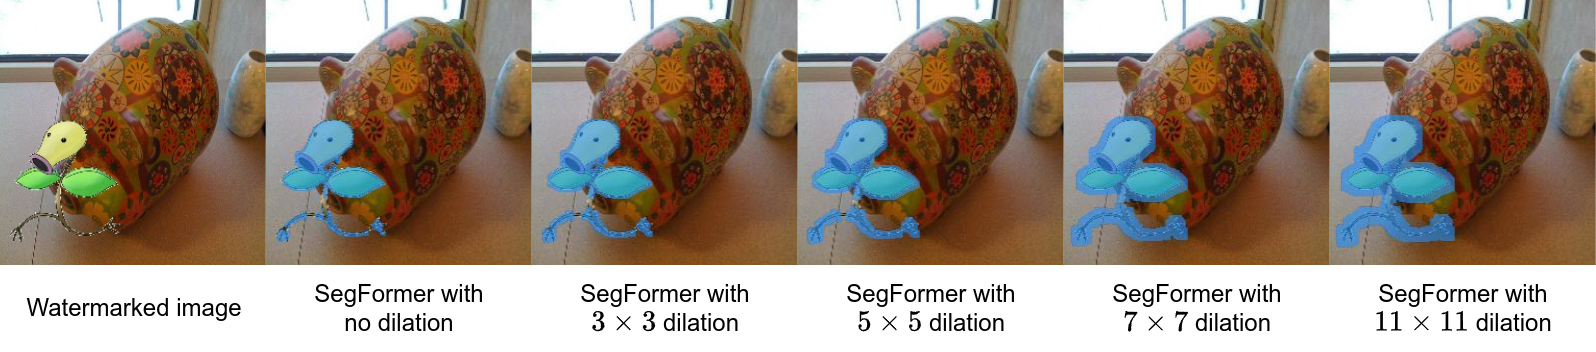
\includegraphics[width=\linewidth]{img/dilation-segformer.png}
    %\vspace{0.5cm}
    \caption[SegFormer Segmentation post-processing]{SegFormer Segmentation result with inaccurate mask and post-processing by different dilation kernel}
    \label{fig:segformer-no-dilate}
\end{figure}

From Figure \ref{fig:segformer-no-dilate}, we can see that the resulting segmentation mask may still have some shortcomings, especially in cases where the watermark object has a color similar to objects in the image. To address this, we experimented with a post-processing method called dilation. Dilation is a technique that extends the segmentation mask, allowing erroneous parts of the mask to be connected, thus helping to fully encompass the object in a single mask. However, when applying the dilation method, we need to select the kernel size carefully, as different kernel sizes will yield different results. We conducted experiments to select an appropriate kernel size, and the results are shown in Table \ref{fig:segformer-no-dilate} and Figure \ref{fig:segformer-no-dilate}.

From the experimental results on various dilation kernels, we can see that if we use small kernels like $3 \times 3$ or $5 \times 5$, the continuity of the segmentation mask is still not fully improved. With the use of a $7 \times 7$ kernel, our segmentation mask has been completely connected and can greatly improve the results. With larger kernel sizes, as we can observe in Table \ref{fig:segformer-no-dilate} and Figure \ref{fig:segformer-no-dilate}, using a larger kernel than necessary will inflate our segmentation mask, causing the image inpainting model to predict on a larger mask, thereby reducing the model's evaluation metrics.

\begin{table}[t]
    \centering
    \begin{tabular}{lll}
        \hline
        \multicolumn{1}{c}{\textbf{Method}}                                                & \multicolumn{1}{c}{\textbf{PSNR ↑}} & \multicolumn{1}{c}{\textbf{SSIM ↑}} \\ \hline
        SegFormer + I$^2$SB & 25.13                                & 0.87                                 \\ 
        SegFormer + I$^2$SB + ($3 \times 3$) dilation & {25.81}                       & {0.88}                        \\ 
        SegFormer + I$^2$SB + ($5 \times 5$) dilation & {25.82}                       & {0.88}                        \\ 
        SegFormer + I$^2$SB + ${(7 \times 7)}$ {dilation} & \textbf{27.82}                       & \textbf{0.90}                        \\ 
        SegFormer + I$^2$SB + ($11 \times 11$) dilation & {26.82}                       & {0.89}                        \\ \hline
    \end{tabular}
    \caption{Segmentation post-processing performance with different settings}
    \label{table:segformer-kernel}
\end{table}
With the experimentation of dilation post-processing for the segmentation mask as previously conducted, we will now proceed with the watermark removal pipeline by applying dilation with a kernel size of $7 \times 7$ to ensure the accuracy of the segmentation mask. The results obtained from our pipeline are summarized in Table \ref{table:wtm-rmv}. From this table, we can observe that the combination of SegFormer and I$^2$SB for our pipeline is yielding the best results in terms of PSNR evaluation with a score of 27.82 along with a metric score of 0.90 for SSIM. This result is highly impressive as it closely approaches the results of using I$^2$SB on the ImageNet dataset. Moreover, this result outperforms the results of SWCNN, a paper that claims to produce the best results for watermark removal and has beaten several GAN models for this task. Furthermore, another notable result is the combination of SAM with a 4-point prompt and I$^2$SB also yields extremely high results, even the best on the SSIM metric with a score of 0.91. This is noteworthy as the combination of SAM and I$^2$SB is an idea for a Zero-shot pipeline, where we can use a watermark removal pipeline without the need to retrain on new data.
\begin{table}[!t]
    \centering
    \begin{tabular}{lll}
        \hline
        \multicolumn{1}{c}{\textbf{Method}}                                                & \multicolumn{1}{c}{\textbf{PSNR ↑}} & \multicolumn{1}{c}{\textbf{SSIM ↑}} \\ \hline
        Labeled mask + I$^2$SB    & \textbf{30.2}                        & \textbf{0.96}                        \\ \hline
        SWCNN  \cite{2024swcnn}                                                                             & 25.64                                & 0.85                                 \\  \hline
        SegFormer + I$^2$SB & 25.13                                & 0.87                                 \\ 
        SegFormer + I$^2$SB + dilation & \textbf{27.82}                       & {0.90}                        \\ \hline
        SAM with 1 point + I$^2$SB + dilation  & {21.71}                       & {0.80}                        \\
        SAM with 4 points + I$^2$SB + dilation  & {25.92}                       & \textbf{0.91}                        \\ 
        SAM with boxes + I$^2$SB + dilation & {24.76}                       & {0.89}                        \\ \hline
    \end{tabular}
    \caption{Watermark removal performance of different methods}
    \label{table:wtm-rmv}
\end{table}

% \textcolor{red}{- Bỏ center mask đi, dùng phần random mask rồi viết lại phần kết quả của chạy riêng I2SB cho labeled mask
% \\
% - Nhắc lại phần identify watermark -> kết quả của segformer w/o dilation
% \\
% - Nói về việc Dialate mask (dùng kernel 7x7 qua 1 vòng dilate) để mở rộng phần xác định wtm -> ra kết quả tốt hơn
% \\
% - Giải thích thêm về chọn kernel dialate và list kết quả trên các kernel khác (3x3, 5x5, 9x9, 11x11)
% \\
% - Thử xem lại loss segmentation để lập luận cách xác định kích thước kernel dilation
% \\
% - Các kết quả của data mình trong các related work
% \\
% - SCOPE: Tập trung xử lý ảnh -> xử lý visible watermark}


% \section{Write for DEMO}
\chapter{Conclusion}
\thispagestyle{empty}
\section{Summary}

This capstone project offers a valuable opportunity to delve into essential areas of mathematics, showcasing the elegance of logical reasoning in this field and its applicability to machine learning. Our study builds progressively across several branches, including real analysis, measure theory, probability and stochastic processes, and ultimately, stochastic differential equations (SDEs). We have compiled the necessary theorems for the reverse-time equation, the foundational element for diffusion models using SDEs. Additionally, we have thoroughly explored the Transformer neural network architecture, focusing on its Positional Embedding and Attention Mechanisms.

On the practical side, we conducted experiments with various segmentation and inpainting models to identify the most effective methods for watermark removal. Throughout this process, we addressed and resolved technical challenges related to performance and memory, enhancing our engineering skills in the field of Artificial Intelligence. The result is a comprehensive pipeline that processes a watermarked image and outputs an unwatermarked version while preserving the original structure of the image. Additionally, our pipeline outperforms some methods when using the two-stage pipeline, which involves localizing the watermark first and then removing it, making it possible to improve sub-task models. Furthermore, we experimented with and achieved noticeable results on a Zero-shot pipeline, making our model flexible to use on any dataset.



\section{Limitations and Future Work}
\subsection{Limitation}
% \subsubsection{Processing Time}

% \subsubsection{Processing Time}

In our pipeline, it takes about 1.5-2.5 seconds to complete one inference, which is quite time-consuming and may require users to wait if they want to remove watermarks from multiple images. Additionally, our problem is limited to visible watermarks and focuses on processing images, without deep exploration and development on other types of watermarks. Furthermore, our watermark dataset is small, as it only covers Pokemon-themed watermarks and lacks generalization to all visible watermarks. For the zero-shot methods we implemented in this report, they still require detailed instructions from users, such as points or boxes, and have not been tested on more natural instructions like language or simply a text sentence. We will continue to research and improve our limitations in the future. 


\subsection{Future Work}
In the future work, we will develop Zero-shot methods using text prompts. We find this to be entirely feasible as we experimented with a model that allows us to align images and text, namely CLIP \cite{radford2021learning}. This model is trained on hundreds of thousands of image-text pairs with the aim of learning mutual features and can be used as a feature extraction layer, where the text prompt provides the class that the image is associated with, allowing the model to generate attention heatmaps on the image, highlighting objects related to the prompted text. The results of our experiments with the pretrained CLIP model on watermark data are shown in Figures \ref{fig:pic_of_pokemon} and \ref{fig:pic_of_wtm}.

In Figures \ref{fig:pic_of_pokemon} and \ref{fig:pic_of_wtm}, we can see that when prompted with "Pokemon," the model immediately focuses on the Pokémon in the center of the image, and when prompted with "Watermark," the model provides some points that are likely watermarks. By using CLIP in this way, we can leverage it to extract features from text prompts and make accurate predictions as needed.
\begin{figure}[t]
    \centering
    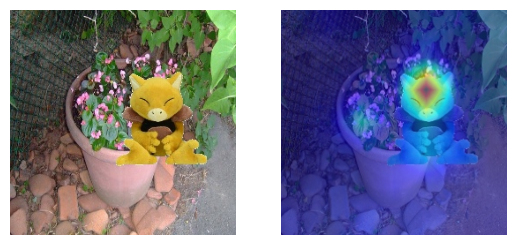
\includegraphics[width=0.75\linewidth]{img/pic_of_pokemon.png}
    \caption{CLIP attention heatmap with text prompt \textit{The picture have pokemon}}
    \label{fig:pic_of_pokemon}
\end{figure}

\begin{figure}[t]
    \centering
    \includegraphics[width=0.75\linewidth]{img/pic_of_wtm.png}
    \caption{CLIP attention heatmap with text prompt \textit{The picture have watermark}}
    \label{fig:pic_of_wtm}
\end{figure}

\begin{figure}[t]
    \centering
    \includegraphics[width=0.75\linewidth]{img/groundedsam.png}
    \caption[Zero-shot text prompt result with Object Detection and SAM box prompt]{Zero-shot text prompt \textit{The picture have pokemon} result with Object Detection and SAM box prompt}
    \label{fig:groundedsam}
\end{figure}
Furthermore, in our experiments with SAM, we found that using bounding boxes as input for SAM is entirely promising. We have researched and are developing a model related to Zero-shot object detection using text prompts. The trial results of our team are shown in Figure \ref{fig:groundedsam}. Specifically, in this image, we also used the prompt "\textit{The picture has pokemon}" to indicate that there are Pokémon in this image, even though the model has never learned about Pokémon before. Nonetheless, it still makes predictions of two potential bounding boxes. From there, the team used these bounding boxes as input for SAM and found that it was able to detect and segment them. However, due to the limited time of the thesis and the results not meeting expectations, the team decided to continue researching this aspect for the next phase.
\chapter*{Appendix}
\addcontentsline{toc}{chapter}{Appendix}
\renewcommand\thetheorem{A.\arabic{theorem}}


\begin{lemma}[Expectation of Powers of a zero-mean Gaussian random variable]
  If $X\sim\N(0,\sigma^2)$, then $\EE[X^2] = \sigma^2$ and $\EE[X^4] = 3\sigma^4$.
\end{lemma}


% \begin{theorem}[Properties of Indicator Functions]
%   \label{theorem:indiprop}
%   Let $(X,\Sigma,\mu)$ be a measure space and $A,B$ be subsets of $\Omega$, then
%   \begin{enumerate}
%     \item $\mathbf{1}_{A\cap B}=\mathbf{1}_A\mathbf{1}_B$.
%     \item $\int\limits_{X}\mathbf{1}_A\d \mu = \mu(A)$.
%   \end{enumerate}
% \end{theorem}

\begin{theorem}[Pointwise Limit of Measurable Functions is Measurable]
  \label{theorem:pointwise-limit-of-measurable-functions-is-measurable}
  Let $(f_n)$ be a sequence of measurable functions converging pointwisely to $f$. Then $f$ is measurable.
\end{theorem}

% \begin{theorem}[Approximation of a Measurable Function]
%   \label{theorem:meafuncapp}
%   Let $(X,\Sigma)$ be a measurable space and $f:\Omega\to\RR$ be a measurable function. Then there exists a sequence of step functions $(f_n)_{n\in\NN}$ that pointwise converges to $f$ i.e.
%   $$\forall x\in X, f(x)=\lim\limits_{n\to\infty}f_n(x).$$
%   If $f\ge0$, we can choose $\{f_n\}$ to be increasing.
% \end{theorem}

\begin{theorem}[Fubini's Theorem]
  \label{theorem:fubini}
  Let $(\Omega,\F,\mu)$ and $(\Gamma,\G,\nu)$ be measure spaces, and $(\Omega\times\Gamma,\F\otimes\G,\mu\times\nu)$ be the product measure space. Then for any measurable function $f:\Omega\times\Gamma\to\RR$,
  \begin{equation}  \int\limits_{\Omega\times\Gamma}f\d (\mu\times\nu) = \int\limits_{\Omega}\int\limits_{\Gamma}f\d \mu\d \nu = \int\limits_{\Gamma}\int\limits_{\Omega}f\d \nu\d \mu.
  \end{equation}
\end{theorem}

\begin{lemma}[Gronwall Inequality]
  \label{lemma:gronwall-inequality}
  Let $f:[0,T]\to\RR$ be continuous function such that
  $$f(t) \le c_1 + c_2 \int_0^t f(s)\d s.$$
  Then $f (t) \le c_1e^{c_2t}$.
\end{lemma}

% \section{General Proof of Theorem \ref{theorem:independent-expectation}}
% \label{proof:independent-expectation}

% \section{The Construction of the Itô Integral}
% \label{appendix:ito}

% \section{The Construction of the Wiener Process}
% \label{brown}
% Consider the set of all real-valued, square-integrable functions defined on $(0, 1)$ i.e. the set of $f(t)$ such that

% $$\int\limits_0^1 f^2(t)\d t<\infty.$$

% We can check effortlessly that this set is a vector space. Let us denote it by $L^2(0,1)$ and define the dot product

% $$\langle f,g\rangle = \int\limits_0^1 f(t)g(t)\d t.$$

% Now we wish to find an orthonormal basis for $L^2(0,1)$. Note that it is an infinite dimensional space. Let $\{\psi_n\}_{n=0}^\infty$ be an orthonormal basis. We must have that

% $$\int\limits_0^1 \psi_i(t)\psi_j(t)\d t = \begin{cases}
%     0,\,\,i\ne j\\
%     1,\,\,i = j
% \end{cases}.$$

% If there is another function $\varphi$ such that $\varphi$ along with $\{\psi_n\}_{n=0}^\infty$ i.e



% In fact, the functions in the orthogonal basis of $L^2(0,1)$ is the Haar functions define below.

% \begin{definition}
%     The family $\{h_k(.)\}_{k=0}^\infty$ of Haar functions is defined for $0\le t\le 1$ as follows:
%     $$h_0(t) = 1,\,\,\text{ for } 0\le t\le 1,$$
%     $$h_1(t)=\begin{cases}
%         1 &\,\,\text{ for } 0\le t\le \dfrac{1}{2}\\
%         -1 & \,\,\text{ for } \dfrac{1}{2}< t\le 1
%     \end{cases}$$
% If $2^n\le k<2^{n+1},\,n=1,2\ldots,$ we set
% $$h_k(t)=\begin{cases}
%         2^{n/2} &\,\,\text{ for } \dfrac{k-2^n}{2^n}\le t\le \dfrac{k-2^n+1/2}{2^n}\\
%         -2^{n/2} & \,\,\text{ for } \dfrac{k-2^n+1/2}{2^n}< t\le \dfrac{k-2^n+1}{2^n}\\
%         0 & \,\,\text{otherwise} 
%     \end{cases}$$
% \end{definition}

% \begin{align*}

% \end{align*}

% \begin{definition}
%     For $k=0,1,2,\ldots$, 
%     $$s_k(t)=\int\limits_{0}^t h_k(t)\d t$$
%     is the $k$th Schauder function.
% \end{definition}

% \section{Proof of Theorem \ref{theorem:score}}
% We have

% \begin{align} 
%     \dfrac{1}{2}\EE_{p_{\text{data}}}[\|\nabla_\xbf\log p(\xbf,\theta)-\nabla_\xbf\log p_{\text{data}}(\xbf)\|^2_2]
%     &=\EE_{p_{\text{data}}}\left[\dfrac{1}{2}\|\nabla_\xbf\log p_{\text{data}}(\xbf)\|^2_2+\dfrac{1}{2}\|s_\theta(\xbf)\|^2_2 - s_\theta(\xbf)^\top \nabla_\xbf\log p_{\text{data}}(\xbf)\right].  
% \end{align}


% The first term in the brackets is a constant and the second term can be computed. Hence we focus on the third term.

% \begin{align}
% \EE_{p_{\text{data}}}[-s_\theta(\xbf)^\top \nabla_\xbf\log p_{\text{data}}(\xbf)] 
% &= -\int_{\xbf\in\RR^D}s_\theta(\xbf)^\top \nabla_\xbf\log p_{\text{data}}(\xbf)p_{\text{data}}(\xbf)\d \xbf\notag\\
% &= -\int_{\xbf\in\RR^D}s_\theta(\xbf)^\top \dfrac{\nabla_\xbf p_{\text{data}}(\xbf)}{p_{\text{data}}(\xbf)}p_{\text{data}}(\xbf) \d \xbf\notag\\
% &= -\int_{\xbf\in\RR^D}s_\theta(\xbf)^\top \nabla_\xbf 
% p_{\text{data}}(\xbf)  \d \xbf
% \end{align}

% We can simplify this further by using integration by parts. Let 

% \begin{equation}
%     s_\theta(\xbf)^\top = 
%     \begin{pmatrix}
%    \varphi_1 (\xbf,\theta) & \ldots & \varphi_D (\xbf,\theta)
%     \end{pmatrix},
% \end{equation}

% \begin{equation}
%     \nabla_\xp_{\text{data}}(\xbf)  = 
%     \begin{pmatrix}
%    \dfrac{\partial p_{\text{data}}(\xbf)}{\partial x_1}\\ \vdots \\\dfrac{\partial p_{\text{data}}(\xbf)}{\partial x_D}
%     \end{pmatrix}.
% \end{equation}
% The equation becomes
% \begin{align}
% -\int_{\xbf\in\RR^D}s_\theta(\xbf)^\top \nabla_\xbf 
% p_{\text{data}} \d \xbf &= -\int_{\xbf\in\RR^D}\sum\limits_{i=1}^D \varphi_i (\xbf,\theta) \dfrac{\partial p_{\text{data}}(\xbf)}{\partial x_i} \d \xbf\notag\\
% &=\sum\limits_{i=1}^D \left[-\int_{\xbf\in\RR^D} \varphi_i (\xbf,\theta) \dfrac{\partial p_{\text{data}}(\xbf)}{\partial x_i} \d \xbf\right]
% \end{align}
% We have 

% \begin{align}
%     \dfrac{\partial \varphi_1 (\xbf,\theta) p_{\text{data}}(\xbf)}{\partial x_1} = \varphi_1 (\xbf,\theta) \dfrac{\partial p_{\text{data}}(\xbf)}{\partial x_1} +  p_{\text{data}}(\xbf)\dfrac{\partial \varphi_1 (\xbf,\theta)}{\partial x_1}.
% \end{align}

% So integrating by $x_1$ over $\RR$ gives

% \begin{equation}
% \label{equation:10}
%     \lim\limits_{x_1\to\infty} \varphi_1 (\xbf,\theta) p_{\text{data}}(\xbf) - \lim\limits_{x_1\to-\infty} \varphi_1 (\xbf,\theta) p_{\text{data}}(\xbf) = \int\limits_{-\infty}^{\infty} \varphi_1 (\xbf,\theta) \dfrac{\partial p_{\text{data}}(\xbf)}{\partial x_1}\d x_1+ \int\limits_{-\infty}^{\infty} p_{\text{data}}(\xbf)\dfrac{\partial \varphi_1 (\xbf,\theta)}{\partial x_1}\d x_1.
% \end{equation}

% Due to the assumed regularity conditions, we have

% \begin{equation}
%     \lim\limits_{x_1\to\infty} \varphi_1 (\xbf,\theta) p_{\text{data}}(\xbf)=\lim\limits_{x_1\to-\infty} \varphi_1 (\xbf,\theta) p_{\text{data}}(\xbf)=0.
% \end{equation}

% Hence (\ref{equation:10}) implies that 
% \begin{equation}
%     -\int\limits_{-\infty}^{\infty} \varphi_1 (\xbf,\theta) \dfrac{\partial p_{\text{data}}(\xbf)}{\partial x_1}\d x_1=\int\limits_{-\infty}^{\infty} p_{\text{data}}(\xbf)\dfrac{\partial \varphi_1 (\xbf,\theta)}{\partial x_1}\d x_1.
% \end{equation}

% Taking integral over $x_2,\ldots,x_D$ yields

% \begin{equation}
%     -\int_{\xbf\in\RR^D} \varphi_1 (\xbf,\theta) \dfrac{\partial p_{\text{data}}(\xbf)}{\partial x_1}\d \xbf=\int_{\xbf\in\RR^D}  p_{\text{data}}(\xbf)\dfrac{\partial \varphi_1 (\xbf,\theta)}{\partial x_1}\d \xbf.
% \end{equation}

% The calculation is similar for $i=2,\ldots,D$. Therefore, 

% \begin{align}
%     \EE_{p_{\text{data}}}[-s_\theta(\xbf)^\top \nabla_\xbf\log p_{\text{data}}(\xbf)] 
%     &= \int_{\xbf\in\RR^D}  p_{\text{data}}(\xbf)\left[\sum\limits_{i=1}^D \dfrac{\partial \varphi_i (\xbf,\theta)}{\partial x_i}\right]\d \xbf\notag\\
%     &=\EE_{p_{\text{data}}}[\mathrm{tr}(\nabla_\xs_\theta(\xbf))].
% \end{align}

% Thus we can define the loss function based on the approximating function only
% \begin{align}
%     \L(\theta) = \EE_{p_{\text{data}}}\left[\mathrm{tr}(\nabla_\xs_\theta(\xbf))+\dfrac{1}{2}\|s_\theta(\xbf)\|^2_2\right].
% \end{align}

\printindex
\printbibliography
\end{document}